\documentclass[openany, oneside]{book}
\usepackage[fontset=none]{ctex}
\usepackage{graphicx} % Required for inserting images
\usepackage{amsfonts, amsmath, amssymb, amsthm, mathtools}
\usepackage{float}
\usepackage{subfig}
\usepackage{color}
\usepackage{hyperref}
\usepackage[bottom=1in]{geometry}
\usepackage{tikz}
\usetikzlibrary{arrows, positioning}
\usepackage[ruled,linesnumbered,noend]{algorithm2e}
\usepackage[style=authoryear,maxbibnames=20,uniquename=false]{biblatex}
\usepackage{fancyhdr}


\setCJKmainfont[ItalicFont=FandolKai]{FandolSong}
\setCJKsansfont{FandolHei}
\setCJKmonofont{FandolKai}

\pagestyle{myheadings}
\markright{\thepage}

\newtheorem{remark}{备注}[section]
\newtheorem{theorem}{定理}[section]
\newtheorem{claim}{断言}[section]
\newtheorem{lemma}{引理}[section]
\newtheorem{corollary}{推论}[section]

\newtheorem*{remark*}{备注}
\newtheorem*{theorem*}{定理}
\newtheorem*{claim*}{断言}
\newtheorem*{lemma*}{引理}
\newtheorem*{corollary*}{推论}

\hypersetup{hidelinks}


\title{CS229 课程讲义}
\author{Andrew Ng (吴恩达) and Tengyu Ma (马腾宇)}
\date{由 Namoe 翻译\\June 2025}

\addbibresource{ref.bib}

\begin{document}

\maketitle

\tableofcontents

\part{监督学习}

不妨先从监督学习的几个例子谈起。假设有一个记录了俄勒冈州波特兰市 47 套房屋的居住面积和价格的数据集:

\begin{table}[h]
    \centering
    \begin{tabular}{c|c}
        居住面积 (平方英尺) & 价格 (1000\$) \\
        \hline
        2104 & 400 \\
        1600 & 330 \\
        2400 & 369 \\
        1416 & 232 \\
        3000 & 540 \\
        $\vdots$ & $\vdots$
    \end{tabular}
    \label{tab:house_example}
\end{table}

将这些数据绘制出来:

\begin{figure}[H]
    \centering
    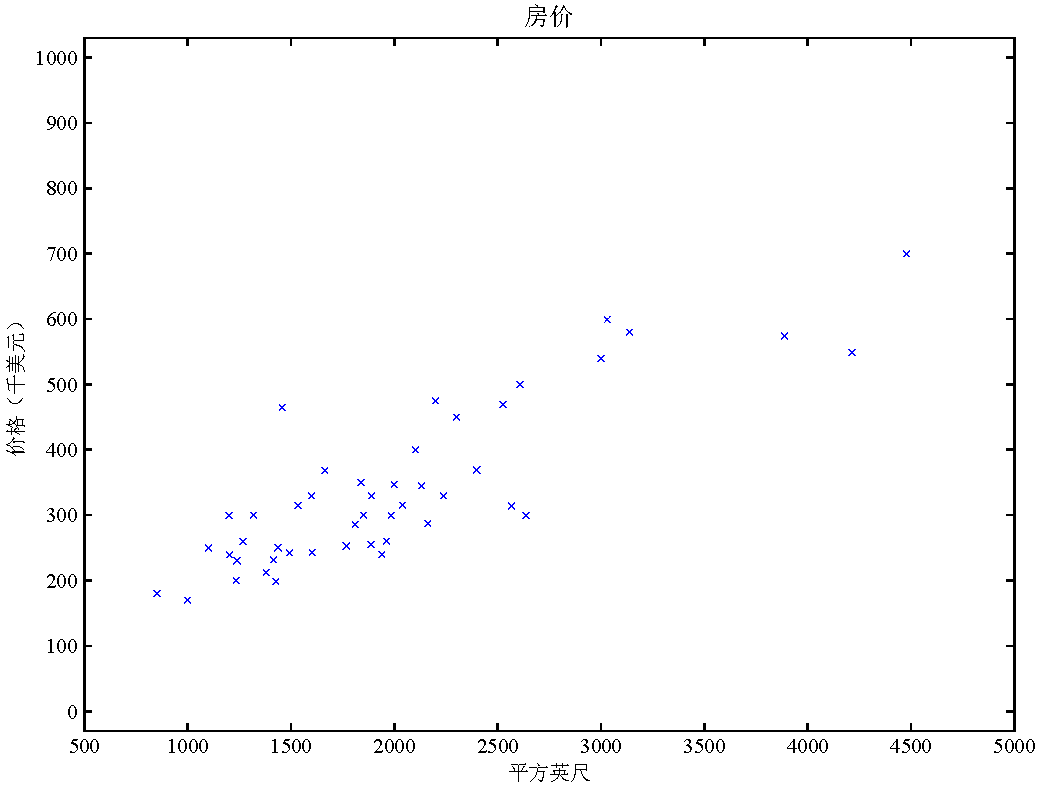
\includegraphics[width=0.5\linewidth]{figs/house_dataset_plot1.pdf}
\end{figure}

有了这些数据之后,该怎样根据波特兰其他房屋的居住面积来预测其价格呢?

为了后续使用的方便,在这里做如下约定。约定用 $x^{(i)}$ 表示“输入”变量(示例中是居住面积),也称作输入\textbf{特征 (features)};用 $y^{(i)}$ 表示要预测的“输出”或\textbf{目标 (target) }变量(价格)。一对 $(x^{(i)}, y^{(i)})$ 称为一个\textbf{训练样本 (training example)},而用于学习的数据集——由 $n$ 个训练样本组成的列表 $\{(x^{(i)}, y^{(i)}); i = 1,...,n\}$——则称为\textbf{训练集 (training set)}。注意,此处的上标“$i$”仅表示训练集中的索引,而不表示指数运算。此外,用 $\mathcal{X}$ 表示输入的取值空间,$\mathcal{Y}$ 表示输出的取值空间。在本例中,有 $\mathcal{X} = \mathcal{Y} = \mathbb{R}$。

监督学习问题可以更加形式化地表述为:给定一个训练集,目标是学习一个函数 $h: \mathcal{X} \mapsto \mathcal{Y}$,该函数能够对输入 $x$ 进行预测,使其输出 $h(x)$ 与“很好地”预测相应的真实值 $y$。出于历史原因,函数 $h$ 被称为 \textbf{假设 (hypothesis)}。整个过程如下图所示:

\begin{figure}[H]
\centering
\begin{tikzpicture}[node distance=2cm, auto]
    \node [rounded corners=1mm, rectangle, align=center, draw] (training) {训练集};
    \node [rounded corners=1mm, rectangle, align=center, draw, below of=training] (learning) {学习算法};
    \node [rounded corners=1mm, rectangle, align=center, draw, below of=learning] (h) {$h$};
    \node [left of=h, label={[align=center]below:\footnotesize (房屋居住面积)}] (x) {$x$};
    \node [right of=h, label={[align=center]below:\footnotesize (房屋预测价格)}] (y) {预测值 $y$};

    \path [->, draw] (training) -- (learning);
    \path [->, draw] (learning) -- (h);
    \path [->, draw] (x) -- (h);
    \path [->, draw] (h) -- (y);
\end{tikzpicture}
\end{figure}

当预测的目标变量是连续值时(例如预测房价),称这类学习问题为\textbf{回归 (regression)} 问题。当 $y$ 只能取有限个离散值时(例如根据居住面积预测住宅是房屋还是公寓),则称为\textbf{分类 (classification)} 问题。

\chapter{线性回归}

为了让上面的房屋示例更有趣,不妨考虑一个更为丰富的数据集。除了居住面积外,该数据集还包括了每栋房屋的卧室数量:

\begin{table}[H]
    \centering
    \begin{tabular}{c|c|c}
        居住面积 (平方英尺) & 卧室数 & 价格 (1000\$) \\
        \hline
        2104 & 3 & 400 \\
        1600 & 3 & 330 \\
        2400 & 3 & 369 \\
        1416 & 2 & 232 \\
        3000 & 4 & 540 \\
        $\vdots$ & $\vdots$ & $\vdots$
    \end{tabular}
    \label{tab:house_example2}
\end{table}

此处,$x$ 是 $\mathbb{R}^2$ 中的二维向量。对于训练集中第 $i$ 栋房屋,$x_1^{(i)}$ 是其居住面积,而 $x_2^{(i)}$ 是其卧室数量。(在设计学习问题时,特征的选择通常取决于你的具体需求。例如,在收集波特兰的房屋数据时,除了居住面积和卧室数量,还可以考虑纳入壁炉、浴室数量等其他特征。关于特征选择的深入讨论将在后续展开,目前先基于当前给定的两个特征进行分析。)

在进行监督学习时,需要明确如何在计算机中表示假设函数 $h$。不妨先尝试用 $x$ 的线性函数来近似 $y$:

\[
    h_\theta(x) = \theta_0 + \theta_1x_1 + \theta_2x_2
\]
在此处,$\theta_i$ 是该模型的\textbf{参数 (parameters)},亦称\textbf{权重 (weights)}。它们参数化了从特征空间 $\mathcal{X}$ 到目标空间 $\mathcal{Y}$ 的线性函数。在不引起混淆的前提下,可以省略 $h_\theta(x)$ 中的下标 $\theta$,直接写作 $h(x)$。为了进一步简化表示,我们引入约定:令 $x_0 = 1$。这个 $x_0$ 对应的系数 $\theta_0$ 通常被称为\textbf{截距项 (intercept term)}。这样就有

\[
    h(x) = \sum_{i=0}^d \theta_i x_i = \theta^T x,
\]
其中 $\theta$ 和 $x$ 视为向量,而 $d$ 则是输入变量的数量 (不计入 $x_0$)。

现在,对于给定的训练集,我们应该如何选择或学习参数 $\theta$ 呢?一个直观且合理的方法是,使假设函数 $h(x)$ 对于训练样本的输出 $h_\theta(x^{(i)})$ 尽可能地接近其对应的真实值 $y^{(i)}$。为了形式化地表述这个接近程度,我们定义一个函数,用于衡量对于任意给定的参数值 $\theta$,预测值 $h_\theta(x^{(i)})$ 与实际值 $y^{(i)}$ 之间的差异。这个函数被称为\textbf{代价函数 (cost function)}:

\[
    J(\theta) = \frac{1}{2} \sum_{i=1}^n (h_\theta(x^{(i)}) - y^{(i)})^2.
\]

熟悉线性回归的读者可能会发现,此处定义的函数即为\textbf{普通最小二乘 (ordinary least squares)} 回归模型所使用的最小二乘代价函数。但本讲义不要求读者具备相关背景知识,后文将对此进行详细阐述,并最终指出这仅是更广泛算法族中的一个特例。


\section{最小均方算法}

我们的目标是找到能够最小化代价函数 $J(\theta)$ 的参数 $\theta$。为此,我们可以考虑一种搜索算法:该算法从对 $\theta$ 的某个“初始猜测”开始,然后不断地调整 $\theta$ 的值,使其沿着使 $J(\theta)$ 减小的方向移动,直到最终收敛到最小化 $J(\theta)$ 的 $\theta$ 值。具体而言,我们考虑使用\textbf{梯度下降 (gradient descent)} 算法。该算法从某个初始的 $\theta$ 值开始,并重复执行以下更新步骤:

\[
    \theta_j := \theta_j - \alpha \frac{\partial}{\partial\theta_j} J(\theta).
\]
(上述更新操作同时应用于 $j = 0, \dots, d$ 的所有参数 $\theta_j$。)这里的 $\alpha$ 被称为\textbf{学习率 (learning rate)}。这是一种非常自然的算法:它每一步都沿着代价函数 $J$ 下降最快的方向进行更新。

为了实现上述算法,需要计算公式右侧的偏导数项。可以先考虑只有一个训练样本 $(x, y)$ 的情况,这样就可以暂时忽略代价函数 $J$ 定义中的求和操作。在这种情况下,偏导数计算如下:

\[
    \begin{aligned}
    \frac{\partial}{\partial\theta_j} J(\theta) &= \frac{\partial}{\partial\theta_j} \frac{1}{2} (h_\theta(x) - y)^2 \\
    &= 2 \cdot \frac{1}{2} (h_\theta(x) - y) \cdot \frac{\partial}{\partial\theta_j} (h_\theta(x) - y) \\
    &= (h_\theta(x) - y) \cdot \frac{\partial}{\partial\theta_j} \left( \sum_{i=0}^d \theta_i x_i - y \right) \\
    &= (h_\theta(x) - y) x_j
    \end{aligned}
\]

上式给出了针对单个训练样本的更新规则:\footnote{符号 “$a := b$” 用于表示(计算机程序中的)一个操作,其中变量 $a$ 的值被设置为 $b$。换句话说,这个操作用 $b$ 的值覆盖了 $a$ 的值。反之,如果需要断言 $a$ 的值等于 $b$ 的值,会写作 “$a = b$”。}

\[
    \theta_j := \theta_j + \alpha (y^{(i)} - h_\theta(x^{(i)})) x_j^{(i)}.
\]
这个规则被称为\textbf{最小均方 (Least mean squares, LMS)} 更新规则,也称为 \textbf{Widrow-Hoff} 学习规则。该规则具有一些自然而直观的特性。例如,更新的幅度与\textbf{误差 (error)} 项 $(y^{(i)} - h_\theta(x^{(i)}))$ 成正比;因此,如果对于一个训练样本,其预测值几乎等于 $y^{(i)}$ 的实际值,那么参数就几乎不需要调整;反之,如果预测的 $h_\theta(x^{(i)})$ 有很大的误差 (即与 $y^{(i)}$ 相差甚远),则需要对参数进行更大的调整。

所推导的 LMS 规则是针对只有一个训练样本的情况。要将其应用于包含多个样本的训练集,有两种常见的方法。第一种方法是将算法修改为以下形式:

\vspace{0.5em}
重复直到收敛 \{
\begin{equation}
    \theta_j := \theta_j + \alpha \sum_{i=1}^n (y^{(i)} - h_\theta(x^{(i)})) x_j^{(i)}, \text{(对于每个 } j) \label{eq:1.1}
\end{equation}
\indent\}
\vspace{0.5em}

将逐位置的更新向量化到 $\theta$,可以稍微简化 \eqref{eq:1.1}:

\[
    \theta := \theta + \alpha \sum_{i=1}^n (y^{(i)} - h_\theta(x^{(i)})) x^{(i)}
\]

读者不难验证,上述更新规则中求和项所表示的量,恰好对应于我们先前定义的成本函数的偏导数 $\partial J(\theta) / \partial \theta_j$。因此,这个更新规则实际上就是在原始成本函数 $J$ 上进行梯度下降。这种方法在每一步都利用了整个训练集的所有样本,因此被称为\textbf{批量梯度下降 (batch gradient descent)}。值得注意的是,尽管梯度下降算法在一般情况下可能收敛到局部最优解,但对于我们这里的线性回归问题,其优化目标函数 $J$ 具有良好的性质:它是一个凸二次函数。这意味着它只有一个全局最小值,没有其他局部最优解。因此,在合适的学习率 $\alpha$ 下,梯度下降算法能够保证收敛到全局最优解。下面是一个用梯度下降最小化一个二次函数的图例。

\begin{figure}[H]
    \centering
    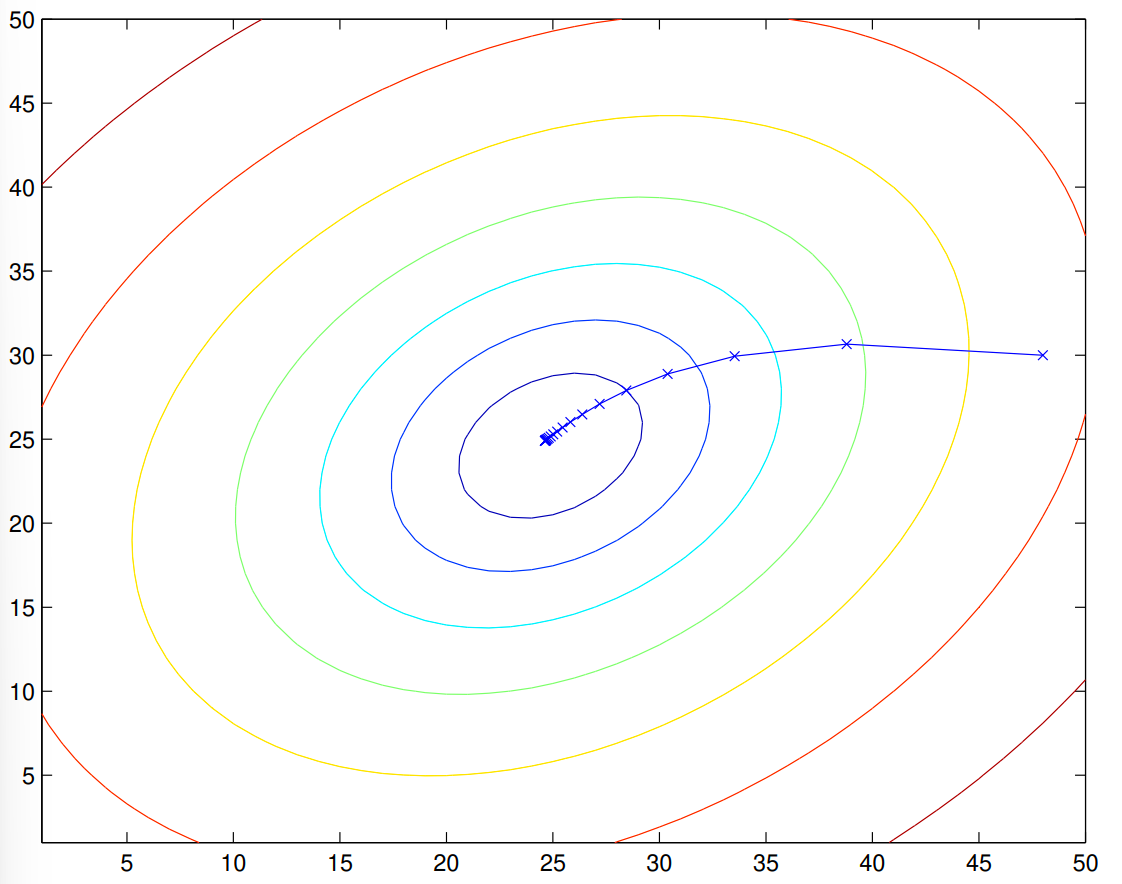
\includegraphics[width=0.5\linewidth]{figs/gradient_descent_trajectory.png}
    \label{fig:gradient_descent_trajectory}
\end{figure}
上面的椭圆是二次函数的等高线。图中还显示了梯度下降的轨迹,其初始化参数是 (48,30),而由直线连接的叉号 $\text{x}$ 则是梯度下降所经过的一系列参数 $\theta$ 值。

在之前的数据集上应用批量梯度下降算法来拟合参数 $\theta$,以学习根据居住面积预测房价的函数,最终得到的参数值为 $\theta_0 = 71.27$ 和 $\theta_1 = 0.1345$。将学习到的函数 $h_\theta(x)$,作为输入变量 $x$(表示居住面积)的函数,与训练数据一同绘制,结果如下图所示:

\begin{figure}[H]
    \centering
    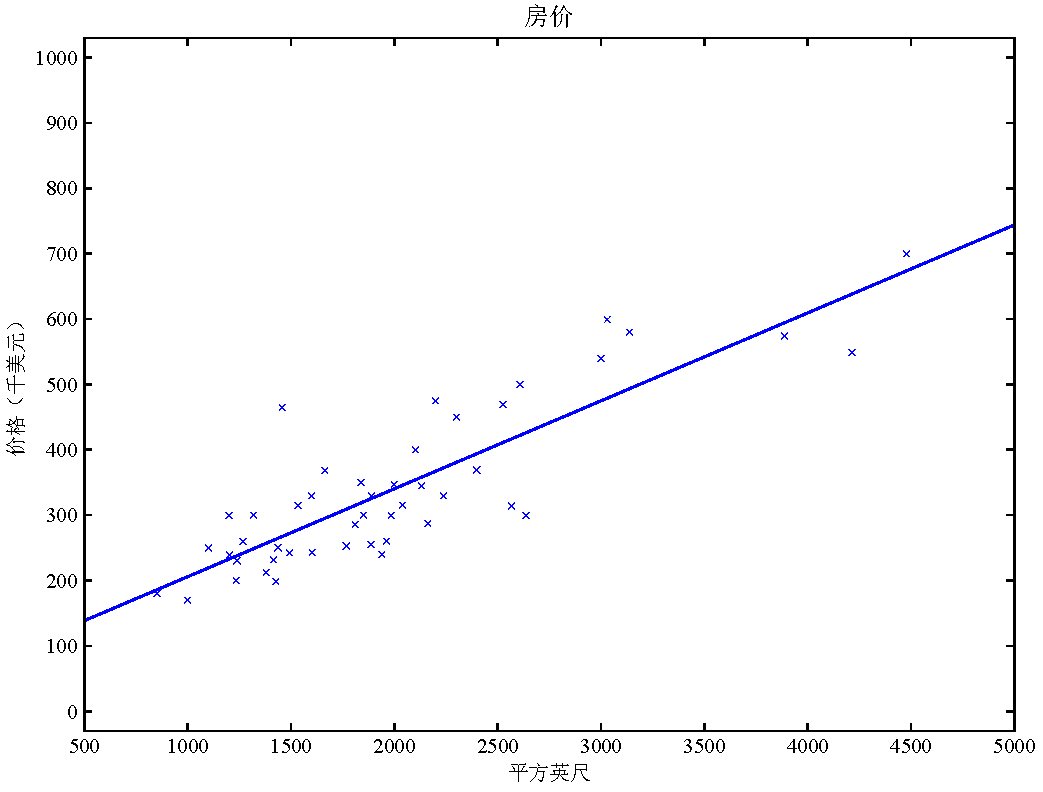
\includegraphics[width=0.5\linewidth]{figs/house_dataset_plot2.pdf}
\end{figure}
如果把卧室数量也当作输入特征,最终得到的参数值为 $\theta_0 = 89.60, \theta_1 = 0.1392, \theta_2 = -8.738$。

上述结果是通过批量梯度下降算法得到的。除此之外,还有一种很好的替代算法:

\vspace{0.5em}
循环 \{

$\quad\quad$对于 $i = 1$ 到 $n$,\{

\begin{equation}
    \theta_j := \theta_j + \alpha (y^{(i)} - h_\theta(x^{(i)})) x_j^{(i)}, \text{(对于每个 } j) \label{eq:1.2}
\end{equation}

$\quad\quad$\}

\indent\}
\vspace{0.5em}

将逐位置的更新向量化到 $\theta$,可以稍微简化 \eqref{eq:1.2}:

\[
    \theta := \theta + \alpha (y^{(i)} - h_\theta(x^{(i)})) x^{(i)}
\]

这种算法会重复遍历训练集,每次遇到一个训练样本时,仅针对该单个样本计算误差梯度并更新参数。这种方法被称为\textbf{随机梯度下降 (stochastic gradient descent)},有时也称为\textbf{增量梯度下降 (incremental gradient descent)}。与批量梯度下降不同,批量梯度下降在执行单次更新前需要扫描整个训练集(当训练集规模 $n$ 很大时,这是一项昂贵的操作),而随机梯度下降可以立即开始并对每个样本都取得进展。通常情况下,随机梯度下降能更快地使参数 $\theta$ “接近”最小值。(然而,需要注意的是,它可能不会完全“收敛”到最小值,参数 $\theta$ 可能会在目标函数 $J(\theta)$ 的最小值附近持续振荡。但在实际应用中,接近最小值的大多数值都足以作为真实最小值的良好近似。\footnote{通过在算法运行过程中缓慢地减小学习率 $\alpha$ 至零,可以确保参数收敛到全局最小值,而不仅仅是在最小值附近振荡。} )因此,特别是在训练集很大时,通常更倾向于使用随机梯度下降而非批量梯度下降。


\section{正规方程}

梯度下降提供了一种最小化目标函数 $J$ 的迭代方法。接下来,我们将探讨另一种无需迭代的最小化 $J$ 的方法。具体而言,我们将通过明确地计算 $J$ 关于每个参数 $\theta_j$ 的偏导数,并将这些导数置为零来求解最小值。为了避免繁琐的代数运算和大量的导数矩阵书写,我们将在下文引入一些矩阵微积分的记号。

\subsection{矩阵导数}

对于一个将 $n \times d$ 矩阵映射到实数的函数 $f: \mathbb{R}^{n \times d} \mapsto \mathbb{R}$,我们定义 $f$ 对 $A$ 的导数:

\[
    \nabla_A f(A) = \begin{bmatrix} 
        &\frac{\partial f}{\partial A_{11}} & \cdots & \frac{\partial f}{\partial A_{1d}} & \\ 
        &\vdots & \ddots & \vdots & \\ 
        &\frac{\partial f}{\partial A_{n1}} & \cdots & \frac{\partial f}{\partial A_{nd}} &
    \end{bmatrix}
\]

因此,梯度 $\nabla_A f(A)$ 本身是一个 $n \times d$ 矩阵,其 $(i, j)$ 元素是 $\partial f / \partial A_{ij}$。例如,假设 $A = \begin{bmatrix} & A_{11} & A_{12} & \\ & A_{21} & A_{22} & \end{bmatrix}$ 是一个 $2 \times 2$ 矩阵,并且函数 $f: \mathbb{R}^{2 \times 2} \mapsto \mathbb{R}$ 由下式给出

\[
    f(A) = \frac{3}{2} A_{11} + 5 A_{12}^2 + A_{21} A_{22}.
\]

这里,$A_{ij}$ 表示矩阵 $A$ 在 $(i, j)$ 位置上的元素。则可以得到

\[
    \nabla_A f(A) = \begin{bmatrix} & \frac{3}{2} & 10A_{12} & \\ & A_{22} & A_{21}& \end{bmatrix}.
\]

\subsection{再探最小二乘法}

掌握了矩阵导数的工具后,我们现在可以着手求解使目标函数 $J(\theta)$ 最小化的 $\theta$ 的闭式解。首先,我们用矩阵向量符号重写 $J$。

给定一个训练集,我们定义\textbf{设计矩阵 (design matrix)} $X$。这是一个 $n \times d$ 矩阵(如果包含截距项,则为 $n \times (d+1)$ 矩阵),其每一行对应一个训练样本的输入特征向量:

\[
    X = \begin{bmatrix} &- (x^{(1)})^T -& \\ &- (x^{(2)})^T -& \\ &\vdots& \\ &- (x^{(n)})^T -& \end{bmatrix}.
\]
进一步地,我们定义向量 $\vec{y}$,它是一个 $n$ 维列向量,其分量依次为训练集中各个样本的目标值:
\[
    \vec{y} = \begin{bmatrix} &y^{(1)}& \\ &y^{(2)}& \\ &\vdots& \\ &y^{(n)}& \end{bmatrix}.
\]
根据 $h_\theta(x^{(i)}) = (x^{(i)})^T \theta$,不难验证
\[
    \begin{aligned}
        X\theta - \vec{y} 
        &= \begin{bmatrix} &(x^{(1)})^T \theta& \\ &\vdots& \\ &(x^{(n)})^T \theta& \end{bmatrix} - \begin{bmatrix} &y^{(1)}& \\ &\vdots& \\ &y^{(n)}& \end{bmatrix} \\
        &= \begin{bmatrix} &h_\theta(x^{(1)}) - y^{(1)}& \\ &\vdots& \\ &h_\theta(x^{(n)}) - y^{(n)}& \end{bmatrix}.
    \end{aligned}
\]
利用向量 $z$ 满足 $z^T z = \sum_i z_i^2$ 这一性质,可以得到
\[
    \begin{aligned}
        \frac{1}{2}(X\theta - \vec{y})^T (X\theta - \vec{y}) 
        &= \frac{1}{2} \sum_{i=1}^n (h_\theta (x^{(i)}) - y^{(i)})^2 \\
        &= J(\theta)
    \end{aligned}
\]
最后,为了最小化 $J$,对其关于 $\theta$ 求导,得到:
\[
    \begin{aligned}
        \nabla_\theta J(\theta) &= \nabla_\theta \frac{1}{2} (X\theta - \vec{y})^T (X\theta - \vec{y}) \\
        &= \frac{1}{2} \nabla_\theta ((X\theta)^T X\theta - (X\theta)^T \vec{y} - \vec{y}^T (X\theta) + \vec{y}^T \vec{y}) \\
        &= \frac{1}{2} \nabla_\theta (\theta^T X^T X\theta - \theta^T X^T \vec{y} - \vec{y}^T X\theta) \\
        &= \frac{1}{2} \nabla_\theta (\theta^T X^T X\theta - 2(X^T \vec{y})^T \theta) \\
        &= \frac{1}{2} (2 X^T X\theta - 2 X^T \vec{y}) \\
        &= X^T X\theta - X^T \vec{y}
    \end{aligned}
\]
在上述推导中,第三步利用了向量内积的交换律 $a^T b = b^T a$;第五步则利用了向量求导公式 $\nabla_x b^T x = b$ 以及对于对称矩阵 $A$,$\nabla_x x^T A x = 2Ax$(详细推导可参考第 4.3 节的“线性代数回顾与参考”)。为了最小化 $J$,我们将上述导数设为零,从而得到\textbf{正规方程 (normal equations)}:
\[
    X^T X\theta = X^T \vec{y}
\]
因此,使 $J(\theta)$ 最小的 $\theta$ 的闭式解是
\[
    \theta = (X^T X)^{-1} X^T \vec{y}.\footnote{需要注意的是,上述推导隐式假设了 $X^T X$ 是一个可逆矩阵。在计算其逆矩阵之前,应先进行可逆性检查。当线性独立样本的数量少于特征数量,或者特征之间存在线性相关性时,$X^T X$ 将是不可逆的。即使在这种情况下,也可以通过其他技术来“修复”,但为了保持简洁,此处省略。}
\]


\section{概率解释}

在面对回归问题时,我们通常会采用线性回归模型,并以最小化平方误差和(即最小二乘代价函数 $J$)作为学习目标。本节旨在解释为什么这种方法是合理的,并将阐明在哪些特定的概率假设下,最小二乘回归可以自然地从概率模型中推导出来。

假设目标变量与输入变量之间的关系可以通过以下方程进行建模:
\[
    y^{(i)} = \theta^T x^{(i)} + \epsilon^{(i)},
\]
此处 $\epsilon^{(i)}$ 表示一个误差项,它包含了模型中未建模的因素(例如,一些对预测结果有显著影响但未纳入模型的特征)以及固有的随机噪声。我们进一步假定这些误差项 $\epsilon^{(i)}$ 是独立同分布 (IID) 的,并且都服从均值为零、方差为 $\sigma^2$ 的高斯分布(也称为正态分布),写作 “$\epsilon^{(i)} \sim \mathcal{N}(0, \sigma^2)$”。由此,$\epsilon^{(i)}$ 的概率密度函数可以写为:
\[
    p(\epsilon^{(i)}) = \frac{1}{\sqrt{2\pi}\sigma} \exp\left(-\frac{(\epsilon^{(i)})^2}{2\sigma^2}\right).
\]
这意味着
\[
    p(y^{(i)} | x^{(i)}; \theta) = \frac{1}{\sqrt{2\pi}\sigma} \exp\left(-\frac{(y^{(i)} - \theta^T x^{(i)})^2}{2\sigma^2}\right).
\]
符号 “$p(y^{(i)} | x^{(i)}; \theta)$” 表示这是给定 $x^{(i)}$ 的条件下,由 $\theta$ 参数化的 $y^{(i)}$ 的分布。需要注意的是,我们不应该将 $\theta$ 作为条件(即写成“$p(y^{(i)} | x^{(i)}, \theta)$”),因为这里 $\theta$ 被视为一个未知但固定的值,而非一个随机变量。此外,也可以将 $y^{(i)}$ 的分布写成 $y^{(i)} | x^{(i)}; \theta \sim \mathcal{N}(\theta^T x^{(i)}, \sigma^2)$。

给定设计矩阵 $X$(包含所有输入向量 $x^{(i)}$)和参数 $\theta$,我们就可以确定每个观测值 $y^{(i)}$ 的条件分布。因此,整个数据集的概率可以表示为 $p(\vec{y} | X; \theta)$ 。当我们将 $\theta$ 视为固定值时,这个概率是关于观测数据 $\vec{y}$(可能还有 $X$)的函数。然而,在推断模型参数时,我们更关注的是在给定观测数据 $\vec{y}$ 和输入数据 $X$ 的情况下,不同参数值 $\theta$ 的可能性。此时,我们将 $p(\vec{y} | X; \theta)$ 视为关于 $\theta$ 的函数,并称之为\textbf{似然函数 (likelihood function)}:
\[
    L(\theta) = L(\theta; X, \vec{y}) = p(\vec{y} | X; \theta).
\]
需要注意的是,根据 $\epsilon^{(i)}$ 的独立性假设(这隐含了在给定 $x^{(i)}$ 条件下 $y^{(i)}$ 的独立性),上式也可以写成
\[
    \begin{aligned}
        L(\theta) &= \prod_{i=1}^n p(y^{(i)} | x^{(i)}; \theta) \\
        &= \prod_{i=1}^n \frac{1}{\sqrt{2\pi}\sigma} \exp\left(-\frac{(y^{(i)} - \theta^T x^{(i)})^2}{2\sigma^2}\right).
    \end{aligned}
\]

现在,给定这个描述 $y^{(i)}$ 和 $x^{(i)}$ 之间关系的概率模型,我们应该怎么得到最优的参数 $\theta$?\textbf{最大似然 (maximum likelihood)} 原理表明,应该选能使观测数据出现的概率尽可能高的参数 $\theta$。换句话说,我们应该选择能够最大化似然函数 $L(\theta)$ 的 $\theta$ 值。

最大化 $L(\theta)$ 等价于最大化 $L(\theta)$ 的任何严格递增函数。特别地,如果选择最大化\textbf{对数似然 (log likelihood)} $\ell(\theta)$,推导过程会更加简化:
\[
    \begin{aligned}
    \ell(\theta) &= \log L(\theta) \\
    &= \log \prod_{i=1}^n \frac{1}{\sqrt{2\pi}\sigma} \exp\left(-\frac{(y^{(i)} - \theta^T x^{(i)})^2}{2\sigma^2}\right) \\
    &= \sum_{i=1}^n \log \frac{1}{\sqrt{2\pi}\sigma} \exp\left(-\frac{(y^{(i)} - \theta^T x^{(i)})^2}{2\sigma^2}\right) \\
    &= \sum_{i=1}^n \left(\log \frac{1}{\sqrt{2\pi}\sigma} - \frac{(y^{(i)} - \theta^T x^{(i)})^2}{2\sigma^2}\right) \\
    &= n \log \frac{1}{\sqrt{2\pi}\sigma} - \frac{1}{2\sigma^2} \sum_{i=1}^n (y^{(i)} - \theta^T x^{(i)})^2.
    \end{aligned}
\]
因此,最大化 $\ell(\theta)$ 与最小化
\[
    \frac{1}{2} \sum_{i=1}^n (y^{(i)} - \theta^T x^{(i)})^2,
\]
结果相同,而这正是 $J(\theta)$,也即最初的最小二乘代价函数。

总结来说,在我们先前对数据分布做出的概率假设下,最小二乘回归实际上对应于求解参数 $\theta$ 的最大似然估计。因此,这些概率假设构成了一组能够证明最小二乘回归是一种非常自然的最大似然估计方法的条件。(然而需要注意的是,这些概率假设并非使得最小二乘回归成为一个合理有效方法的必要条件,事实上也存在其他自然的假设能够证明其合理性。)

另外需要指出的是,在之前的推导中,对参数 $\theta$ 的最终选择并不依赖于 $\sigma^2$ 的具体数值,即使 $\sigma^2$ 未知,我们也能得到相同的结果。这一特性在后续讨论指数族和广义线性模型时将会再次得到利用。


\section{局部加权线性回归(选读)}

考虑从 $x \in \mathbb{R}$ 预测 $y$ 的问题。下图最左边的图显示了将 $y = \theta_0 + \theta_1x$ 拟合到数据集的结果。从图中可以看出,这些数据点并未完全落在一条直线上,因此拟合效果并不理想。

\begin{figure}[H]
  \centering
  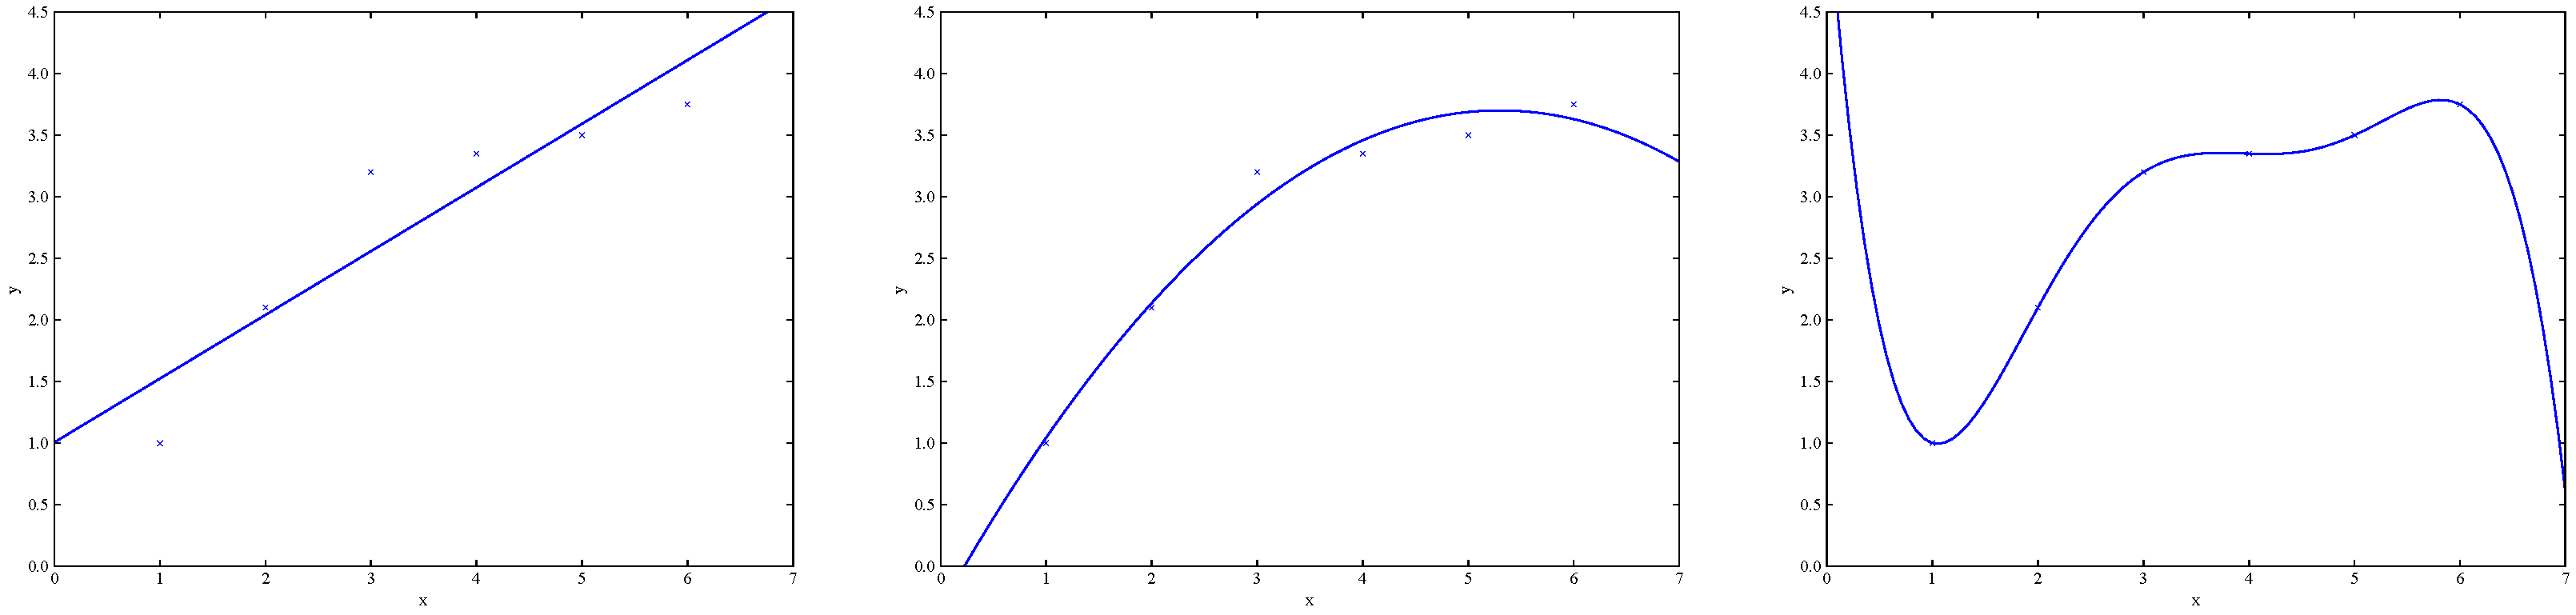
\includegraphics[width=0.93\linewidth]{figs/regression_plot.pdf}
\end{figure}

作为对比,如果我们添加一个额外的特征 $x^2$,然后拟合模型 $y = \theta_0 + \theta_1 x + \theta_2 x^2$,那么对数据的拟合效果可能会有所改善(参见中间图)。有人可能会简单地认为添加的特征越多越好。然而,过度添加特征也存在风险:最右边的图展示了拟合一个五阶多项式 $y = \sum_{j=0}^5 \theta_j x^j$ 的结果。尽管这条拟合曲线完美地穿过了所有数据点,我们也不能期望它能很好地预测不同居住区域 ($x$) 的房价 ($y$)。非正式地借用一下拟合的术语,可以说左边的图是\textbf{欠拟合 (underfitting)} 的一个例子——模型未能捕捉到数据中明显的结构——而右边的图则是一个\textbf{过拟合 (overfitting)} 的例子。(在课程后续的学习理论部分,我们将正式定义这些概念,并更严谨地探讨判断一个假设优劣的标准。)

正如先前讨论的,特征的选择对于确保学习算法的良好性能至关重要。(在后续关于模型选择的讨论中,我们也会介绍一些能够自动选择合适特征的算法。)在本节中,我们将简要介绍局部加权线性回归 (locally weighted linear regression, LWR) 算法。该算法假设有足够的训练数据,使得特征的选择不那么关键。鉴于读者将在作业中自行探索 LWR 算法的一些特性,本节的讲解将较为简略。

在原始的线性回归算法中,为了使用输入 $x$ 进行预测(即计算 $h(x)$ 的值),通常需要执行以下步骤:

\begin{enumerate}
    \item 拟合 $\theta$ 以最小化 $\sum_i (y^{(i)} - \theta^T x^{(i)})^2$。
    \item 输出 $\theta^T x$。
\end{enumerate}

相比之下,局部加权线性回归算法执行以下步骤:

\begin{enumerate}
    \item 拟合 $\theta$ 以最小化 $\sum_i w^{(i)} (y^{(i)} - \theta^T x^{(i)})^2$。
    \item 输出 $\theta^T x$。
\end{enumerate}

这里,$w^{(i)}$ 是非负的\textbf{权重 (weights)}。直观上,对于特定的训练样本 $i$,如果 $w^{(i)}$ 较大,则在确定参数 $\theta$ 时,模型会更倾向于使 $(y^{(i)} - \theta^T x^{(i)})^2$ 误差项尽可能小。反之,如果 $w^{(i)}$ 较小,则该误差项在拟合过程中基本上会被忽略。

一种常用的权重选择方法是\footnote{如果 $x$ 是向量,则推广为 $w^{(i)} = \exp(-(x^{(i)} - x)^T (x^{(i)} - x) / (2\tau^2))$,或者 $w^{(i)} = \exp(-(x^{(i)} - x)^T \Sigma^{-1} (x^{(i)} - x) / (2\tau^2))$,其中 $\tau$ 和 $\Sigma$ 需要选择合适的值。}
\[
    w^{(i)} = \exp\left(-\frac{(x^{(i)} - x)^2}{2\tau^2}\right).
\]
需要注意的是,权重取决于要评估的特定点 $x$。此外,如果 $|x^{(i)} - x|$ 的值很小,则 $w^{(i)}$ 接近 1;如果 $|x^{(i)} - x|$ 的值很大,则 $w^{(i)}$ 会很小。因此,在选择 $\theta$ 时,靠近查询点 $x$ 的训练样本(即其误差项 $y^{(i)} - \theta^T x^{(i)}$)会被赋予更高的“权重”。(另外需要说明的是,尽管权重的表达式形式上类似于高斯分布的概率密度函数,但 $w^{(i)}$ 与高斯分布并没有直接联系,特别是 $w^{(i)}$ 并非随机变量,无论是正态分布还是其他分布。)参数 $\tau$ 控制着训练样本的权重随其与查询点 $x$ 距离衰减的速度;$\tau$ 被称为\textbf{带宽 (bandwidth)} 参数,这也是在作业中需要进行实验的内容。

局部加权线性回归是我们遇到的第一个\textbf{非参数 (non-parametric)} 算法示例。之前讨论的(无权重)线性回归算法被称为\textbf{参数化 (parametric)} 学习算法,因为它通过固定数量的参数($\theta_i$)来拟合数据。一旦这些参数 $\theta_i$ 被确定并存储下来,就不再需要保留训练数据来进行后续的预测。相比之下,为了使用局部加权线性回归进行预测,必须保留整个训练集。术语“非参数”(大致)反映了这样一个事实:表示假设函数 $h$ 所需存储的数据量与训练集的大小呈线性关系。

\chapter{分类与逻辑回归}

现在我们转向分类问题。这与回归问题类似,主要区别在于需要预测的目标变量 $y$ 只能取有限的离散值。目前,我们将重点讨论二元分类 (binary classification) 问题,其中 $y$ 的取值仅限于 0 和 1。(这里讨论的大部分内容也适用于多类别分类情况。)例如,在构建垃圾邮件分类器时,$x^{(i)}$ 可以代表一封电子邮件的某些特征,而 $y$ 则表示该邮件是否为垃圾邮件(垃圾邮件为 1,非垃圾邮件为 0)。通常,0 被称为\textbf{负类 (negetive class)},1 被称为\textbf{正类 (positive class)},有时也用符号 “$-$” 和 “$+$” 表示。对于给定的输入特征 $x^{(i)}$,其对应的 $y^{(i)}$ 被称为该训练样本的\textbf{标签 (label)}。

\section{逻辑回归}\label{sec:2.1}

在处理分类问题时,我们可以暂时忽略目标变量 $y$ 是离散值这一特性,并沿用之前的线性回归算法来尝试预测给定输入 $x$ 的 $y$ 值。然而,很容易构造出这种方法表现极差的例子。直觉上,由于 $y$ 只能取 $\{0, 1\}$ 中的值,模型的输出 $h_\theta(x)$ 取大于 1 或小于 0 的值是没有意义的。为了解决这一问题,我们需要改变假设函数 $h_\theta(x)$ 的形式。具体而言,我们将选择:
\[
    h_\theta(x) = g(\theta^T x) = \frac{1}{1+e^{-\theta^T x}},
\]
其中
\[
    g(z) = \frac{1}{1+e^{-z}}.
\]
称为\textbf{逻辑函数 (logistic function)} 或 \textbf{S 形函数 (sigmoid function)}。下面是 $g(z)$ 的图像:

\begin{figure}[H]
    \centering
    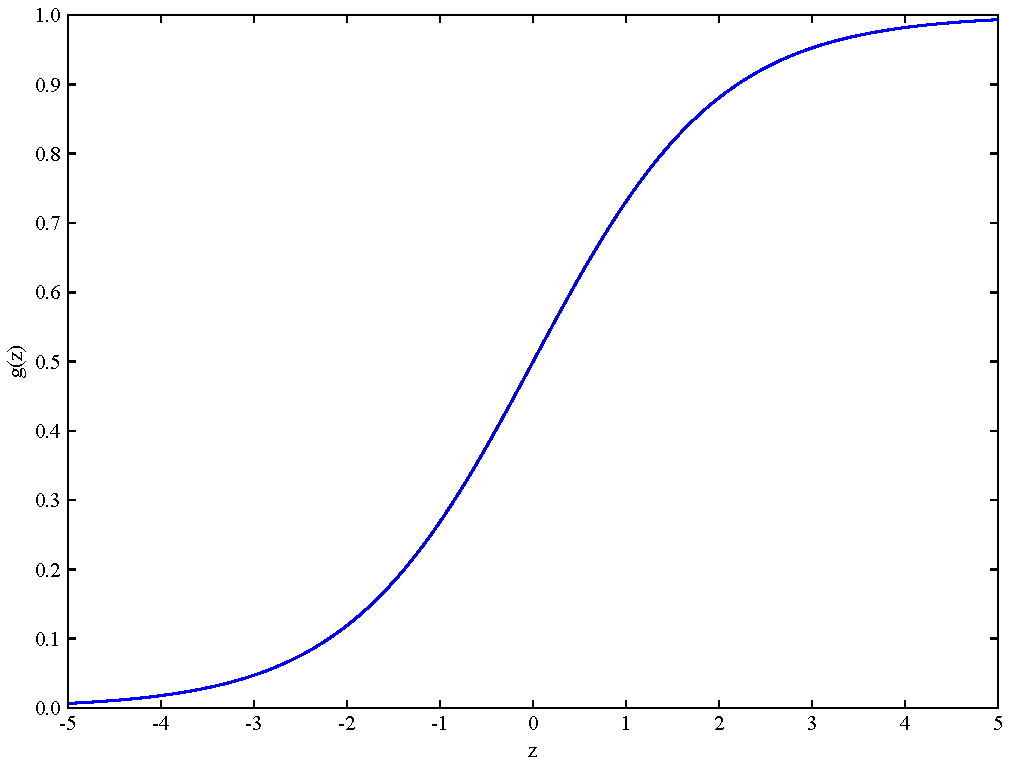
\includegraphics[width=0.5\linewidth]{figs/sigmoid.pdf}
    \label{fig:sigmoid}
\end{figure}

注意到 $g(z)$ 在 $z \to \infty$ 时趋于 1,在 $z \to -\infty$ 时趋于 0。此外,$g(z)$,因此 $h(x)$,始终介于 0 和 1 之间。和之前一样,这里约定 $x_0 = 1$,从而有 $\theta^T x = \theta_0 + \sum_{j=1}^d \theta_j x_j$。

现在先将 $g$ 的形式视为一个已知条件。其他从 0 平滑增加到 1 的函数也可以使用,但出于一些原因(稍后讨论广义线性模型(GLMs)和生成学习算法时会看到),选择 sigmoid 函数是相当自然的。在进一步展开之前,这里给出 sigmoid 函数导数的一个有用性质,记为 $g'$:
\[
    \begin{aligned}
        g'(z) &= \frac{d}{dz} \frac{1}{1+e^{-z}} \\ 
        &= \frac{1}{(1+e^{-z})^2} (e^{-z}) \\ 
        &= \frac{1}{1+e^{-z}} \cdot \left(1 - \frac{1}{1+e^{-z}}\right) \\ 
        &= g(z)(1 - g(z)).
    \end{aligned}
\]

那么,给定这样的逻辑回归模型,我们如何为其拟合 $\theta$ 呢?参照我们之前所见,最小二乘回归在一定假设下可以作为最大似然估计的一种形式。因此,我们也将为分类模型设定一组概率假设,然后通过最大似然估计的方式来拟合参数。

假设
\[
    \begin{aligned}
        P(y=1 \mid x; \theta) &= h_\theta(x) \\
        P(y=0 \mid x; \theta) &= 1 - h_\theta(x)
    \end{aligned}
\]
注意到上述两个概率表达式可以合并为一个更紧凑的形式
\[
    p(y \mid x; \theta) = (h_\theta(x))^y (1 - h_\theta(x))^{1-y}
\]
假设 $n$ 个训练样本是独立生成的,那么参数的似然可以写成
\[
    \begin{aligned}
        L(\theta) &= p(\vec{y} \mid X; \theta) \\ 
        &= \prod_{i=1}^n p(y^{(i)} \mid x^{(i)}; \theta) \\ 
        &= \prod_{i=1}^n (h_\theta(x^{(i)}))^{y^{(i)}} (1 - h_\theta(x^{(i)}))^{1-y^{(i)}}
    \end{aligned}
\]
和之前一样,最大化对数似然会更容易推导:
\begin{equation}
    \ell(\theta) = \log L(\theta) = \sum_{i=1}^n y^{(i)} \log h(x^{(i)}) + (1 - y^{(i)}) \log(1 - h(x^{(i)}))
    \label{eq:logistic_log_likelihood}
\end{equation}

那么,如何最大化这个似然函数呢呢?类似于线性回归的推导过程,我们可以采用梯度上升法。以向量形式表示,参数的更新规则为 $\theta := \theta + \alpha \nabla_\theta \ell(\theta)$。(注意更新公式中的正号,因为现在是在最大化函数,而不是最小化函数。)接下来,我们将从一个训练样本 $(x, y)$ 出发,推导随机梯度上升规则的导数:

\begin{align}
    \frac{\partial}{\partial \theta_j} \ell(\theta) &= \left(y \frac{1}{g(\theta^T x)} - (1-y) \frac{1}{1-g(\theta^T x)}\right) \frac{\partial}{\partial \theta_j} g(\theta^T x) \notag\\ 
    &= \left(y \frac{1}{g(\theta^T x)} - (1-y) \frac{1}{1-g(\theta^T x)}\right) g(\theta^T x)(1-g(\theta^T x)) \frac{\partial}{\partial \theta_j} \theta^T x \notag\\ 
    &= (y(1-g(\theta^T x)) - (1-y)g(\theta^T x)) x_j \notag\\
    &= (y - g(\theta^T x)) x_j \label{eq:partial_loss_theta}
\end{align}

上面的推导利用了 $g'(z) = g(z)(1-g(z))$ 这一点。这给出了随机梯度上升规则:
\[
    \theta_j := \theta_j + \alpha (y^{(i)} - h_\theta(x^{(i)})) x_j^{(i)}
\]
如果将推导出的逻辑回归更新规则与最小均方更新规则进行比较,会发现它们在形式上是相同的;但这并不是同一个算法,因为这里的 $h_\theta(x^{(i)})$ 是 $\theta^T x^{(i)}$ 的非线性函数。尽管如此,对于一个截然不同的算法和学习问题,却得到了相同的更新规则,这确实有些令人惊讶。这仅仅是巧合吗?抑或是背后存在更深层的原因?我们将在讨论广义线性模型(GLM)时解答这个问题。

\begin{remark}\label{remark:2.1.1}
    同一个损失函数的另一种表示方式也很有用,特别是在第 \ref{sec:7.1} 节研究非线性模型时。
\end{remark}
\noindent 设逻辑损失函数 $\ell_{\text{logistic}}: \mathbb{R} \times \{0, 1\} \to \mathbb{R}_{\ge 0}$ 定义为
\begin{equation}
    \ell_{\text{logistic}}(t, y) \triangleq y \log(1 + \exp(-t)) + (1 - y) \log(1 + \exp(t)).
\end{equation}
通过代入 $h_\theta(x) = 1/(1 + e^{-\theta^T x})$,可以验证负对数似然(方程 \eqref{eq:logistic_log_likelihood} 中 $\ell(\theta)$ 的负值)可以改写为
\begin{equation}
    -\ell(\theta) = \ell_{\text{logistic}}(\theta^T x, y).
\end{equation}
通常 $\theta^T x$ 或 $t$ 称为 \textit{logit}。稍作运算可得
\begin{align}
    \frac{\partial \ell_{\text{logistic}}(t, y)}{\partial t} &= y \frac{-\exp(-t)}{1 + \exp(-t)} + (1 - y) \frac{1}{1 + \exp(-t)} \\ 
    &= \frac{1}{1 + \exp(-t)} - y. \label{eq:2.6}
\end{align}
然后,使用链式法则,得到
\begin{align}
    \frac{\partial}{\partial \theta_j} \ell(\theta) &= - \frac{\partial \ell_{\text{logistic}}(t, y)}{\partial t} \cdot \frac{\partial t}{\partial \theta_j} \\ 
    &= (y-1/(1+\exp(-t))) \cdot x_j = (y - h_\theta(x)) x_j, 
\end{align}
这与方程 \eqref{eq:partial_loss_theta} 的推导是一致的。在第 \ref{sec:7.1} 节中,会看到这种观点可以扩展到非线性模型。

\section{离题:感知器学习算法}

现在,我们将简要讨论一个具有历史意义的算法,该算法在后续讨论学习理论时也将再次被提及。考虑对逻辑回归方法进行修改,“强制”其输出值为 0 或 1。为此,一个自然而然的想法是将函数 $g$ 的定义改为阈值函数:
\[
    g(z) = 
    \begin{cases} 
        1 & \text{若 } z \ge 0 \\
        0 & \text{若 } z < 0 
    \end{cases}
\]
如果像之前一样令 $h_\theta(x) = g(\theta^T x)$,但使用上述修改后的 $g$ 定义,并且使用更新规则
\[
    \theta_j := \theta_j + \alpha (y^{(i)} - h_\theta(x^{(i)})) x_j^{(i)}.
\]
那么就得到了\textbf{感知机学习算法 (perceptron learning algorithm)}。

在 20 世纪 60 年代,有人认为“感知机”是脑中单个神经元如何工作的一个粗略模型。考虑到该算法的简单性,在讨论学习理论时,它也将为分析提供一个起点。然而,请注意,尽管感知机看起来与其他讨论过的算法相似,但它实际上与逻辑回归和最小二乘线性回归是完全不同类型的算法;特别是,很难从概率角度解释感知机的预测结果,或者将感知机推导为最大似然估计算法。


\section{多类别分类}\label{sec:2.3}

考虑一个分类问题,其中响应变量 $y$ 可以取 $k$ 个值中的任意一个,即 $y \in \{1, 2, \dots, k\}$。例如,除了将电子邮件分为垃圾邮件或非垃圾邮件这两类(这是一个二元分类问题),也可能希望将其分为三类,例如垃圾邮件、个人邮件和工作相关邮件。标签/响应变量仍然是离散的,但现在可以取超过两个值。因此,将它建模为服从多项分布。

在这种情况下,$p(y \mid x; \theta)$ 是关于 $k$ 个可能的离散结果的分布,因此是多项分布。回想一下,多项分布涉及 $k$ 个数 $\phi_1, \dots, \phi_k$,它们指定了每个结果的概率。注意,这些数必须满足 $\sum_{i=1}^k \phi_i = 1$。将设计一个参数化模型,该模型输出满足此约束的 $\phi_1, \dots, \phi_k$,给定输入 $x$。

引入 $k$ 组参数 $\theta_1, \dots, \theta_k$,每组参数都是 $\mathbb{R}^d$ 中的一个向量。直观地,希望使用 $\theta_1^T x, \dots, \theta_k^T x$ 来表示$\phi_1, \dots, \phi_k$,即概率 $P(y = 1 \mid x; \theta), \dots, P(y = k \mid x; \theta)$。然而,这种直接方法存在两个问题。首先,$\theta_j^T x$ 不一定在 $[0, 1]$ 范围内。其次,$\theta_j^T x$ 的总和不一定为 1。因此,将使用 softmax 函数将 $(\theta_1^T x, \dots, \theta_k^T x)$ 转换为一个非负且总和为 1 的概率向量。

定义函数 $\text{softmax}: \mathbb{R}^k \to \mathbb{R}^k$ 如下:
\begin{equation}
    \text{softmax}(t_1, \dots, t_k) = 
    \begin{bmatrix} 
        \frac{\exp(t_1)}{\sum_{j=1}^k \exp(t_j)} \\
        \vdots \\
        \frac{\exp(t_k)}{\sum_{j=1}^k \exp(t_j)}
    \end{bmatrix}.
\end{equation}
softmax 函数的输入,即这里的向量 $t$,通常被称为 \textit{logits}。注意,根据定义,softmax 函数的输出始终是一个概率向量,其分量非负且总和为 1。

令 $(t_1, \dots, t_k) = (\theta_1^T x, \dots, \theta_k^T x)$。将 softmax 函数应用于 $(t_1, \dots, t_k)$,并将输出用作概率 $P(y = 1 \mid x; \theta), \dots, P(y = k \mid x; \theta)$。得到以下概率模型:
\begin{equation}
    \begin{bmatrix} 
        P(y = 1 \mid x; \theta) \\
        \vdots& \\
        P(y = k \mid x; \theta)
    \end{bmatrix} =
    \text{softmax}(t_1, \dots, t_k) = 
    \begin{bmatrix} 
    &\frac{\exp(\theta_1^T x)}{\sum_{j=1}^k \exp(\theta_j^T x)}& \\
    &\vdots& \\
    &\frac{\exp(\theta_k^T x)}{\sum_{j=1}^k \exp(\theta_j^T x)}&
    \end{bmatrix}.
\end{equation}
为了符号上的方便,令 $\phi_i = \frac{\exp(t_i)}{\sum_{j=1}^k \exp(t_j)}$。更简洁地,上面的方程可以写成:
\begin{equation}
    P(y = i \mid x; \theta) = \phi_i = \frac{\exp(t_i)}{\sum_{j=1}^k \exp(t_j)} = \frac{\exp(\theta_i^T x)}{\sum_{j=1}^k \exp(\theta_j^T x)}.
\end{equation}
接下来,计算单个样本 $(x, y)$ 的负对数似然。
\begin{equation}
    -\log p(y \mid x, \theta) = -\log\left(\frac{\exp(t_y)}{\sum_{j=1}^k \exp(t_j)}\right) = -\log\left(\frac{\exp(\theta_y^T x)}{\sum_{j=1}^k \exp(\theta_j^T x)}\right).
\end{equation}
因此,损失函数,即训练数据的负对数似然,由下式给出:
\begin{equation}
    \ell(\theta) = \sum_{i=1}^n -\log\left(\frac{\exp(\theta_{y^{(i)}}^T x^{(i)})}{\sum_{j=1}^k \exp(\theta_j^T x^{(i)})}\right).
    \label{eq:multiclass_loss}
\end{equation}
定义交叉熵损失 $\ell_{\text{ce}}: \mathbb{R}^k \times \{1, \dots, k\} \to \mathbb{R}_{\ge 0}$ 是很方便的,它将上述复杂的方程模块化为\footnote{这里命名存在一些歧义。有些人将交叉熵损失定义为将概率向量(在本讲义中用 $\phi$ 表示)和标签 $y$ 映射到实数的函数,并将本讲义中的交叉熵损失称为 softmax-交叉熵损失。本讲义选择当前的命名约定是因为它与大多数现代深度学习库(如 PyTorch 和 Jax)的命名一致。}:
\begin{equation}
    \ell_{\text{ce}}((t_1, \dots, t_k), y) = -\log \left( \frac{\exp(t_y)}{\sum_{j=1}^k \exp(t_j)} \right).
\end{equation}
使用此记号,方程 \eqref{eq:multiclass_loss} 可以简写为:
\begin{equation}
    \ell(\theta) = \sum_{i=1}^n \ell_{\text{ce}}((\theta_1^\top x^{(i)}, \dots, \theta_k^\top x^{(i)}), y^{(i)}).
\end{equation}
此外,交叉熵损失的梯度也很便于推导。令 $t = (t_1, \dots, t_k)$,并回顾 $\phi_i = \frac{\exp(t_i)}{\sum_{j=1}^k \exp(t_j)}$。可以推导出:
\begin{equation}
    \frac{\partial \ell_{\text{ce}}(t, y)}{\partial t_i} = \phi_i - {1}\{y=i\},
\end{equation}
其中 ${1}\{\cdot\}$ 是指示函数,即当 $y=i$ 时 ${1}\{y=i\} = 1$,当 $y \ne i$ 时 $\{y=i\} = 0$。向量化形式如下,这对于第 \ref{chapter:7} 章将很有用:
\begin{equation}
    \frac{\partial \ell_{\text{ce}}(t, y)}{\partial t} = \phi - e_y,\label{eq:2.17}
\end{equation}
其中 $e_s \in \mathbb{R}^k$ 是第 $s$ 个标准基向量(其中第 $s$ 个分量是 1,其余所有分量都是零)。使用链式法则,有:
\begin{equation}
    \frac{\partial \ell_{\text{ce}}((\theta_1^\top x, \dots, \theta_k^\top x), y)}{\partial \theta_i} = \frac{\partial \ell(t, y)}{\partial t_i} \frac{\partial t_i}{\partial \theta_i} = (\phi_i - {1}\{y=i\}) \cdot x.
\end{equation}
因此,损失函数关于参数 $\theta_i$ 的梯度为:
\begin{equation}
    \frac{\partial \ell(\theta)}{\partial \theta_i} = \sum_{j=1}^n (\phi_i^{(j)} - {1}\{y^{(j)}=i\}) \cdot x^{(j)},
\end{equation}
其中 $\phi_i^{(j)} = \frac{\exp(\theta_i^\top x^{(j)})}{\sum_{s=1}^k \exp(\theta_s^\top x^{(j)})}$ 是模型预测样本 $x^{(j)}$ 属于类别 $i$ 的概率。利用上述梯度,可以使用(随机)梯度下降来最小化损失函数 $\ell(\theta)$。

\section{最大化 \texorpdfstring{$\ell(\theta)$}{l(theta)} 的另一种算法}

回到以 sigmoid 为 $g(z)$ 函数的逻辑回归,现在讨论一种不同的最大化 $\ell(\theta)$ 的算法。

首先,考虑牛顿法用于寻找函数零点。具体来说,假设有一个函数 $f: \mathbb{R} \to \mathbb{R}$,并且希望找到一个 $\theta$ 值使得 $f(\theta) = 0$。这里 $\theta \in \mathbb{R}$ 是一个实数。牛顿法执行以下更新:
\[
    \theta := \theta - \frac{f(\theta)}{f'(\theta)}.
\]
这种方法有一种自然的解释:将函数 $f$ 通过其在当前猜测值 $\theta$ 处的切线进行近似,然后求解该切线等于零的点,并将该点作为 $\theta$ 的下一个猜测值。

以下是牛顿法实际应用的图示:

\begin{figure}[H]
  \centering
  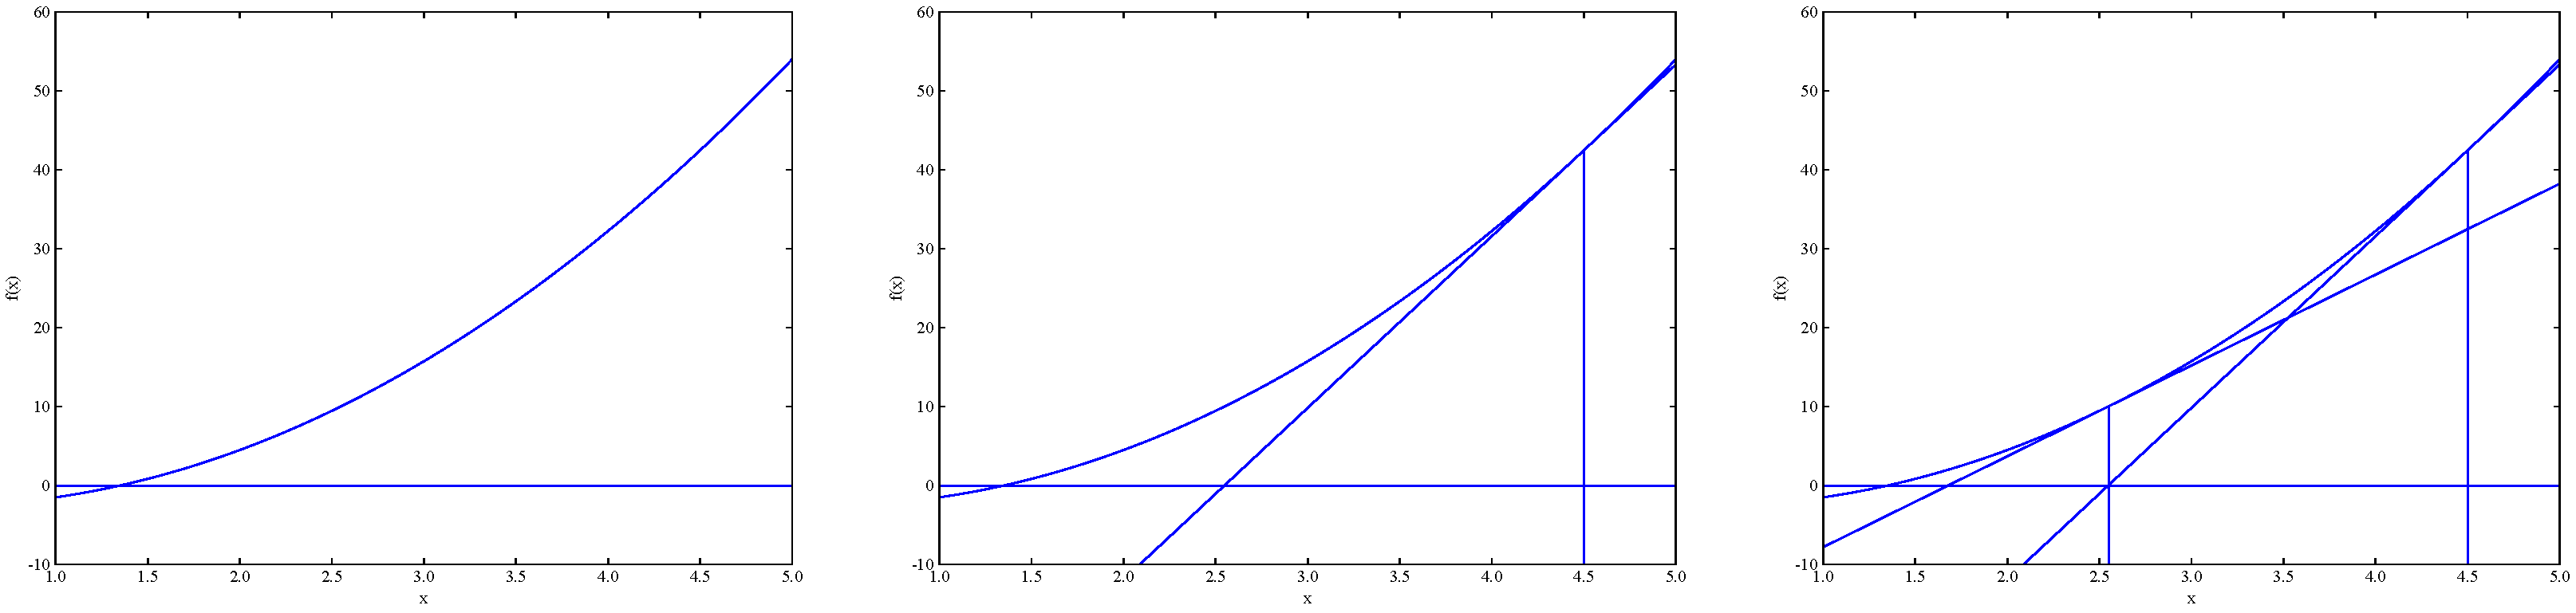
\includegraphics[width=0.93\linewidth]{figs/newton_iteration.pdf}
\end{figure}

\setcounter{footnote}{0}
\renewcommand{\thefootnote}{\fnsymbol{footnote}}
在最左边的图中,可以看到函数 $f$ 与直线 $y=0$。尝试找到一个 $\theta$ 使得 $f(\theta)=0$;实现这一点的 $\theta$ 值大约是 1.3。假设初始化的算法的 $\theta$ 值为 4.5。然后牛顿法拟合一条在 $\theta=4.5$ 处与 $f$ 相切的直线,并求解该直线等于 0 的点(中间图)。这给出了 $\theta$ 的下一个猜测值,大约是 2.6。最右边的图显示了再进行一次迭代的结果,更新后的 $\theta$ 大约是 1.6。再经过几次迭代后,将迅速接近 $\theta = 1.3$\footnote{译者注:由于不知道原书所用函数的解析形式,这里译者画的图与原图稍有偏差,$\theta$的猜测值也稍有变化。}。
\setcounter{footnote}{1}
\renewcommand{\thefootnote}{\arabic{footnote}}

牛顿法提供了一种求解 $f(\theta)=0$ 的方法。如果希望最大化某个函数 $\ell$ 呢? $\ell$ 的最大值对应于其一阶导数 $\ell'(\theta)$ 为零的点。因此,令 $f(\theta) = \ell'(\theta)$,可以使用相同的算法来最大化 $\ell$,并得到更新规则:
\[
    \theta := \theta - \frac{\ell'(\theta)}{\ell''(\theta)}.
\]
(思考题:如果希望使用牛顿法来最小化而不是最大化一个函数,这会如何改变?)

最后,在逻辑回归中,$\theta$ 是向量,因此需要将牛顿法推广到此情况。牛顿法在此多维设置中的推广(也称为牛顿-拉普森法)由下式给出
\[
    \theta := \theta - H^{-1} \nabla_\theta \ell(\theta).
\]
这里,$\nabla_\theta \ell(\theta)$ 是 $\ell(\theta)$ 对 $\theta_i$ 的偏导数向量,而 $H$ 是一个 $d \times d$ 矩阵(实际上,如果包含截距项,则是 $(d+1) \times (d+1)$ 矩阵),称为\textbf{Hessian} 矩阵,其元素由下式给出
\[
    H_{ij} = \frac{\partial^2 \ell(\theta)}{\partial \theta_i \partial \theta_j}.
\]
牛顿法通常比(批量)梯度下降收敛更快,并且需要更少的迭代次数即可非常接近最小值。然而,牛顿法迭代一次比梯度下降迭代一次更昂贵,因为它需要找到一个 $d \times d$ 的 Hessian 矩阵并求逆;但只要 $d$ 不太大,通常总体上会快得多。当牛顿法应用于最大化逻辑回归对数似然函数 $\ell(\theta)$ 时,所得方法也称为 \textbf{Fisher scoring}。

\chapter{广义线性模型}
到目前为止,我们已经讨论了一个回归示例和一个分类示例。在回归示例中,有 $y|x; \theta \sim \mathcal{N}(\mu, \sigma^2)$,在分类示例中,有 $y|x; \theta \sim \text{Bernoulli}(\phi)$,其中 $\mu$ 和 $\phi$ 是 $x$ 和 $\theta$ 的函数。在本节中,将展示这两种方法都是更广泛的模型族——称为广义线性模型(GLMs)\footnote{本节材料受到 Michael I. Jordan 的 \textit{Learning in graphical models}(未出版的书稿)以及 McCullagh 和 Nelder 的 \textit{Generalized Linear Models (2nd ed.)} 的启发。}——的特例。我们还将展示广义线性模型族中的其他模型如何推导并应用于其他分类和回归问题。

\section{指数族}

为了逐步了解广义线性模型,首先定义指数族分布。如果一类分布可以写成以下形式,则称其为指数族:
\begin{equation}
    p(y; \eta) = b(y) \exp(\eta^T T(y) - a(\eta))
    \label{eq:exp_family}
\end{equation}
这里,$\eta$ 称为\textbf{自然参数 (natural parameter)}(也称为\textbf{典范参数 (canonical parameter)});$T(y)$ 是\textbf{充分统计量 (sufficient statistic)}(对于所考虑的分布,通常有 $T(y)=y$);而 $a(\eta)$ 是\textbf{对数配分函数 (log partition function)}。量 $e^{-a(\eta)}$ 实际上起着归一化常数的作用,确保分布 $p(y; \eta)$ 在 $y$ 上的和或积分等于 1。

固定的 $T$, $a$ 和 $b$ 定义了一个由 $\eta$ 参数化的\textit{族 (family)}(或分布集);随着 $\eta$ 的变化,将得到该族中的不同分布。

现在展示伯努利分布和高斯分布是指数族分布的示例。具有均值 $\phi$ 的伯努利分布,记为 $\text{Bernoulli}(\phi)$,指定了在 $y \in \{0, 1\}$ 上的分布,使得 $p(y=1; \phi) = \phi$;$p(y=0; \phi) = 1-\phi$。随着 $\phi$ 的变化,可以得到具有不同均值的伯努利分布。现在我们推导改变 $\phi$ 得到的这些伯努利分布属于指数族;也就是说,存在一种 $T, a, b$ 的选择,使得公式 \eqref{eq:exp_family} 恰好成为伯努利分布。

将伯努利分布写为:
\[
\begin{aligned}
    p(y; \phi) &= \phi^y (1-\phi)^{1-y} \\
    &= \exp\left(y \log \phi + (1-y) \log(1-\phi)\right) \\
    &= \exp\left(\left(\log\left(\frac{\phi}{1-\phi}\right)\right)y + \log(1-\phi)\right).
\end{aligned}
\]
因此,自然参数由 $\eta = \log(\phi/(1-\phi))$ 给出。有趣的是,如果通过求解 $\phi$ 关于 $\eta$ 的表达式来反转这个定义,得到 $\phi = 1/(1+e^{-\eta})$。这是熟悉的 sigmoid 函数!在将逻辑回归推导为广义线性模型时,这将再次出现。为了完成伯努利分布作为指数族分布的形式化,还需要以下各项:
\[
\begin{aligned}
    T(y) &= y \\
    a(\eta) &= -\log(1-\phi) \\
    &= \log(1+e^\eta) \\
    b(y) &= 1
\end{aligned}
\]
这表明伯努利分布可以通过选择适当的 $T, a, b$ 从而写成公式 \eqref{eq:exp_family} 的形式。

接下来考虑高斯分布。回想一下,在线性回归推导中,$\sigma^2$ 的值对最终选择的 $\theta$ 和 $h_\theta(x)$ 没有影响。因此,可以在不改变任何内容的情况下选择任意的 $\sigma^2$ 值。为了简化下面的推导,令 $\sigma^2 = 1$。\footnote{如果将 $\sigma^2$ 作为一个变量,高斯分布也可以显示为指数族,其中 $\eta \in \mathbb{R}^2$ 现在是一个二维向量,它取决于 $\mu$ 和 $\sigma$。然而,出于广义线性模型的目的,$\sigma^2$ 参数也可以通过考虑指数族的一个更一般的定义来处理:$p(y; \eta, \tau) = b(a, \tau) \exp((\eta^T T(y) - a(\eta))/c(\tau))$。这里,$\tau$ 称为\textbf{散布参数 (dispersion parameter)},对于 高斯分布,$c(\tau) = \sigma^2$;但考虑到上面的简化,这里不需要更一般的定义。}有:
\[
\begin{aligned}
    p(y; \mu) &= \frac{1}{\sqrt{2\pi}} \exp\left(-\frac{1}{2}(y-\mu)^2\right) \\
    &= \frac{1}{\sqrt{2\pi}} \exp\left(-\frac{1}{2}y^2 + \mu y - \frac{1}{2}\mu^2\right) \\
    &= \frac{1}{\sqrt{2\pi}} \exp\left(-\frac{1}{2}y^2\right) \cdot \exp\left(\mu y - \frac{1}{2}\mu^2\right).
\end{aligned}
\]
因此, 高斯分布属于指数族,其中
\[
\begin{aligned}
    \eta &= \mu \\
    T(y) &= y \\
    a(\eta) &= \mu^2/2 \\
    &= \eta^2/2 \\
    b(y) &= (1/\sqrt{2\pi})\exp(-y^2/2).
\end{aligned}
\]

还有许多其他分布也属于指数族:多项分布(稍后将看到)、泊松分布(用于建模计数数据;另请参阅问题集)、伽马分布和指数分布(用于建模连续非负随机变量,例如时间间隔)、Beta 分布和 Dirichlet 分布(用于概率分布)等等。在下一节中,将描述构建模型的一般“配方”,其中 $y$(给定 $x$ 和 $\theta$)来自于这些分布中的任何一个。


\section{构造广义线性模型}

假设希望构建一个模型来估计在给定小时内到达商店的顾客数量(或网站的页面浏览量 $y$),基于某些特征 $x$,例如商店促销、近期广告、天气、星期几等等。已知泊松分布通常能很好地模拟访客数量。知道了这一点,如何为问题构建模型?幸运的是,泊松分布是指数族分布,因此可以应用广义线性模型。在本节中,将描述一种构建用于解决此类问题的广义线性模型的方法。

更一般地,考虑一个分类或回归问题,希望预测某个随机变量 $y$ 作为 $x$ 的函数的值。为了推导针对此问题的广义线性模型,将对给定 $x$ 的 $y$ 的条件分布和模型做出以下三个假设:

\begin{enumerate}
    \item $y|x; \theta \sim \text{ExponentialFamily}(\eta)$。也就是说,给定 $x$ 和 $\theta$, $y$ 的分布遵循参数为 $\eta$ 的某个指数族分布;
    \item 给定 $x$,目标是预测 $T(y)$ 的期望值。在大多数示例中,$T(y)=y$,因此这意味着希望学习到的假设 $h$ 的输出预测 $h(x)$ 满足 $h(x) = E[y|x]$。(注意,这个假设在逻辑回归和线性回归中对于 $h_\theta(x)$ 的选择是满足的。例如,在逻辑回归中,$h_\theta(x) = p(y=1|x; \theta) = 0 \cdot p(y=0|x; \theta) + 1 \cdot p(y=1|x; \theta) = E[y|x; \theta]$.);
    \item 自然参数 $\eta$ 和输入 $x$ 线性相关:$\eta = \theta^T x$。(或者,如果 $\eta$ 是向量值,则 $\eta_i = \theta_i^T x$.)
\end{enumerate}

第三个假设可能看起来最不合理,最好将其视为设计广义线性模型的“设计选择”,而不是一个固有的假设。这三个假设/设计选择将允许推导出非常优雅的一类学习算法,即广义线性模型,它们具有许多理想的特性,例如易于学习。此外,由此产生的模型对于建模不同类型的 $y$ 分布非常有效;例如,很快将展示逻辑回归和普通最小二乘都可以作为广义线性模型推导出来。

\subsection{普通最小二乘}

为了展示普通最小二乘是广义线性模型族的一个特例,考虑目标变量 $y$(在广义线性模型术语中也称为\textbf{响应变量 (response variable)})是连续的情况,并将给定 $x$ 的 $y$ 的条件分布建模为高斯分布 $N(\mu, \sigma^2)$。(这里,$\mu$ 可能取决于 $x$.)因此,令上面的 $\text{ExponentialFamily}(\eta)$ 分布为 高斯分布。如前所述,在将高斯分布公式化为指数族分布时,有 $\mu = \eta$。因此,有
\[
\begin{aligned}
    h_\theta(x) &= E[y|x; \theta] \\
    &= \mu \\
    &= \eta \\
    &= \theta^T x.
\end{aligned}
\]
第一个等号来自于上面的假设 2;第二个等号来自于 $y|x; \theta \sim N(\mu, \sigma^2)$,因此其期望值由 $\mu$ 给出;第三个等号来自于假设 1(以及之前推导中表明在将高斯分布公式化为指数族分布时 $\mu = \eta$);最后一个等号来自于假设 3。

\subsection{逻辑回归}

现在考虑逻辑回归。这里感兴趣的是二分类问题,因此 $y \in \{0, 1\}$。鉴于 $y$ 是二值变量,选择伯努利分布族来建模给定 $x$ 的 $y$ 的条件分布是很自然的。在将伯努利分布公式化为指数族分布时,有 $\phi = 1/(1 + e^{-\eta})$。此外,注意如果 $y|x; \theta \sim \text{Bernoulli}(\phi)$,则 $E[y|x; \theta] = \phi$。因此,按照与普通最小二乘类似的推导,得到:
\[
\begin{aligned}
    h_\theta(x) &= E[y|x; \theta] \\
    &= \phi \\
    &= 1/(1 + e^{-\eta}) \\
    &= 1/(1 + e^{-\theta^T x})
\end{aligned}
\]
因此,这给出了形式为 $h_\theta(x) = 1/(1 + e^{-\theta^T x})$ 的假设函数。如果之前曾想知道如何得到逻辑函数 $1/(1 + e^{-z})$ 的形式,这就是一个答案:一旦假设给定 $x$ 的 $y$ 服从伯努利分布,它就作为广义线性模型和指数族分布定义的必然结果出现了。

这里引入一些额外的术语,将自然参数映射到分布均值的函数 $g$($g(\eta) = E[T(y); \eta]$),称为\textbf{典范响应函数 (canonical response1 function)}。其逆函数 $g^{-1}$ 称为\textbf{典范连接函数 (canonical link function)}。因此,高斯族分布的典范响应函数就是恒等函数;伯努利分布的典范响应函数是逻辑函数\footnote{许多文献使用 $g$ 表示连接函数,$g^{-1}$ 表示响应函数;但这里使用的符号继承自早期的机器学习文献,将与课程其余部分使用的符号更一致。}。

\chapter{生成式学习算法}

到目前为止,我们讨论的主要是学习这样的一类算法,这些算法建模给定 $x$ 的情况下 $y$ 的条件分布 $p(y|x; \theta)$。例如,逻辑回归将 $p(y|x; \theta)$ 建模为 $h_\theta(x) = g(\theta^T x)$,其中 $g$ 是 sigmoid 函数。在本章中,将讨论一种不同类型的学习算法。

考虑一个分类问题,其中希望根据动物的一些特征来区分大象 ($y=1$) 和狗 ($y=0$)。给定一个训练集,像逻辑回归或感知机算法(本质上)试图找到一条直线——也就是一个决策边界——来分隔大象和狗。然后,为了将新动物分类为大象或狗,检查其落在决策边界的哪一侧,并据此做出预测。

这里介绍一种不同的方法。首先,观察大象,可以建立一个关于大象外观的模型。然后,观察狗,可以建立一个关于狗外观的独立模型。最后,为了对新动物进行分类,可以将新动物与大象模型进行匹配,并将其与狗模型进行匹配,以查看新动物是否更像在训练集中看到的大象或狗。

试图直接学习 $p(y|x)$ 的算法(如逻辑回归),或试图直接学习从输入空间 $\mathcal{X}$ 到标签 $\{0, 1\}$ 的映射的算法(如感知机算法)称为\textbf{判别式 (discriminative)} 学习算法。这里,将讨论那些试图建模 $p(x|y)$(和 $p(y)$)的算法。这些算法称为\textbf{生成式 (generative)} 学习算法。例如,如果 $y$ 表示一个样本是狗 ($0$) 还是大象 ($1$),则 $p(x|y=0)$ 建模狗的特征分布,$p(x|y=1)$ 建模大象的特征分布。

在建模 $p(y)$(称为\textbf{类先验 (class priors)})和 $p(x|y)$ 之后,算法可以利用贝叶斯定理推导出给定 $x$ 时 $y$ 的后验分布:
\[
    p(y|x) = \frac{p(x|y)p(y)}{p(x)}.
\]
这里,分母由 $p(x) = p(x|y=1)p(y=1) + p(x|y=0)p(y=0)$ 给出(根据概率的标准性质,可以验证这一点),因此也可以用学到的 $p(x|y)$ 和 $p(y)$ 来表示。实际上,如果计算 $p(y|x)$ 是为了进行预测,那么并不需要计算分母,因为
\[
\begin{aligned}
    \arg \max_y p(y|x) &= \arg \max_y \frac{p(x|y)p(y)}{p(x)} \\
    &= \arg \max_y p(x|y)p(y).
\end{aligned}
\]

\section{高斯判别分析}

将要介绍的第一个生成式学习算法是高斯判别分析 (GDA)。在这个模型中,假设 $p(x|y)$ 服从多元正态分布。在介绍 GDA 模型本身之前,先简要讨论一下多元正态分布的性质。

\subsection{多元正态分布}

$d$ 维的多元正态分布,也称为多元高斯分布,由\textbf{均值向量 (mean vector)} $\mu \in \mathbb{R}^d$ 和\textbf{协方差矩阵 (covariance matrix)} $\Sigma \in \mathbb{R}^{d \times d}$ 参数化,其中 $\Sigma \ge 0$ 是对称正半定矩阵。其密度函数写为 $\mathcal{N}(\mu, \Sigma)$,形式如下:
\[
    p(x; \mu, \Sigma) = \frac{1}{(2\pi)^{d/2}|\Sigma|^{1/2}} \exp\left(-\frac{1}{2}(x-\mu)^T \Sigma^{-1}(x-\mu)\right).
\]
在上面的方程中,$|\Sigma|$ 表示矩阵 $\Sigma$ 的行列式。
对于服从 $\mathcal{N}(\mu, \Sigma)$ 分布的随机变量 $X$,其均值(毫不意外地)由 $\mu$ 给出:
\[
    \mathrm{E}[X] = \int_x x p(x; \mu, \Sigma) dx = \mu
\]
向量值随机变量 $Z$ 的\textbf{协方差}定义为 $\text{Cov}(Z) = \mathrm{E}[(Z - \mathrm{E}[Z])(Z - \mathrm{E}[Z])^T]$。这推广了实值随机变量的方差概念。协方差也可以定义为 $\text{Cov}(Z) = \mathrm{E}[ZZ^T] - (\mathrm{E}[Z])(\mathrm{E}[Z])^T$。(可以自行证明这两个定义是等价的。)如果 $X \sim \mathcal{N}(\mu, \Sigma)$,则
\[
    \mathrm{Cov}(X) = \Sigma.
\]

以下是一些高斯分布密度函数的示例:

\begin{figure}[H]
    \centering
    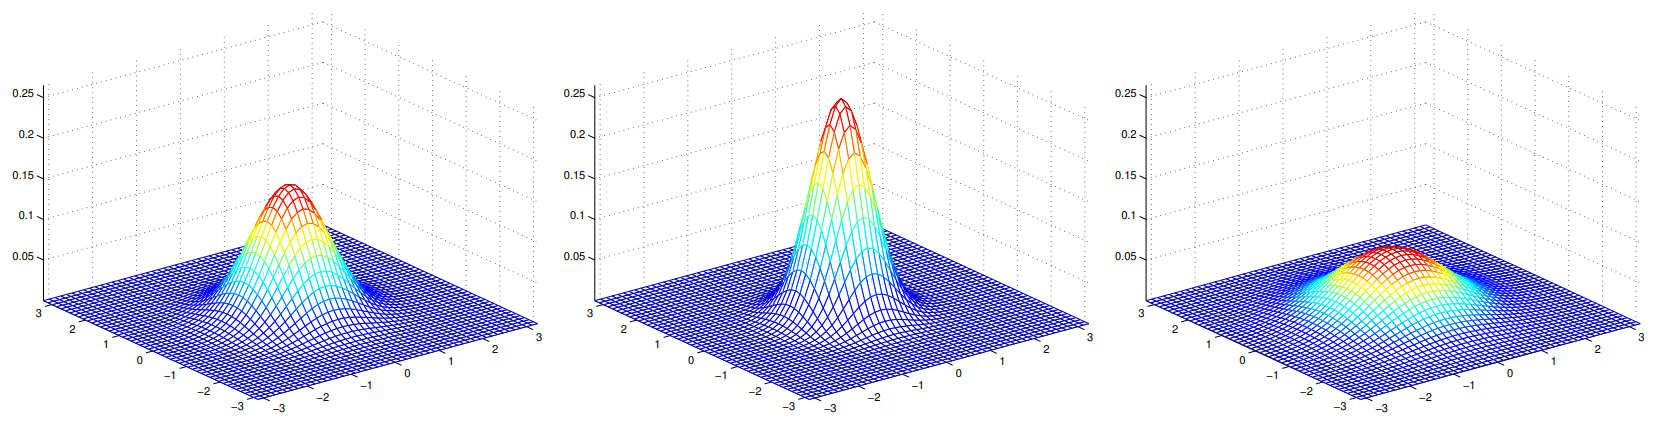
\includegraphics[width=1.0\linewidth]{figs/gaussian_density1.png}
\end{figure}

最左边的图显示的是均值为零(即 $2 \times 1$ 零向量)、协方差矩阵为 $\Sigma = I$(即 $2 \times 2$ 单位矩阵)的高斯分布。均值为零、协方差为单位矩阵的高斯分布也称为\textbf{标准正态分布}。中间的图显示的是均值为零、$\Sigma = 0.6I$ 的高斯分布的密度;最右边的图显示的是 $\Sigma = 2I$ 的高斯分布的密度。可以看到,随着 $\Sigma$ 变大,高斯分布变得更加“分散”,而随着 $\Sigma$ 变小,分布变得更加“紧凑”。

接下来看一些更多的例子。

\begin{figure}[H]
    \centering
    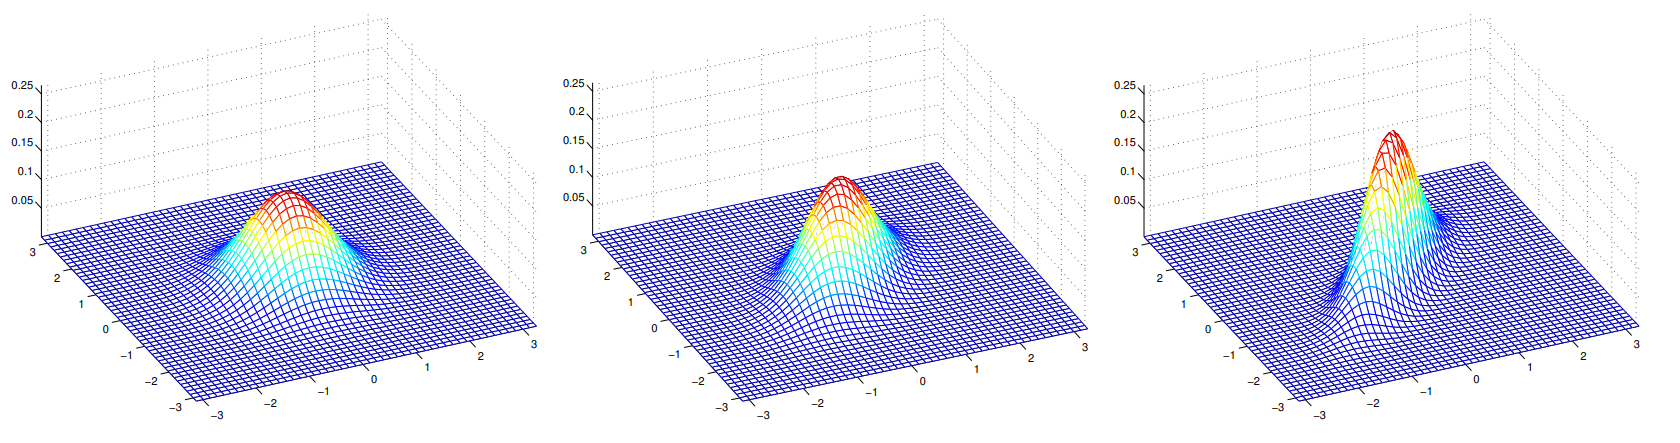
\includegraphics[width=1.0\linewidth]{figs/gaussian_density2.png}
\end{figure}

上面的图显示了均值为 0、协方差矩阵分别为
\[
    \Sigma = \begin{bmatrix} &1& &0& \\ &0& &1& \end{bmatrix}; \Sigma = \begin{bmatrix} &1& &0.5& \\ &0.5& &1& \end{bmatrix}; \Sigma = \begin{bmatrix} &1& &0.8& \\ &0.8& &1& \end{bmatrix}.
\]
最左边的图显示的是熟悉的标准正态分布,并且可以看到,随着 $\Sigma$ 中非对角线元素的增加,密度函数变得更加“压缩”到 $45^\circ$ 线(由 $x_1 = x_2$ 给出)。当观察这三个密度函数的等高线时,可以更清楚地看到这一点:

\begin{figure}[H]
    \centering
    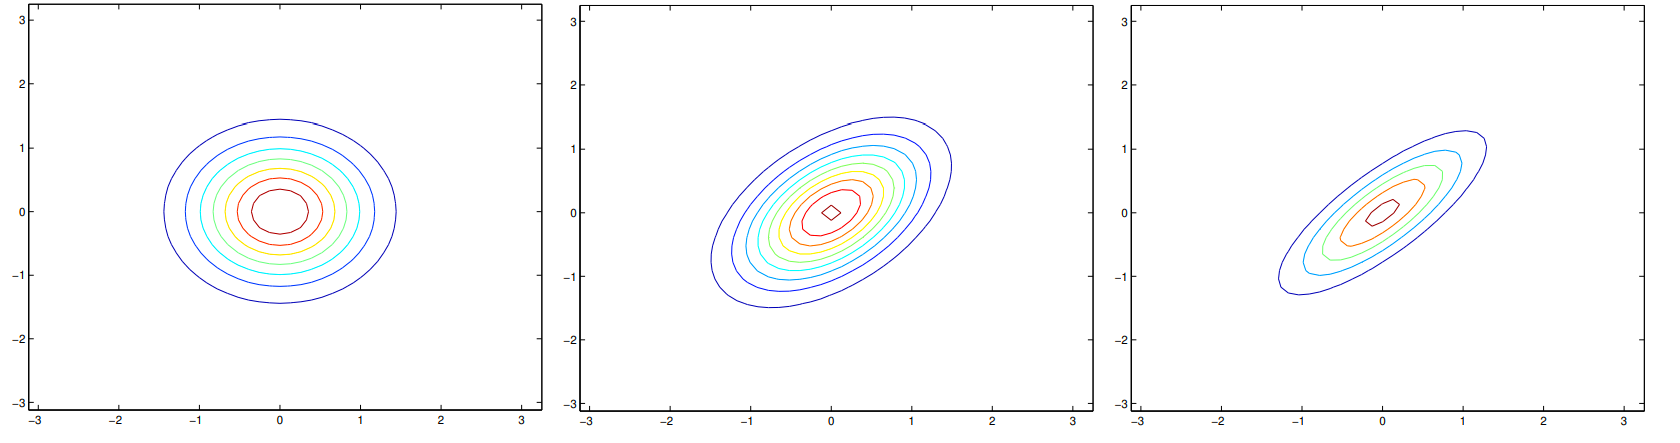
\includegraphics[width=1.0\linewidth]{figs/gaussian_contour1.png}
\end{figure}

下面是另外一组由不同的 $\Sigma$ 生成的例子:

\begin{figure}[H]
    \centering
    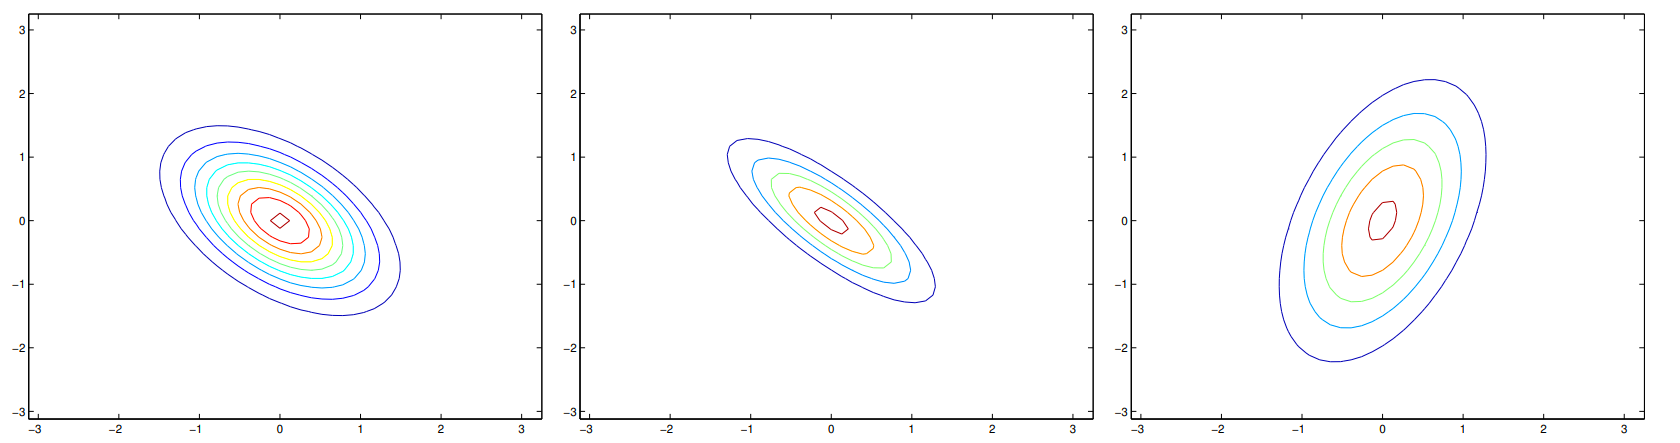
\includegraphics[width=1.0\linewidth]{figs/gaussian_contour2.png}
\end{figure}

上面的图分别使用了
\[
    \Sigma = \begin{bmatrix} &1& &-0.5& \\ &-0.5& &1& \end{bmatrix}; \Sigma = \begin{bmatrix} &1& &-0.8& \\ &-0.8& &1& \end{bmatrix}; \Sigma = \begin{bmatrix} &3& &0.8& \\ &0.8& &1& \end{bmatrix}.
\]
从最左边和中间的图可以看到,通过减小协方差矩阵的非对角线元素,密度函数再次变得“压缩”,但方向相反。最后值得一提的是,当改变参数时,等高线通常会形成椭圆(最右边的图显示了一个例子)。

作为最后一组例子,通过固定 $\Sigma = I$,并改变 $\mu$,也可以移动密度函数的均值。

\begin{figure}[H]
    \centering
    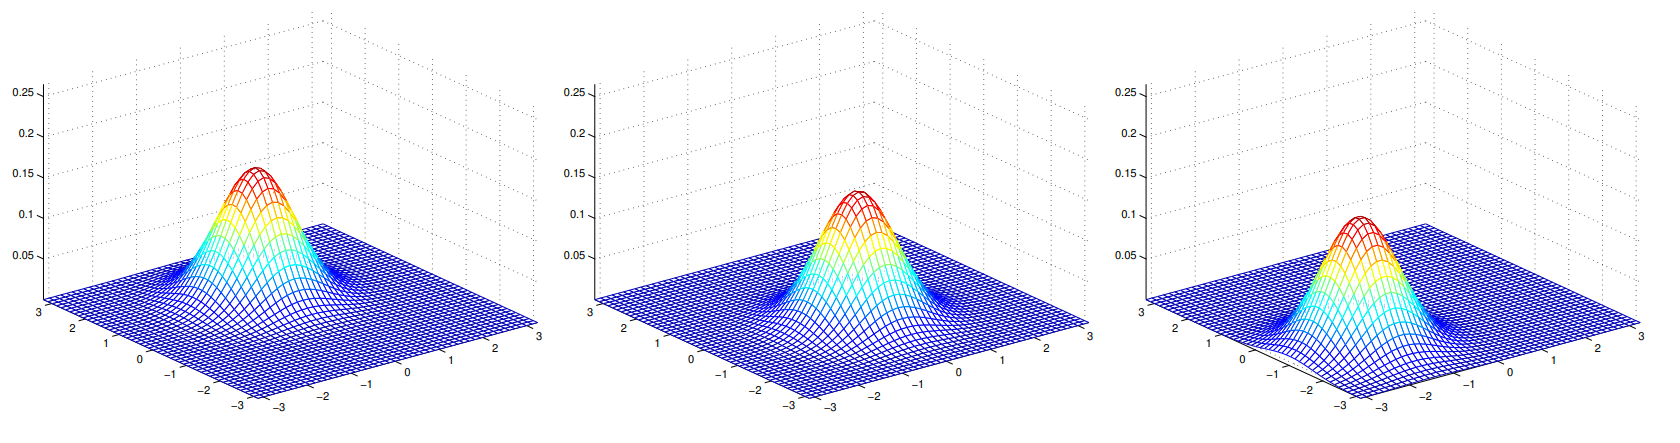
\includegraphics[width=1.0\linewidth]{figs/gaussian_density3.png}
\end{figure}

上面的图是使用 $\Sigma = I$ 生成的,并且 $\mu$ 分别为
\[
    \mu = \begin{bmatrix} &1& \\ &0& \end{bmatrix}; \mu = \begin{bmatrix} &-0.5& \\ &0& \end{bmatrix}; \mu = \begin{bmatrix} &-1& \\ &-1.5& \end{bmatrix}.
\]

\subsection{高斯判别分析模型}

当遇到输入特征 $x$ 是连续随机变量的分类问题时,可以使用高斯判别分析模型,该模型利用多元正态分布对 $p(x|y)$ 进行建模。模型如下:
\[
\begin{aligned}
    y &\sim \text{Bernoulli}(\phi) \\
    x|y=0 &\sim \mathcal{N}(\mu_0, \Sigma) \\
    x|y=1 &\sim \mathcal{N}(\mu_1, \Sigma)
\end{aligned}
\]
写出分布形式为:
\[
\begin{aligned}
    p(y) &= \phi^y (1-\phi)^{1-y} \\
    p(x|y=0) &= \frac{1}{(2\pi)^{d/2}|\Sigma|^{1/2}} \exp\left(-\frac{1}{2}(x-\mu_0)^T \Sigma^{-1} (x-\mu_0)\right) \\
    p(x|y=1) &= \frac{1}{(2\pi)^{d/2}|\Sigma|^{1/2}} \exp\left(-\frac{1}{2}(x-\mu_1)^T \Sigma^{-1} (x-\mu_1)\right)
\end{aligned}
\]
模型中的参数为 $\phi, \Sigma, \mu_0$ 和 $\mu_1$。(注意,尽管有两个不同的均值向量 $\mu_0$ 和 $\mu_1$,但该模型通常只使用一个协方差矩阵 $\Sigma$。) 数据的对数似然函数如下:
\[
\begin{aligned}
    \ell(\phi, \mu_0, \mu_1, \Sigma) &= \log \prod_{i=1}^n p(x^{(i)}, y^{(i)}; \phi, \mu_0, \mu_1, \Sigma) \\
    &= \log \prod_{i=1}^n p(x^{(i)}|y^{(i)}; \mu_0, \mu_1, \Sigma) p(y^{(i)}; \phi).
\end{aligned}
\]

通过最大化 $\ell$ 对参数进行估计,可以得到参数的最大似然估计(参见习题集 1):
\[
\begin{aligned}
    \phi &= \frac{1}{n} \sum_{i=1}^n 1\{y^{(i)} = 1\} \\
    \mu_0 &= \frac{\sum_{i=1}^n 1\{y^{(i)} = 0\}x^{(i)}}{\sum_{i=1}^n 1\{y^{(i)} = 0\}} \\
    \mu_1 &= \frac{\sum_{i=1}^n 1\{y^{(i)} = 1\}x^{(i)}}{\sum_{i=1}^n 1\{y^{(i)} = 1\}} \\
    \Sigma &= \frac{1}{n} \sum_{i=1}^n (x^{(i)} - \mu_{y^{(i)}})(x^{(i)} - \mu_{y^{(i)}})^T.
\end{aligned}
\]

从直观上看,算法的操作可以表示如下:

\begin{figure}[H]
    \centering
    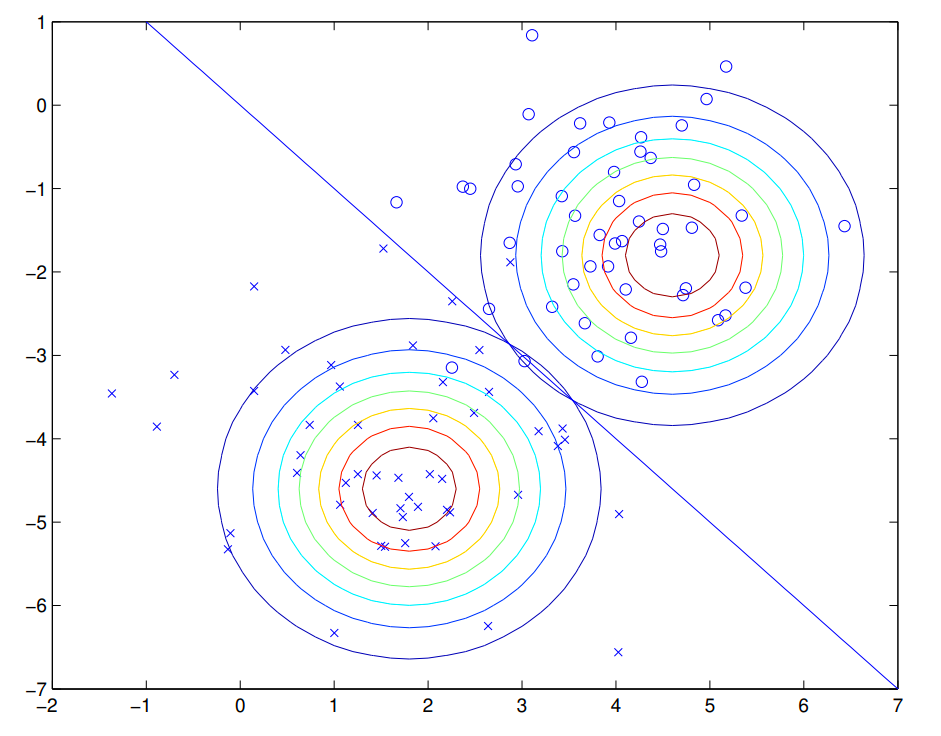
\includegraphics[width=0.5\linewidth]{figs/gda.png}
\end{figure}

图中展示了训练集以及拟合到两个类别数据的两个高斯分布的等高线。注意到由于共享协方差矩阵 $\Sigma$,这两个高斯分布的等高线形状和方向相同,但它们的均值 $\mu_0$ 和 $\mu_1$ 不同。图中还展示了 $p(y=1|x)=0.5$ 的决策边界直线。在边界的一侧,预测 $y=1$ 是最可能的结果,而在另一侧,则更多地预测 $y=0$。

\subsection{讨论:GDA 与逻辑回归}

GDA 模型与逻辑回归有着有趣的关系。如果将 $p(y=1|x; \phi, \mu_0, \mu_1, \Sigma)$ 视为 $x$ 的函数,会发现它可以表示为以下形式:
\[
    p(y=1|x; \phi, \mu_0, \mu_1, \Sigma) = \frac{1}{1+\exp(-\theta^T x)},
\]
其中 $\theta$ 是 $\phi, \mu_0, \mu_1, \Sigma$ 的适当函数。\footnote{这里采用了重新定义右侧 $x^{(i)}$ 为 $(d+1)$ 维向量的约定,即添加额外的坐标 $x_0^{(i)} = 1$;参见习题集 1。} 这正是逻辑回归(一种判别式算法)用来建模 $p(y=1|x)$ 的形式。

何时应该优先选择其中一个模型,何时又该选择另一个?GDA 和逻辑回归在同一数据集上训练时,通常会给出不同的决策边界,如何判断哪个会更好?

前文论述了,如果 $p(x|y)$ 是多元高斯分布(且共享 $\Sigma$),那么 $p(y|x)$ 必然是逻辑函数。反之则不成立,即 $p(y|x)$ 是逻辑函数并不意味着 $p(x|y)$ 是多元高斯分布。这表明 GDA 对数据做出了比逻辑回归更强的建模假设。事实证明,当这些建模假设正确时,GDA 会更好地拟合数据,并且是一个更好的模型。具体来说,当 $p(x|y)$ 确实是高斯分布(且共享 $\Sigma$)时,GDA 具有\textbf{渐近效率 (asymptotically efficient)}。非正式地讲,这意味着在训练集非常大($n$ 很大)的极限情况下,没有哪个算法能比 GDA 更好(例如,在估计 $p(y|x)$ 的准确性方面)。特别地,在这种情况下,可以证明 GDA 是比逻辑回归更好的算法;更一般地,即使训练集较小,通常也期望 GDA 表现更好。

相比之下,通过做出显著较弱的假设,逻辑回归也更\textit{鲁棒 (Robust)},对不正确的建模假设更不敏感。有许多不同的假设集合可以导致 $p(y|x)$ 呈现逻辑函数的形式。例如,如果 $x|y=0 \sim \text{Poisson}(\lambda_0)$ 且 $x|y=1 \sim \text{Poisson}(\lambda_1)$,那么 $p(y|x)$ 将是逻辑函数。逻辑回归在这种泊松分布数据上也能很好地工作。但是,如果对非高斯数据使用 GDA 并拟合高斯分布,那么结果将不太可预测,并且 GDA 可能表现不佳。

总结来说:GDA 做出了更强的建模假设,并且在建模假设正确或至少近似正确时,数据效率更高(即,需要较少的训练数据来“很好地”学习)。逻辑回归做出了较弱的假设,并且对建模假设的错误更鲁棒。具体来说,当数据确实是非高斯分布时,在大数据集的极限情况下,逻辑回归几乎总是比 GDA 表现更好。因此,在实践中,逻辑回归比 GDA 使用更频繁。(关于判别式模型与生成式模型的某些相关考虑也适用于接下来讨论的朴素贝叶斯算法,但朴素贝叶斯算法仍然被认为是一个非常好的,并且当然也是一个非常流行的分类算法。)

\section{朴素贝叶斯(选读)}

在 GDA 中,特征向量 $x$ 是连续的实值向量。接下来讨论一种不同的学习算法,其中 $x_j$ 是离散值。

以构建电子邮件垃圾邮件过滤器为例,考虑使用机器学习。希望根据消息是否为未经请求的商业(垃圾邮件)或非垃圾邮件来对其进行分类。学习完成后,可以使邮件阅读器自动过滤掉垃圾邮件,并将其放入单独的文件夹中。对电子邮件进行分类是更广泛的问题集合(称为\textbf{文本分类 (text classification)})的一个示例。

假设有一个训练集(一组标记为垃圾邮件或非垃圾邮件的电子邮件)。首先通过指定用于表示电子邮件的特征 $x_j$ 来构建垃圾邮件过滤器。

将通过一个特征向量来表示一封电子邮件,该向量的长度等于字典中的单词数量。具体来说,如果一封电子邮件包含字典中的第 $j$ 个单词,则设置 $x_j=1$;否则,设置 $x_j=0$。例如,以下向量:


\[
x = 
\begin{bmatrix}
    &1& \\
    &0& \\
    &0& \\
    &\vdots& \\
    &1& \\
    &\vdots& \\
    &0&
\end{bmatrix}
\quad % 或者 \qquad 调整间距
\begin{array}{l}
    \text{a} \\
    \text{aardvark} \\
    \text{aardwolf} \\
    \vdots \\
    \text{buy} \\
    \vdots \\
    \text{zygmurgy}
\end{array}
\]
表示一封包含单词“a”和“buy”但不包含“aardvark”、“aardwolf”或“zygmurgy”的电子邮件。\footnote{实际上,在实践中会查看训练集并仅将至少出现一次的单词编码到特征向量中,而不是查看所有英文单词的列表。除了减少建模的单词数量,从而降低计算和空间需求外,这还有一个优点,即允许对可能出现在电子邮件中(例如“cs229”)但在字典中找不到的许多单词进行建模/包含作为特征。有时(在作业中)还会排除非常高频的单词(例如“the”、“of”和“and”);这些高频的“无内容”词被称为\textbf{停用词 (stop words)},因为它们在许多文档中都会出现,并且很少能表明电子邮件是垃圾邮件还是非垃圾邮件。} 用于编码特征向量的单词集合称为\textbf{词汇表 (vocabulary)},因此 $x$ 的维度等于词汇表的大小。

在选择了特征向量之后,现在希望构建一个生成模型。因此,需要对 $p(x|y)$ 进行建模。但是,如果词汇表有 50000 个单词,那么 $x \in \{0, 1\}^{50000}$($x$ 是一个由 0 和 1 组成的 50000 维向量),如果对 $x$ 使用 2$^{50000}$ 种可能结果的多项分布进行显式建模,最终会得到一个 $(2^{50000}-1)$ 维参数向量。参数数量显然太多了。

因此,为了对 $p(x|y)$ 进行建模,将做出一个非常强的假设。假设给定 $y$ 时,$x_i$ 是条件独立的。这个假设称为\textbf{朴素贝叶斯假设 (Naive Bayes (NB) assumption)},由此产生的算法称为\textbf{朴素贝叶斯分类器 (Naive Bayes classifier)}。例如,如果 $y=1$ 表示垃圾邮件,“buy”是第 2087 个单词,“price”是第 39831 个单词;那么假设如果知道 $y=1$(这封特定的电子邮件是垃圾邮件),那么关于 $x_{2087}$ 的知识(消息中是否出现“buy”)对关于 $x_{39831}$ 的值(是否出现“price”)的信念没有影响。更正式地讲,这可以写成 $p(x_{2087}|y) = p(x_{2087}|y, x_{39831})$。(注意,这与 $x_{2087}$ 和 $x_{39831}$ 是独立的说法不同,独立的说法会写成 $p(x_{2087}) = p(x_{2087}|x_{39831})$;相反,这里只假设给定 $y$ 时,$x_{2087}$ 和 $x_{39831}$ 是条件独立的。)

现在有:
\[
    \begin{aligned}
        p(x_1, \dots, x_{50000}|y) &= p(x_1|y)p(x_2|y, x_1)p(x_3|y, x_1, x_2) \cdots p(x_{50000}|y, x_1, \dots, x_{49999}) \\ 
        &= p(x_1|y)p(x_2|y)p(x_3|y) \cdots p(x_{50000}|y) \\ 
        &= \prod_{j=1}^d p(x_j|y) 
    \end{aligned}
\]
第一个等号仅遵循概率的通常性质,第二个等号使用了朴素贝叶斯假设。注意,尽管朴素贝叶斯假设是一个非常强的假设,但由此产生的算法在许多问题上效果很好。

模型由 $\phi_{j|y=1} = p(x_j=1|y=1)$、$\phi_{j|y=0} = p(x_j=1|y=0)$ 和 $\phi_y = p(y=1)$ 参数化。像往常一样,给定训练集 $\{(x^{(i)}, y^{(i)}); i=1, \dots, n\}$,可以写出数据的联合似然:
\[
    \mathcal{L}(\phi_y, \phi_{j|y=0}, \phi_{j|y=1}) = \prod_{i=1}^n p(x^{(i)}, y^{(i)}).
\]
关于 $\phi_y$、$\phi_{j|y=0}$ 和 $\phi_{j|y=1}$ 最大化此式,得到最大似然估计:
\[
    \begin{aligned}
        \phi_{j|y=1} &= \frac{\sum_{i=1}^n {1}\{x_j^{(i)} = 1 \wedge y^{(i)} = 1\}}{\sum_{i=1}^n {1}\{y^{(i)} = 1\}} \\ 
        \phi_{j|y=0} &= \frac{\sum_{i=1}^n {1}\{x_j^{(i)} = 1 \wedge y^{(i)} = 0\}}{\sum_{i=1}^n {1}\{y^{(i)} = 0\}} \\ 
        \phi_y &= \frac{\sum_{i=1}^n {1}\{y^{(i)} = 1\}}{n} 
    \end{aligned}
\]
在上面的公式中,“$\wedge$”符号表示“逻辑且”。参数具有非常自然的解释。例如,$\phi_{j|y=1}$ 是单词 $j$ 出现在垃圾邮件 ($y=1$) 中的比例。

在拟合了所有这些参数之后,为了对具有特征 $x$ 的新示例进行预测,只需计算:
\[
\begin{aligned}
    p(y=1|x) &= \frac{p(x|y=1)p(y=1)}{p(x)} \\
    &= \frac{\left(\prod_{j=1}^d p(x_j|y=1)\right) p(y=1)}{\left(\prod_{j=1}^d p(x_j|y=1)\right) p(y=1) + \left(\prod_{j=1}^d p(x_j|y=0)\right) p(y=0)},
\end{aligned}
\]
并选择后验概率较高的类别。

最后,注意,虽然主要针对特征 $x_j$ 是二值的问题开发了朴素贝叶斯算法,但可以很直接地将其推广到 $x_j$ 可以取 $\{1, 2, \dots, k_j\}$ 中的值,只需将 $p(x_j|y)$ 建模为多项分布而不是伯努利分布。实际上,即使某些原始输入属性(例如,之前示例中的房屋居住面积)是连续值,通常也会将其\textbf{离散化 (discretize)}——即将其转换为一小组离散值,然后应用朴素贝叶斯。例如,如果使用某个特征 $x_j$ 来表示居住面积,可以将连续值离散化如下:

\begin{table}[H]
    \centering
    \begin{tabular}{c|c|c|c|c|c}
        居住面积 (平方英尺) & < 400 & 400-800 & 800-1200 & 1200-1600 & > 1600 \\
        \hline
        $x_i$ & 1 & 2 & 3 & 4 & 5 
    \end{tabular}
\end{table}

因此,对于居住面积为 890 平方英尺的房屋,可以将相应的特征 $x_j$ 的值设置为 3。然后可以应用朴素贝叶斯算法,并如前所述,使用多项分布对 $p(x_j|y)$ 进行建模。当原始的连续值属性无法通过多元正态分布很好地建模时,离散化特征并使用朴素贝叶斯(而不是 GDA)通常会产生更好的分类器。

\subsection{拉普拉斯平滑}

如前所述,朴素贝叶斯算法在许多问题上效果相当不错,但有一个简单的修改可以使其效果更好,尤其是在文本分类方面。简要讨论一下该算法当前形式存在的问题,然后讨论如何解决它。

考虑垃圾邮件/电子邮件分类,假设于 20xx 年,在您 CS229 结课并出色地完成了项目后,您决定在 20xx 年 5 月左右提交您的工作以在 NeurIPS 会议上发表。\footnote{NeurIPS 是顶级机器学习会议之一。提交论文的截止日期通常在五月至六月。} 因为会在电子邮件中讨论该会议,所以您也开始收到包含“neurips”一词的消息。但这是您的第一篇 NeurIPS 论文,在此之前,您从未见过包含“neurips”一词的电子邮件;特别是在垃圾邮件/非垃圾邮件训练集中,“neurips”从未出现过。假设“neurips”是字典中的第 35000 个单词,您的朴素贝叶斯垃圾邮件过滤器会选择其最大似然估计参数 $\phi_{35000|y}$ 为:

\begin{align*} 
\phi_{35000|y=1} &= \frac{\sum_{i=1}^n {1}\{x_{35000}^{(i)} = 1 \wedge y^{(i)} = 1\}}{\sum_{i=1}^n {1}\{y^{(i)} = 1\}} = 0 \\ \phi_{35000|y=0} &= \frac{\sum_{i=1}^n {1}\{x_{35000}^{(i)} = 1 \wedge y^{(i)} = 0\}}{\sum_{i=1}^n {1}\{y^{(i)} = 0\}} = 0 
\end{align*}
也就是说,由于它从未在垃圾邮件或非垃圾邮件训练示例中见过“neurips”,它认为在任何类型的电子邮件中看到它的概率为零。因此,当尝试判断这些包含“neurips”的消息是否是垃圾邮件时,它会计算类别后验概率,并得到
\[
    p(y=1|x) = \frac{\prod_{j=1}^d p(x_j|y=1) p(y=1)}{\prod_{j=1}^d p(x_j|y=1) p(y=1) + \prod_{j=1}^d p(x_j|y=0) p(y=0)} = \frac{0}{0}.
\]
这是因为 $\prod_{j=1}^d p(x_j|y)$ 的每一项都包含一个 $p(x_{35000}|y) = 0$ 的项,该项与乘积相乘。因此,算法得到 0/0,无法做出预测。

更广泛地说,仅仅因为在有限的训练集中没有看到某个事件,就将其概率估计为零,这在统计上是一个糟糕的主意。考虑估计一个多项随机变量 $z$ 取值为 $\{1, \dots, k\}$ 的问题。可以用 $\phi_j = p(z=j)$ 参数化多项分布。给定一组 $n$ 个独立观测值 $\{z^{(1)}, \dots, z^{(n)}\}$,最大似然估计由下式给出:
\[
    \phi_j = \frac{\sum_{i=1}^n {1}\{z^{(i)} = j\}}{n}.
\]
正如之前看到的,如果使用这些最大似然估计,那么一些 $\phi_j$ 可能会变为零,这是一个问题。为了避免这种情况,可以使用\textbf{拉普拉斯平滑 (Laplace smoothing)},它将上述估计替换为:
\[
    \phi_j = \frac{1 + \sum_{i=1}^n {1}\{z^{(i)} = j\}}{k + n}.
\]
在这里,在分子中加了 1,在分母中加了 $k$。注意,$\sum_{j=1}^k \phi_j = 1$ 仍然成立(自己验证一下!),这是一个理想的属性,因为 $\phi_j$ 是概率的估计,而概率之和必须为 1。此外,对于所有 $j$ 的值,$\phi_j \ne 0$,解决了概率估计为零的问题。在某些(可以说相当强的)条件下,可以证明拉普拉斯平滑实际上给出了 $\phi_j$ 的最优估计。

回到朴素贝叶斯分类器,使用拉普拉斯平滑,因此得到以下参数估计:
\begin{align*} \phi_{j|y=1} &= \frac{1 + \sum_{i=1}^n {1}\{x_j^{(i)} = 1 \wedge y^{(i)} = 1\}}{2 + \sum_{i=1}^n {1}\{y^{(i)} = 1\}} \\ \phi_{j|y=0} &= \frac{1 + \sum_{i=1}^n {1}\{x_j^{(i)} = 1 \wedge y^{(i)} = 0\}}{2 + \sum_{i=1}^n {1}\{y^{(i)} = 0\}} \end{align*}
(在实践中,是否对 $\phi_y$ 应用拉普拉斯平滑通常无关紧要,因为通常垃圾邮件和非垃圾邮件的比例都相当可观,所以 $\phi_y$ 将是 $p(y=1)$ 的合理估计,并且无论如何都会远离 0。)

\subsection{文本分类的事件模型}

为了结束关于生成学习算法的讨论,下面讨论一个专门用于文本分类的模型。虽然前面介绍的朴素贝叶斯在许多分类问题上效果很好,但对于文本分类,有一个相关的模型效果更好。

在文本分类的具体背景下,前面介绍的朴素贝叶斯使用了\textbf{伯努利事件模型 (Bernoulli event model)}(或有时称为\textbf{多元伯努利事件模型 (multi-variate Bernoulli event model)})。在该模型中,假设生成电子邮件的过程是:首先随机确定(根据类别先验 $p(y)$)发送者是垃圾邮件发送者还是非垃圾邮件发送者。然后,发送电子邮件的人遍历字典,独立地决定是否根据概率 $p(x_j=1|y) = \phi_{j|y}$ 在该电子邮件中包含每个单词 $j$。因此,消息的概率由 $p(y) \prod_{j=1}^d p(x_j|y)$ 给出。

这里有一个不同的模型,称为\textbf{多项事件模型 (Multinomial event model)}。为了描述该模型,将使用不同的表示法和特征集来表示电子邮件。令 $x_j$ 表示电子邮件中第 $j$ 个单词的标识。因此,$x_j$ 现在是一个整数,取值范围为 $\{1, \dots, |V|\}$,其中 $|V|$ 是词汇表(字典)的大小。包含 $d$ 个单词的电子邮件现在由一个长度为 $d$ 的向量 $(x_1, x_2, \dots, x_d)$ 表示;注意 $d$ 可以因不同的文档而异。例如,如果一封电子邮件以“A NeurIPS ...”开头,那么 $x_1=1$(“a”是字典中的第一个单词),$x_2=35000$(如果“neurips”是字典中的第 35000 个单词)。

在多项事件模型中,假设生成电子邮件的过程是一个随机过程,其中首先确定(根据 $p(y)$)是垃圾邮件还是非垃圾邮件,这与之前相同。然后,发送电子邮件的人通过首先从某个多项分布 $p(x_1|y)$ 生成 $x_1$ 来编写电子邮件。接下来,第二个单词 $x_2$ 独立于 $x_1$ 但来自相同的多项分布中选择,对于 $x_3, x_4$ 等也是如此,直到生成了电子邮件中的所有 $d$ 个单词。因此,消息的总概率由 $p(y) \prod_{j=1}^d p(x_j|y)$ 给出。注意,该公式看起来与之前在伯努利事件模型下消息概率的公式相同,但公式中的项现在表示完全不同的事物。特别是 $p(x_j|y)$ 现在是一个多项分布而非伯努利分布。

新模型的参数是 $\phi_y = p(y)$ 和 $\phi_{k|y=1} = p(x_j = k | y = 1)$(对于任何 $j$)以及 $\phi_{k|y=0} = p(x_j = k | y = 0)$。注意,假设 $p(x_j|y)$ 对于所有 $j$ 的值都是相同的(即,生成单词的分布不依赖于它在电子邮件中的位置 $j$)。

如果给定训练集 $\{(x^{(i)}, y^{(i)}); i=1, \dots, n\}$,其中 $x^{(i)} = (x_1^{(i)}, x_2^{(i)}, \dots, x_{d_i}^{(i)})$(此处,$d_i$ 是第 $i$ 个训练样本中的单词数),则数据的似然由下式给出:
\begin{align*}
    \mathcal{L}(\phi_y, \phi_{k|y=0}, \phi_{k|y=1}) &= \prod_{i=1}^n p(x^{(i)}, y^{(i)})\\
    &= \prod_{i=1}^n \left( \prod_{j=1}^{d_i} p(x_j^{(i)} | y^{(i)}; \phi_{k|y=0}, \phi_{k|y=1}) \right) p(y^{(i)}; \phi_y).
\end{align*}

最大化此似然得到参数的最大似然估计:
\begin{align*} 
    \phi_{k|y=1} &= \frac{\sum_{i=1}^n \sum_{j=1}^{d_i} {1}\{x_j^{(i)} = k \wedge y^{(i)} = 1\}}{\sum_{i=1}^n {1}\{y^{(i)} = 1\} d_i} \\ 
    \phi_{k|y=0} &= \frac{\sum_{i=1}^n \sum_{j=1}^{d_i} {1}\{x_j^{(i)} = k \wedge y^{(i)} = 0\}}{\sum_{i=1}^n {1}\{y^{(i)} = 0\} d_i} \\ 
    \phi_y &= \frac{\sum_{i=1}^n {1}\{y^{(i)} = 1\}}{n}. 
\end{align*}
如果对估计 $\phi_{k|y=0}$ 和 $\phi_{k|y=1}$ 应用拉普拉斯平滑(在实践中为了获得良好性能是必需的),在分子中加 1,在分母中加 $|V|$,得到:
\begin{align*} 
    \phi_{k|y=1} &= \frac{1 + \sum_{i=1}^n \sum_{j=1}^{d_i} {1}\{x_j^{(i)} = k \wedge y^{(i)} = 1\}}{|V| + \sum_{i=1}^n {1}\{y^{(i)} = 1\} d_i} \\ 
    \phi_{k|y=0} &= \frac{1 + \sum_{i=1}^n \sum_{j=1}^{d_i} {1}\{x_j^{(i)} = k \wedge y^{(i)} = 0\}}{|V| + \sum_{i=1}^n {1}\{y^{(i)} = 0\} d_i}. 
\end{align*}
虽然朴素贝叶斯分类器不一定是最好的分类算法,但它通常效果出奇地好。考虑到其简单性和易于实现性,它通常也是一个非常好的“第一步”尝试。

\chapter{核方法}

\section{特征映射}

回顾在线性回归的讨论中,考虑了根据房屋的居住面积(记为 $x$)预测房屋价格(记为 $y$)的问题,并将 $x$ 的线性函数拟合到训练数据。如果价格 $y$ 可以更准确地表示为 $x$ 的\textit{非线性 (non-linear)}函数呢?在这种情况下,需要一个比线性模型更具表现力的模型族。

首先考虑拟合三次函数 $y = \theta_3 x^3 + \theta_2 x^2 + \theta_1 x + \theta_0$。结果表明,可以将三次函数视为在不同特征变量集(定义如下)上的线性函数。具体来说,令函数 $\phi: \mathbb{R} \to \mathbb{R}^4$ 定义为
\begin{equation}
    \phi(x) = \begin{bmatrix} &1& \\ &x& \\ &x^2& \\ &x^3& \end{bmatrix} \in \mathbb{R}^4.
    \label{eq:kernel_phi}
\end{equation}

令 $\theta \in \mathbb{R}^4$ 是包含 $\theta_0, \theta_1, \theta_2, \theta_3$ 作为元素的向量。那么可以将三次函数写成 $x$ 的形式:
\[
    \theta_3 x^3 + \theta_2 x^2 + \theta_1 x + \theta_0 = \theta^T \phi(x).
\]
因此,变量 $x$ 的三次函数可以视为变量 $\phi(x)$ 上的线性函数。为了区分这两组变量,在核方法的背景下,将问题的“原始”输入值称为输入\textbf{属性 (attributes)}(在本例中为 $x$,即居住面积)。当原始输入被映射到一组新的量 $\phi(x)$ 时,将这些新的量称为\textbf{特征 (features)} 变量。(不幸的是,不同的作者在不同的语境下使用不同的术语来描述这两者。)将 $\phi$ 称为\textbf{特征映射 (feature map)},它将属性映射到特征。

\section{带特征的最小均方}

现在我们推导拟合模型 $\theta^T \phi(x)$ 的梯度下降算法。首先回顾一下,对于普通的最小二乘问题,拟合 $\theta^T x$ 的批量梯度下降更新(其推导参见讲义第一章)为:

\begin{align} 
    \theta &:= \theta + \alpha \sum_{i=1}^n (y^{(i)} - h_\theta(x^{(i)})) x^{(i)} \notag\\ 
    &:= \theta + \alpha \sum_{i=1}^n (y^{(i)} - \theta^T x^{(i)}) x^{(i)}.\label{eq:kernel_ols}
\end{align}

令 $\phi: \mathbb{R}^d \to \mathbb{R}^p$ 是一个将属性 $x$(在 $\mathbb{R}^d$ 中)映射到 $\mathbb{R}^p$ 中的特征 $\phi(x)$ 的特征映射。(在前面小节的示例中,$d=1$ 且 $p=4$。)现在目标是拟合函数 $\theta^T \phi(x)$,其中 $\theta$ 是 $\mathbb{R}^p$ 中的向量而不是 $\mathbb{R}^d$ 中的向量。可以将上面算法中 $x^{(i)}$ 的所有出现替换为 $\phi(x^{(i)})$,得到新的更新:
\begin{equation}
    \theta := \theta + \alpha \sum_{i=1}^n (y^{(i)} - \theta^T \phi(x^{(i)})) \phi(x^{(i)}).
    \label{eq:kernel_iterate}
\end{equation}
类似地,相应的随机梯度下降更新规则是
\begin{equation}
    \theta := \theta + \alpha (y^{(i)} - \theta^T \phi(x^{(i)})) \phi(x^{(i)}).
\end{equation}

\section{带核技巧的最小均方}

当特征 $\phi(x)$ 是高维时,上面的梯度下降或随机梯度下降更新在计算上变得昂贵。例如,考虑将方程 \eqref{eq:kernel_phi} 中的特征映射直接扩展到高维输入 $x$:假设 $x \in \mathbb{R}^d$,令 $\phi(x)$ 是包含所有 $x$ 的次数 $\le 3$ 的项的向量
\begin{equation}
    \phi(x) = \begin{bmatrix} &1& \\ &x_1& \\ &x_2& \\ &\vdots& \\ &x_1^2& \\ &x_1 x_2& \\ &x_1 x_3& \\ &\vdots& \\ &x_2 x_1& \\ &\vdots& \\ &x_1^3& \\ &x_1^2 x_2& \\ &\vdots& \\ &x_2 x_3 x_1& \\ &\vdots& \end{bmatrix}. \label{eq:5.5}
\end{equation}
特征 $\phi(x)$ 的维度大约是 $d^3$ 量级\footnote{此处,为简单起见,包含所有重复的单项式(因此,例如 $x_1 x_2 x_3$ 和 $x_2 x_3 x_1$ 都出现在 $\phi(x)$ 中)。因此,$\phi(x)$ 中共有 $1 + d + d^2 + d^3$ 个元素。}。对于计算来说,这是一个非常长的向量——当 $d = 1000$ 时,每次更新需要至少计算和存储一个 $1000^3 = 10^9$ 维向量,这比普通最小二乘更新规则 \eqref{eq:kernel_ols} 慢 $10^6$ 倍。

乍一看,每次更新 $d^3$ 的运行时长和内存使用似乎是不可避免的,因为向量 $\theta$ 本身的维度是 $p \approx d^3$,并且可能需要更新和存储 $\theta$ 的每一个元素。然而,将引入核技巧,通过它不需要显式存储 $\theta$,并且运行时长可以显著改善。

为简单起见,假设初始值 $\theta = 0$,并且关注迭代更新 \eqref{eq:kernel_iterate}。主要观察是,在任何时候,$\theta$ 都可以表示为向量 $\phi(x^{(1)}), \dots, \phi(x^{(n)})$ 的线性组合。实际上,可以通过归纳法证明如下。在初始化时,$\theta = 0 = \sum_{i=1}^n 0 \cdot \phi(x^{(i)})$。假设在某个时刻,$\theta$ 可以表示为
\begin{equation}
    \theta = \sum_{i=1}^n \beta_i \phi(x^{(i)}).
\end{equation}
其中 $\beta_1, \dots, \beta_n \in \mathbb{R}$。然后,断言在下一轮中,$\theta$ 仍然是 $\phi(x^{(1)}), \dots, \phi(x^{(n)})$ 的线性组合,因为
\begin{align} 
    \theta &:= \theta + \alpha \sum_{i=1}^n (y^{(i)} - \theta^T \phi(x^{(i)})) \phi(x^{(i)}) \notag\\ 
    &= \sum_{i=1}^n \beta_i \phi(x^{(i)}) + \alpha \sum_{i=1}^n (y^{(i)} - \theta^T \phi(x^{(i)})) \phi(x^{(i)}) \notag\\ 
    &= \sum_{i=1}^n \underbrace{(\beta_i + \alpha (y^{(i)} - \theta^T \phi(x^{(i)})))}_{\text{新的 } \beta_i} \phi(x^{(i)}). 
\end{align}
可以意识到,一般策略是通过一组系数 $\beta_1, \dots, \beta_n$ 隐式表示 $p$ 维向量 $\theta$。为了做到这一点,推导系数 $\beta_i$ 的更新规则。使用上面的方程,可以看到新的 $\beta_i$ 依赖于旧的 $\beta_i$
\begin{equation}
    \beta_i := \beta_i + \alpha (y^{(i)} - \theta^T \phi(x^{(i)})).
\end{equation}
这里,方程的右侧仍然有旧的 $\theta$。将 $\theta$ 替换为 $\theta = \sum_{j=1}^n \beta_j \phi(x^{(j)})$ 得到
\[
    \forall i \in \{1, \dots, n\}, \beta_i := \beta_i + \alpha \left( y^{(i)} - \sum_{j=1}^n \beta_j \phi(x^{(j)})^T \phi(x^{(i)}) \right).
\]
通常将 $\phi(x^{(j)})^T \phi(x^{(i)})$ 重写为 $\langle \phi(x^{(j)}), \phi(x^{(i)}) \rangle$ 以强调它是两个特征向量的内积。通过将 $\beta_i$ 视为 $\theta$ 的新表示,已经成功地将批梯度下降算法转化为一个迭代更新 $\beta$ 值的新算法。它可能看起来在每次迭代时,仍然需要计算所有 $i, j$ 对的 $\langle \phi(x^{(j)}), \phi(x^{(i)}) \rangle$ 的值,其中每个计算可能需要大约 $O(p)$ 的操作。然而,有两个重要的特性可以解决这个问题:
\begin{enumerate}
    \item 在循环开始之前,可以预先计算所有 $i, j$ 对的成对内积 $\langle \phi(x^{(j)}), \phi(x^{(i)}) \rangle$。
    \item 对于定义在 \eqref{eq:5.5} 中的特征映射 $\phi$(或许多其他有趣的特征映射),计算 $\langle \phi(x^{(j)}), \phi(x^{(i)}) \rangle$ 可以是高效的并且不必需显式计算 $\phi(x^{(i)})$。这是因为:
    \begin{align} 
        \langle \phi(x), \phi(z) \rangle &= 1 + \sum_{i=1}^d x_i z_i + \sum_{i,j \in \{1, \dots, d\}} x_i x_j z_i z_j + \sum_{i,j,k \in \{1, \dots, d\}} x_i x_j x_k z_i z_j z_k \notag\\ 
        &= 1 + \sum_{i=1}^d x_i z_i + \left( \sum_{i=1}^d x_i z_i \right)^2 + \left( \sum_{i=1}^d x_i z_i \right)^3 \notag\\ 
        &= 1 + \langle x, z \rangle + \langle x, z \rangle^2 + \langle x, z \rangle^3 \label{eq:5.9}
    \end{align}
    因此,要计算 $\langle \phi(x), \phi(z) \rangle$,可以首先用 $O(d)$ 的时间计算 $\langle x, z \rangle$,然后进行一些常数次操作来计算 $1 + \langle x, z \rangle + \langle x, z \rangle^2 + \langle x, z \rangle^3$。
\end{enumerate}

正如将看到的,特征 $\phi(x), \phi(z)$ 之间的内积在这里至关重要。将与特征映射 $\phi$ 对应的\textbf{核 (Kernel)}定义为一个 $\mathcal{X} \times \mathcal{X} \to \mathbb{R}$ 的函数,满足\footnote{回想一下, $\mathcal{X}$ 是输入 $x$ 的取值空间。在当前示例中,$\mathcal{X} = \mathbb{R}^d$。}:
\begin{equation}
    K(x, z) \triangleq \langle \phi(x), \phi(z) \rangle
\end{equation}

最终算法总结如下:

\noindent\hrulefill
\begin{enumerate}
    \item 使用方程 \eqref{eq:5.9} 计算所有 $i, j \in \{1, \dots, n\}$ 的值 $K(x^{(i)}, x^{(j)}) \triangleq \langle \phi(x^{(i)}), \phi(x^{(j)}) \rangle$。设置 $\beta := 0$。
    \item \textbf{循环}:
    \begin{equation}
        \forall i \in \{1, \dots, n\}, \beta_i := \beta_i + \alpha \left( y^{(i)} - \sum_{j=1}^n \beta_j K(x^{(i)}, x^{(j)}) \right).
        \label{eq:kernel_algo}
    \end{equation}
    或者用向量表示法,令 $K$ 是一个 $n \times n$ 矩阵,其中 $K_{ij} = K(x^{(i)}, x^{(j)})$,有
    \[
        \beta := \beta + \alpha (\vec{y} - K \beta)
    \]
\end{enumerate}
\hrulefill

通过上面的算法,可以在每次更新时以 $O(n)$ 的时间高效地更新向量 $\theta$ 的表示 $\beta$。最后,需要证明表示 $\beta$ 的知识足以计算预测 $\theta^T \phi(x)$。实际上,有
\begin{equation}
    \theta^T \phi(x) = \sum_{i=1}^n \beta_i \phi(x^{(i)})^T \phi(x) = \sum_{i=1}^n \beta_i K(x^{(i)}, x).
    \label{eq:kernel_essence}
\end{equation}
可以意识到,本质上所有需要知道的关于特征映射 $\phi(\cdot)$ 的信息都封装在相应的核函数 $K(\cdot, \cdot)$ 中。将在下一节中对此进行详细阐述。

\section{核的性质}

在上一小节中,从一个显式定义的特征映射 $\phi$ 开始,它导出了核函数 $K(x, z) \triangleq \langle \phi(x), \phi(z) \rangle$。然后,看到核函数是如此本质,只要核函数被定义,整个训练算法就可以完全用核方法的语言编写,而无需引用特征映射 $\phi$,因此对于测试示例 $x$ 的预测(方程 \eqref{eq:kernel_essence})也是如此。

因此,可以尝试定义其他核函数 $K(\cdot, \cdot)$ 并运行算法 \eqref{eq:kernel_algo}。请注意,算法 \eqref{eq:kernel_algo} 不需要显式访问特征映射 $\phi$,因此只需要确保特征映射 $\phi$ 的存在,但不一定需要能够显式写下 $\phi$。

哪些类型的函数 $K(\cdot, \cdot)$ 可以对应于某个特征映射 $\phi$? 换句话说,如果存在某个特征映射 $\phi$ 使得对于所有 $x, z$ 都有 $K(x, z) = \phi(x)^T \phi(z)$,能否判断出来?

如果可以通过给出有效核函数的精确表征来回答这个问题,那么就可以完全改变选择核函数 $K$ 的接口,而不是选择特征映射 $\phi$ 的接口。具体来说,可以选取一个函数 $K$,验证它满足该表征(从而存在一个与 $K$ 对应的特征映射 $\phi$),然后就可以运行更新规则 \eqref{eq:kernel_algo}。这里的好处是,不需要能够计算或解析地写下 $\phi$,只需要知道它的存在性。在本小节的末尾,在通过几个具体的核示例之后,将回答这个问题。

假设 $x, z \in \mathbb{R}^d$,首先考虑函数 $K(\cdot, \cdot)$ 定义为:
\[
    K(x, z) = (x^T z)^2.
\]
也可以将其写为
\begin{align} 
    K(x, z) &= \left( \sum_{i=1}^d x_i z_i \right) \left( \sum_{j=1}^d x_j z_j \right) \\ &= \sum_{i=1}^d \sum_{j=1}^d x_i x_j z_i z_j \\ &= \sum_{i,j=1}^d (x_i x_j)(z_i z_j) 
\end{align}
因此,可以看到 $K(x, z) = \langle \phi(x), \phi(z) \rangle$ 是与特征映射 $\phi$ 对应的核函数(这里以 $d=3$ 的情况为例)由下式给出
\[
    \phi(x) = \begin{bmatrix}
        &x_1 x_1& \\
        &x_1 x_2& \\
        &x_1 x_3& \\
        &x_2 x_1& \\
        &x_2 x_2& \\
        &x_2 x_3& \\
        &x_3 x_1& \\
        &x_3 x_2& \\
        &x_3 x_3&
    \end{bmatrix}.
\]
请回想一下核的计算效率,注意,虽然计算高维的 $\phi(x)$ 需要 $O(d^2)$ 的时间,但找到 $K(x, z)$ 只需 $O(d)$ 的时间——与输入属性的维度呈线性关系。

对于另一个相关的例子,也考虑由下式定义的 $K(\cdot, \cdot)$:
\[
    K(x, z) = (x^T z + c)^2
\]
\[
    = \sum_{i,j=1}^d (x_i x_j)(z_i z_j) + \sum_{i=1}^d (\sqrt{2c} x_i)(\sqrt{2c} z_i) + c^2.
\]
(请自行验证)这个函数 $K$ 是一个核函数,它对应到特征映射(再次以 $d=3$ 为例)
\[
    \phi(x) = \begin{bmatrix}
        &x_1 x_1& \\
        &x_1 x_2& \\
        &x_1 x_3& \\
        &x_2 x_1& \\
        &x_2 x_2& \\
        &x_2 x_3& \\
        &x_3 x_1& \\
        &x_3 x_2& \\
        &x_3 x_3& \\
        &\sqrt{2c} x_1& \\
        &\sqrt{2c} x_2& \\
        &\sqrt{2c} x_3& \\
        &c&
    \end{bmatrix},
\]
其中参数 $c$ 控制 $x_i$(一阶)项和 $x_i x_j$(二阶)项之间的相对权重。

更广泛地说,核 $K(x, z) = (x^T z + c)^k$ 对应于一个特征空间,包含所有次数不超过 $k$ 的一元多项式 $x_{i_1} x_{i_2} \dots x_{i_k}$。然而尽管在这个 $O(d^k)$ 维的高维空间中工作,计算 $K(x, z)$ 仍然只需要 $O(d)$ 的时间,因此即使在如此高维的特征空间中,也永远不需要显式表示出特征向量。

\subsection*{核作为相似性度量}

现在,讨论一下核的另一种视角。直观地(尽管这种直觉有一些问题,但先忽略),如果 $\phi(x)$ 和 $\phi(z)$ 彼此接近,那么可以期望 $K(x, z) = \phi(x)^T \phi(z)$ 很大。反过来,如果 $\phi(x)$ 和 $\phi(z)$ 相距很远——例如,几乎相互正交——那么 $K(x, z) = \phi(x)^T \phi(z)$ 将很小。因此,可以将 $K(x, z)$ 看作是 $\phi(x)$ 和 $\phi(z)$ 之间相似性的一种度量,或者说是 $x$ 和 $z$ 之间相似性的一种度量。

有了这种直觉,假设对于正在研究的某个学习问题,想出了一个函数 $K(x, z)$,认为它可能是衡量 $x$ 和 $z$ 相似性的合理度量。例如,可能选择了
\[
    K(x, z) = \exp \left( -\frac{\|x - z\|^2}{2\sigma^2} \right).
\]
这是衡量 $x$ 和 $z$ 相似性的合理度量,当 $x$ 和 $z$ 接近时接近 1,当 $x$ 和 $z$ 相距很远时接近 0。是否存在一个特征映射 $\phi$ 使得上面定义的核 $K$ 满足 $K(x, z) = \phi(x)^T \phi(z)$? 在这个特殊的例子中,答案是肯定的。这个核被称为\textbf{高斯核 (Gaussian kernel)},并且对应于一个无限维的特征映射 $\phi$。下面,我们将精确地描述一个函数 $K$ 需要满足哪些性质才能成为一个有效的核函数,即对应于某个特征映射 $\phi$。

\subsection*{有效核的必要条件}

现在假设 $K$ 确实是一个有效的核,对应于某个特征映射 $\phi$,首先看看它满足哪些性质。考虑一个包含 $n$ 个点(不一定是训练集)的有限集合 $\{x^{(1)}, \dots, x^{(n)}\}$,并定义一个 $n \times n$ 的方阵 $K$,其 $(i, j)$ 项由 $K_{ij} = K(x^{(i)}, x^{(j)})$ 给出。这个矩阵称为\textbf{核矩阵 (kernel matrix)}。请注意,我们为了方便使用了 $K$ 来表示核函数 $K(x, z)$ 和核矩阵 $K$,因为它们之间有明显的密切关系。

现在,如果 $K$ 是一个有效的核,那么 $K_{ij} = K(x^{(i)}, x^{(j)}) = \phi(x^{(i)})^T \phi(x^{(j)}) = \phi(x^{(j)})^T \phi(x^{(i)}) = K(x^{(j)}, x^{(i)}) = K_{ji}$,因此 $K$ 必须是对称的。此外,令 $\phi_k(x)$ 表示向量 $\phi(x)$ 的第 $k$ 个坐标,对于任意向量 $z$,有
\begin{align*} 
    z^T K z &= \sum_i \sum_j z_i K_{ij} z_j \\ 
    &= \sum_i \sum_j z_i \phi(x^{(i)})^T \phi(x^{(j)}) z_j \\ 
    &= \sum_i \sum_j z_i \left( \sum_k \phi_k(x^{(i)}) \phi_k(x^{(j)}) \right) z_j \\ 
    &= \sum_k \sum_i \sum_j z_i \phi_k(x^{(i)}) \phi_k(x^{(j)}) z_j \\ 
    &= \sum_k \left( \sum_i z_i \phi_k(x^{(i)}) \right) \left( \sum_j z_j \phi_k(x^{(j)}) \right) \\ 
    &= \sum_k \left( \sum_i z_i \phi_k(x^{(i)}) \right)^2 \\ 
    &\ge 0. 
\end{align*}
倒数第二步利用了 $\sum_{i,j} a_i a_j = (\sum_i a_i)^2$,其中 $a_i = z_i \phi_k(x^{(i)})$。由于 $z$ 是任意的,这表明 $K$ 是半正定的 ($K \ge 0$)。

因此,证明出,如果 $K$ 是一个有效的核(即,它对应于某个特征映射 $\phi$),那么相应的核矩阵 $K \in \mathbb{R}^{n \times n}$ 是对称半正定的。

\subsection*{有效核的充分条件}

更一般地,上面的条件不仅是必要的,而且也是 $K$ 成为有效核(也称为 Mercer 核)的充分条件。以下结果归功于 Mercer\footnote{许多文献以涉及 $L^2$ 函数的稍微更复杂的形式给出 Mercer 定理,但当输入属性取值为 $\mathbb{R}^d$ 时,这里给出的版本是等价的。}。

\noindent\textbf{定理(Mercer):} 设 $K: \mathbb{R}^d \times \mathbb{R}^d \mapsto \mathbb{R}$ 已知。则 $K$ 是一个有效核的充要条件是,对于任意有限集合 $\{x^{(1)}, \dots, x^{(n)}\}$ ($n < \infty$),相应的核矩阵是对称半正定的。

给定一个函数 $K$,除了尝试找到一个与之对应的特征映射 $\phi$ 之外,这个定理因此提供了另一种测试它是否是有效核的方法。在问题集 2 中也将有机会进一步探索这些想法。

课上还简要讨论了几个其他核的例子。例如,考虑手写数字识别问题,给定一个手写数字(0-9)的图像(16x16 像素),需要确定它是哪个数字。使用简单的多项式核 $K(x, z) = (x^T z)^k$ 或高斯核,SVM 能够在此问题上获得非常好的性能。这尤其令人惊讶,因为输入属性 $x$ 仅仅是图像像素值的 256 维向量,系统没有关于视觉的先验知识,甚至没有关于哪些像素相邻的知识。在课堂上简要讨论的另一个例子是,如果试图对字符串进行分类(例如,$x$ 是由氨基酸串成的蛋白质),那么构建一个合理、“小”的特征集对于大多数学习算法来说似乎很困难,特别是如果不同的字符串长度不同。然而,考虑让 $\phi(x)$ 是一个特征向量,它计算 $x$ 中每个长度为 $k$ 的子字符串的出现次数。如果考虑英文字母组成的字符串,那么有 $26^k$ 个这样的字符串。因此,$\phi(x)$ 是一个 $26^k$ 维向量;即使对于中等大小的 $k$,这可能也太大了,无法有效处理(例如,$26^4 \approx 460000$)。但是,使用(类似动态规划的)字符串匹配算法,可以有效地计算 $K(x, z) = \phi(x)^T \phi(z)$,这样就可以在这个 $26^k$ 维特征空间中隐式地工作,而无需显式计算特征向量。



\subsection*{核方法的应用}

已经看到了核方法在线性回归中的应用。在下一部分,将介绍支持向量机,核方法可以直接应用于其中。这里不再赘述。实际上,核方法的思想比线性回归和 SVM 具有更广泛的适用性。具体来说,如果有一个学习算法,可以完全用输入属性向量之间的内积 $\langle x, z \rangle$ 来表达,那么通过将其替换为核 $K(x, z)$(其中 $K$ 是一个核),就可以“神奇地”让算法在对应于 $K$ 的高维特征空间中高效工作。例如,这个核技巧可以应用于感知机,推导出核感知机算法。本课程后面将看到的许多算法也将适用于这种方法,这种方法被称为“核技巧”。

\chapter{支持向量机}

本章将介绍支持向量机(SVM)学习算法。SVM 是最好的(许多人甚至认为是最好的)“开箱即用”的监督学习算法之一。为了讲述 SVM 的故事,首先需要讨论间隔 (margin) 以及用大间隔分隔数据的思想。接下来,将讨论最优间隔分类器,这将引出对拉格朗日对偶性的讨论。还将看到核,它允许在非常高维(例如无限维)特征空间中高效地应用 SVM,最后会以 SMO 算法作为结束,该算法提供了 SVM 的高效实现。

\section{间隔:直觉}

我们将从讨论间隔开始讲述 SVM 的故事。本节将给出关于间隔以及预测的“置信度”的直觉;这些思想将在第 \ref{sec:6.3} 节中正式化。

考虑逻辑回归,其中概率 $p(y=1|x; \theta)$ 由 $h_\theta(x) = g(\theta^T x)$ 建模。当且仅当 $h_\theta(x) \ge 0.5$ 时,或者等价地,当且仅当 $\theta^T x \ge 0$ 时,预测输入 $x$ 的标签为“1”。考虑一个正训练样本 ($y=1$)。$\theta^T x$ 越大,$h_\theta(x) = p(y=1|x; \theta)$ 也越大,因此预测标签为 1 的“置信度”也越高。因此,可以非正式地认为,如果 $\theta^T x \gg 0$,则预测非常确信标签为 1。类似地,如果 $\theta^T x \ll 0$,则认为逻辑回归非常确信预测标签为 0。给定一个训练集,再次非正式地看来,如果能找到 $\theta$ 使得当 $y^{(i)}=1$ 时 $\theta^T x^{(i)} \gg 0$,并且当 $y^{(i)}=0$ 时 $\theta^T x^{(i)} \ll 0$,这将反映出一个非常确信(且正确)的分类集,其适用于所有训练样本。这似乎是一个很好的目标,很快将使用函数间隔的概念来形式化这个想法。

为了获得另一种直觉,考虑下面的图,其中 x 表示正训练样本,o 表示负训练样本,还显示了决策边界(这是由方程 $\theta^T x = 0$ 给出的直线,也称为\textbf{分隔超平面 (separating hyperplane)}),并且还标记了三个点 A、B 和 C。

\begin{figure}[H]
    \centering
    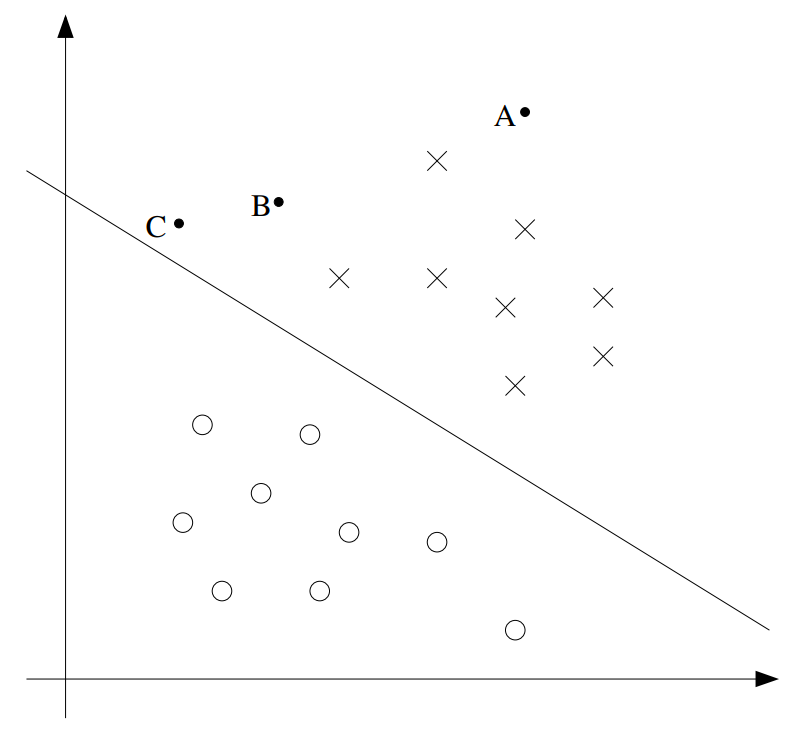
\includegraphics[width=0.5\linewidth]{figs/svm_hyperplane.png}
\end{figure}

注意到点 A 离决策边界非常远。如果要求预测 A 点的 $y$ 值,似乎应该非常确信那里 $y=1$。相反,点 C 离决策边界非常近,尽管它在决策边界预测 $y=1$ 的一侧,但决策边界的微小变化似乎很容易导致预测结果为 $y=0$。因此,在 A 点的预测比在 C 点更确信。点 B 介于这两种情况之间,更广泛地说,可以看出,如果一个点离分隔超平面很远,那么预测可能会更确信。同样,非正式地认为,如果给定一个训练集,能够找到一个决策边界,使得在训练样本上做出所有正确且确信(即远离决策边界)的预测,那将是很好的。稍后将使用几何间隔的概念来形式化这个想法。

\section{符号 (选读)}

为了更容易讨论 SVM,首先需要引入一种新的符号来讨论分类。将考虑一个二元分类问题的线性分类器,其标签为 $y$,特征为 $x$。从现在开始,使用 $y \in \{-1, 1\}$(而不是 $\{0, 1\}$)来表示类别标签。此外,不再使用向量 $\theta$ 来参数化线性分类器,而是使用参数 $w, b$,并将分类器写为
\[
    h_{w,b}(x) = g(w^T x + b).
\]
这里,$g(z) = 1$ 如果 $z \ge 0$,否则 $g(z) = -1$。这种“$w, b$”符号允许将截距项 $b$ 与其他参数分开处理(还放弃了之前让 $x_0 = 1$ 成为输入特征向量中的额外坐标的约定)。因此,$b$ 扮演着之前 $\theta_0$ 的角色,而 $w$ 扮演着 $[\theta_1 \dots \theta_d]^T$ 的角色。

还注意到,根据上面 $g$ 的定义,分类器将直接预测 1 或 -1(参见感知器算法),而无需先经过估计 $p(y=1)$ 的中间步骤(这是逻辑回归所做的)。

\section{函数间隔与几何间隔 (选读)}\label{sec:6.3}

现在将函数间隔和几何间隔的概念形式化。给定一个训练样本 $(x^{(i)}, y^{(i)})$,定义 $(w,b)$ 相对于训练样本的\textbf{函数间隔 (functional margin)}为
\[
    \hat{\gamma}^{(i)} = y^{(i)}(w^T x^{(i)} + b).
\]
注意,如果 $y^{(i)} = 1$,那么为了使函数间隔大(即,预测是确信且正确的),需要 $w^T x^{(i)} + b$ 是一个大的正数。相反,如果 $y^{(i)} = -1$,那么为了使函数间隔大,需要 $w^T x^{(i)} + b$ 是一个大的负数。此外,如果 $y^{(i)}(w^T x^{(i)} + b) > 0$,那么对这个样本的预测是正确的。(自己验证一下。)因此,大的函数间隔表示确信且正确的预测。

对于上面给出的 $g$ 选择的线性分类器(取值在 $\{-1, 1\}$ 中),然而函数间隔有一个性质使得它不是一个非常好的置信度度量。考虑 $g$ 的选择,注意到如果将 $w$ 替换为 $2w$,将 $b$ 替换为 $2b$,那么由于 $g(w^T x + b) = g(2w^T x + 2b)$,这根本不会改变 $h_{w,b}(x)$。也就是说,$g$,以及因此 $h_{w,b}(x)$,仅取决于 $w^T x + b$ 的符号,而不是大小。然而,将 $(w,b)$ 替换为 $(2w, 2b)$ 也会导致函数间隔乘以 2。因此,似乎通过利用缩放 $w$ 和 $b$ 的自由度,可以在不改变任何有意义的东西的情况下使函数间隔任意大。直观地说,因此施加某种归一化条件(例如 $||w||_2 = 1$)可能是有意义的;也就是说,可以将 $(w,b)$ 替换为 $(w/||w||_2, b/||w||_2)$,并改为考虑 $(w/||w||_2, b/||w||_2)$ 的函数间隔。稍后将回到这一点。

给定一个训练集 $S = \{(x^{(i)}, y^{(i)}); i = 1, \dots, n\}$,还定义 $(w,b)$ 相对于 $S$ 的函数间隔为各个训练样本的函数间隔中的最小值。用 $\hat{\gamma}$ 表示,因此可以写为:
\[
    \hat{\gamma} = \min_{i=1,\dots,n} \hat{\gamma}^{(i)}.
\]

接下来,讨论\textbf{几何间隔 (geometric margins)}。考虑下面的图:

\begin{figure}[H]
    \centering
    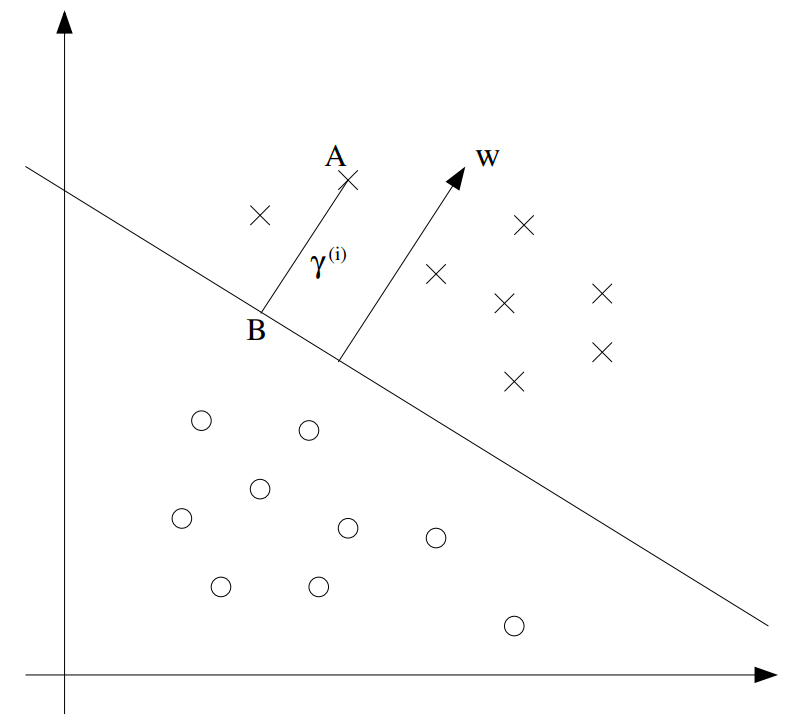
\includegraphics[width=0.5\linewidth]{figs/svm_geo_margin.png}
\end{figure}

图中显示了与 $(w,b)$ 对应的决策边界以及向量 $w$。注意 $w$ 与分隔超平面正交(呈 $90^\circ$ 角)(您应该说服自己确实如此)。 考虑 A 点,它代表标记为 $y^{(i)}=1$ 的某个训练样本的输入 $x^{(i)}$。它到决策边界的距离 $\gamma^{(i)}$ 由线段 AB 给出。

如何找到 $\gamma^{(i)}$ 的值?$w/||w||$ 是一个单位长度向量,方向与 $w$ 相同。由于 A 代表 $x^{(i)}$,因此可以发现点 B 由 $x^{(i)} - \gamma^{(i)} \cdot w/||w||$ 给出。但这个点位于决策边界上,而决策边界上的所有点 $x$ 都满足方程 $w^T x + b = 0$。因此,
\[
    w^T \left( x^{(i)} - \gamma^{(i)} \frac{w}{||w||} \right) + b = 0.
\]
解出 $\gamma^{(i)}$ 得到
\[
    \gamma^{(i)} = \frac{w^T x^{(i)} + b}{||w||} = \left(\frac{w}{||w||}\right)^T x^{(i)} + \frac{b}{||w||}.
\]
这是针对图中 A 点处正训练样本的情况推导的,其中位于决策边界的“正”侧是好的。更一般地,定义 $(w,b)$ 相对于训练样本 $(x^{(i)}, y^{(i)})$ 的几何间隔为
\[
    \gamma^{(i)} = y^{(i)} \left( \left(\frac{w}{||w||}\right)^T x^{(i)} + \frac{b}{||w||} \right).
\]

注意,如果 $||w|| = 1$,那么函数间隔等于几何间隔——这提供了一种关联这两种不同间隔概念的方式。此外,几何间隔对于参数的缩放是不变的;也就是说,如果用 $2w$ 和 $2b$ 替换 $w$ 和 $b$,那么几何间隔不会改变。这在后面会很有用。具体来说,由于参数缩放的这种不变性,在试图拟合 $w$ 和 $b$ 到训练数据时,可以在不改变任何重要内容的情况下对 $w$ 施加任意缩放约束;例如,可以要求 $||w|| = 1$,或者 $|w_1| = 5$,或者 $|w_1 + b| + |w_2| = 2$,并且这些都可以通过缩放 $w$ 和 $b$ 简单地满足。

最后,给定一个训练集 $S = \{(x^{(i)}, y^{(i)}); i = 1, \dots, n\}$,还定义 $(w,b)$ 相对于 $S$ 的几何间隔为各个训练样本的几何间隔中的最小值:
\[
    \gamma = \min_{i=1,\dots,n} \gamma^{(i)}.
\]

\section{最优间隔分类器 (选读)}

给定一个训练集,从之前的讨论来看,一个自然期望是找到一个决策边界,使其几何间隔最大化,因为这将反映一组在训练集上非常确信的预测,并且其能很好地“拟合”训练数据。具体来说,这将产生一个分类器,它用一个“间隔”(几何间隔)来分隔正训练样本和负训练样本。

目前,假设给定一个线性可分的训练集;也就是说,可以通过某个分隔超平面来分隔正样本和负样本。如何找到能实现最大几何间隔的那个呢?可以提出以下优化问题:
\begin{align*}
    \max_{\gamma, w, b} \quad &\gamma\\
    \text{s.t.} & y^{(i)}(w^T x^{(i)} + b) \ge \gamma, \quad i = 1, \dots, n\\
    &||w|| = 1.
\end{align*}
也就是说,希望最大化 $\gamma$,约束条件是每个训练样本的函数间隔至少为 $\gamma$。此外,$||w|| = 1$ 约束确保了函数间隔等于几何间隔,因此也保证了所有几何间隔至少为 $\gamma$。因此,解决这个问题将得到 $(w,b)$,使其相对于训练集具有最大的可能几何间隔。

如果能解决上面的优化问题,任务就完成了。但是,“$||w|| = 1$” 是一个令人讨厌的(非凸)约束,并且这种问题肯定不是标准优化软件可以解决的格式。因此,尝试将问题转换为更友好的形式。考虑:
\begin{align*}
    \max_{\gamma, w, b} \quad &\frac{\hat\gamma}{||w||}\\
    \text{s.t.} \quad & y^{(i)}(w^T x^{(i)} + b) \ge \hat\gamma, \quad i = 1, \dots, n
\end{align*}
这里,要最大化 $\hat{\gamma}/||w||$,约束条件是所有函数间隔至少为 $\hat{\gamma}$。由于几何间隔和函数间隔通过 $\gamma = \hat{\gamma}/||w||$ 相关,这将得到想要的答案。此外,摆脱了不喜欢的 $||w|| = 1$ 约束。缺点是现在有一个令人讨厌的(还是非凸的)目标函数 $\frac{\hat{\gamma}}{||w||}$;而且,仍然没有现成的软件可以解决这种形式的优化问题。

再想想。回想之前关于可以在不改变任何内容的情况下对 $w$ 和 $b$ 添加任意缩放约束的讨论。这是现在要使用的关键思想。引入缩放约束,使得 $(w,b)$ 相对于训练集的函数间隔必须为 1:
\[
    \hat{\gamma} = 1.
\]
由于将 $w$ 和 $b$ 乘以某个常数会导致函数间隔也乘以相同的常数,这确实是一个缩放约束,并且可以通过缩放 $w, b$ 来满足。将其代入上面的问题,并注意到最大化 $\hat{\gamma}/||w|| = 1/||w||$ 等价于最小化 $||w||^2$,现在有了以下优化问题:
\begin{align*}
    \min_{w, b} \quad &\frac{1}{2}||w||^2\\
    \text{s.t.} \quad & y^{(i)}(w^T x^{(i)} + b) \ge \hat\gamma, \quad i = 1, \dots, n
\end{align*}

现在已经将问题转换成可以有效求解的形式。上述问题是一个具有凸二次目标函数和线性约束的优化问题。其解给出了\textbf{最优间隔分类器 (optimal margin classifier)}。可以使用商用二次规划(QP)代码来解决此优化问题\footnote{您可能熟悉线性规划,它解决具有目标函数和约束均是线性的优化问题。QP 软件也广泛可用,它允许具有凸二次目标函数和线性约束。}。

虽然可以称此问题已解决,但下文会进一步讨论拉格朗日对偶性。这将导出优化问题的对偶形式,使得我们可以应用核函数让最优间隔分类器在极高维空间中高效工作。对偶形式还将允许推导出一种求解上述优化问题的高效算法,该算法通常比通用 QP 软件表现更好。

\section{拉格朗日对偶性 (选读)}

暂时搁置支持向量机和最大间隔分类器,讨论如何解决带约束的优化问题。

考虑以下形式的问题:
\begin{align*}
    \min_w \quad &f(w)\\
    \text{s.t.} \quad &h_i(w)=0,\quad i=1,\dots,l.
\end{align*}
一些读者可能还记得如何使用拉格朗日乘数法来解决此问题。(如果以前没有见过,不用担心。)在此方法中,定义\textbf{拉格朗日函数 (Lagrangian)} 为
\[
    \mathcal{L}(w, \beta) = f(w) + \sum_{i=1}^l \beta_i h_i(w)
\]
这里,$\beta_i$ 称为\textbf{拉格朗日乘数 (Lagrange multipliers)}。然后找到 $\mathcal{L}$ 的偏导数并将其设为零:
\[
    \frac{\partial \mathcal{L}}{\partial w_i} = 0; \quad \frac{\partial \mathcal{L}}{\partial \beta_i} = 0,
\]
并求解 $w$ 和 $\beta$。

在本节中,将此推广到可能包含不等式约束和等式约束的优化问题。由于时间限制,无法在本课程中充分论述拉格朗日对偶性理论\footnote{对学习更多关于此主题感兴趣的读者,建议阅读,例如,R. T. Rockafeller (1970), Convex Analysis, Princeton University Press.},但将给出主要思想和结果,并将其应用于最优间隔分类器的优化问题。

考虑以下问题,将其称为\textbf{原始 (primal)} 优化问题:

\begin{align*}
    \min_w \quad &f(w)\\
    \text{s.t.} \quad &g_i(w)\leq 0, \quad i=1,\dots,k\\
    \quad &h_i(w)=0, \quad i=1,\dots,l.
\end{align*}
为了解决它,首先定义\textbf{广义拉格朗日函数 (generalized Lagrangian)}:
\[
    \mathcal{L}(w, \alpha, \beta) = f(w) + \sum_{i=1}^k \alpha_i g_i(w) + \sum_{i=1}^l \beta_i h_i(w).
\]
这里,$\alpha_i$ 和 $\beta_i$ 是拉格朗日乘数。考虑以下量
\[
    \theta_{\mathcal{P}}(w) = \max_{\alpha, \beta: \alpha_i \ge 0} \mathcal{L}(w, \alpha, \beta).
\]
这里,下标 “$\mathcal{P}$” 代表 “原始”。给定某个 $w$。如果 $w$ 违反任何原始约束(即,对于某个 $i$,要么 $g_i(w) > 0$ 要么 $h_i(w) \ne 0$),那么应该能够验证
\begin{align}
    \theta_{\mathcal{P}}(w) &= \max_{\alpha, \beta: \alpha_i \ge 0} f(w) + \sum_{i=1}^k \alpha_i g_i(w) + \sum_{i=1}^l \beta_i h_i(w) \label{eq:6.1} \\
    &= \infty. \label{eq:6.2}
\end{align}
反之,如果约束对于某个特定的 $w$ 值确实满足,那么 $\theta_{\mathcal{P}}(w) = f(w)$。因此,
\[
    \theta_{\mathcal{P}}(w) = \begin{cases} f(w) & \text{若 } w \text{ 满足原始约束} \\ \infty & \text{其他情况}. \end{cases}
\]
因此,对于满足原始约束的所有 $w$ 值,$\theta_{\mathcal{P}}$ 取与问题中目标函数相同的值,如果违反约束,则为正无穷大。因此,如果考虑最小化问题
\[
    \min_w \theta_{\mathcal{P}}(w) = \min_w \max_{\alpha, \beta: \alpha_i \ge 0} \mathcal{L}(w, \alpha, \beta),
\]
可以看出它与原始问题相同(即,具有与原始问题相同的解)。为了后续使用,还将目标函数的最优值定义为 $p^* = \min_w \theta_{\mathcal{P}}(w)$;将其称为原始问题的\textbf{值 (value)}。

现在,考察一个稍微不同的问题。定义
\[
    \theta_{\mathcal{D}}(\alpha, \beta) = \min_w \mathcal{L}(w, \alpha, \beta).
\]
这里,下标 “$\mathcal{D}$” 代表 “对偶”。注意,在 $\theta_{\mathcal{P}}$ 的定义中,关于 $\alpha, \beta$ 进行优化(最大化),而这里关于 $w$ 进行最小化。

现在可以提出\textbf{对偶 (dual)} 优化问题:
\[
    \max_{\alpha, \beta: \alpha_i \ge 0} \theta_{\mathcal{D}}(\alpha, \beta) = \max_{\alpha, \beta: \alpha_i \ge 0} \min_w \mathcal{L}(w, \alpha, \beta).
\]
这与上面显示的原始问题完全相同,只是 “max” 和 “min” 的顺序现在交换了。将对偶问题目标函数的最优值定义为 $d^* = \max_{\alpha, \beta: \alpha_i \ge 0} \theta_{\mathcal{D}}(w)$。

原始问题和对偶问题如何关联?很容易证明
\[
    d^* = \max_{\alpha, \beta: \alpha_i \ge 0} \min_w \mathcal{L}(w, \alpha, \beta) \le \min_w \max_{\alpha, \beta: \alpha_i \ge 0} \mathcal{L}(w, \alpha, \beta) = p^*.
\]
(您应该自己证明这一点;这源自函数 “max min” 总是小于或等于 “min max”。)然而,在某些条件下,将有
\[
    d^* = p^*,
\]
这样就可以求解对偶问题来代替原始问题。来看看这些条件是什么。

假设 $f$ 和 $g_i$ 是凸函数\footnote{当 $f$ 具有 Hessian 矩阵时,当且仅当 Hessian 矩阵是半正定时,它是凸的;类似地,所有线性(和仿射)函数也是凸的。(函数 $f$ 也可以在不可微的情况下是凸的,但这里不需要那些更一般的凸性定义。)},并且 $h_i$ 是仿射函数\footnote{即,存在 $a_i, b_i$,使得 $h_i(w) = a_i^T w + b_i$。“仿射”的意思与线性相同,只是允许额外的截距项 $b_i$。}。进一步假设约束 $g_i$ 是(严格)可行的;这意味着存在某个 $w$ 使得对于所有 $i$,都有 $g_i(w) < 0$。

在上述假设下,必然存在 $w^*, \alpha^*, \beta^*$,使得 $w^*$ 是原始问题的解,$\alpha^*, \beta^*$ 是对偶问题的解,并且 $p^* = d^* = \mathcal{L}(w^*, \alpha^*, \beta^*)$。此外,$w^*, \alpha^*$ 和 $\beta^*$ 满足 \textbf{Karush-Kuhn-Tucker (KKT) 条件},如下:
\begin{align}
    \frac{\partial}{\partial w_i} \mathcal{L}(w^*, \alpha^*, \beta^*) &= 0, \quad i = 1, \dots, d \label{eq:6.3} \\
    \frac{\partial}{\partial \beta_i} \mathcal{L}(w^*, \alpha^*, \beta^*) &= 0, \quad i = 1, \dots, l \label{eq:6.4} \\
    \alpha_i^* g_i(w^*) &= 0, \quad i = 1, \dots, k \label{eq:6.5} \\
    g_i(w^*) &\le 0, \quad i = 1, \dots, k \label{eq:6.6} \\
    \alpha^* &\ge 0, \quad i = 1, \dots, k \label{eq:6.7}
\end{align}
此外,如果某个 $w^*, \alpha^*, \beta^*$ 满足 KKT 条件,那么它也是原始问题和对偶问题的解。

请注意方程 (\ref{eq:6.5}),它被称为 KKT \textbf{对偶互补性条件 (dual complementarity)}。具体来说,这意味着如果 $\alpha_i^* > 0$,那么 $g_i(w^*) = 0$。(即,“$g_i(w) \le 0$” 约束是\textbf{活跃 (active)} 的,意味着它以等式而不是不等式成立。)稍后,这将是证明 SVM 只有少量“支持向量”的关键;KKT 对偶互补性条件也将为讨论 SMO 算法时提供收敛性测试。

\section{最优间隔分类器:对偶形式 (选读)}

\textcolor{blue}{注:}\textit{优化问题 \eqref{eq:primal_opt} 与优化问题 \eqref{eq:dual_opt} 的等价性,以及方程 \eqref{eq:dual_relation} 中原始变量和对偶变量之间的关系是本节最重要的收获。}

前面,提出了以下寻找最优间隔分类器的问题(原始)优化问题:
\begin{align}
    \min_{w,b} \quad &\frac{1}{2}\|w\|^2 \label{eq:primal_opt}\\
    \text{s.t.} \quad &y^{(i)}(w^T x^{(i)} + b) \ge 1, \quad i = 1, \dots, n \notag
\end{align}
可以将约束写成
\[
    g_i(w) = -y^{(i)}(w^T x^{(i)} + b) + 1 \le 0.
\]
每个训练样本都有一个这样的约束。注意,根据 KKT 对偶互补性条件,只有当训练样本的功能间隔恰好等于 1 时(即,对应于满足等式 $g_i(w) = 0$ 的约束),$\alpha_i$ 才大于 0。考虑下图中,其中实线表示最大间隔分离超平面。

\begin{figure}[H]
    \centering
    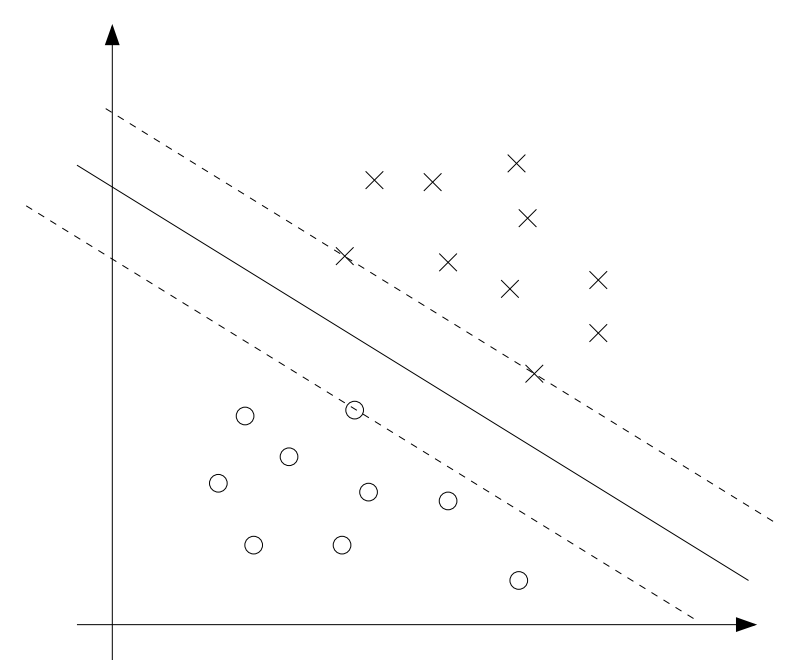
\includegraphics[width=0.5\linewidth]{figs/svm_max_margin.png}
\end{figure}

间隔最小的点恰好是离决策边界最近的点;在这里,这三个点(一个负样本和两个正样本)位于平行于决策边界的虚线上。因此,只有这三个 $\alpha_i$(即,对应于这三个训练样本的 $\alpha_i$)在最优解处非零。这三个点被称为该问题中的\textbf{支持向量 (support vectors)}。支持向量的数量可以远小于训练集的大小,这一事实将在稍后有用。

接下来,在推导对偶形式问题时,需要注意的一个关键思想是,我们将尝试仅使用内积 $\langle x^{(i)}, x^{(j)} \rangle$(将其视为输入特征空间中点之间的 $(x^{(i)})^T x^{(j)}$)来编写算法。算法能够用这些内积表达的事实是应用核技巧的关键。

构建优化问题的拉格朗日函数为:
\begin{equation}
    \mathcal{L}(w, b, \alpha) = \frac{1}{2}\|w\|^2 - \sum_{i=1}^n \alpha_i [y^{(i)}(w^T x^{(i)} + b) - 1]. \label{eq:la_opt}
\end{equation}
注意,只有“$\alpha_i$”而没有“$\beta_i$”拉格朗日乘子,因为问题只有不等式约束。

继续推导问题的对偶形式。为此,需要首先对固定的 $\alpha$ 最小化 $\mathcal{L}(w, b, \alpha)$ 关于 $w$ 和 $b$,以得到 $\theta_D$。方法是将 $\mathcal{L}$ 关于 $w$ 和 $b$ 的导数设为零。得到:
\[
    \nabla_w \mathcal{L}(w, b, \alpha) = w - \sum_{i=1}^n \alpha_i y^{(i)} x^{(i)} = 0
\]
这意味着
\begin{equation}
    w = \sum_{i=1}^n \alpha_i y^{(i)} x^{(i)}. \label{eq:dual_relation}
\end{equation}
关于 $b$ 的导数,得到
\begin{equation}
    \frac{\partial}{\partial b} \mathcal{L}(w, b, \alpha) = \sum_{i=1}^n \alpha_i y^{(i)} = 0. \label{eq:6.11}
\end{equation}
将式 \eqref{eq:dual_relation} 中 $w$ 的定义代入拉格朗日函数 \eqref{eq:la_opt},并简化,得到
\[
    \mathcal{L}(w, b, \alpha) = \sum_{i=1}^n \alpha_i - \frac{1}{2} \sum_{i,j=1}^n y^{(i)} y^{(j)} \alpha_i \alpha_j (x^{(i)})^T x^{(j)} - b \sum_{i=1}^n \alpha_i y^{(i)}.
\]
但根据式 \eqref{eq:6.11},最后一项必须为零,所以得到
\[
    \mathcal{L}(w, b, \alpha) = \sum_{i=1}^n \alpha_i - \frac{1}{2} \sum_{i,j=1}^n y^{(i)} y^{(j)} \alpha_i \alpha_j (x^{(i)})^T x^{(j)}.
\]
回想一下,通过对 $\mathcal{L}$ 关于 $w$ 和 $b$ 进行最小化,得到了上面的方程。将其与约束 $\alpha_i \ge 0$(始终存在)和约束 \eqref{eq:6.11} 结合,得到以下对偶优化问题:
\begin{align}
    \max_\alpha \quad &W(\alpha) = \sum_{i=1}^n \alpha_i - \frac{1}{2} \sum_{i,j=1}^n y^{(i)} y^{(j)} \alpha_i \alpha_j \langle x^{(i)}, x^{(j)} \rangle \label{eq:dual_opt} \\
    \text{s.t.} \quad & \alpha_i \ge 0, \quad i=1,\dots,n \notag\\
     & \sum_{i=1}^n \alpha_i y^{(i)} = 0. \notag
\end{align}

还应该能够验证 $p^* = d^*$ 所需的条件以及 KKT 条件(式 \eqref{eq:6.3}-\eqref{eq:6.7})在我们的优化问题里确实满足。因此,可以通过求解对偶问题来求解原问题。具体而言,在上述对偶问题中,这是一个最大化问题,其中的参数是 $\alpha_i$。稍后将讨论用于求解对偶问题的具体算法,但如果确实能够求解它(即找到使 $W(\alpha)$ 最大化且满足约束的 $\alpha$),那么就可以使用式 \eqref{eq:dual_relation} 回过头来找到最优的 $w$ 作为 $\alpha$ 的函数。找到 $w^*$ 后,通过考虑原问题,也很容易找到截距项 $b$ 的最优值,如下所示:
\begin{equation}
    b^* = - \frac{\max_{i:y^{(i)}=-1} w^{*T} x^{(i)} + \min_{i:y^{(i)}=1} w^{*T} x^{(i)}}{2}. \label{eq:6.13}
\end{equation}
(可以自行验证一下此处的正确性。)

继续之前,再仔细看看式 \eqref{eq:dual_relation},它给出了 $w$ 的最优值(以最优 $\alpha$ 表示)。假设已经用训练集拟合了模型参数,现在想对新的输入点 $x$ 进行预测。然后计算 $w^T x + b$,并且当且仅当该值大于零时预测 $y=1$。但是使用 \eqref{eq:dual_relation},该值也可以写成:
\begin{align}
    w^T x + b &= \left(\sum_{i=1}^n \alpha_i y^{(i)} x^{(i)}\right)^T x + b \\
    &= \sum_{i=1}^n \alpha_i y^{(i)} \langle x^{(i)}, x \rangle + b. \label{eq:6.15}
\end{align}
因此,如果找到了 $\alpha_i$,为了进行预测,必须计算一个仅取决于 $x$ 与训练集中的点之间的内积的值。此外,之前已经看到,除了支持向量对应的 $\alpha_i$ 外,其他所有 $\alpha_i$ 都将为零。因此,上面求和中的许多项将为零,并且实际上只需要计算 $x$ 与支持向量(通常数量很少)之间的内积,以便计算 \eqref{eq:6.15} 并进行预测。

通过研究优化问题的对偶形式,对问题的结构获得了重要的见解,并且还能够仅以内积形式编写整个算法。在下一节中,将利用这一特性将核函数应用于分类问题。由此产生的算法,\textbf{支持向量机 (support vector machines)},将能够在非常高维的空间中高效学习。

\section{正则化与非线性可分情况 (选读)}

目前为止介绍的支持向量机推导假设数据是线性可分的。虽然通过 $\phi$ 将数据映射到高维特征空间通常会增加数据可分的可能性,但不能保证总是如此。此外,在某些情况下,找到一个分离超平面并非完全符合期望,因为它可能对离群点敏感。例如,下面左图显示了一个最优间隔分类器,当在左上方区域(右图)添加一个离群点时,决策边界会发生剧烈变化,并且得到的分类器的间隔会小得多。

\begin{figure}[H]
    \centering
    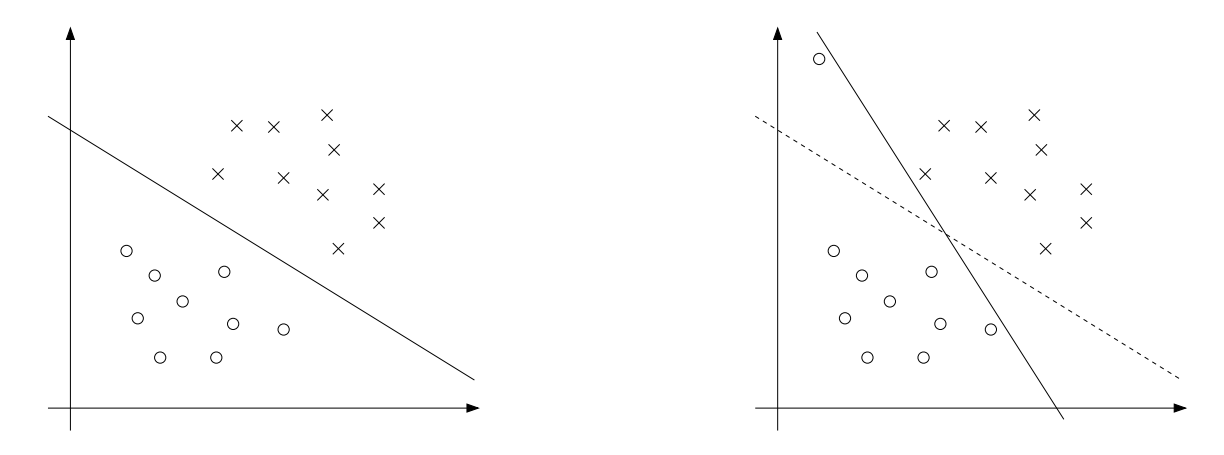
\includegraphics[width=0.93\linewidth]{figs/svm_regularization.png}
\end{figure}

为了使算法也适用于非线性可分数据集并降低对离群点的敏感度,我们重新构建了优化问题(使用 $\ell_1$ \textbf{正则化 (regularization)}),如下所示:
\begin{align*}
    \min_{\gamma,w,b} \quad& \frac{1}{2}\|w\|^2 + C \sum_{i=1}^n \xi_i \\
    \text{s.t.} \quad& y^{(i)}(w^T x^{(i)} + b) \ge 1 - \xi_i, \quad i=1,\dots,n \\
    &\xi_i \ge 0, \quad i=1,\dots,n.
\end{align*}
因此,现在允许存在(函数)间隔小于 1 的样本,如果一个样本的函数间隔为 $1-\xi_i$(其中 $\xi_i > 0$),那么目标函数会增加 $C\xi_i$ 的代价。参数 $C$ 控制了两个目标之间的相对权重:使 $\|w\|^2$ 小(如前面所述,这会使间隔大)以及确保大多数样本的函数间隔至少为 1。

与之前一样,可以构建拉格朗日函数:
\[
    \mathcal{L}(w, b, \xi, \alpha, r) = \frac{1}{2} w^T w + C \sum_{i=1}^n \xi_i - \sum_{i=1}^n \alpha_i [y^{(i)}(w^T x^{(i)} + b) - 1 + \xi_i] - \sum_{i=1}^n r_i \xi_i.
\]
这里,$\alpha_i$ 和 $r_i$ 是拉格朗日乘子(约束为 $\ge 0$)。将不再详细推导对偶问题,但在像之前一样将关于 $w$ 和 $b$ 的导数设为零,然后代入并简化后,得到问题的对偶形式:
\begin{align*}
    \max{\alpha} \quad& W(a)=\sum_{i=1}^{n}a_i - \frac12 \sum_{i,j=1}^n y^{(i)}y^{(j)}\alpha_i\alpha_j\langle x^{(i)}x^{(j)} \rangle \\
    \text{s.t.} \quad& 0\le \alpha_i\le C, \quad i=1,\dots,n \\
    &\sum_{i=1}^{n}\alpha_i y^{(i)}=0.
\end{align*}

与之前一样,同样有 $w$ 可以表示为 $\alpha_i$ 的函数,如式 \eqref{eq:dual_relation} 所示,因此在求解对偶问题后,可以继续使用式 \eqref{eq:6.15} 进行预测。注意,令人惊讶的是,在添加 $\ell_1$ 正则化后,对偶问题唯一的改变是原先的约束 $0 \le \alpha_i$ 现在变成了 $0 \le \alpha_i \le C$。对 $b^*$ 的计算也必须进行修改(式 \eqref{eq:6.13} 不再有效);请参阅下一节中的注释或 Platt 的论文。

此外,KKT 对偶互补条件(在下一节中将用于测试 SMO 算法的收敛性)为:
\begin{align}
    \alpha_i = 0 &\Rightarrow y^{(i)}(w^T x^{(i)} + b) \ge 1 \label{eq:6.16} \\
    \alpha_i = C &\Rightarrow y^{(i)}(w^T x^{(i)} + b) \le 1 \label{eq:6.17} \\
    0 < \alpha_i < C &\Rightarrow y^{(i)}(w^T x^{(i)} + b) = 1. \label{eq:6.18}
\end{align}
现在,剩下的就是给出一个实际求解对偶问题的算法,这将在下一节中进行。

\section{SMO 算法 (选读)}

序列最小化 (sequential minimal optimization, SMO) 算法,由 John Platt 提出,提供了一种有效求解由 SVM 推导得到的对偶问题的方法。部分是为了引出 SMO 算法,部分是因为它本身很有趣,让我们先再进行一次岔开讨论,谈谈坐标上升算法。

\subsection{坐标上升}

考虑尝试求解无约束优化问题
\[
    \max_\alpha W(\alpha_1, \alpha_2, \dots, \alpha_n).
\]
这里,将 $W$ 视为参数 $\alpha_i$ 的某个函数,暂时忽略这个问题与支持向量机之间的任何关系。之前已经见过两种优化算法:梯度上升和牛顿法。这里要考虑的新算法称为\textbf{坐标上升 (coordinate ascent)}:

循环直到收敛: \{

    $\quad\quad$对于 $i=1,\dots,n,$ \{
        \[
            \alpha_i := \arg\max_{\hat a_i} W(\alpha_1,\dots,\alpha_{i-1},\hat{\alpha_i},\alpha_{i+1},\dots,\alpha_n).
        \]
        
    $\quad\quad$\}

\}

因此,在该算法的最内层循环中,将固定除某个 $\alpha_i$ 之外的所有变量,并仅针对参数 $\alpha_i$ 重新优化 $W$。在该方法此处介绍的版本中,内层循环按 $\alpha_1, \alpha_2, \dots, \alpha_n, \alpha_1, \alpha_2, \dots$ 的顺序重新优化变量。(更复杂的版本可以选择其他顺序;例如,可以根据期望哪个变量能使 $W(\alpha)$ 增加最大来选择下一个要更新的变量。)

当函数 $W$ 的形式恰好使得内层循环中的 “arg max” 可以高效执行时,坐标上升可以是一个相当高效的算法。这里是坐标上升算法的一个图例:

\begin{figure}[H]
    \centering
    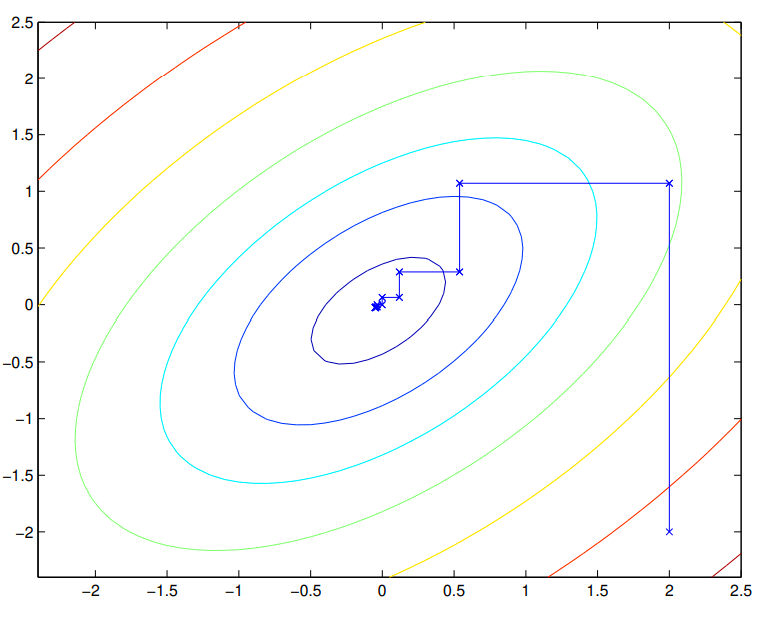
\includegraphics[width=0.5\linewidth]{figs/svm_coordinate_ascent.png}
\end{figure}


图中的椭圆是我们想要优化的二次函数的等高线。坐标上升从 $(2, -2)$ 初始化,图中绘制了它通往全局最大值的路径。注意到在每一步,坐标上升都沿着与一个坐标轴平行的方向前进,因为每次只优化一个变量。

\subsection{SMO}

通过概述 SMO 算法的推导来结束对支持向量机的讨论。

这是我们想要解决的(对偶)优化问题:
\begin{align}
    \max_\alpha \quad &W(\alpha) = \sum_{i=1}^n \alpha_i - \frac{1}{2} \sum_{i,j=1}^n y^{(i)} y^{(j)} \alpha_i \alpha_j \langle x^{(i)}, x^{(j)} \rangle \\
    \text{s.t.} \quad &0 \le \alpha_i \le C, \quad i=1,\dots,n \label{eq:6.20}\\
    &\sum_{i=1}^n \alpha_i y^{(i)} = 0. \label{eq:6.21}
\end{align}

假设我们有一组满足约束 (\eqref{eq:6.20}-\eqref{eq:6.21}) 的 $\alpha_i$。现在,假设我们固定 $\alpha_2, \dots, \alpha_n$,并进行坐标上升步骤,关于 $\alpha_1$重新优化目标函数。能取得任何进展吗?答案是否定的,因为约束 \eqref{eq:6.21} 确保
\[
    \alpha_1 y^{(1)} = - \sum_{i=2}^n \alpha_i y^{(i)}.
\]

或者,通过将两边乘以 $y^{(1)}$,我们等价地得到
\[
    \alpha_1 = -y^{(1)} \sum_{i=2}^n \alpha_i y^{(i)}.
\]
(这一步使用了 $y^{(1)} \in \{-1, 1\}$ 的事实,因此 $(y^{(1)})^2 = 1$。)因此,$\alpha_1$ 完全由其他 $\alpha_i$ 确定,如果固定 $\alpha_2, \dots, \alpha_n$,那么在不违反优化问题中的约束 \eqref{eq:6.21} 的情况下,无法对 $\alpha_1$ 进行任何改变。

因此,如果想要更新一些 $\alpha_i$,必须同时更新至少两个,以便保持约束得到满足。这促使了 SMO 算法,其简单来说就是以下步骤:

\begin{samepage}
重复直到收敛 \{
\vspace{-0.5em}
\begin{enumerate}
\setlength{\itemindent}{2em}
    \item 选择一对 $\alpha_i$ 和 $\alpha_j$ 进行下一次更新(使用启发式方法来选择能够最大程度接近全局最大值的两个变量)。
    \item 在保持所有其他 $\alpha_k$ ($k \ne i, j$) 固定的情况下,重新优化 $W(\alpha)$ 关于 $\alpha_i$ 和 $\alpha_j$。
\end{enumerate}
$\quad\quad$\}
\end{samepage}

为了测试该算法的收敛性,可以检查 KKT 条件(式 \eqref{eq:6.16}-\eqref{eq:6.18})是否在某个 $\textit{容差 (tol)}$ 内得到满足。这里,容差是收敛容差参数,通常设置为 0.01 到 0.001。(详细信息请参阅论文和伪代码。)

SMO 算法高效的关键原因在于 $\alpha_i, \alpha_j$ 的更新可以非常高效地计算。现在简要概述推导高效更新的主要思路。

假设当前有一组满足约束 (\eqref{eq:6.20}-\eqref{eq:6.21}) 的 $\alpha_i$,并且假设决定固定 $\alpha_3, \dots, \alpha_n$,并重新优化 $W(\alpha_1, \alpha_2, \dots, \alpha_n)$ 关于 $\alpha_1$ 和 $\alpha_2$(受约束限制)。根据 \eqref{eq:6.21},我们要求
\[
    \alpha_1 y^{(1)} + \alpha_2 y^{(2)} = - \sum_{i=3}^n \alpha_i y^{(i)}.
\]
由于右侧是固定的(因为已经固定了 $\alpha_3, \dots, \alpha_n$),可以将其记为某个常数 $\zeta$:
\begin{equation}
    \alpha_1 y^{(1)} + \alpha_2 y^{(2)} = \zeta. \label{eq:6.22}
\end{equation}
因此,可以将 $\alpha_1$ 和 $\alpha_2$ 的约束可视化如下:

\begin{figure}[H]
    \centering
    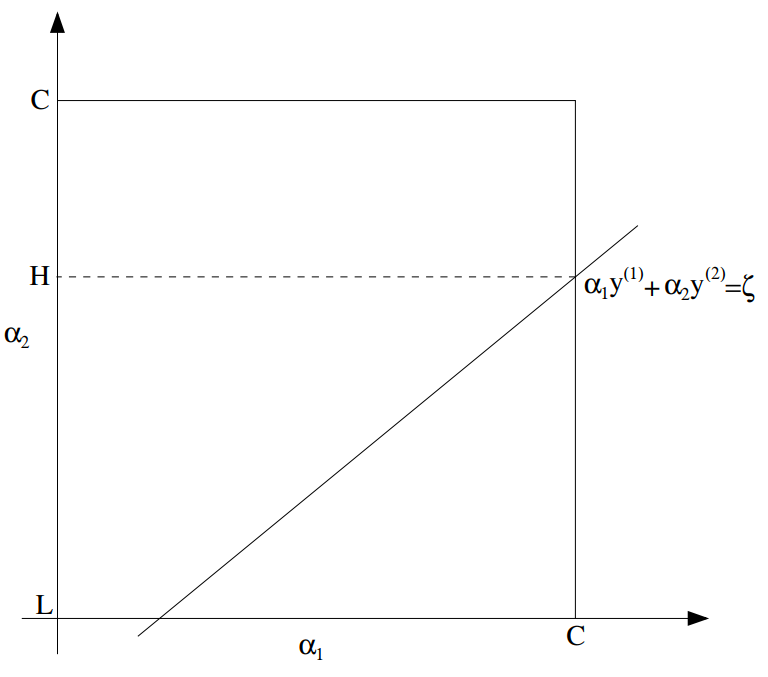
\includegraphics[width=0.5\linewidth]{figs/svm_smo_constraint.png}
\end{figure}

从约束 \eqref{eq:6.20} 中,我们知道 $\alpha_1$ 和 $\alpha_2$ 必须位于所示的盒子 $[0, C] \times [0, C]$ 内。还绘制了直线 $\alpha_1 y^{(1)} + \alpha_2 y^{(2)} = \zeta$,我们知道 $\alpha_1$ 和 $\alpha_2$ 必须位于该直线上。另外注意,从这些约束中,我们知道 $L \le \alpha_2 \le H$;否则,$(\alpha_1, \alpha_2)$ 无法同时满足盒子约束和直线约束。在此示例中,$L=0$。但这取决于直线 $\alpha_1 y^{(1)} + \alpha_2 y^{(2)} = \zeta$ 的样子,情况并非总是如此;更普遍地,对于 $\alpha_2$ 的允许值,会有一个下界 $L$ 和一个上界 $H$,以确保 $\alpha_1, \alpha_2$ 位于盒子 $[0, C] \times [0, C]$ 内。

使用方程 \eqref{eq:6.22},我们还可以将 $\alpha_1$ 写成 $\alpha_2$ 的函数:
\[
    \alpha_1 = (\zeta - \alpha_2 y^{(2)}) y^{(1)}.
\]
(请自行验证此推导;我们再次使用了 $y^{(1)} \in \{-1, 1\}$ 的事实,因此 $(y^{(1)})^2 = 1$。)因此,目标函数 $W(\alpha)$ 可以写成
\[
    W(\alpha_1, \alpha_2, \dots, \alpha_n) = W((\zeta - \alpha_2 y^{(2)}) y^{(1)}, \alpha_2, \dots, \alpha_n).
\]
将 $\alpha_3, \dots, \alpha_n$ 视为常数,您应该能够验证这是关于 $\alpha_2$ 的二次函数。也就是说,这也可以表示为 $a\alpha_2^2 + b\alpha_2 + c$ 的形式,其中 $a, b, c$ 是适当的常数。如果忽略“盒子”约束 \eqref{eq:6.20}(或等价地,忽略 $L \le \alpha_2 \le H$),那么我们可以通过将其导数设为零并求解来轻松最大化此二次函数。我们将令 $\alpha_2^{\text{new,unclipped}}$ 表示由此产生的 $\alpha_2$ 值。您还应该能够说服自己,如果改为最大化关于 $\alpha_2$ 的 $W$,但受盒子约束限制,那么可以通过简单地取 $\alpha_2^{\text{new,unclipped}}$ 并将其“剪裁”到$[L, H]$ 区间内,得到
\[
    \alpha_2^{\text{new}} = \begin{cases}
        H & \text{若}\  \alpha_2^{\text{new,unclipped}} > H \\
        \alpha_2^{\text{new,unclipped}} & \text{若}\  L \le \alpha_2^{\text{new,unclipped}} \le H \\
        L & \text{若}\  \alpha_2^{\text{new,unclipped}} < L
    \end{cases}
\]
最后,找到 $\alpha_2^{\text{new}}$ 后,可以使用方程 \eqref{eq:6.22} 返回并找到 $\alpha_1^{\text{new}}$ 的最优值。

还有一些细节非常简单,但我们将留给您自己在 Platt 的论文中阅读:一个是用于选择下一个要更新的 $\alpha_i, \alpha_j$ 的启发式方法的选择;另一个是 SMO 算法运行时如何更新 $b$。
\part{深度学习}

\chapter{深度学习}\label{chapter:7}
现在让我们开始学习深度学习。在本部分中,将概述神经网络,讨论向量化,并讨论使用反向传播训练神经网络。

\section{使用非线性模型的监督学习}\label{sec:7.1}

在监督学习设置中(从输入 $x$ 预测 $y$),假设我们的模型/假设是 $h_\theta(x)$。过去的章节里考虑了 $h_\theta(x) = \theta^T x$(线性回归)或 $h_\theta(x) = \theta^T \phi(x)$(其中 $\phi(x)$ 是特征映射)的情况。这两个模型的共同点是它们在参数 $\theta$ 中是线性的。接下来,我们将考虑学习在参数 $\theta$ 和输入 $x$ 中都\textbf{非线性 (non-linear)}的一般模型族。最常见的非线性模型是神经网络,我们将在下一节开始定义。对于本节,将 $h_\theta(x)$ 视为抽象的非线性模型即可\footnote{如果您需要一个具体的例子,可以考虑模型 $h_\theta(x) = \theta_1^2 x_1^2 + \theta_2^2 x_2^2 + \dots + \theta_d^2 x_d^2$,尽管它不是神经网络。}。

假设 $\{(x^{(i)}, y^{(i)})\}_{i=1}^n$ 是训练样本。我们将定义非线性模型及其学习的损失/成本函数。

\subsection*{回归问题}

为简单起见,我们从输出是实数的情况开始,即 $y^{(i)} \in \mathbb{R}$,因此模型 $h_\theta(x)$ 也输出实数 $h_\theta(x) \in \mathbb{R}$。将学习第 $i$ 个样本 $(x^{(i)}, y^{(i)})$ 的最小二乘成本函数定义为
\begin{equation} \label{eq:7.1}
    J^{(i)}(\theta) = \frac{1}{2} (h_\theta(x^{(i)}) - y^{(i)})^2,
\end{equation}
数据集的均方成本函数定义为
\begin{equation} \label{eq:7.2}
    J(\theta) = \frac{1}{n} \sum_{i=1}^n J^{(i)}(\theta),
\end{equation}
这与线性回归中的定义相同,只是为了与约定一致,我们在成本函数前引入了常数 $1/n$。注意,将成本函数乘以一个标量不会改变成本函数的局部最小点或全局最小点。另请注意,尽管成本函数的形式也是均方损失,但 $h_\theta(x)$ 的参数化与线性回归的情况不同。在后文中,“损失”和“成本”这两个词会互换使用。

\subsection*{二元分类}
接下来定义二元分类的模型和损失函数。假设输入 $x \in \mathbb{R}^d$。令 $\bar{h}_\theta: \mathbb{R}^d \to \mathbb{R}$ 是一个参数化模型(逻辑线性回归中 $\theta^T x$ 的类比)。将输出 $\bar{h}_\theta(x) \in \mathbb{R}$ 称为 logit。类似于第 \ref{sec:2.1} 节,使用 logistic 函数 $g(\cdot)$ 将 logit $\bar{h}_\theta(x)$ 转换为概率 $h_\theta(x) \in [0, 1]$:
\begin{equation} \label{eq:7.3}
    h_\theta(x) = g(\bar{h}_\theta(x)) = 1 / (1 + \exp(-\bar{h}_\theta(x))).
\end{equation}
使用以下方式建模给定 $x$ 和 $\theta$ 的 $y$ 的条件分布:
\[
\begin{aligned}
    P(y = 1 \mid x; \theta) &= h_\theta(x) \\
    P(y = 0 \mid x; \theta) &= 1 - h_\theta(x)
\end{aligned}
\]
按照第 \ref{sec:2.1} 节中的相同推导并使用备注 \ref{remark:2.1.1} 中的推导,负对数似然损失函数等于:
\begin{equation} \label{eq:7.4}
    J^{(i)}(\theta) = -\log p(y^{(i)} \mid x^{(i)}; \theta) = \ell_{\text{logistic}}(\bar{h}_\theta(x^{(i)}), y^{(i)})
\end{equation}
如公式 \eqref{eq:7.2} 中所示,总损失函数也定义为对单个训练样本的损失函数的平均值,$J(\theta) = \frac{1}{n} \sum_{i=1}^n J^{(i)}(\theta)$。

\subsection*{多类别分类}
按照第 \ref{sec:2.3} 节,考虑响应变量 $y$ 可以取 $k$ 个值之一的分类问题,即 $y \in \{1, 2, \dots, k\}$。令 $\bar{h}_\theta: \mathbb{R}^d \to \mathbb{R}^k$ 是一个参数化模型。将输出 $\bar{h}_\theta(x) \in \mathbb{R}^k$ 称为 logits。每个 logit 对应于 $k$ 个类别之一的预测。类似于第 \ref{sec:2.3} 节,使用 softmax 函数将 logits $\bar{h}_\theta(x)$ 转换为一个非负且和为 1 的概率向量:
\begin{equation} \label{eq:7.5}
    P(y = j \mid x; \theta) = \frac{\exp(\bar{h}_\theta(x)_j)}{\sum_{s=1}^k \exp(\bar{h}_\theta(x)_s)},
\end{equation}
其中 $\bar{h}_\theta(x)_s$ 表示 $\bar{h}_\theta(x)$ 的第 $s$ 个坐标。
类似于第 \ref{sec:2.3} 节,单个训练样本 $(x^{(i)}, y^{(i)})$ 的损失函数是其负对数似然:
\begin{equation} \label{eq:7.6}
    J^{(i)}(\theta) = -\log p(y^{(i)} \mid x^{(i)}; \theta) = -\log \left( \frac{\exp(\bar{h}_\theta(x^{(i)})_{y^{(i)}})}{\sum_{s=1}^k \exp(\bar{h}_\theta(x^{(i)})_s)} \right).
\end{equation}
使用第 \ref{sec:2.3} 节的符号,可以简单地抽象地写成:
\begin{equation} \label{eq:7.7}
    J^{(i)}(\theta) = \ell_{\text{ce}}(\bar{h}_\theta(x^{(i)}), y^{(i)}).
\end{equation}
损失函数也定义为单个训练样本的损失函数的平均值,$J(\theta) = \frac{1}{n} \sum_{i=1}^n J^{(i)}(\theta)$。

还注意到,上述方法也可以推广到任何条件概率模型,其中有一个关于 $y$ 的指数族分布 Exponential-family$(y; \eta)$,其中 $\eta = \bar{h}_\theta(x)$ 是一个参数化的非线性函数 $x$。然而,最广泛的情况还是上面讨论的三种情况。

\subsection*{优化器 (SGD)}

通常使用梯度下降 (GD)、随机梯度下降 (SGD) 或其变体来优化损失函数 $J(\theta)$。 GD 的更新规则可以写为\footnote{回顾一下,如之前所定义,使用符号 “$a := b$” 表示一个操作 (在计算机程序中),其中将变量 $a$ 的值设置为 $b$。 换句话说,此操作用 $b$ 的值覆盖 $a$。 相比之下,当断言事实陈述 $a$ 的值等于 $b$ 的值时,将写成 “$a = b$”。}

\begin{equation}
    \theta := \theta - \alpha \nabla_\theta J(\theta)
    \label{eq:7.8}
\end{equation}
其中 $\alpha > 0$ 通常称为学习率或步长。 接下来,介绍一个新的 SGD (算法 \ref{algo:1}),它与前面所讲的略有不同。

\vspace{0.5em}
\begin{algorithm}[H]
    \SetAlgoNoLine
    \label{algo:1}
    \caption{随机梯度下降}
    超参数:学习率 $\alpha$,总迭代数 $n_\text{iter}$\\
    随机初始化 $\theta$\\
    \For{$i=1$ \KwTo $n_\text{iter}$}{
        从 $\{1,\dots,n\}$ 中均匀采样一个 $j$,然后更新 $\theta$
        \begin{equation}\label{eq:7.9}
            \theta := \theta - \alpha \nabla_\theta J^{(j)}(\theta)
        \end{equation}
    }
\end{algorithm}

通常,因为硬件并行化,同时计算 $B$ 个样本关于参数 $\theta$ 的梯度比单独计算 $B$ 个梯度要快。 因此,深度学习中更常用的是小批量随机梯度下降,如算法 \ref{algo:2} 所示。还有一些 SGD 或小批量 SGD 的变体,它们使用略微不同的采样方案。

\vspace{0.5em}
\begin{algorithm}[H]
    \SetAlgoNoLine
    \label{algo:2}
    \caption{小批量随机梯度下降}
    超参数:学习率 $\alpha$,总迭代数 $n_\text{iter}$\\
    随机初始化 $\theta$\\
    \For{$i=1$ \KwTo $n_\text{iter}$}{
        从 $\{1,\dots,n\}$ 中无放回地均匀采样$B$个样本 $j_i,\dots,j_B$,然后更新 $\theta$
        \begin{equation}\label{eq:7.10}
            \theta := \theta - \frac\alpha B\sum_{k=1}^B \nabla_\theta J^{(j_k)}(\theta)
        \end{equation}
    }
\end{algorithm}

使用这些通用算法,典型的深度学习模型通过以下步骤进行学习。 1. 定义神经网络参数化 $h_\theta(x)$,将在第 \ref{sec:7.2} 节中介绍,2. 编写反向传播算法以有效计算损失函数 $J^{(j)}(\theta)$ 的梯度,这将在第 \ref{sec:7.4} 节中介绍,以及 3. 使用损失函数 $J(\theta)$ 运行 SGD 或小批量 SGD (或其他基于梯度的优化器)。

\section{神经网络}\label{sec:7.2}

神经网络是指一类广泛的非线性模型/参数化方法,涉及矩阵乘法和其它逐元素非线性运算的组合。为了统一处理回归问题和分类问题,此处将 $\bar{h}_\theta(x)$ 视为神经网络的输出。对于回归问题,最终预测 $h_\theta(x) = \bar{h}_\theta(x)$;对于分类问题,$\bar{h}_\theta(x)$ 是 logits,二分类的预测概率是 $h_\theta(x) = 1/(1+\exp(-\bar{h}_\theta(x)))$ (参见公式 \eqref{eq:7.3}),多分类的则是 $h_\theta(x) = \text{softmax}(\bar{h}_\theta(x))$ 用于 (参见公式 \eqref{eq:7.5})。

接下来将从小到大逐步构建一个神经网络。

\subsection*{单神经元神经网络}

回顾之前的房价预测问题:给定房屋大小,预测价格。 将在本小节中以此为例进行说明。

之前,将直线拟合到房屋大小与房价的关系图上。现在,不拟合直线,希望通过将绝对最低价格设置为零来防止负房价。 这在图 \ref{fig:7.1} 中产生一个“拐点”。如何用具有单个拐点且参数未知的 $\bar{h}_\theta(x)$ 来表示这样的函数? (完成此操作后,可以调用第 \ref{sec:7.1} 节中的机制。)

定义一个参数化的函数 $\bar{h}_\theta(x)$,以 $x$ 为输入,由 $\theta$ 参数化,输出房屋价格 $y$。形式上,$\bar{h}_\theta: x \to y$。最简单的参数化也许是
\begin{equation}
    \bar{h}_\theta(x) = \max(wx + b, 0), \text{其中}\  \theta = (w, b) \in \mathbb{R}^2
    \label{eq:7.11}
\end{equation}

此处 $\bar{h}_\theta(x)$ 返回一个值:$(wx+b)$ 或 0 的较大者。在神经网络的上下文中,函数 $\max\{t, 0\}$ 被称为 ReLU (读作“ray-lu”),或修正线性单元 (Rectified Linear Unit),通常记作 $\text{ReLU}(t) \triangleq \max\{t, 0\}$。

通常,将 $\mathbb{R}$ 映射到 $\mathbb{R}$ 的一维非线性函数 (例如 ReLU) 通常被称为\textbf{激活函数 (activation function)}。模型 $\bar{h}_\theta(x)$ 被称为具有单个神经元,部分原因是它具有单个非线性激活函数。(稍后将更详细地讨论为什么非线性激活函数被称为神经元。)

当输入 $x \in \mathbb{R}^d$ 具有多个维度时,具有单个神经元的神经网络可以写为
\begin{equation}
    \bar{h}_\theta(x) = \text{ReLU}(w^\top x + b), \text{其中}\  w \in \mathbb{R}^d, b \in \mathbb{R}, \text{且}\  \theta = (w, b)
    \label{eq:7.12}
\end{equation}

\begin{figure}[H]
    \centering
    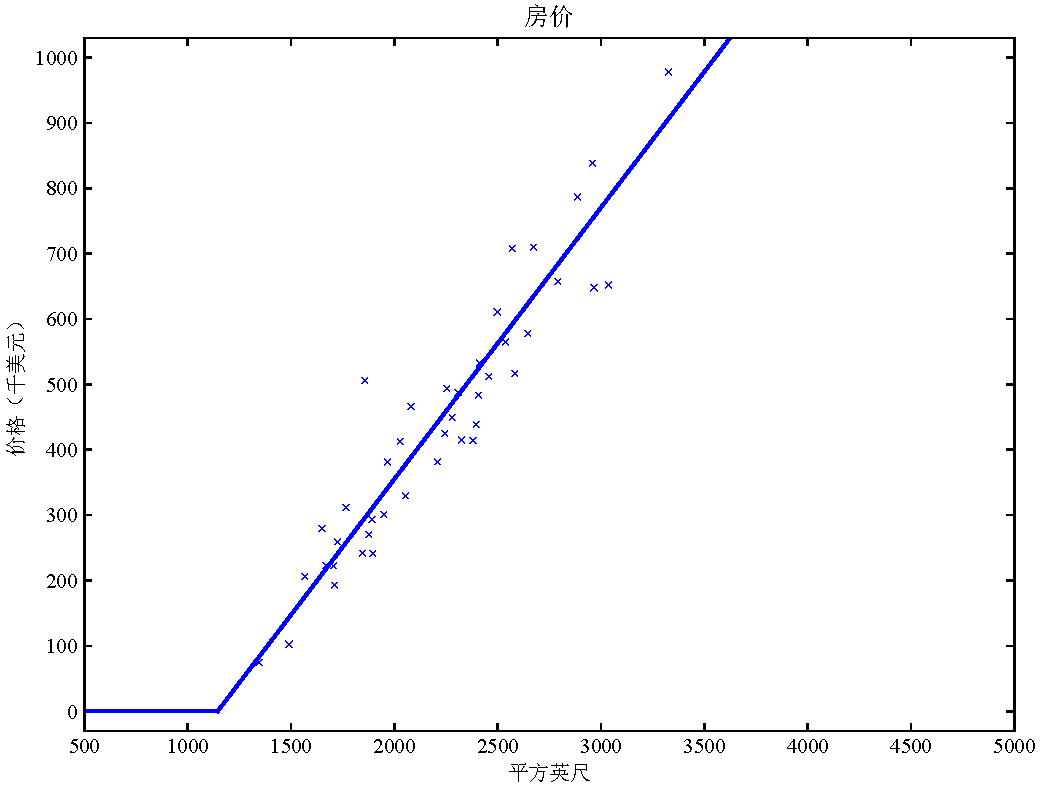
\includegraphics[width=0.5\linewidth]{figs/house_dataset_relu.pdf}
    \caption{带拐点的房价拟合}
    \label{fig:7.1}
\end{figure}

项 $b$ 通常被称为“偏置”,向量 $w$ 被称为权重向量。这样的神经网络称之为 1 层。(后续将定义多层的含义。)

\subsection*{堆叠神经元}

更复杂的神经网络可以将上述单个神经元“堆叠”在一起,使得一个神经元的输出作为下一个神经元的输入,从而产生更复杂的函数。
现在来深化房价预测的例子。除了房屋大小,假设还知道卧室数量、邮政编码和社区财富。构建神经网络类似于乐高积木:将单个积木堆叠在一起以构建复杂的结构。 这同样适用于神经网络:将单个神经元堆叠在一起以创建复杂的神经网络。
给定这些特征 (大小、卧室数量、邮政编码和财富),可能会决定房屋价格取决于其可容纳的最大家庭人数。假设家庭人数是房屋大小和卧室数量的函数 (参见图 \ref{fig:7.2})。邮政编码可以提供额外信息,例如社区的步行便利程度 (即,是否可以步行到杂货店或需要开车)。结合邮政编码和社区财富可以预测当地小学的质量。可以认为,房屋价格最终取决于这三个特征。

\begin{figure}[H]
\centering
\begin{tikzpicture}
\tikzstyle{nnnode}=[circle,draw,minimum size=1.5em]
    \node (phi2) [nnnode] {};
    \node (phi1) [nnnode, above=4mm of phi2] {};
    \node (phi3) [nnnode, below=6mm of phi2] {};
    \node (size) [above left=0mm and 5mm of phi1, label=left:{大小}] {};
    \node (bedrooms) [below left=0mm and 5mm of phi1, label=left:{卧室数量}] {};
    \node (zipcode) [below left=1mm and 5mm of phi2, label=left:{邮政编码}] {};
    \node (wealth) [below left=0mm and 5mm of phi3, label=left:{财富}] {};

    \node (output) [nnnode, right=25mm of phi2, label=right:{价格 $y$}] {};

    \draw[->] (phi1) -- (output) node [sloped, midway, yshift=7pt, font=\scriptsize] {家庭人数};
    \draw[->] (phi2) -- (output) node [sloped, near start, yshift=-7pt, font=\scriptsize] {\quad 步行便利程度};
    \draw[->] (phi3) -- (output) node [sloped, midway, yshift=-7pt, font=\scriptsize] {学校质量};
    \draw[->] (size) -- (phi1);
    \draw[->] (bedrooms) -- (phi1);
    \draw[->] (zipcode) -- (phi2);
    \draw[->] (zipcode) -- (phi3);
    \draw[->] (wealth) -- (phi3);
\end{tikzpicture}
\caption{预测房屋价格的小型神经网络示意图}\label{fig:7.2}
\end{figure}

形式上,神经网络的输入是一组输入特征 $x_1, x_2, x_3, x_4$。将“家庭人数”、“步行便利程度”和“学校质量”的中间变量记为 $a_1, a_2, a_3$ (这些 $a_i$ 通常被称为“隐藏单元”或“隐藏神经元”)。将每个 $a_i$ 表示为以 $x_1, \dots, x_4$ 的子集为输入的单神经元神经网络。然后,如在图 \ref{fig:7.1} 中,将有以下参数化:
\begin{align*}
    a_1 &= \text{ReLU}(\theta_1 x_1 + \theta_2 x_2 + \theta_3) \\
    a_2 &= \text{ReLU}(\theta_4 x_3 + \theta_5) \\
    a_3 &= \text{ReLU}(\theta_6 x_3 + \theta_7 x_4 + \theta_8)
\end{align*}
其中 $(\theta_1, \dots, \theta_8)$ 是参数。现在将最终输出 $\bar{h}_\theta(x)$ 表示为以 $a_1, a_2, a_3$ 为输入的另一个线性函数,得到\footnote{通常,对于多层神经网络,在末端,靠近输出处,不会应用 ReLU,特别是当输出不一定是正数时。}
\begin{equation}
    \bar{h}_\theta(x) = \theta_9 a_1 + \theta_{10} a_2 + \theta_{11} a_3 + \theta_{12}
    \label{eq:7.13}
\end{equation}
其中 $\theta$ 包含所有参数 $(\theta_1, \dots, \theta_{12})$。

现在将输出表示为以参数 $\theta$ 为输入的相当复杂的函数 $x$。然后可以使用第 \ref{sec:7.1} 节中的机制来学习参数 $\theta$。

\subsection*{生物神经网络的启发}

顾名思义,人工神经网络受到生物神经网络的启发。隐藏单元 $a_1, \dots, a_m$ 对应于生物神经网络中的神经元,参数 $\theta_i$ 对应于突触。然而,现代深度人工神经网络与生物神经网络的相似程度尚不清楚。例如,也许没有多少神经科学家认为生物神经网络可以有 1000 层,而一些现代人工神经网络则不然 (将在后续中详细阐述层的概念)。此外,人类大脑更新神经网络的方式是否与计算机科学家学习人工神经网络的方式 (使用反向传播,将在下一节介绍) 相似,这是一个悬而未决的问题。

\subsection*{两层全连接神经网络}

通过利用关于“家庭人数”、“步行便利程度”和“学校质量”如何由输入决定的重要先验知识/信念,构建了公式 \eqref{eq:7.13} 中的神经网络。隐含地假设知道家庭人数是一个重要的数量,并且它只能由“大小”和“卧室数量”确定。这样的先验知识可能不适用于其他应用。更灵活和通用的方法是为中间变量 $a_i$ 编写一个通用的参数化,作为所有 $x_1, \dots, x_4$ 的函数:
\begin{align}
    a_1 &= \text{ReLU}(w_1^\top x + b_1), \text{其中}\  w_1 \in \mathbb{R}^4 \text{且}\  b_1 \in \mathbb{R} \label{eq:7.14}\\
    a_2 &= \text{ReLU}(w_2^\top x + b_2), \text{其中}\  w_2 \in \mathbb{R}^4 \text{且}\  b_2 \in \mathbb{R} \notag\\
    a_3 &= \text{ReLU}(w_3^\top x + b_3), \text{其中}\  w_3 \in \mathbb{R}^4 \text{且}\  b_3 \in \mathbb{R} \notag
\end{align}

仍然使用上面定义的 $a_1, a_2, a_3$ 来定义 $\bar{h}_\theta(x)$。这样就得到了一个所谓的\textbf{全连接神经网络 (fully-connected neural network)},因为所有中间变量 $a_i$ 都依赖于所有输入 $x_i$。

为了通用性,具有 $m$ 个隐藏单元和 $d$ 维输入 $x \in \mathbb{R}^d$ 的两层全连接神经网络定义为
\begin{align}
    \forall j \in \{1, \dots, m\}, \quad z_j &= w_j^{[1]^\top} x + b_j^{[1]} \ \text{其中}\  w_j^{[1]} \in \mathbb{R}^d, b_j^{[1]} \in \mathbb{R} 
    \label{eq:7.15}\\
    a_j &= \text{ReLU}(z_j), \notag \\
    a &= [a_1, \dots, a_m]^\top \in \mathbb{R}^m \notag \\
    \bar{h}_\theta(x) &= w^{[2]^\top} a + b^{[2]} \text{其中}\  w^{[2]} \in \mathbb{R}^m, b^{[2]} \in \mathbb{R}
    \label{eq:7.16}
\end{align}

请注意,默认情况下,$\mathbb{R}^d$ 中的向量被视为列向量,特别是 $a$ 是一个分量为 $a_1, a_2, \dots, a_m$ 的列向量。索引 $^{[1]}$ 和 $^{[2]}$ 用于区分两组参数:$w_j^{[1]}$ (每个都是 $\mathbb{R}^d$ 中的向量) 和 $w^{[2]}$ (它是 $\mathbb{R}^m$ 中的向量)。稍后将更详细地讨论这些。

\subsection*{向量化}

在引入具有更多层和更复杂结构的神经网络之前,将使用更多的矩阵和向量符号简化神经网络的表达式。向量化的另一个重要动机是实现中的速度。为了有效地实现神经网络,在使用循环时必须小心。在代码中实现公式 \eqref{eq:7.15} 的最自然方法可能是使用 for 循环。在实践中,当输入和隐藏单元的维度很高时,使用循环会导致代码运行非常慢。利用 GPU 的并行性对于深度学习的发展至关重要。

这催生了向量化。向量化不是使用循环,而是利用矩阵代数和高度优化的数值线性代数库 (例如 BLAS) 来快速运行神经网络计算。在深度学习时代之前,for 循环可能足以处理较小的数据集,但现代深度网络和最先进的数据集使用 for 循环将不可行。

将下面的两层全连接神经网络向量化。将权重矩阵 $W^{[1]} \in \mathbb{R}^{m \times d}$ 定义为所有向量 $w_j^{[1]}$ 的串联,如下所示:
\begin{equation}
    W^{[1]} = \begin{bmatrix}
    & - w_1^{[1]^\top} - & \\
    & - w_2^{[1]^\top} - & \\
    & \vdots & \\
    & - w_m^{[1]^\top} - &
    \end{bmatrix} \in \mathbb{R}^{m \times d}
    \label{eq:7.17}
\end{equation}

现在根据矩阵向量乘法的定义,可以将 $z = [z_1, \dots, z_m]^\top \in \mathbb{R}^m$ 写为
\begin{equation}
    \underbrace{\begin{bmatrix}
    & z_1 & \\
    & \vdots & \\
    & z_m &
    \end{bmatrix}}_{z \in \mathbb{R}^{m \times 1}} = \underbrace{\begin{bmatrix}
    & - w_1^{[1]^\top} - & \\
    & - w_2^{[1]^\top} - & \\
    & \vdots & \\
    & - w_m^{[1]^\top} - &
    \end{bmatrix}}_{W^{[1]} \in \mathbb{R}^{m \times d}} \underbrace{\begin{bmatrix}
    & x_1 & \\
    & x_2 & \\
    & \vdots & \\
    & x_d &
    \end{bmatrix}}_{x \in \mathbb{R}^{d \times 1}} + \underbrace{\begin{bmatrix}
    & b_1^{[1]} & \\
    & b_2^{[1]} & \\
    & \vdots & \\
    & b_m^{[1]} &
    \end{bmatrix}}_{b^{[1]} \in \mathbb{R}^{m \times 1}}
    \label{eq:7.18}
\end{equation}
或者简明地写成
\begin{equation}
    z = W^{[1]} x + b^{[1]}
    \label{eq:7.19}
\end{equation}
再次强调,在本书中,根据先前建立的约定,$\mathbb{R}^d$ 中的向量自动视为列向量,并且可以看作是一个 $d \times 1$ 维矩阵。(注意,这与 numpy 不同,在 numpy 中,向量在广播中被视为行向量。)

根据 $z \in \mathbb{R}^m$ 计算激活 $a \in \mathbb{R}^m$ 涉及 ReLU 函数的逐元素应用,这可以高效地并行计算。重载 ReLU 以进行逐元素应用 (也就是说,对于向量 $t \in \mathbb{R}^d$,ReLU($t$) 是一个向量,使得 $\text{ReLU}(t)_i = \text{ReLU}(t_i)$),所以,我们有
\begin{equation}
    a = \text{ReLU}(z)
    \label{eq:7.20}
\end{equation}

类似地定义 $W^{[2]} = [w^{[2]}]^\top \in \mathbb{R}^{1 \times m}$。那么,公式 \eqref{eq:7.16} 中的模型可以概括为
\begin{align}
    a &= \text{ReLU}(W^{[1]} x + b^{[1]}) \notag \\
    \bar{h}_\theta(x) &= W^{[2]} a + b^{[2]}
    \label{eq:7.21}
\end{align}
其中 $\theta$ 由 $W^{[1]}, W^{[2]}$ (通常称为权重矩阵) 和 $b^{[1]}, b^{[2]}$ (称为偏置) 组成。$W^{[1]}, b^{[1]}$ 的集合称为第一层,$W^{[2]}, b^{[2]}$ 称为第二层。激活 $a$ 称为隐藏层。两层神经网络也称为单隐藏层神经网络。

\subsection*{多层全连接神经网络}

有了这种简洁的表示法,就可以堆叠更多层以获得更深的全连接神经网络。令 $r$ 为层数 (权重矩阵数)。令 $W^{[1]}, \dots, W^{[r]}, b^{[1]}, \dots, b^{[r]}$ 为所有层的权重矩阵和偏置。那么多层神经网络可以写成
\begin{align}
    a^{[1]} &= \text{ReLU}(W^{[1]} x + b^{[1]}) \notag\\
    a^{[2]} &= \text{ReLU}(W^{[2]} a^{[1]} + b^{[2]}) \notag\\
    \dots \notag\\
    a^{[r-1]} &= \text{ReLU}(W^{[r-1]} a^{[r-2]} + b^{[r-1]}) \notag\\
    \bar{h}_\theta(x) &= W^{[r]} a^{[r-1]} + b^{[r]}
    \label{eq:7.22}
\end{align}

注意到,为了使上述方程有意义,权重矩阵和偏置需要具有兼容的维度。如果 $a^{[k]}$ 的维度为 $m_k$,则权重矩阵 $W^{[k]}$ 的维度应为 $m_k \times m_{k-1}$,偏置 $b^{[k]} \in \mathbb{R}^{m_k}$。此外,$W^{[1]} \in \mathbb{R}^{m_1 \times d}$ 且 $W^{[r]} \in \mathbb{R}^{1 \times m_{r-1}}$。

网络中的神经元总数为 $m_1 + \dots + m_r$,该网络中的参数总数为 $(d+1)m_1 + (m_1+1)m_2 + \dots + (m_{r-1}+1)m_r$。

有时为了符号一致性,也记 $a^{[0]} = x$ 且 $a^{[r]} = \bar{h}_\theta(x)$。那么有简单的递归关系
\begin{equation}
    a^{[k]} = \text{ReLU}(W^{[k]} a^{[k-1]} + b^{[k]}), \forall k = 1, \dots, r-1
    \label{eq:7.23}
\end{equation}
注意,如果在公式 \eqref{eq:7.22} 中有一个额外的 ReLU,则对于 $k=r$ 这也成立,但人们通常喜欢使最后一层为线性层 (即没有 ReLU),这样可以得到负输出,并且更容易将最后一层解释为线性模型。(关于可解释性的更多内容请参见本节的“与核方法的联系”段落。)

\subsection*{其他激活函数}

激活函数 ReLU 可以被许多其他将 $\mathbb{R}$ 映射到 $\mathbb{R}$ 的非线性函数 $\sigma(\cdot)$ 替换,例如
\begin{align}
    \sigma(z) &= \frac{1}{1 + e^{-z}} \quad (\text{sigmoid}) \label{eq:7.24} \\
    \sigma(z) &= \frac{e^z - e^{-z}}{e^z + e^{-z}} \quad (\text{tanh}) \label{eq:7.25} \\
    \sigma(z) &= \max\{z, \gamma z\}, \gamma \in (0, 1) \quad (\text{leaky ReLU}) \label{eq:7.26} \\
    \sigma(z) &= \frac{z}{2} \left[1 + \text{erf}\left(\frac{z}{\sqrt{2}}\right)\right] \quad (\text{GELU}) \label{eq:7.27} \\
    \sigma(z) &= \frac{1}{\beta} \log(1 + \exp(\beta z)), \beta > 0 \quad (\text{Softplus}) \label{eq:7.28}
\end{align}

\begin{figure}[H]
    \centering
    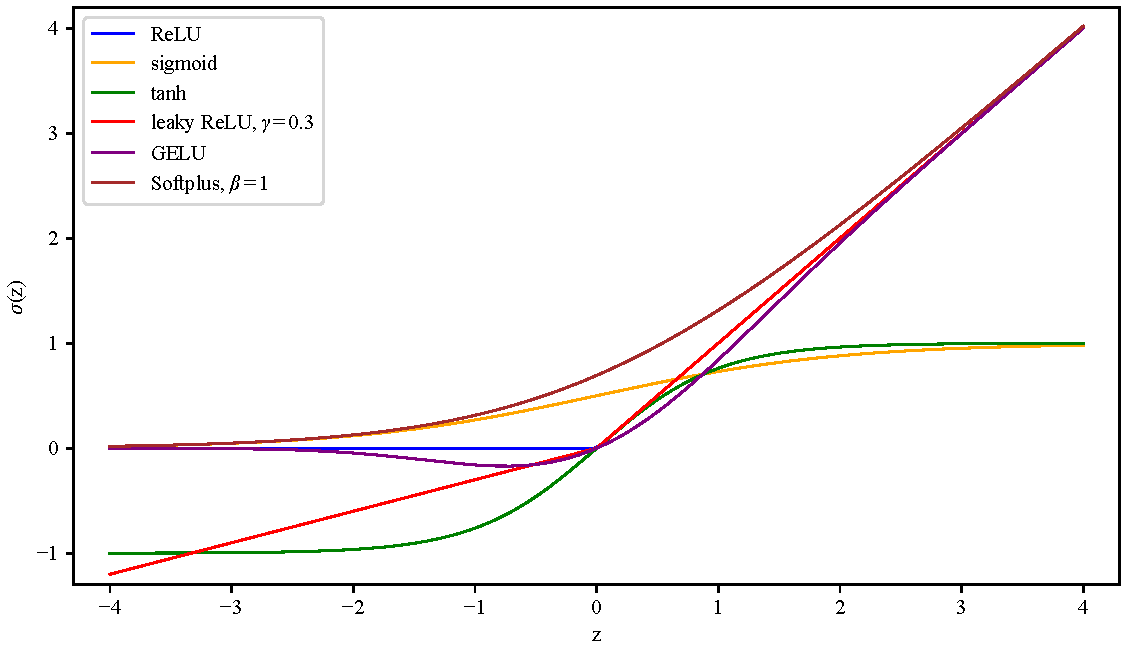
\includegraphics[width=0.8\linewidth]{figs/activations.pdf}
    \caption{深度学习中的激活函数}
    \label{fig:7.3}
\end{figure}

激活函数在图 \ref{fig:7.3} 中绘制。Sigmoid 和 tanh 现在使用得越来越少,部分原因是它们在两侧都有界,并且当 $z$ 趋于正负无穷时,它们的梯度会消失 (而所有其他激活函数在输入趋于正无穷时仍然有梯度)。Softplus 可以看作是 ReLU 的平滑版本,它具有适当的二阶导数,不过在实践中也不常用。GELU 和 leaky ReLU 都是 ReLU 的变体,但即使输入为负,它们也具有非零梯度。GELU (或其变体) 用于 NLP 模型,例如 BERT 和 GPT (这将在第 14 章讨论)。

\subsection*{为什么不使用恒等函数作为 $\sigma(z)$ ?} 

也即,为什么不使用 $\sigma(z) = z$?为了论证方便,假设 $b^{[1]}$ 和 $b^{[2]}$ 都为零。
假设 $\sigma(z) = z$,那么对于两层神经网络,有
\begin{align}
    \bar{h}_\theta(x) &= W^{[2]} a^{[1]} \label{eq:7.29} \\
    &= W^{[2]} \sigma(z^{[1]}) & \text{根据定义} \label{eq:7.30} \\
    &= W^{[2]} z^{[1]} & \text{因为}\  \sigma(z) = z \label{eq:7.31} \\
    &= W^{[2]} W^{[1]} x & \text{根据公式 \eqref{eq:7.18}} \label{eq:7.32} \\
    &= \tilde{W} x & \text{其中}\  \tilde{W} = W^{[2]} W^{[1]} \label{eq:7.33}
\end{align}
注意 $W^{[2]} W^{[1]}$ 如何合并成 $\tilde{W}$。

这是因为将一个线性函数应用于另一个线性函数会得到一个关于原始输入的线性函数 (即,可以构造一个 $\tilde{W}$ 使得 $\tilde{W} x = W^{[2]} W^{[1]} x$)。这会损失神经网络的许多表达能力,因为通常要预测的输出与输入之间存在非线性关系。如果没有非线性激活函数,神经网络将只会进行简单的线性回归。

\subsection*{与核方法的联系}

在之前的课程中,讨论了特征映射的概念。回忆一下,特征映射的主要动机是通过 $\theta^\top \phi(x)$ 来表示输入 $x$ 的非线性函数,其中 $\theta$ 是参数,$\phi(x)$ 是特征映射,是一个手工设计的关于原始输入 $x$ 的非线性函数。学习算法的性能很大程度上取决于特征映射 $\phi(x)$ 的选择。通常人们会利用领域知识来设计特征映射 $\phi(x)$ 以便适合特定的应用。选择特征映射的过程通常被称为\textbf{特征工程 (feature engineering)}。

可以将深度学习看作是一种自动学习正确特征映射(有时也称为“表示”)的方法,如下所示。假设用 $\beta$ 表示全连接神经网络(除了最后一层)的参数集合(公式 \eqref{eq:7.22})。然后可以将 $a^{[r-1]}$ 抽象为输入 $x$ 和参数 $\beta$ 的函数:$\beta: a^{[r-1]} = \phi_\beta(x)$。现在可以将模型写成
\begin{equation}
    \bar{h}_\theta(x) = W^{[r]} \phi_\beta(x) + b^{[r]} \label{eq:7.34}
\end{equation}
当 $\beta$ 固定时,$\phi_\beta(\cdot)$ 可以看作是特征映射,因此 $\bar{h}_\theta(x)$ 是关于特征 $\phi_\beta(x)$ 的线性模型。然而,训练神经网络时,参数 $\beta$ 和参数 $W^{[r]}, b^{[r]}$ 都会被优化,因此我们不仅在特征空间中学习线性模型,还在学习一个好的特征映射 $\phi_\beta(\cdot)$ 本身,以便在特征映射之上使用线性模型能够准确地进行预测。因此,深度学习倾向于较少依赖特定应用的领域知识,并且通常需要较少的特征工程。倒数第二层 $a^{[r]}$ 通常被(非正式地)称为深度学习背景下的学习特征或表示。

在房价预测的例子中,全连接神经网络不需要指定中间量,例如“家庭规模”,并且可以自动发现倒数第二层(即激活 $a^{[r-1]}$)中的一些有用特征,并使用它们来线性预测房价。从一个数据集获得的特征映射或表示(即函数 $\phi_\beta(\cdot)$)也可以用于其他数据集,这表明它们包含关于数据的基本信息。然而,通常神经网络会发现复杂的特征,这些特征对于预测输出非常有用,但对于人类来说可能难以理解或解释。这就是为什么有些人将神经网络称为\textit{黑箱 (black box)},因为很难理解它发现的特征。

\section{现代神经网络的模块}\label{sec:7.3}

第 \ref{sec:7.2} 节公式 \eqref{eq:7.22} 中介绍的多层神经网络现在通常被称为多层感知机 (MLP)。现代神经网络在实践中通常更复杂,由多个构建块或多层构建块组成。在本节中,将介绍一些其他的构建块并讨论可能的组合方式。

首先,每个矩阵乘法可以看作是一个构建块。考虑一个带有参数 $(W, b)$ 的矩阵乘法运算,其中 $W$ 是权重矩阵,$b$ 是偏置向量,作用于输入 $z$,
\begin{equation}
    \text{MM}_{W,b}(z) = W z + b. \label{eq:7.35}
\end{equation}
注意,这里隐含地假设所有维度都兼容。当在上下文中清晰或对讨论不重要时,也会省略 MM 的下标用以简化。

然后,MLP 可以写成多个矩阵乘法模块和非线性激活模块(也可以看作是构建块)的组合:
\begin{equation}
    \text{MLP}(x) = \text{MM}_{W^{[r]}, b^{[r]}} (\sigma(\text{MM}_{W^{[r-1]}, b^{[r-1]}} (\sigma(\cdots \text{MM}_{W^{[1]}, b^{[1]}}(x))))). \label{eq:7.36}
\end{equation}
或者,当省略表示参数的下标时,可以写成
\begin{equation}
    \text{MLP}(x) = \text{MM}(\sigma(\text{MM}(\sigma(\cdots \text{MM}(x))))). \label{eq:7.37}
\end{equation}
注意,在本讲义中,默认情况下,所有模块都有不同的参数集,并且参数的维度是有意义的。

较大的模块也可以通过较小的模块定义,例如,一个激活层 $\sigma$ 和一个矩阵乘法层 MM 经常组合在一起,在许多论文中被称为“层”。人们通常通过在图中指示这些模块之间的依赖关系来绘制架构。例如,参见图 \ref{fig:7.4} 左侧的 MLP 示意图。

\subsection*{残差连接}

一种非常有影响力的用于视觉应用的神经网络架构是 ResNet,它使用了残差连接,这些连接现在几乎用于所有大规模深度学习架构中。使用上面介绍的符号,一个非常简化的残差块可以定义为
\begin{equation}
    \text{Res}(z) = z + \sigma(\text{MM}(\sigma(\text{MM}(z)))). \label{eq:7.38}
\end{equation}
一个简化版 ResNet 是许多残差块的组合,后接一个矩阵乘法,
\begin{equation}
    \text{ResNet-S}(x) = \text{MM}(\text{Res}(\text{Res}(\cdots \text{Res}(x)))). \label{eq:7.39}
\end{equation}
这些模块的依赖关系也绘制在图 \ref{fig:7.4} 右侧。

\begin{figure}[H]
    \centering
    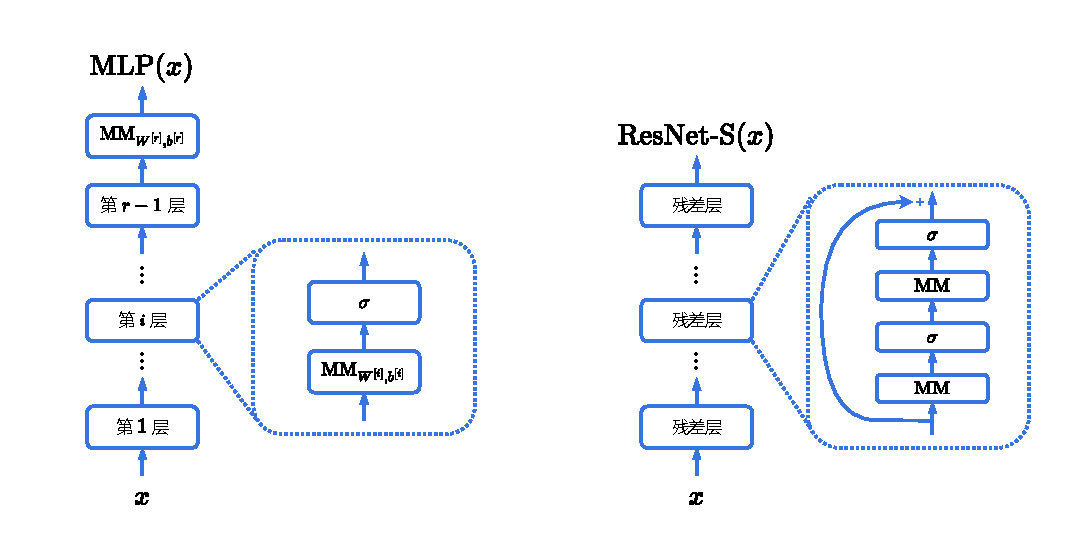
\includegraphics[width=1.0\linewidth]{figs/nn_architecture.pdf}
    \caption{网络架构示意图。\textbf{左图:} $r$ 层的MLP。\textbf{右图:} 残差网络。}
    \label{fig:7.4}
\end{figure}

注意,ResNet-S 与经典论文 [\cite{he2016resnet}] 中介绍的 ResNet 架构仍不完全相同,因为 ResNet 使用卷积层而不是普通的矩阵乘法,并在卷积和激活之间添加了批量归一化。下面将介绍卷积层和批量归一化的一些变体。ResNet-S 和层归一化是 Transformer 架构的一部分,它们在现代大型语言模型中被广泛使用。

\subsection*{层归一化}

层归一化,本文中记为 LN,是一个将向量 $z \in \mathbb{R}^m$ 映射到规范化的向量 $\text{LN}(z) \in \mathbb{R}^m$ 的模块。它通常在非线性激活之后使用。

首先定义层归一化的一个子模块,记为 LN-S。
\begin{equation}
    \text{LN-S}(z) = \begin{bmatrix}
        &\frac{z_1 - \hat{\mu}}{\hat{\sigma}}& \\
        &\frac{z_2 - \hat{\mu}}{\hat{\sigma}}& \\
        &\vdots& \\
        &\frac{z_m - \hat{\mu}}{\hat{\sigma}}&
    \end{bmatrix}, \label{eq:7.40}
\end{equation}
其中 $\hat{\mu} = \frac{\sum_{i=1}^m z_i}{m}$ 是向量 $z$ 的实际均值,$\hat{\sigma} = \sqrt{\frac{\sum_{i=1}^m (z_i - \hat{\mu})^2}{m}}$ 是 $z$ 中元素的实际标准差\footnote{注意,这里的实际标准差是除以 $m$ 而不是 $m-1$,因为所感兴趣的是使 $\text{LN-S}(z)$ 的输出的平方和等于 1(与统计学中估计标准差不同)。}。直观上看,LN-S$(z)$ 是一个经过归一化处理的向量,其实际均值为零,实际标准差为 1。

通常零均值和标准差 1 并非最理想的归一化方案,因此层归一化引入了可学习的标量参数 $\beta$ 和 $\gamma$ 作为期望的均值和标准差,并使用仿射变换将 LN-S$(z)$ 的输出转换为均值为 $\beta$、标准差为 $\gamma$ 的向量。
\begin{equation}
    \text{LN}(z) = \beta + \gamma \cdot \text{LN-S}(z) = \begin{bmatrix}
        &\beta + \gamma \left(\frac{z_1 - \hat{\mu}}{\hat{\sigma}}\right)& \\
        &\beta + \gamma \left(\frac{z_2 - \hat{\mu}}{\hat{\sigma}}\right)& \\
        &\vdots& \\
        &\beta + \gamma \left(\frac{z_m - \hat{\mu}}{\hat{\sigma}}\right)&
    \end{bmatrix}. \label{eq:7.41}
\end{equation}
这里,第一个 $\beta$ 技术上应该解释为一个所有元素都是标量 $\beta$ 的向量。还需要注意,$\hat{\mu}$ 和 $\hat{\sigma}$ 也是 $z$ 的函数,在计算层归一化的导数时不应将其视为常数。此外,$\beta$ 和 $\gamma$ 是可学习参数,因此层归一化是一个带参数的模块(与不带任何参数的激活层不同)。

\vspace{0.5em}
\noindent\textit{尺度不变性:}层归一化一个重要的性质是它使得模型对参数的缩放具有不变性,具体如下。假设考虑将 LN 与 $\text{MM}_{W,b}(z)$ 组合,得到一个子网络 $\text{LN}(\text{MM}_{W,b}(z))$。那么,当 $\text{MM}_{W,b}$ 中的参数被缩放时,这个子网络的输出不会改变:
\begin{equation}
    \text{LN}(\text{MM}_{\alpha W, \alpha b}(z)) = \text{LN}(\text{MM}_{W,b}(z)), \forall \alpha > 0. \label{eq:7.42}
\end{equation}
为了说明这一点,首先知道 LN-S$(\cdot)$ 是尺度不变的:
\begin{equation}
    \text{LN-S}(\alpha z) = \begin{bmatrix}
        &\frac{\alpha z_1 - \alpha \hat{\mu}}{\alpha \hat{\sigma}}& \\
        &\frac{\alpha z_2 - \alpha \hat{\mu}}{\alpha \hat{\sigma}}& \\
        &\vdots& \\
        &\frac{\alpha z_m - \alpha \hat{\mu}}{\alpha \hat{\sigma}}&
    \end{bmatrix} = \begin{bmatrix}
        &\frac{z_1 - \hat{\mu}}{\hat{\sigma}}& \\
        &\frac{z_2 - \hat{\mu}}{\hat{\sigma}}& \\
        &\vdots& \\
        &\frac{z_m - \hat{\mu}}{\hat{\sigma}}&
    \end{bmatrix} = \text{LN-S}(z). \label{eq:7.43}
\end{equation}
然后有
\begin{align}
    \text{LN}(\text{MM}_{\alpha W, \alpha b}(z)) &= \beta + \gamma \text{LN-S}(\text{MM}_{\alpha W, \alpha b}(z)) \label{eq:7.44} \\
    &= \beta + \gamma \text{LN-S}(\alpha \text{MM}_{W,b}(z)) \label{eq:7.45} \\
    &= \beta + \gamma \text{LN-S}(\text{MM}_{W,b}(z)) \label{eq:7.46} \\
    &= \text{LN}(\text{MM}_{W,b}(z)). \label{eq:7.47}
\end{align}

由于这一性质,大多数用于大规模计算机视觉和语言应用的现代深度学习架构都具有以下尺度不变性,即对于除最后一层权重 $W_{\text{last}}$ 以外的所有权重 $W$,网络 $f$ 具有 $f_{W_{\text{last}}, \alpha W}(x) = f_{W_{\text{last}}, W}(x)$ 对于任意 $\alpha > 0$ 成立。这里,最后一层的权重是特殊的,因为在最后一层权重之后通常没有层归一化或批量归一化。

\vspace{0.5em}
\noindent\textit{其他归一化层:}还有几种其他归一化层,旨在将神经网络的中间层归一化到更固定和可控的尺度,例如批量归一化 [?] 和组归一化 [?]。批量归一化和组归一化更常用于计算机视觉应用,而层归一化更常用于语言应用。

\subsection*{卷积层}

卷积神经网络是由卷积层(以及许多其他模块)组成的神经网络,特别适用于计算机视觉应用。为了简化说明,本文重点介绍 1-D 卷积,并在本小节末尾非正式地简要提及 2-D 卷积。(2-D 卷积更适合于具有两个维度的图像。1-D 卷积也用于自然语言处理。)

首先介绍一个简化版本的 1-D 卷积层,记为 Conv1D-S$(\cdot)$,它是一种具有特殊结构的矩阵乘法层。Conv1D-S 的参数是一个滤波器向量 $w \in \mathbb{R}^k$,其中 $k$ 称为滤波器大小(通常 $k \ll m$),以及一个标量偏置 $b$。滤波器有时也称为核(但与核方法中的核无关)。为简单起见,假设 $k = 2\ell + 1$ 是一个奇数。首先在输入向量 $z$ 的两端填充零,即 $z_{1-\ell} = z_{1-\ell+1} = \cdots = z_0 = 0$ 和 $z_{m+1} = z_{m+2} = \cdots = z_{m+\ell} = 0$,并将 $z$ 看作一个 $(m+2\ell)$ 维向量。Conv1D-S 输出一个维度为 $\mathbb{R}^m$ 的向量,其中每个输出维度是 $z$ 中子集元素的线性组合,系数来自 $w$,
\begin{equation}
    \text{Conv1D-S}(z)_i = w_1 z_{i-\ell} + w_2 z_{i-\ell+1} + \cdots + w_{2\ell+1} z_{i+\ell} = \sum_{j=1}^{2\ell+1} w_j z_{i-\ell+(j-1)}. \label{eq:7.48}
\end{equation}
因此,可以将 Conv1D-S 视为具有共享参数的矩阵乘法:$\text{Conv1D-S}(z) = Qz$,其中
\begin{equation}
    Q = \begin{bmatrix}
        &w_{\ell+1} &\cdots &w_{2\ell+1} & &\\
        &\vdots     &\ddots &\ddots      &w_{2\ell+1} & &\\
        &w_1        &\ddots &\ddots      &\ddots &\ddots & &\\
        &           &w_1    &\ddots      &\ddots &\ddots &w_{2\ell+1} &\\
        &           &       &\ddots      &\ddots &\ddots &\vdots &\\
        &           &       &            &w_1    &\cdots &w_{\ell+1} &
        
    \end{bmatrix}. \label{eq:7.49}
\end{equation}
注意,$Q_{i,j} = Q_{i-1,j-1}$ 对于所有 $i, j \in \{2, \ldots, m\}$ 都成立,因此卷积是一种带有参数共享的矩阵乘法。还注意到,计算卷积只需要 $O(km)$ 的时间,而计算一般的矩阵乘法需要 $O(m^2)$ 的时间。卷积有 $k$ 个参数,而一般的矩阵乘法有 $m^2$ 个参数。因此,卷积应该比一般的矩阵乘法效率高得多(只要施加的附加结构不损害模型的灵活性以适应数据)。

还注意到,在实践中存在许多卷积层的变体,与这里定义的有所不同,例如,填充零的方式或有时卷积层输出的维度可能与输入的维度不同。为了简化,这里省略了一些这些细节。

实践中使用的卷积层也有许多“通道”,上面的简化版本对应于 1 通道版本。形式上,Conv1D 接受 $C$ 个向量 $z_1, \ldots, z_C \in \mathbb{R}^m$ 作为输入,其中 $C$ 称为通道数。换句话说,更一般的版本 Conv1D 接受一个矩阵作为输入,它是 $z_1, \ldots, z_C$ 的拼接,维度为 $m \times C$。它可以输出 $C'$ 个维度为 $m$ 的向量,记为 $\text{Conv1D}(z)_1, \ldots, \text{Conv1D}(z)_{C'}$,其中 $C'$ 称为输出通道,或等效地一个维度为 $m \times C'$ 的矩阵。每个输出是应用于不同通道的简化卷积之和。
\begin{equation}
    \forall i \in [C'], \text{Conv1D}(z)_i = \sum_{j=1}^C \text{Conv1D-S}_{i,j}(z_j). \label{eq:7.50}
\end{equation}
注意,每个 $\text{Conv1D-S}_{i,j}$ 都是具有不同参数的模块,因此总参数数量是 $k \times C \times C'$(Conv1D-S 的参数数量 $\times$ Conv1D-S$_{i,j}$ 的数量)$= kCC'$。相比之下,从 $\mathbb{R}^{m \times C}$ 到 $\mathbb{R}^{m \times C'}$ 的一般线性映射具有 $m^2CC'$ 个参数。卷积的参数也可以表示为维度为 $k \times C \times C'$ 的三维张量。

\vspace{0.5em}
\noindent\textit{2-D 卷积(简述):}单通道的 2-D 卷积,记为 Conv2D-S,类似于 Conv1D-S,但接受一个 2 维输入 $z \in \mathbb{R}^{m \times m}$ 并应用一个 $k \times k$ 大小的滤波器,输出 Conv2D-S$(z) \in \mathbb{R}^{m \times m}$。完整的 2-D 卷积层,记为 Conv2D,接受一系列矩阵 $z_1, \ldots, z_C \in \mathbb{R}^{m \times m}$ 作为输入,或者等效地一个 3-D 张量 $z = (z_1, \ldots, z_C) \in \mathbb{R}^{m \times m \times C}$,并输出一系列矩阵 $\text{Conv2D}(z)_1, \ldots, \text{Conv2D}(z)_{C'} \in \mathbb{R}^{m \times m}$,也可以看作一个维度为 $\mathbb{R}^{m \times m \times C'}$ 的 3D 张量。每个输出通道是应用于所有输入通道的 Conv2D-S 层结果的总和。
\begin{equation}
    \forall i \in [C'], \text{Conv2D}(z)_i = \sum_{j=1}^C \text{Conv2D-S}_{i,j}(z_j). \label{eq:7.51}
\end{equation}
因为有 $CC'$ 个 Conv2D-S 模块,并且每个 Conv2D-S 模块有 $k^2$ 个参数,所以总参数数量是 $CC'k^2$。其参数也可以看作一个维度为 $C \times C' \times k \times k$ 的四维张量。

\section{反向传播}\label{sec:7.4}

本节将介绍反向传播,或称自动微分,它能高效地计算损失函数的梯度 $\nabla J(\theta)$。首先,从一个非正式定理开始,该定理指出,只要一个\textit{实值函数 (real-valued function)} $f$ 可以通过一个可微网络或电路高效地计算/评估,那么它的梯度也可以在相似的时间内高效地计算。然后,将展示如何在神经网络中具体实现这一点。

由于通用定理的严格性并非本节的主要重点,将使用非正式定义来介绍术语。可微电路或可微网络是指一系列可微算术运算 (加法、减法、乘法、除法等) 和基本可微函数 (ReLU、exp、log、sin、cos 等) 的组合。电路的大小定义为这些运算和基本函数的总数。假设每个运算和函数及其导数或偏导数都可以在 $O(1)$ 时间内计算。

\begin{theorem}\label{theorem:7.4.1}
    \textit{[反向传播,或称自动微分的非正式表述]} 
    
    \noindent 假设有一个大小为 $N$ 的可微电路计算一个实值函数 $f: \mathbb{R}^\ell \to \mathbb{R}$。那么,梯度 $\nabla f$ 可以通过一个大小为 $O(N)$ 的电路在 $O(N)$ 的时间内计算\footnote{注意到,如果函数 $f$ 的输出不依赖于某些输入的分量,则默认将关于这些分量的梯度设为零。在本节的计算方案中,将梯度设为零不计入总运行时间。因此,当 $N \le \ell$ 时,可以在 $O(N)$ 时间内计算梯度,这可能甚至小于 $\ell$。}。
\end{theorem}

注意到,对于第 $j$ 个样本的损失函数 $J^{(j)}(\theta)$ 可以通过包含加法、减法、乘法和非线性激活等运算和函数的序列计算。因此,定理表明,应该能够在与计算 $J^{(j)}(\theta)$ 本身相似的时间内计算 $\nabla J^{(j)}(\theta)$。这不仅适用于第 \ref{sec:7.2} 节介绍的全连接神经网络,也适用于许多其他使用更高级模块的神经网络。

注意到,自动微分或反向传播已经集成到所有深度学习库中,例如 tensorflow 和 pytorch,因此在实践中,大多数情况下研究人员无需编写自己的反向传播算法。然而,理解其原理对于深入理解深度学习的工作原理非常有帮助。

本节的其余部分组织如下。在第 \ref{sec:7.4.1} 节中,将从一个新的角度回顾基本链式法则,这对于理解反向传播特别有用。第 \ref{sec:7.4.2} 节将介绍反向传播的通用策略。第 \ref{sec:7.4.2} 节将讨论如何计算神经网络中使用的基本模块的所谓反向函数,第 \ref{sec:7.4.4} 节将把所有内容组合起来,得到一个用于 MLP 的具体反向传播算法。

\subsection{偏导数初步}\label{sec:7.4.1}

假设标量变量 $J$ 依赖于某些变量 $z$ (可以是标量、矩阵或高阶张量),记 $\frac{\partial J}{\partial z}$ 为 $J$ 关于变量 $z$ 的偏导数。这里的惯例是 $\frac{\partial J}{\partial z}$ 与 $z$ 本身具有完全相同的维度。例如,如果 $z \in \mathbb{R}^{m \times n}$,则 $\frac{\partial J}{\partial z} \in \mathbb{R}^{m \times n}$,并且 $\frac{\partial J}{\partial z}$ 的 $(i, j)$ 元素等于 $\frac{\partial J}{\partial z_{ij}}$。

\begin{remark}\label{remark:7.4.1}
    当 $J$ 和 $z$ 都不是标量时,$J$ 关于 $z$ 的偏导数变成矩阵或张量,并且符号变得有些棘手。除了处理数学或符号上的挑战之外,这些多元函数的偏导数不仅计算和存储成本高昂,而且实际上也很少显式构造这些偏导数。作者的经验表明,只考虑标量函数对向量、矩阵或张量的导数通常更有效。故在本讲义中,不会讨论多元函数的导数。
\end{remark} 

\subsubsection*{链式法则}

下面回顾微积分中的链式法则,但我们的视角和符号更侧重于自动微分。

考虑一个标量变量 $J$,它由函数 $f$ 和 $g$ 在某个变量 $z$ 上的复合得到,
\begin{align}
    z &\in \mathbb{R}^m \notag\\
    u &= g(z) \in \mathbb{R}^n \notag\\
    J &= f(u) \in \mathbb{R}. \label{eq:7.52}
\end{align}
下面的推导可以很容易地扩展到 $z$ 和 $u$ 是矩阵或张量的情况;但需要强调的是,最终变量 $J$ 是一个标量(参见备注 \ref{remark:7.4.1})。令 $u = (u_1, \dots, u_n)$,并令 $g(z) = \left(g_1(z), \dots, g_n(z)\right)$。那么,根据标准的链式法则,有
\begin{equation}
    \forall i \in \{1, \dots, m\}, \quad \frac{\partial J}{\partial z_i} = \sum_{j=1}^n \frac{\partial J}{\partial u_j} \cdot \frac{\partial g_j}{\partial z_i}. \label{eq:7.53}
\end{equation}
或者,当 $z$ 和 $u$ 都是向量时,采用向量化符号:
\begin{equation}
    \frac{\partial J}{\partial z} = \begin{bmatrix}
    &\frac{\partial g_1}{\partial z_1}&  &\cdots&  &\frac{\partial g_n}{\partial z_1}& \\
    &\vdots&  &\ddots&  &\vdots& \\
    &\frac{\partial g_1}{\partial z_m}&  &\cdots&  &\frac{\partial g_n}{\partial z_m}&
    \end{bmatrix} \cdot \frac{\partial J}{\partial u}. \label{eq:7.54}
\end{equation}
换句话说,反向函数总是从 $\frac{\partial J}{\partial u}$ 到 $\frac{\partial J}{\partial z}$ 的线性映射,但请注意,映射本身可以以复杂的方式依赖于 $z$。公式 \eqref{eq:7.54} 右侧的矩阵实际上是函数 $g$ 的雅可比矩阵的转置。然而,不会深入讨论雅可比矩阵的应用,以避免复杂性。部分原因在于,当 $z$ 是矩阵(或张量)时,要写出类似公式 \eqref{eq:7.54} 的形式,需要将 $z$ 展平为向量或引入张量-矩阵乘法的额外符号。从这个意义上说,公式 \eqref{eq:7.53} 在所有情况下都更方便有效。例如,当 $z \in \mathbb{R}^{r \times s}$ 是一个矩阵时,可以很容易地重写公式 \eqref{eq:7.53} 得到
\begin{equation}
    \forall i, k, \quad \frac{\partial J}{\partial z_{ik}} = \sum_{j=1}^n \frac{\partial J}{\partial u_j} \cdot \frac{\partial g_j}{\partial z_{ik}}, \label{eq:7.55}
\end{equation}
这将在第 \ref{sec:7.4.3} 节的一些推导中用到。

\vspace{0.5em}
\noindent\textit{链式法则的关键解释:}可以将上面的公式(公式 \eqref{eq:7.53} 或 \eqref{eq:7.54})看作是从 $\frac{\partial J}{\partial u}$ 计算 $\frac{\partial J}{\partial z}$ 的一种方法。考虑以下抽象问题:假设 $J$ 通过公式 \eqref{eq:7.52} 中定义的 $u$ 依赖于 $z$。然而,假设函数 $f$ 未知或函数 $f$ 很复杂,但已知 $\frac{\partial J}{\partial u}$ 的值。那么,公式 \eqref{eq:7.54} 提供了一种从 $\frac{\partial J}{\partial u}$ 计算 $\frac{\partial J}{\partial z}$ 的方法。
\begin{equation}
    \frac{\partial J}{\partial u} \quad \xRightarrow[\text{只需要关于}\  g(\cdot) \ \text{和}\  z \text{的信息}]{\text{利用链式法则和公式 \eqref{eq:7.54}} } \quad \frac{\partial J}{\partial z}. \label{eq:7.56}
\end{equation}
此外,此公式仅涉及关于 $g$ 的知识(更准确地说,$\frac{\partial g_j}{\partial z_i}$)。将反复利用这一点来处理 $g$ 是复杂网络 $f$ 的构建模块的情况。

根据经验,可以将公式 \eqref{eq:7.53} 或 \eqref{eq:7.54} 中的映射模块视为一个黑盒,并且定义一个数学符号也便于后续讨论\footnote{该函数也是 pytorch 中模块的 .backward() 方法。}。使用 $\mathcal{B}[g, z]$ 定义将 $\frac{\partial J}{\partial u}$ 映射到 $\frac{\partial J}{\partial z}$ 的函数,并记作
\begin{equation}
    \frac{\partial J}{\partial z} = \mathcal{B}[g, z]\left(\frac{\partial J}{\partial u}\right). \label{eq:7.57}
\end{equation}
称 $\mathcal{B}[g, z]$ 为模块 $g$ 的\textbf{反向函数 (backward function)}。注意,当 $z$ 固定时,$\mathcal{B}[g, z]$ 仅是从 $\mathbb{R}^n$ 到 $\mathbb{R}^m$ 的线性映射。使用公式 \eqref{eq:7.53},有
\begin{equation}
    (\mathcal{B}[g, z](v))_i = \sum_{j=1}^m \frac{\partial g_j}{\partial z_i} \cdot v_j. \label{eq:7.58}
\end{equation}
或者采用向量化符号,使用公式 \eqref{eq:7.54},有
\begin{equation}
    \mathcal{B}[g, z](v) = \begin{bmatrix}
    &\frac{\partial g_1}{\partial z_1}&  &\cdots&  &\frac{\partial g_n}{\partial z_1}& \\
    &\vdots&  &\ddots&  &\vdots& \\
    &\frac{\partial g_1}{\partial z_m}&  &\cdots&  &\frac{\partial g_n}{\partial z_m}&
    \end{bmatrix} \cdot v. \label{eq:7.59}
\end{equation}
因此 $\mathcal{B}[g, z]$ 可以看作一个矩阵。然而,实际上,$z$ 将不断变化,因此当 $g$ 固定时,反向映射必须针对不同的 $z$ 重新计算。因此,从经验上看,反向函数 $\mathcal{B}[g, z](v)$ 通常被视为一个函数,它接受 $z$($g$ 的输入)和 $v$($J$ 对某个变量的梯度,该变量被认为是 $g$ 的输出)作为输入,并输出一个向量,该向量被认为是 $J$ 对 $z$ 的梯度。

\subsection{反向传播的通用策略}\label{sec:7.4.2}

本节讨论自动微分的通用策略,以建立高层次的理解。然后,将把这种方法实例化到具体的神经网络中。采用的观点是,神经网络是由小的构建块组成的复杂组合,例如第 \ref{sec:7.3} 节中定义的 MM、$\sigma$、Conv2D、LN 等。注意,损失函数(例如,均方误差损失或交叉熵损失)也可以抽象地视为附加模块。因此,可以将损失函数 $J$(针对单个样本 $(x, y)$)抽象地写成许多模块的组合\footnote{严格来说,应该写成 $J = M_k(M_{k-1}(\cdots M_1(x)), y)$。然而,为了计算相对于参数的导数,将 $y$ 视为常数,因此为了符号的简洁性,可以将其视为 $M_k$ 的一部分。}:
\begin{equation}
    J = M_k(M_{k-1}(\cdots M_1(x))). \label{eq:7.60}
\end{equation}

例如,对于具有 MLP $\bar{h}_\theta(x)$(在公式 \eqref{eq:7.36} 和 \eqref{eq:7.37} 中定义)的二分类问题,损失函数可以写成公式 \eqref{eq:7.60} 的形式,其中 $M_1 = \text{MM}_{W^{[1]}, b^{[1]}}$,$M_2 = \sigma$, $M_3 = \text{MM}_{W^{[2]}, b^{[2]}}$,$\dots$,以及 $M_{k-1} = \text{MM}_{W^{[r]}, b^{[r]}}$, $M_k = \ell_{\text{logistic}}$。

从这个例子可以看出,有些模块涉及参数,而有些模块可能只涉及固定的操作集。为了通用性,假设每个 $M_i$ 都涉及一组参数 $\theta^{[i]}$,尽管当 $M_i$ 是像非线性激活这样的固定操作时,$\theta^{[i]}$ 可能是一个空集。之后将更详细地讨论模块化的粒度,但目前假设所有模块 $M_i$ 都足够简单。

引入用于公式 \eqref{eq:7.60} 中计算的中间变量:
\begin{align}
    u^{[0]} &= x \notag\\
    u^{[1]} &= M_1(u^{[0]}) \notag\\
    u^{[2]} &= M_2(u^{[1]}) \notag\\
    &\vdots \notag\\
    J = u^{[k]} &= M_k(u^{[k-1]}). \tag{F}\label{eq:F}
\end{align}

反向传播由两个过程组成:前向传播和反向传播。在前向传播中,算法根据定义 \eqref{eq:F} 按顺序计算 $u^{[1]}, \dots, u^{[k]}$,并将所有中间变量 $u^{[i]}$ 保存在内存中。

在反向传播中,首先按反向顺序计算 $J$ 对中间变量的导数,即 $\frac{\partial J}{\partial u^{[k]}}, \dots, \frac{\partial J}{\partial u^{[1]}}$,然后从 $\frac{\partial J}{\partial u^{[i]}}$ 和 $u^{[i-1]}$ 计算参数 $\theta^{[i]}$ 的导数 $\frac{\partial J}{\partial \theta^{[i]}}$。这两类计算可以相互交织,因为 $\frac{\partial J}{\partial \theta^{[i]}}$ 仅依赖于 $\frac{\partial J}{\partial u^{[i]}}$ 和 $u^{[i-1]}$,而不依赖于任何 $k < i$ 的 $\frac{\partial J}{\partial u^{[k]}}$。

首先通过引用第 \ref{sec:7.4.1} 节关于链式法则的讨论来理解为什么 $\frac{\partial J}{\partial u^{[i-1]}}$ 可以从 $\frac{\partial J}{\partial u^{[i]}}$ 和 $u^{[i-1]}$ 有效计算。通过设置 $u = u^{[i]}$ 和 $z = u^{[i-1]}$,以及 $f(u) = M_k(M_{k-1}(\cdots M_{i+1}(u)))$,以及 $g(\cdot) = M_i(\cdot)$,来实例化讨论。注意,$f$ 非常复杂,但不需要关于 $f$ 的任何具体信息。那么,结论性公式 \eqref{eq:7.56} 对应于
\begin{equation}
    \frac{\partial J}{\partial u^{[i]}} \quad \xRightarrow[\textbf{只需要关于}\  M_i(\cdot) \ \textbf{和}\  u^{[i-1]} \ \textbf{的信息}]{\text{链式法则}} \frac{\partial J}{\partial u^{[i-1]}}. \label{eq:7.61}
\end{equation}
更准确地说,根据公式 \eqref{eq:7.57},可以写成
\begin{align}
    \frac{\partial J}{\partial u^{[i-1]}} &= \mathcal{B}[M_i, u^{[i-1]}]\left(\frac{\partial J}{\partial u^{[i]}}\right). \tag{B1}\label{eq:B1}
\end{align}
将链式法则实例化为 $z = \theta^{[i]}$ 和 $u = u^{[i]}$,也有
\begin{align}
    \frac{\partial J}{\partial \theta^{[i]}} &= \mathcal{B}[M_i, \theta^{[i]}]\left(\frac{\partial J}{\partial u^{[i]}}\right). \tag{B2}\label{eq:B2}
\end{align}
有关算法的说明,请参见图 \ref{fig:7.5}。

\begin{figure}[H]
    \centering
    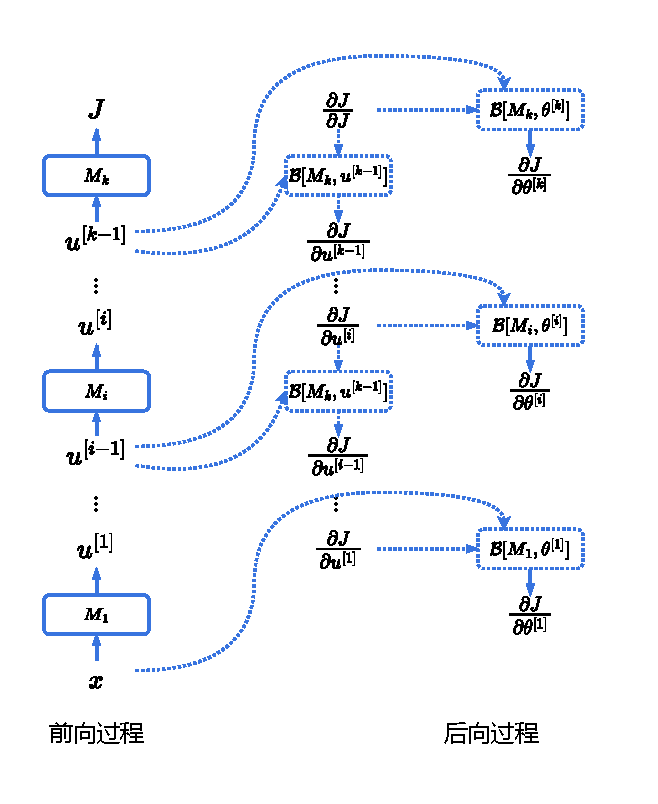
\includegraphics[width=0.7\linewidth]{figs/backpropagation.pdf}
    \caption{反向传播}
    \label{fig:7.5}
\end{figure}

\newpage
\begin{remark}\upshape
    \text{[计算效率和模块的粒度]} 
    
    \noindent 将复杂网络视为小型模块组合的主要根本目的是,小型模块往往具有可高效实现的后向函数。实际上,所有原子模块(如加法、乘法和 ReLU)的后向函数都可以像评估这些模块一样高效地计算(最多相差一个乘法常数因子)。利用这一事实,可以通过将神经网络视为许多原子操作的组合,并调用上面讨论的反向传播来证明定理 \ref{theorem:7.4.1}。然而,在实践中,会更常使用矩阵乘法、层归一化这类模块来模块化网络。正如后文所述,这些操作的后向函数的朴素实现也具有与这些函数的评估相同的运行时间。
\end{remark}


\subsection{基本模块的后向函数}\label{sec:7.4.3}

利用第 \ref{sec:7.4.2} 节的通用策略,只需计算网络中使用的所有模块 $M_i$ 的后向函数即可。本节计算基本模块 MM、激活函数 $\sigma$ 和损失函数的后向函数。

\vspace{0.5em}
\noindent\textit{MM 的后向函数:} 假设 $\text{MM}_{W,b}(z) = Wz + b$ 是一个矩阵乘法模块,其中 $z \in \mathbb{R}^m$ 且 $W \in \mathbb{R}^{n \times m}$。那么,对于 $v \in \mathbb{R}^n$,使用公式 \eqref{eq:7.59},有
\begin{equation}
    \mathcal{B}[\text{MM}, z](v) = \begin{bmatrix}
        &\frac{\partial (Wz+b)_1}{\partial z_1}& \cdots& \frac{\partial (Wz+b)_n}{\partial z_1}& \\
        &\vdots& \ddots& \vdots& \\
        &\frac{\partial (Wz+b)_1}{\partial z_m}& \cdots& \frac{\partial (Wz+b)_n}{\partial z_m}&
    \end{bmatrix} v. \label{eq:7.62}
\end{equation}
由于对于所有 $i \in [m], j \in [n]$,$\frac{\partial (Wz+b)_j}{\partial z_i} = \frac{\partial b_j + \sum_{k=1}^m W_{jk} z_k}{\partial z_i} = W_{ji}$,因此有
\begin{equation}
    \mathcal{B}[\text{MM}, z](v) = W^\top v \in \mathbb{R}^m. \label{eq:7.63}
\end{equation}
在上述推导中,将 MM 视为 $z$ 的函数。如果将 MM 视为 $W$ 和 $b$ 的函数,那么也可以计算参数变量 $W$ 和 $b$ 的后向函数。使用公式 \eqref{eq:7.59} 不太方便,因为变量 $W$ 是一个矩阵,而公式 \eqref{eq:7.59} 中的矩阵将是一个四阶张量,有书写难度。因此,使用 \eqref{eq:7.58}:
\begin{equation}
    (\mathcal{B}[\text{MM}, W](v))_{ij} = \sum_{k=1}^m \frac{\partial (Wz+b)_k}{\partial W_{ij}} \cdot v_k = \sum_{k=1}^m \frac{\partial \sum_{s=1}^m W_{ks} z_s}{\partial W_{ij}} \cdot v_k = v_i z_j. \label{eq:7.64}
\end{equation}
在向量化表示中,有
\begin{equation}
    \mathcal{B}[\text{MM}, W](v) = v z^\top \in \mathbb{R}^{n \times m}. \label{eq:7.65}
\end{equation}
对于变量 $b$,使用公式 \eqref{eq:7.59},有
\begin{equation}
    \mathcal{B}[\text{MM}, b](v) = \begin{bmatrix}
        &\frac{\partial (Wz+b)_1}{\partial b_1}& \cdots& \frac{\partial (Wz+b)_n}{\partial b_1}& \\
        &\vdots& \ddots& \vdots& \\
        &\frac{\partial (Wz+b)_1}{\partial b_n}& \cdots& \frac{\partial (Wz+b)_n}{\partial b_n}&
    \end{bmatrix} v = v. \label{eq:7.66}
\end{equation}
这里利用了当 $i \neq j$ 时 $\frac{\partial (Wz+b)_i}{\partial b_j} = 0$,当 $i = j$ 时 $\frac{\partial (Wz+b)_j}{\partial b_i} = 1$。

计算后向函数的计算效率是 $O(mn)$,与计算矩阵乘法结果的效率相同(相差一个常数因子)。

\vspace{0.5em}
\noindent\textit{激活函数的后向函数。} 假设 $M(z) = \sigma(z)$,其中 $\sigma$ 是一个逐元素的激活函数,且 $z \in \mathbb{R}^m$。那么,使用公式 \eqref{eq:7.59},有
\begin{align}
    \mathcal{B}[\sigma, z](v) &= \begin{bmatrix}
        &\frac{\partial \sigma(z_1)}{\partial z_1}& \cdots& \frac{\partial \sigma(z_m)}{\partial z_1}& \\
        &\vdots& \ddots& \vdots& \\
        &\frac{\partial \sigma(z_1)}{\partial z_m}& \cdots& \frac{\partial \sigma(z_m)}{\partial z_m}&
    \end{bmatrix} v \label{eq:7.67} \\
    &= \text{diag}(\sigma'(z_1), \dots, \sigma'(z_m))v \label{eq:7.68} \\
    &= \sigma'(z) \odot v \in \mathbb{R}^m. \label{eq:7.69}
\end{align}
这里利用了当 $j \neq i$ 时 $\frac{\partial \sigma(z_j)}{\partial z_i} = 0$,$\text{diag}(\lambda_1, \dots, \lambda_m)$ 表示对角线上为 $\lambda_1, \dots, \lambda_m$ 的对角矩阵,$\odot$ 表示两个同维度向量的逐元素乘积,$\sigma'(\cdot)$ 是激活函数 $\sigma$ 的导数(对向量逐元素应用)。关于计算效率,注意到乍一看,公式 \eqref{eq:7.67} 似乎表明后向函数需要 $O(m^2)$ 的时间,但公式 \eqref{eq:7.69} 表明它可以在 $O(m)$ 的时间内实现(这与评估函数的时间相同)。如果使用更小的模块,即把向量到向量的非线性激活视为 $m$ 个标量到标量的非线性激活,那么公式 \eqref{eq:7.67} 到 \eqref{eq:7.69} 的简化可能性不应感到惊讶,这时后向传播应该具有与前向传播相似的时间。

\vspace{0.5em}
\noindent\textit{损失函数的后向函数。} 当模块 $M$ 接受一个向量 $z$ 并输出一个标量时,根据公式 \eqref{eq:7.59},后向函数接受一个标量 $v$ 并输出一个向量,其分量为 $(\mathcal{B}[M, z](v))_i = \frac{\partial M}{\partial z_i} v$。因此,在向量化表示中,$\mathcal{B}[M, z](v) = \frac{\partial M}{\partial z} \cdot v$。

回想一下,平方损失 $\ell_{\text{MSE}}(z, y) = \frac{1}{2}(z-y)^2$。因此,$\mathcal{B}[\ell_{\text{MSE}}, z](v) = \frac{\partial \frac{1}{2}(z-y)^2}{\partial z} \cdot v = (z-y) \cdot v$。

对于逻辑损失,根据公式 \eqref{eq:2.6},有
\begin{equation}
    \mathcal{B}[\ell_{\text{logistic}}, t](v) = \frac{\partial \ell_{\text{logistic}}(t, y)}{\partial t} \cdot v = (1/(1 + \exp(-t)) - y) \cdot v. \label{eq:7.70}
\end{equation}

对于交叉熵损失,根据公式 \eqref{eq:2.17},有
\begin{equation}
    \mathcal{B}[\ell_{\text{ce}}, t](v) = \frac{\partial \ell_{\text{ce}}(t, y)}{\partial t} \cdot v = (\phi - e_y) \cdot v, \label{eq:7.71}
\end{equation}
其中 $\phi = \text{softmax}(t)$。

\subsection{MLP 的反向传播}\label{sec:7.4.4}

给定评估 MLP 损失所需的每个模块的后向函数,根据第 \ref{sec:7.4.2} 节的策略计算损失相对于隐藏激活和参数的梯度。
考虑一个具有逻辑损失的 $r$ 层 MLP。损失函数可以通过一系列操作计算(即前向传播),
\begin{align}
    z^{[1]} &= \text{MM}_{W^{[1]}, b^{[1]}}(x), \nonumber \\
    a^{[1]} &= \sigma(z^{[1]}), \nonumber \\
    z^{[2]} &= \text{MM}_{W^{[2]}, b^{[2]}}(a^{[1]}), \nonumber \\
    a^{[2]} &= \sigma(z^{[2]}), \nonumber \\
    &\vdots \nonumber \\
    z^{[r]} &= \text{MM}_{W^{[r]}, b^{[r]}}(a^{[r-1]}), \nonumber \\
    J &= \ell_{\text{logistic}}(z^{[r]}, y). \label{eq:7.72}
\end{align}
按后向顺序依次应用后向函数。首先,有
\begin{equation}
    \frac{\partial J}{\partial z^{[r]}} = \mathcal{B}[\ell_{\text{logistic}}, z^{[r]}]\left(\frac{\partial J}{\partial J}\right) = \mathcal{B}[\ell_{\text{logistic}}, z^{[r]}](1). \label{eq:7.73}
\end{equation}
然后,通过重复调用链式法则(公式 \eqref{eq:7.58}),迭代计算 $\frac{\partial J}{\partial a^{[i]}}$ 和 $\frac{\partial J}{\partial z^{[i]}}$:
\begin{align}
    \frac{\partial J}{\partial a^{[r-1]}} &= \mathcal{B}[\text{MM}, a^{[r-1]}]\left(\frac{\partial J}{\partial z^{[r]}}\right) \nonumber \\
    \frac{\partial J}{\partial z^{[r-1]}} &= \mathcal{B}[\sigma, z^{[r-1]}]\left(\frac{\partial J}{\partial a^{[r-1]}}\right) \nonumber \\
    &\vdots \nonumber \\
    \frac{\partial J}{\partial z^{[1]}} &= \mathcal{B}[\sigma, z^{[1]}]\left(\frac{\partial J}{\partial a^{[1]}}\right). \label{eq:7.74}
\end{align}
数值上,通过重复调用公式 \eqref{eq:7.69} 和 \eqref{eq:7.63},并选择不同的变量,计算这些量。
注意到中间值 $a^{[i]}$ 和 $z^{[i]}$ 在反向传播(公式 \eqref{eq:7.74})中使用,因此这些值需要在前向传播后存储在内存中。

接下来,通过调用公式 \eqref{eq:7.65} 和 \eqref{eq:7.66},计算参数的梯度:
\begin{equation}
    \begin{aligned}
        \frac{\partial J}{\partial W^{[r]}} &= \mathcal{B}[\text{MM}, W^{[r]}]\left(\frac{\partial J}{\partial z^{[r]}}\right) \\
        \frac{\partial J}{\partial b^{[r]}} &= \mathcal{B}[\text{MM}, b^{[r]}]\left(\frac{\partial J}{\partial z^{[r]}}\right) \\
        &\vdots \\
        \frac{\partial J}{\partial W^{[1]}} &= \mathcal{B}[\text{MM}, W^{[1]}]\left(\frac{\partial J}{\partial z^{[1]}}\right) \\
        \frac{\partial J}{\partial b^{[1]}} &= \mathcal{B}[\text{MM}, b^{[1]}]\left(\frac{\partial J}{\partial z^{[1]}}\right).
    \end{aligned} \label{eq:7.75}
\end{equation}

还注意到,公式 \eqref{eq:7.75} 中的计算块可以与公式 \eqref{eq:7.74} 中的计算块交织进行,因为一旦计算出 $\frac{\partial J}{\partial z^{[i]}}$,就可以计算出 $\frac{\partial J}{\partial W^{[i]}}$ 和 $\frac{\partial J}{\partial b^{[i]}}$。

将所有这些放在一起,并调用公式 \eqref{eq:7.72}、\eqref{eq:7.74} 和 \eqref{eq:7.75},得到以下算法(算法 \ref{algo:3}):

\vspace{0.5em}
\begin{algorithm}[H]\label{algo:3}
    \SetAlgoNoLine
    \caption{多层神经网络的反向传播算法}
    \textbf{前向过程:} 使用公式 \eqref{eq:7.72} 计算出 $a^{[k]}$, $z^{[k]}$, and $J$ 的值并存储下来。\\
    \textbf{反向过程:} 计算 $J$ 相对于 $z^{[r]}$ 的梯度:
    \begin{align}\label{eq:7.76}
        \frac{\partial J}{\partial z^{[r]}} &= \mathcal{B}[\ell_{\text{logistic}}, z^{[r]}] (1) = (1/(1 + \exp(-z^{[r]})) - y).
    \end{align}\\
    \For{$k = r-1$ \KwTo $0$}{
        计算相对于参数 $W^{[k+1]}$ 和 $b^{[k+1]}$ 的梯度:
        \begin{align}
            \frac{\partial J}{\partial W^{[k+1]}} &= \mathcal{B}[\text{MM}, W^{[k+1]}] \left( \frac{\partial J}{\partial z^{[k+1]}} \right) \nonumber \\
            &= \frac{\partial J}{\partial z^{[k+1]}} a^{[k]\top}. \label{eq:7.77}\\
            \frac{\partial J}{\partial b^{[k+1]}} &= \mathcal{B}[\text{MM}, b^{[k+1]}] \left( \frac{\partial J}{\partial z^{[k+1]}} \right) \nonumber \\
        &= \frac{\partial J}{\partial z^{[k+1]}}. \label{eq:7.78}
        \end{align}\\
        若 $k \ge 1$, 计算相对于 $z^{[k]}$ 和 $a^{[k]}$ 的梯度:
        \begin{align}
            \frac{\partial J}{\partial a^{[k]}} &= \mathcal{B}[\sigma, a^{[k]}] \left( \frac{\partial J}{\partial z^{[k+1]}} \right) \nonumber\\
            &= W^{[k+1]\top} \frac{\partial J}{\partial z^{[k+1]}} . \label{eq:7.79} \\
            \frac{\partial J}{\partial z^{[k]}} &= \mathcal{B}[\sigma, z^{[k]}] \left( \frac{\partial J}{\partial a^{[k]}} \right) \nonumber\\
            &= \sigma'(z^{[k]}) \odot \frac{\partial J}{\partial a^{[k]}} . \label{eq:7.80}
        \end{align}
    }
\end{algorithm}


\subsection{训练样本的向量化}

正如在第 \ref{sec:7.1} 节中讨论的,在实现神经网络时,会利用多个样本之间的并行性。这意味着需要为以矩阵形式表示的多个训练样本编写神经网络的前向过程(输出的评估)和后向过程(反向传播)。

\subsubsection*{基本思想} 

基本思想很简单。假设有一个包含三个训练样本 $x^{(1)}, x^{(2)}, x^{(3)}$ 的训练集。每个样本的第一层激活如下:
\begin{align*}
    z^{[1](1)} = W^{[1]}x^{(1)} + b^{[1]} \\
    z^{[1](2)} = W^{[1]}x^{(2)} + b^{[1]} \\
    z^{[1](3)} = W^{[1]}x^{(3)} + b^{[1]}
\end{align*}
注意方括号 $[ \cdot ]$ 和圆括号 $( \cdot )$ 的区别,前者指代层数,后者指代训练样本编号。直观上,可以使用循环来实现这一点。结果表明,也可以向量化这些操作。首先,定义:
\begin{equation}
    X = \begin{bmatrix}
        &|&|&|& \\
        &x^{(1)}&x^{(2)}&x^{(3)}& \\
        &|&|&|&
    \end{bmatrix} \in \mathbb{R}^{d \times 3} \label{eq:7.81}
\end{equation}
注意,这里将训练样本按列堆叠而\textit{不是}按行。然后可以合并为一个统一的公式:
\begin{equation}
    Z^{[1]} = \begin{bmatrix}
        &|&|&|& \\
        &z^{[1](1)}&z^{[1](2)}&z^{[1](3)}& \\
        &|&|&|&
    \end{bmatrix} = W^{[1]}X + b^{[1]} \label{eq:7.82}
\end{equation}
可能会注意到,这里将 $b^{[1]} \in \mathbb{R}^{4 \times 1}$ 和 $W^{[1]}X \in \mathbb{R}^{4 \times 3}$ 相加。在严格的线性代数中是不允许这样操作的。然而实践中,这种加法是使用\textit{广播 (broadcast)} 执行的。创建一个中间的 $\tilde{b}^{[1]} \in \mathbb{R}^{4 \times 3}$:
\begin{equation}
    \tilde{b}^{[1]} = \begin{bmatrix}
        &|&|&|& \\
        &b^{[1]}&b^{[1]}&b^{[1]}& \\
        &|&|&|&
    \end{bmatrix} \label{eq:7.83}
\end{equation}
然后可以执行计算:$Z^{[1]} = W^{[1]}X + \tilde{b}^{[1]}$。通常没有必要显式地构造出 $\tilde{b}^{[1]}$。通过检查公式 \eqref{eq:7.82} 中的维度,可以假定 $b^{[1]} \in \mathbb{R}^{4 \times 1}$ 正确地广播到 $W^{[1]}X \in \mathbb{R}^{4 \times 3}$。

上述矩阵化方法可以很容易地推广到多层,但有一个细微之处需要注意,如下所述。

\subsubsection*{实现中的复杂性/细微之处}

所有深度学习软件包或实现都将数据点放在数据矩阵的行中。(如果数据点本身是矩阵或张量,则将数据沿着第0维堆叠。)然而,大多数深度学习论文使用与本讲义类似的表示法,其中数据点被视为列向量\footnote{笔者猜测这主要是因为在数学中,习惯对向量左乘矩阵。}。有一个简单的转换来处理这种不匹配:在实现中,所有列向量变成行向量,行向量变成列向量,所有矩阵都被转置,并且矩阵乘法的顺序被颠倒。在上面的例子中,使用行优先约定,数据矩阵是 $X \in \mathbb{R}^{3 \times d}$,第一层权重矩阵的维度是 $d \times m$(而不是两层神经网络部分中的 $m \times d$),偏置向量 $b^{[1]} \in \mathbb{R}^{1 \times m}$。隐藏层激活的计算变为
\begin{equation}
    Z^{[1]} = XW^{[1]} + b^{[1]} \in \mathbb{R}^{3 \times m} \label{eq:7.84}
\end{equation}
\part{泛化与正则化}

\chapter{泛化}

本章将讨论理解和分析机器学习模型泛化能力的工具,即这些模型在未见过的测试样本上的表现。回想一下,对于监督学习问题,给定训练数据集 $\{(x^{(i)}, y^{(i)})\}_{i=1}^n$,通常通过最小化损失/成本函数 $J(\theta)$ 来学习模型 $h_\theta$,这鼓励 $h_\theta$ 拟合数据。例如,当损失函数是最小二乘损失(也称为均方误差)时,有 \(J(\theta) = \frac{1}{n} \sum_{i=1}^n \left(y^{(i)} - h_\theta(x^{(i)})\right)^2\) 这个用于训练的损失函数通常被称为\textbf{训练 (training)} 损失/误差/代价。

然而,最小化训练损失\textbf{并非}最终目标,它只是实现学习预测模型这一目标的途径。模型最重要的评估指标是在未见过的测试样本上的损失,通常被称为测试误差。形式上,从所谓的测试分布 $\mathcal{D}$ 中抽取一个测试样本 $(x, y)$,并衡量模型在其上的误差,例如均方误差 $(h_\theta(x) - y)^2$。测试样本随机性下的期望损失/误差称为测试损失/误差\footnote{在理论和统计文献中,通常将训练集 $\{(x^{(i)}, y^{(i)})\}_{i=1}^n$ 上的均匀分布称为经验分布,记为 $\mathcal{D}$,将总体分布称为 $\mathcal{D}$。因此(这是一部分原因),训练损失也称为经验损失/风险/误差,测试损失也称为总体损失/风险/误差。}。
\begin{equation}
    L(\theta) = \mathbb{E}_{(x,y) \sim \mathcal{D}}[(y - h_\theta(x))^2] \label{eq:8.1}
\end{equation}
请注意,误差的测量涉及计算期望,在实践中,可以通过对许多抽取的测试样本计算平均误差来近似,这些样本被称为测试数据集。这里训练集和测试集之间的关键区别在于测试样本是\textit{未见过的 (unseen)},因为训练过程没有使用这些测试样本。在经典的统计学习设置中,训练样本和测试样本都从与测试分布 $\mathcal{D}$ 相同的分布中抽取,但测试样本对于学习过程来说仍然是未见过的,而训练样本是已见过的\footnote{近年来,研究人员越来越关注“域偏移”的情况,即训练分布和测试分布不同。}。

由于训练集和测试集之间的这种关键区别,即使它们都从相同的分布 $\mathcal{D}$ 中抽取,测试误差也不一定总是接近训练误差\footnote{训练误差和测试误差之间的差异通常称为泛化差距。泛化误差在一些文献中指测试误差,在其他一些文献中指泛化差距。}。因此,成功最小化训练误差可能并不总是导致测试误差很小。如果模型在训练集上准确预测数据,但在其他测试样本上泛化能力不好,通常说模型\textbf{过拟合 (overfits)} 数据,即训练误差小而测试误差大。如果训练误差相对较大\footnote{例如,大于回归问题中数据的内在噪声水平。}(在这种情况下,测试误差通常也相对较大),则说模型\textbf{欠拟合 (underfits)} 数据。

本章研究学习过程如何影响测试误差,特别是模型参数化的选择。将测试误差分解为“偏差”和“方差”项,并研究模型参数化的选择及其权衡如何影响它们。利用偏差-方差权衡,将讨论何时发生过拟合和欠拟合以及如何避免。还将讨论 \ref{sec:8.2} 节中的双下降现象和 \ref{sec:8.3} 节中的一些经典理论结果。


\section{偏差-方差均衡}\label{sec:8.1}

\begin{figure}[H]
    \centering
    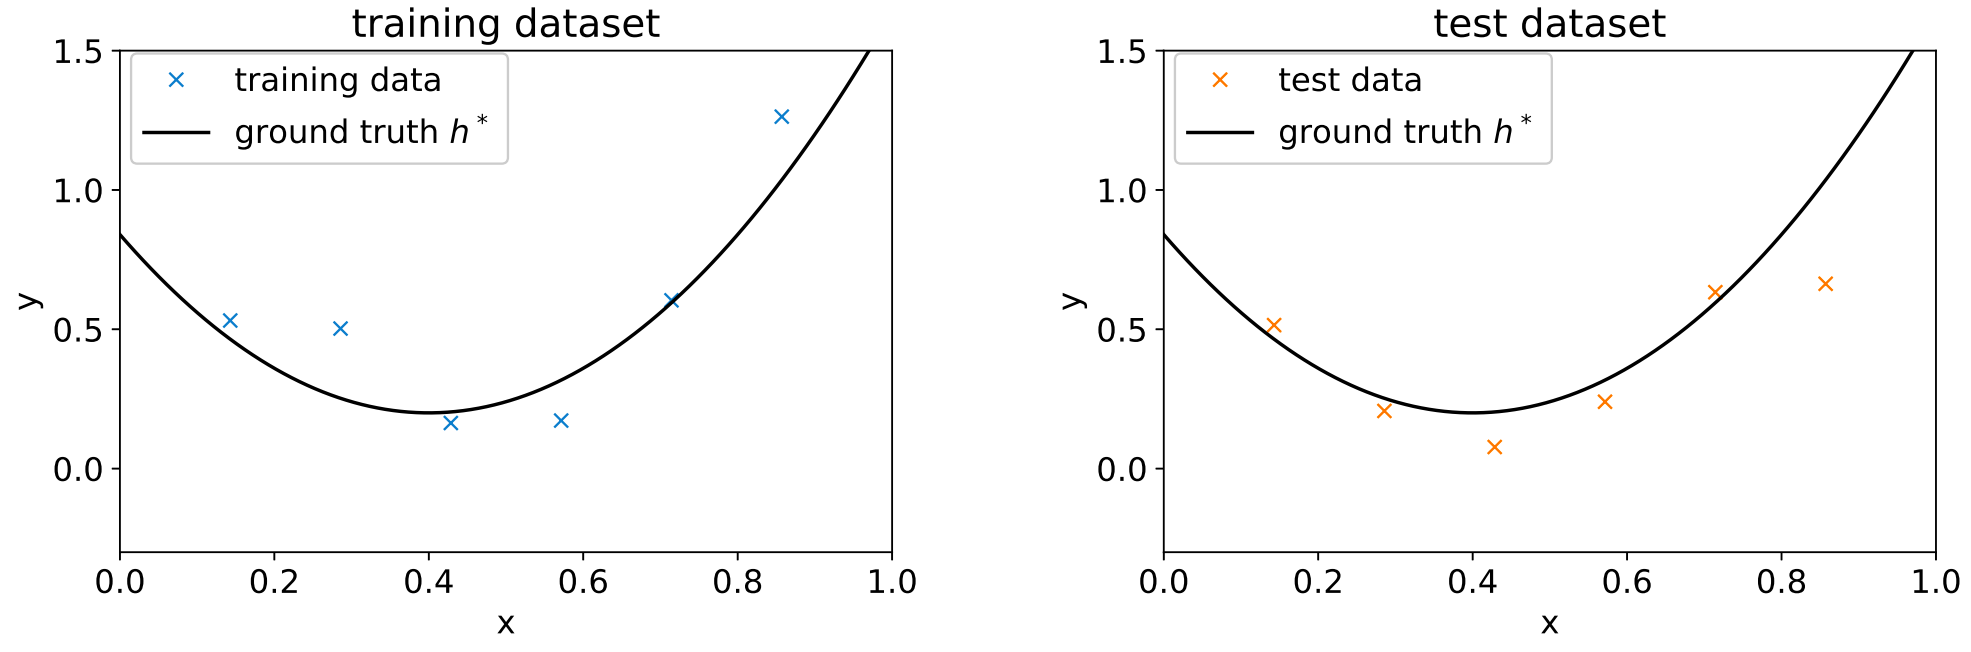
\includegraphics[width=0.8\linewidth]{figs/fitting_gt.png}
    \caption{用于本节的一个训练数据集和测试数据集的示例}
    \label{fig:8.1}
\end{figure}

作为说明性示例,考虑图 \ref{fig:8.1} 所示的训练数据集和测试数据集。训练输入 $x^{(i)}$ 是随机选择的,输出 $y^{(i)}$ 由 $y^{(i)} = h^*(x^{(i)}) + \xi^{(i)}$ 生成,其中函数 $h^*(\cdot)$ 是一个二次函数,在图 \ref{fig:8.1} 中以实线显示,而 $\xi^{(i)}$ 是假定从 $\sim N(0, \sigma^2)$ 生成的观测噪声。测试样本 $(x, y)$ 也有相同的输入-输出关系 $y = h^*(x) + \xi$,其中 $\xi \sim N(0, \sigma^2)$。预测噪声 $\xi$ 是不可能的,因此本质上我们的目标是恢复函数 $h^*(\cdot)$。

将考虑学习各种类型模型的测试误差。在讨论线性回归时,讨论了拟合“简单”模型,例如线性模型 $y = \theta_0 + \theta_1 x$,还是更“复杂”的模型,例如多项式模型 $y = \theta_0 + \theta_1 x + \dots + \theta_5 x^5$ 的问题。

从拟合线性模型开始,如图 \ref{fig:8.2} 所示。即使在训练数据集上,最佳拟合线性模型也无法准确预测 $y$ 与 $x$ 的关系,更不用说在测试数据集上了。这是因为 $y$ 和 $x$ 之间的真实关系不是线性的——任何线性模型都远离真实函数 $h^*(\cdot)$。因此,训练误差很大,这是\textit{欠拟合}的典型情况。

\begin{figure}[H]
    \centering
    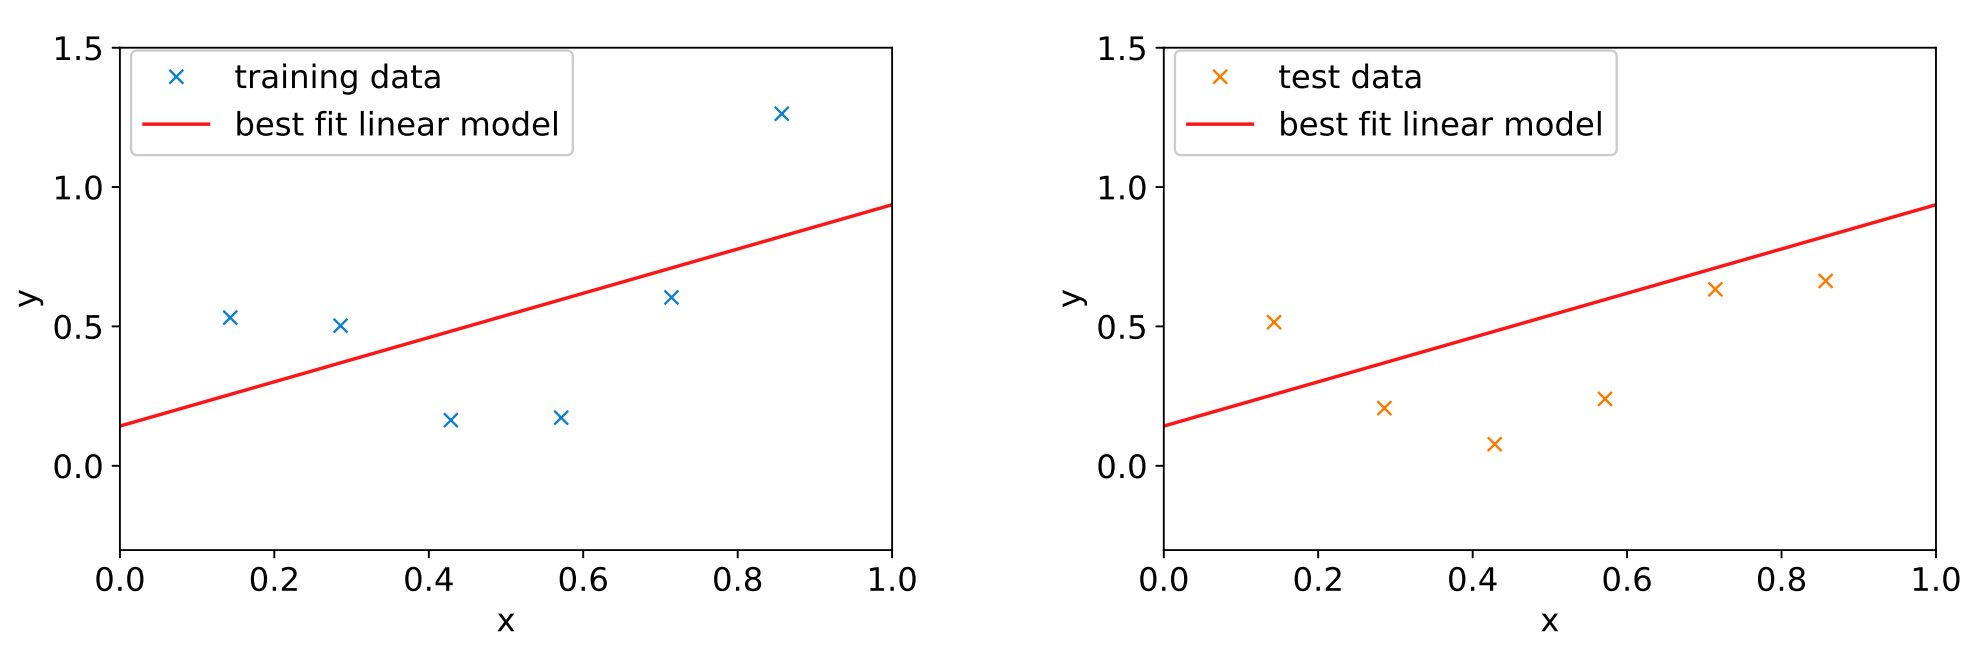
\includegraphics[width=0.8\linewidth]{figs/fitting_linear.png}
    \caption{最好的线性拟合模型也有着巨大的训练和测试误差。}
    \label{fig:8.2}
\end{figure}

\begin{figure}[H]
    \centering
    \begin{minipage}{0.475\linewidth}
        \centering
        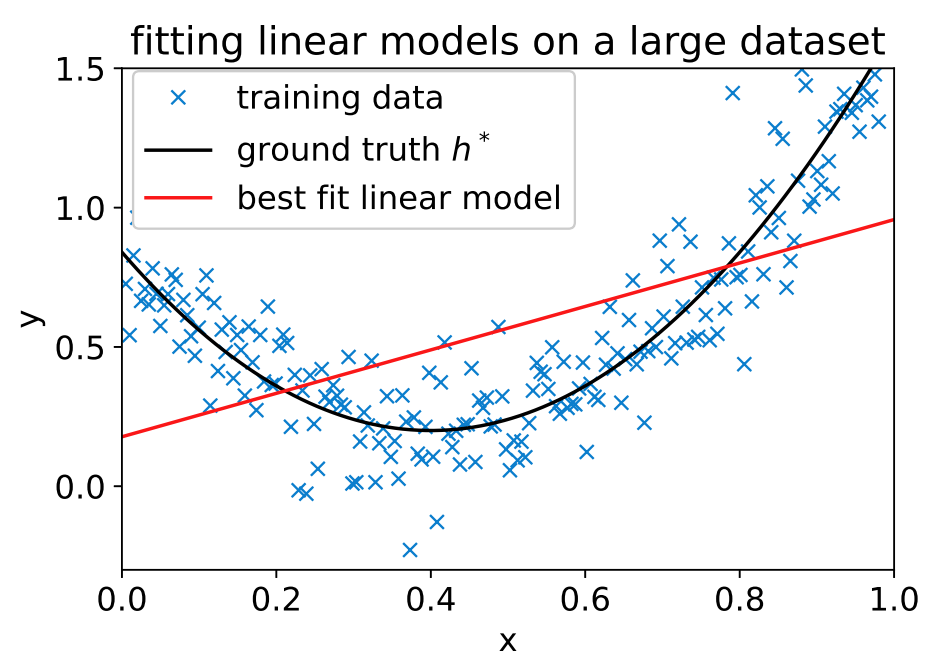
\includegraphics[{width=0.85\linewidth}]{figs/fitting_large.png}
        \caption{最好的线性拟合模型在超大训练集上也有着巨大的训练误差。}
        \label{fig:8.3}
    \end{minipage}\quad
    \begin{minipage}{0.475\linewidth}
        \centering
        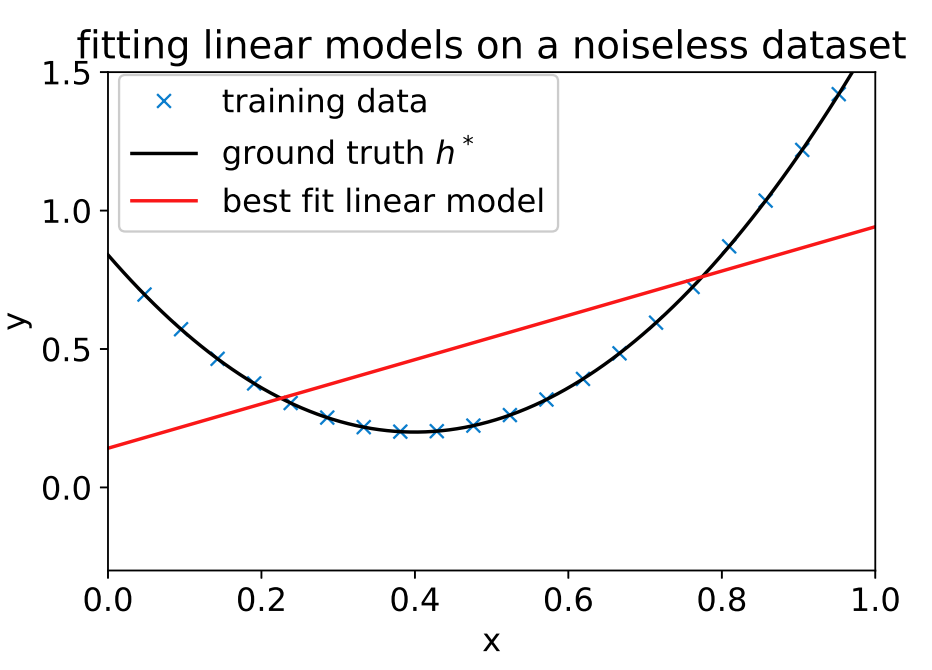
\includegraphics[width=0.85\linewidth]{figs/fitting_noiseless.png}
        \caption{最好的线性拟合模型在没有噪声的训练集上也有着巨大的训练和测试误差。}
        \label{fig:8.4}
    \end{minipage}
\end{figure}

这个问题不能通过增加训练样本来缓解——即使有非常大量的,甚至无限的训练样本,最佳拟合的线性模型仍然不准确,并且无法捕捉数据的结构(图 \ref{fig:8.3})。即使训练数据中不存在噪声,问题仍然存在(图 \ref{fig:8.4})。因此,这里的根本瓶颈在于线性模型族无法捕捉数据中的结构——线性模型无法表示真实的二次函数 $h^*$——而不是缺乏数据。非正式地,我们将模型的\textbf{偏差 (bias)} 定义为即使我们将其拟合到非常大(例如,无限大)的训练数据集时的测试误差。因此,在这种情况下,线性模型具有较大的偏差,并且欠拟合(即无法捕捉数据所表现出的结构)。

接下来,我们将一个 5 次多项式拟合到数据。图 \ref{fig:8.5} 表明它也未能学习到一个好的模型。然而,其失败模式与线性模型的情况不同。具体来说,尽管学习到的 5 次多项式在预测训练样本的 $y^{(i)}$ 与 $x^{(i)}$ 时表现非常好,但在测试样本上效果不佳(图 \ref{fig:8.5})。换句话说,从训练集学习到的模型无法很好地\textit{泛化 (generalize)} 到其他测试样本——测试误差很高。与线性模型的行为相反,5 次多项式的偏差较小——如果我们将 5 次多项式拟合到非常大的数据集,得到的模型将接近二次函数并且也很准确(图 \ref{fig:8.6})。这是因为 5 次多项式族包含所有二次函数(将 $\theta_5 = \theta_4 = \theta_3 = 0$ 设置为零即可得到二次函数),因此,原则上 5 次多项式能够捕捉数据的结构。

\begin{figure}[H]
    \centering
    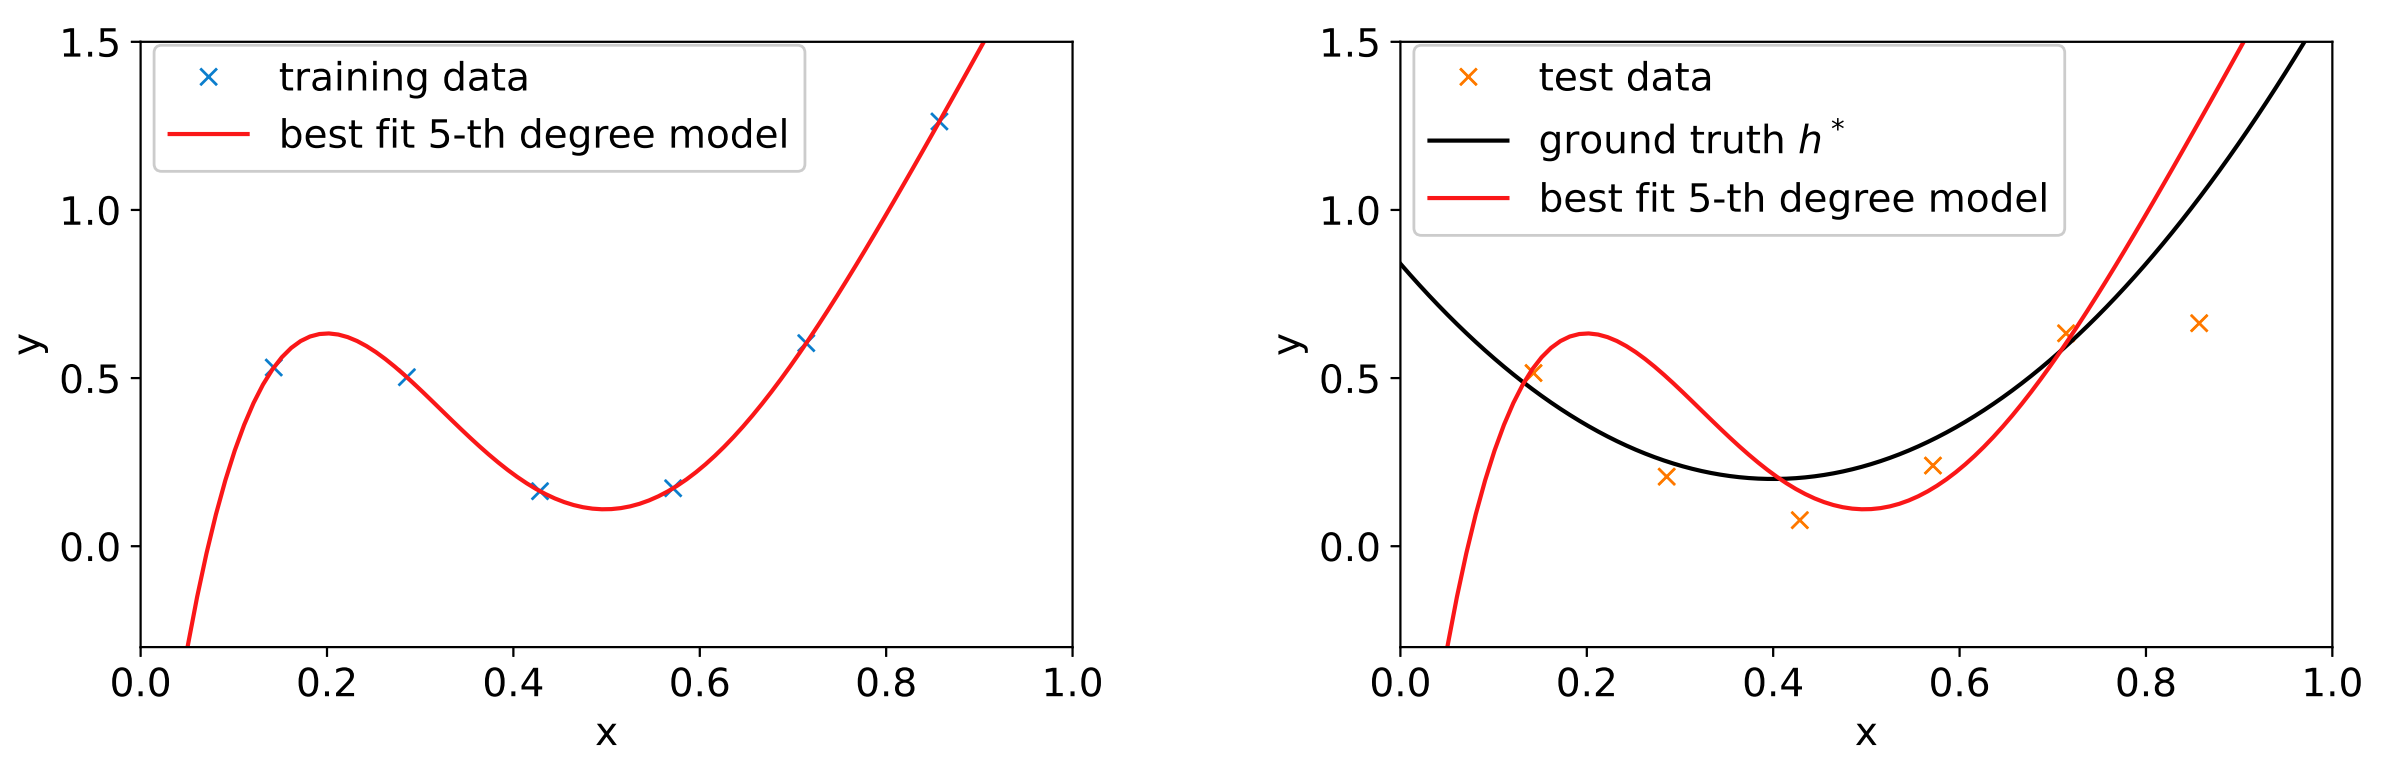
\includegraphics[width=0.8\linewidth]{figs/fitting_5th.png}
    \caption{最佳的 5 次多项式拟合模型训练误差为零,但测试误差仍然很大,并且未能恢复真实情况。这是经典的过拟合情形。}
    \label{fig:8.5}
\end{figure}

\begin{figure}[H]
    \centering
    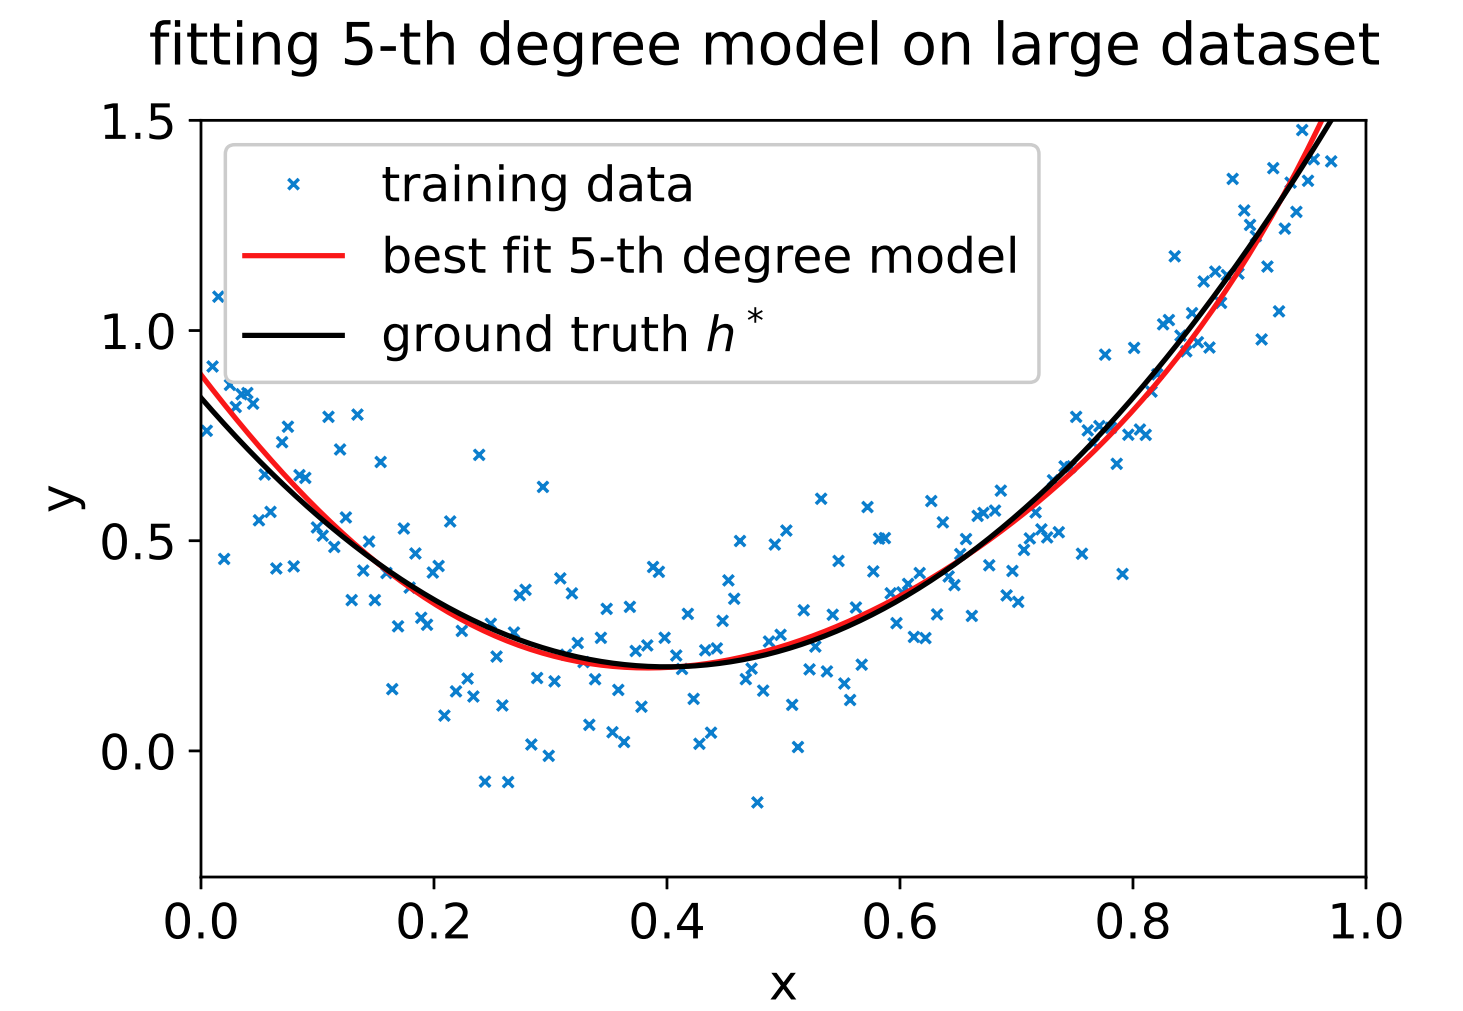
\includegraphics[width=0.5\linewidth]{figs/fitting_5th_large.png}
    \caption{在大型数据集上拟合的最佳 5 次多项式几乎恢复了真实情况——这表明图 \ref{fig:8.5} 中的问题是方差(或数据不足)而不是偏差。}
    \label{fig:8.6}
\end{figure}

拟合 5 次多项式的失败可以用测试误差的另一个组成部分来解释,称为模型拟合过程的\textbf{方差 (variance)}。具体来说,如图 \ref{fig:8.7} 所示,在拟合 5 次多项式时,存在很大的风险,即我们拟合了数据中恰好存在于我们\textit{小而有限 (small, finite)} 的训练集中的模式,但这些模式并不能反映 $x$ 和 $y$ 之间关系的更广泛模式。训练集中的这些“虚假”模式(大部分)是由于观测噪声 $\xi^{(i)}$ 引起的,拟合这些虚假模式会导致模型具有较大的测试误差。在这种情况下,我们称模型具有较大的方差。

\begin{figure}[H]
    \centering
    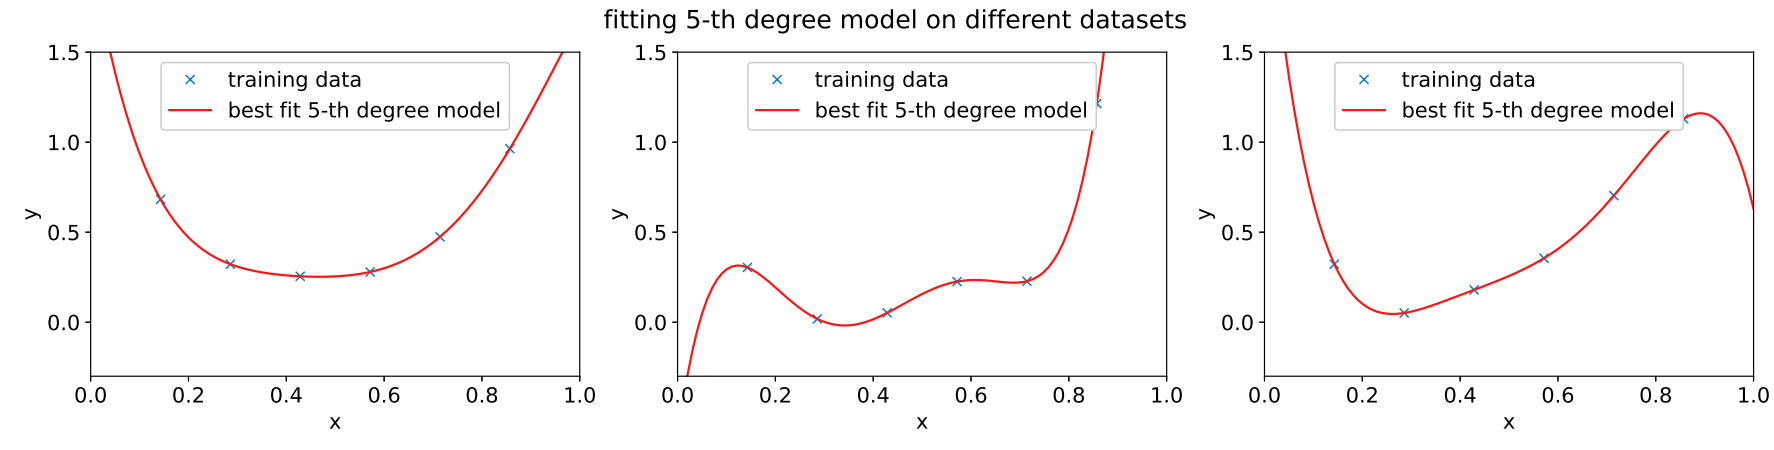
\includegraphics[width=0.95\linewidth]{figs/fitting_5th_different.png}
    \caption{在三个从同一分布产生的不同数据集上拟合的最佳 5 次多项式表现出极大不同,揭示其存在的巨大方差。}
    \label{fig:8.7}
\end{figure}

方差可以直观地(以及数学上证明,如第 \ref{sec:8.1.1} 节所示)通过在多个不同的训练数据集(从相同的潜在分布中抽取)上学习到的模型之间的变化量来表征。“虚假模式”是特定于特定数据集中的噪声(和输入)的随机性,因此在多个训练数据集之间是不同的。因此,对多个数据集的“虚假模式”过拟合应该会导致非常不同的模型。实际上,如图 \ref{fig:8.7} 所示,在三个不同训练数据集上学习到的模型差异很大,对每个数据集的“虚假模式”都存在过拟合。通常,偏差和方差之间存在权衡。如果我们的模型过于“简单”且参数很少,那么它可能具有较大的偏差(但方差较小),并且通常会遭受欠拟合。如果它过于“复杂”且参数很多,那么它可能遭受较大的方差(但偏差较小),因此会过拟合。图 \ref{fig:8.8} 展示了偏差和方差之间典型的权衡关系。

\begin{figure}[H]
    \centering
    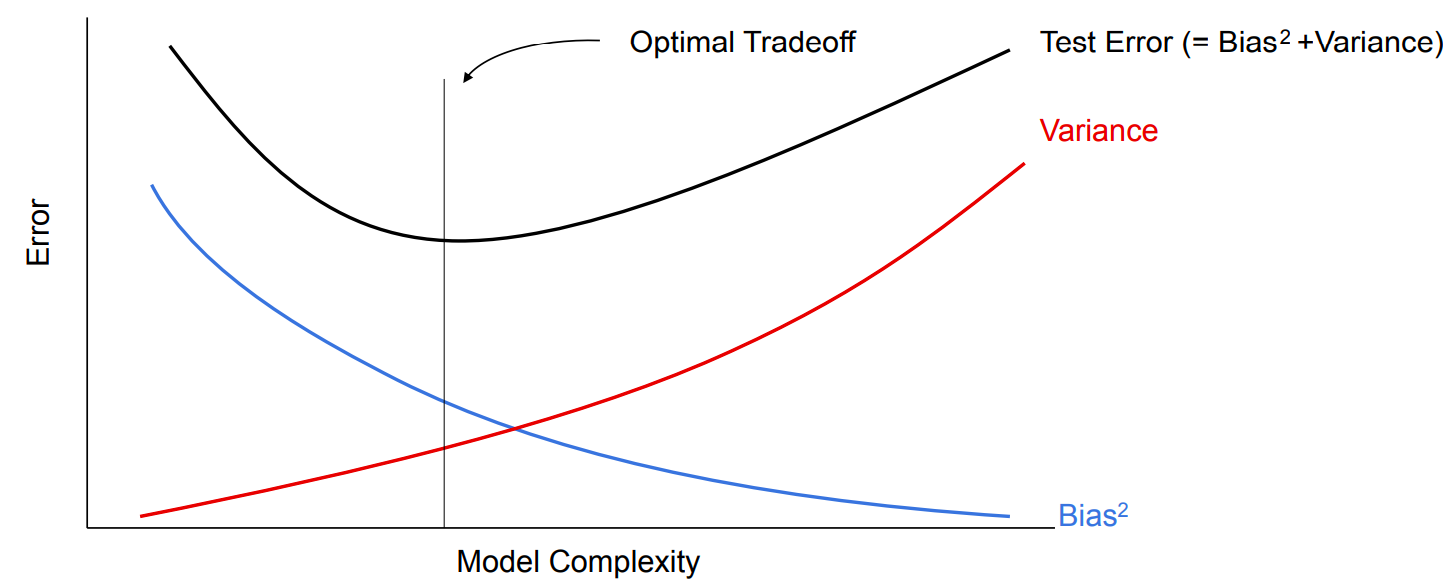
\includegraphics[width=0.9\linewidth]{figs/bias-variance_tradeoff.png}
    \caption{典型的偏差-方差权衡示意图。}
    \label{fig:8.8}
\end{figure}

正如我们将在第 \ref{sec:8.1.1} 节中正式看到的,测试误差可以分解为偏差和方差之和。这意味着随着模型复杂度的增加,测试误差将呈现凸曲线,在实践中我们应该调整模型复杂度以达到最佳权衡。例如,在上面的例子中,拟合二次函数比拟合一次或五次多项式效果更好,如图 \ref{fig:8.9} 所示。

\begin{figure}[H]
    \centering
    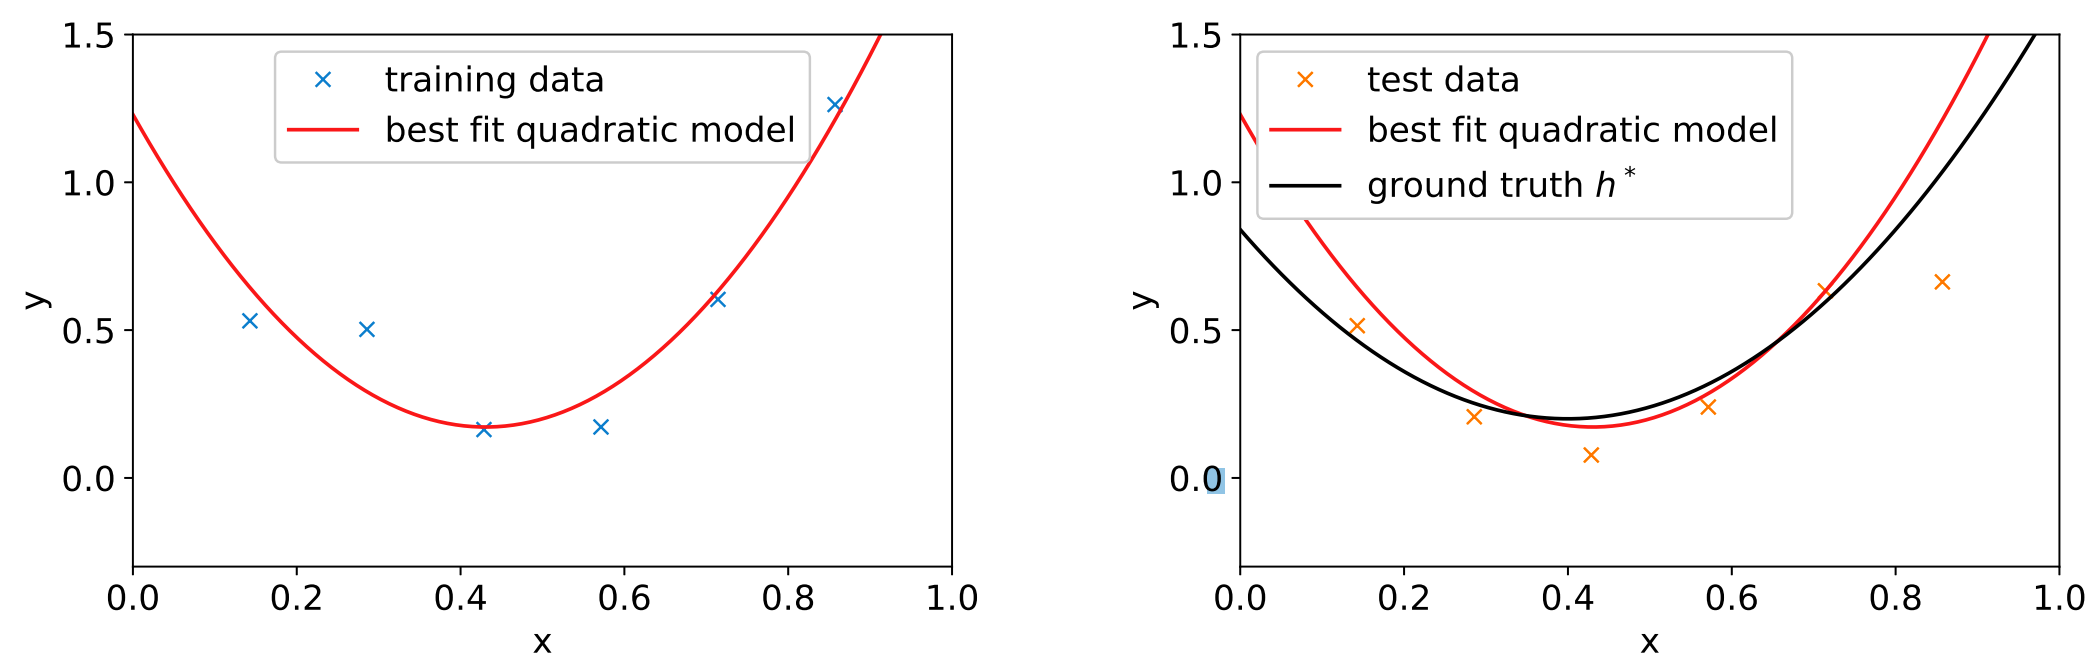
\includegraphics[width=0.8\linewidth]{figs/fitting_quadratic.png}
    \caption{最佳的二次拟合模型的训练误差和测试误差都很小,因为二次模型达到了良好的偏差-方差权衡。}
    \label{fig:8.9}
\end{figure}

有趣的是,偏差-方差权衡曲线或测试误差曲线并不普遍遵循图 \ref{fig:8.8} 中的形状,至少当模型复杂度仅通过参数数量衡量时并非如此。(我们将在 \ref{sec:8.2} 节中讨论所谓的双下降现象。)尽管如此,偏差-方差权衡原理在分析和预测测试误差的行为时,可能仍然是首选方法。

\subsection{(对于回归问题的)数学分解}\label{sec:8.1.1}

为了形式化回归问题的偏差-方差权衡,我们考虑如下设置(这是 \ref{sec:8.1} 节开头段落的扩展)
\begin{itemize}
    \item 抽取一个训练数据集 $S = \{x^{(i)}, y^{(i)}\}_{i=1}^n$,其中 $y^{(i)} = h^*(x^{(i)}) + \xi^{(i)}$ 且 $\xi^{(i)} \in N(0, \sigma^2)$。
    \item 在数据集 $S$ 上训练一个模型,记为 $\hat{h}_S$。
    \item 取一个测试样本 $(x, y)$,使得 $y = h^*(x) + \xi$ 且 $\xi \sim N(0, \sigma^2)$,并测量测试误差的期望(在随机抽取的训练集 $S$ 和随机的 $\xi$ 上进行平均)\footnote{为简单起见,这里测试输入 $x$ 被视为固定,但在对 $x$ 进行平均时,同样的思想仍然成立。}\footnote{期望符号下的下标是为了强调在期望运算中被视为随机的变量。}。
\end{itemize}
\begin{equation}
    \text{MSE}(x) = \mathbb{E}_{S, \xi}[(y - \hat{h}_S(x))^2] \label{eq:8.2}
\end{equation}

我们将把 MSE 分解为偏差项和方差项。我们从一个简单的数学工具开始,该工具将在下面使用两次。

\begin{claim}\label{claim:8.1.1}
    假设 $A$ 和 $B$ 是两个独立的实随机变量,且 $\mathbb{E}[A] = 0$。则 $\mathbb{E}[(A + B)^2] = \mathbb{E}[A^2] + \mathbb{E}[B^2]$。\\
    推论:因为随机变量 $A$ 与常数 $c$ 独立,当 $\mathbb{E}[A] = 0$ 时,我们有 $\mathbb{E}[(A+c)^2] = \mathbb{E}[A^2] + c^2$。
\end{claim}

断言的证明通过展开平方项得出:$\mathbb{E}[(A + B)^2] = \mathbb{E}[A^2 + B^2 + 2AB] = \mathbb{E}[A^2] + \mathbb{E}[B^2] + 2\mathbb{E}[AB] = \mathbb{E}[A^2] + \mathbb{E}[B^2]$。这里我们使用了独立性来证明 $\mathbb{E}[AB] = \mathbb{E}[A]\mathbb{E}[B] = 0$。
使用断言 \ref{claim:8.1.1},令 $A = \xi$ 且 $B = h^*(x) - \hat{h}_S(x)$,我们有
\begin{align}
    \text{MSE}(x) = \mathbb{E}[(y - \hat{h}_S(x))^2] &= \mathbb{E}[(\xi + (h^*(x) - \hat{h}_S(x)))^2] \label{eq:8.3} \\
    &= \mathbb{E}[\xi^2] + \mathbb{E}[(h^*(x) - \hat{h}_S(x))^2] \quad (\text{根据断言 \ref{claim:8.1.1}})  \nonumber\\
    &= \sigma^2 + \mathbb{E}[(h^*(x) - \hat{h}_S(x))^2] \label{eq:8.4}
\end{align}

然后,我们定义 $h_{\text{avg}}(x) = \mathbb{E}_S[\hat{h}_S(x)]$ 为“平均模型”——通过抽取无限多个数据集,并在其上进行训练,然后对它们在 $x$ 上的预测进行平均而获得的模型。注意,$h_{\text{avg}}$ 是一个用于分析目的的假设模型,它在现实中无法获得(因为我们无法拥有无限多个数据集)。结果表明,对于许多情况,$h_{\text{avg}}$(近似)等于在具有无限样本的单个数据集上训练得到的模型。因此,我们也可以直观地解释 $h_{\text{avg}}$,这与我们在上一小节中对偏差的直观定义一致。

我们可以通过令 $c = h^*(x) - h_{\text{avg}}(x)$(这是一个不依赖于 $S$ 选择的常数)和 $A = h_{\text{avg}}(x) - \hat{h}_S(x)$ 来进一步分解 $\text{MSE}(x)$,这符合断言 \ref{claim:8.1.1} 的推论:

\begin{align}
    \text{MSE}(x) &= \sigma^2 + \mathbb{E}[(h^*(x) - \hat{h}_S(x))^2] \label{eq:8.5} \\
    &= \sigma^2 + \mathbb{E}[(h^*(x) - h_{\text{avg}}(x) + h_{\text{avg}}(x) - \hat{h}S(x))^2] \label{eq:8.6} \\
    &= \underbrace{\sigma^2}_{\text{不可避免}} + \underbrace{(h^*(x) - h_{\text{avg}}(x))^2}_{\text{偏差}^2} + \underbrace{\text{var}(\hat{h}S(x))}_{\text{方差}} \label{eq:8.7}
\end{align}
我们将第二项称为偏差(平方),第三项称为方差。如前所述,偏差捕捉了由于模型表达能力不足而引入的误差部分。回想一下,$h_{\text{avg}}$ 可以被认为是即使在无限数据下学习到的最佳可能模型。因此,偏差并非根本上由数据不足引起,而是由模型族本身无法很好地近似 $h^*$ 造成的。例如,在图 \ref{fig:8.2} 所示的例子中,由于任何线性模型都无法近似真实的二次函数 $h^*$,因此 $h_{\text{avg}}$ 也不能,从而偏差项很大。
方差项捕捉了有限数据集的随机性如何引入学习模型中的误差。它衡量了学习模型对数据集中随机性的敏感度。随着数据集大小的增加,方差通常会减小。
对于第一项 $\sigma^2$,我们无能为力,因为根据定义,我们无法预测噪声 $\xi$。
最后,我们注意到,分类问题的偏差-方差分解远不如回归问题清晰。已经有一些提案,但对于什么是“正确”和/或最有用的形式还没有达成一致。


\section{双下降现象}\label{sec:8.2}

\subsection*{模型层面的双下降现象}

最近的研究表明,在包括线性模型和深度神经网络在内的一系列机器学习模型中,测试误差会呈现出一种“双下降”现象\footnote{该现象的发现可能可以追溯到 \cite{opper1995statistical,opper2001learning},最近由 \cite{belkin2020two,hastie2022surprises} 推广。}。正如 \ref{sec:8.1} 节中所讨论的传统观点是,随着模型复杂度的增加,测试误差先下降然后上升,如图 \ref{fig:8.8} 所示。然而,在许多情况下,我们经验性地观察到测试误差可以有第二次下降——它先下降,然后在大到足以很好地拟合所有训练数据时达到峰值附近,然后在所谓的过参数化区域再次下降,其中参数数量大于数据点数量。图 \ref{fig:8.10} 展示了测试误差随模型复杂度(由参数数量衡量)变化的典型曲线。在某种程度上,过参数化区域的第二次下降被认为是机器学习领域的新发现——部分原因是轻度正则化的过参数化模型在深度学习时代得到了广泛应用。这种现象的一个实际意义是,不应回避扩大模型规模和尝试过参数化模型,因为测试误差很可能再次下降到比之前的最低点更低的水平。实际上,在许多情况下,更大的过参数化模型总是能带来更好的测试性能(这意味着第二次下降之后不会出现第二次上升)。

\begin{figure}[H]
    \centering
    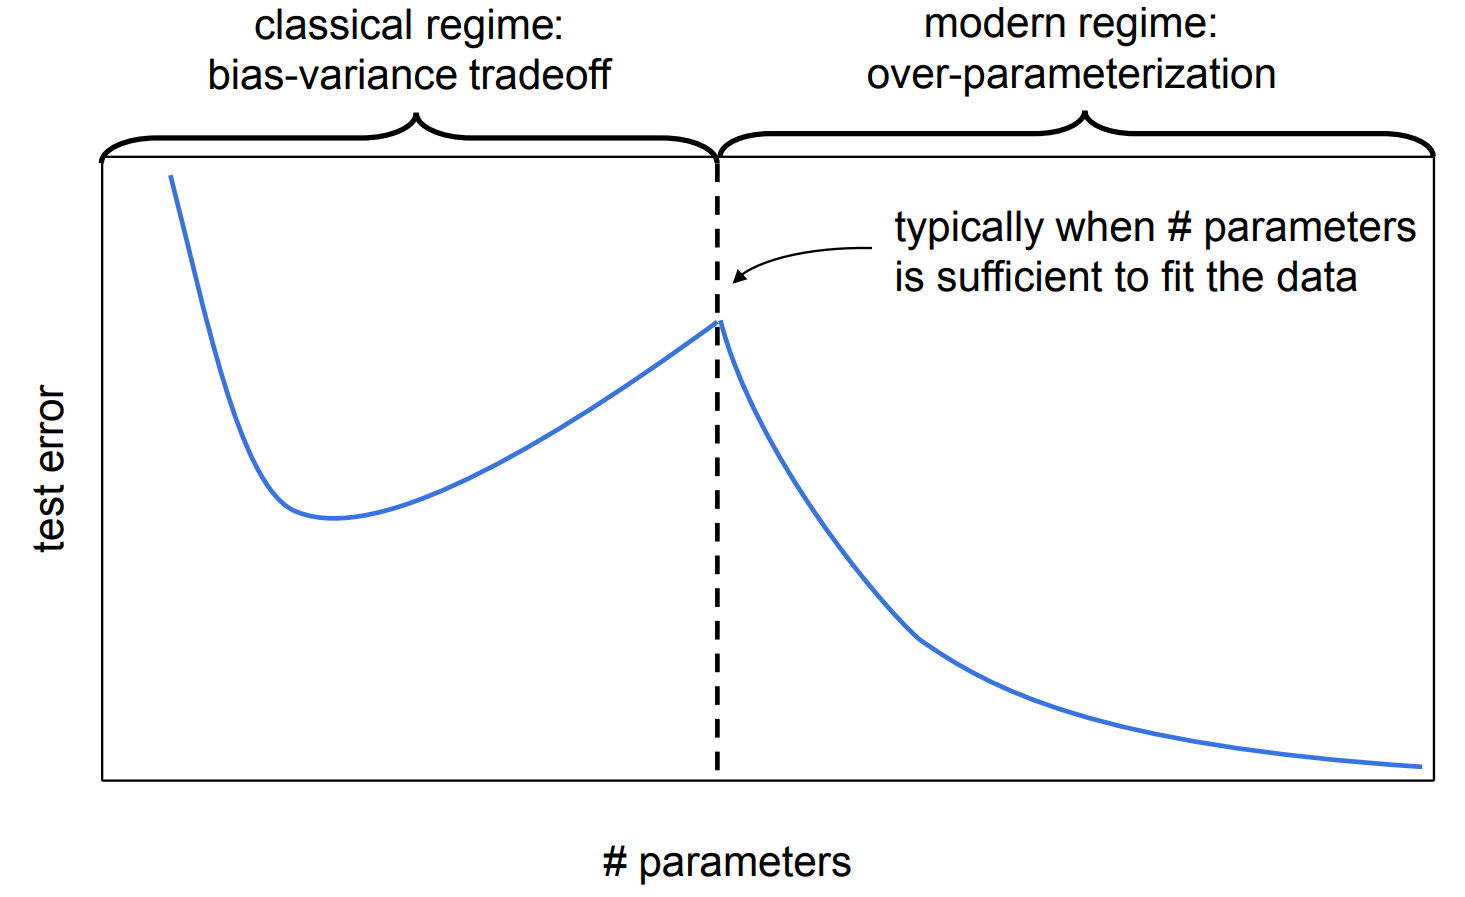
\includegraphics[width=0.8\linewidth]{figs/double_descent.png}
    \caption{典型的模型层面双下降现象。随着参数数量的增加,当参数数量小于训练数据时,测试误差先下降。然后在过参数化区域,测试误差再次下降。}
    \label{fig:8.10}
\end{figure}

\subsection*{样本层面的双下降现象}

从先验知识来看,我们期望更多的训练样本总是能带来更小的测试误差——更多的样本为算法提供了更严格的信息来学习。然而,最近的研究 [\cite{nakkiran2019more}] 观察到,随着样本数量的增加,测试误差并非单调递减。相反,如图 \ref{fig:8.11} 所示,测试误差先下降,然后在样本数量(记为 $n$)与参数数量(记为 $d$)接近时增加并达到峰值,然后再次下降。我们将此称为样本层面的双下降现象。在某种程度上,样本层面的双下降和模型层面的双下降本质上描述的是类似的现象——测试误差在 $n \approx d$ 时达到峰值。

\begin{figure}[H]
    \centering
    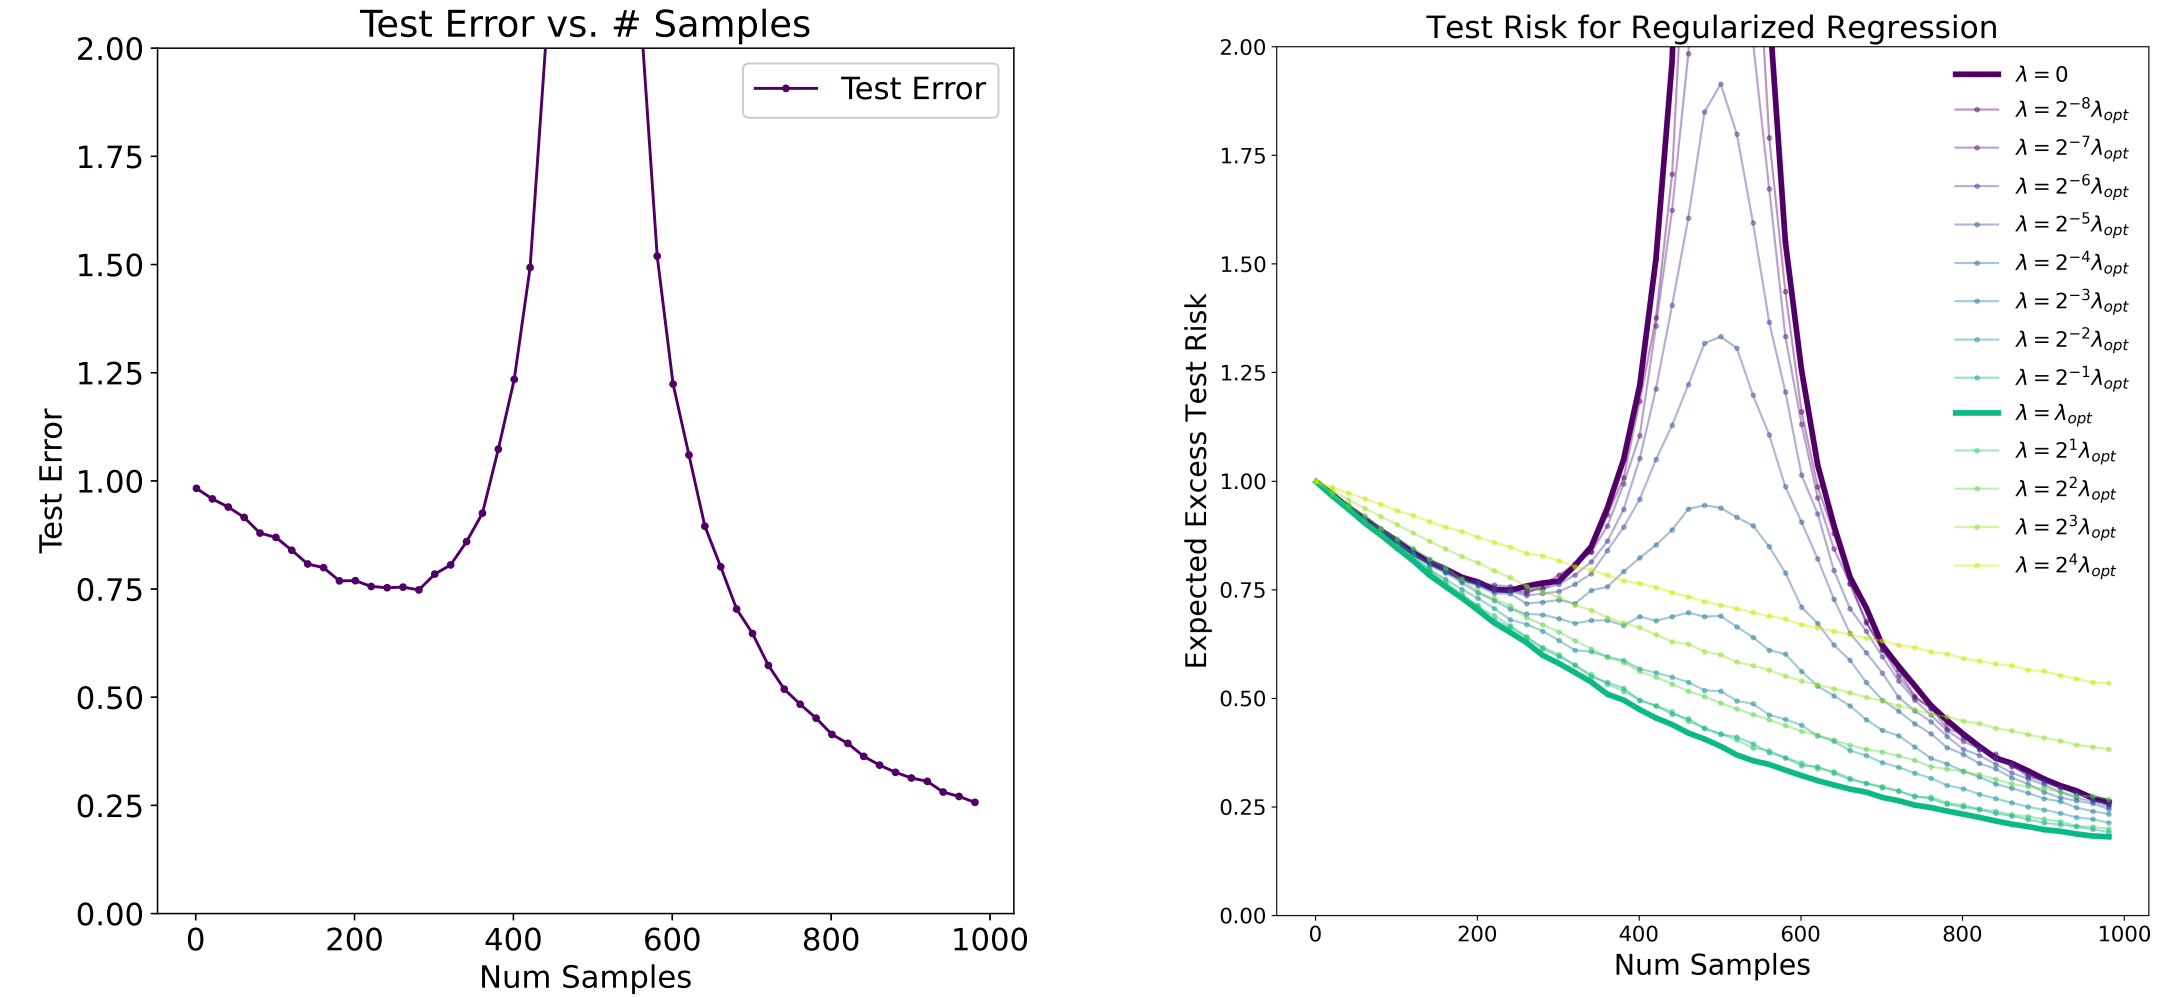
\includegraphics[width=0.9\linewidth]{figs/sample_double_descent.png}
    \caption{\textbf{左:}线性模型在样本层面的双下降现象。\textbf{右:}不同正则化强度下线性模型在样本层面的双下降现象。 使用最优正则化参数(对每个 $n$ 都调到最优,以绿色实线显示)缓解双下降。 \textbf{设置:}$(x, y)$ 的数据分布为 $x \sim \mathcal{N}(0, I_d)$ 且 $y \sim x^\top \beta + \mathcal{N}(0, \sigma^2)$,其中 $d = 500$, $\sigma = 0.5$ 且 $\|\beta\|_2 = 1$.\protect\footnotemark}
    \label{fig:8.11}
\end{figure}
\footnotetext[8]{此图依照 \cite{nakkiran2020optimal} 的图 1 复现,类似的现象也可以在 \cite{hastie2022surprises,mei2022generalization} 中观察到。}

\subsection*{解释和缓解策略}

样本层面的双下降,特别是测试误差在 $n \approx d$ 处的峰值,表明在这些实验中评估的现有训练算法在 $n \approx d$ 时远非最优。我们可以通过丢弃一些样本,使用较小的样本量运行算法来避免峰值。换句话说,原则上存在其他算法可以在 $n \approx d$ 时实现更小的测试误差,但这些实验中评估的算法未能做到。学习过程的次优性似乎是样本层面和模型层面双下降峰值的罪魁祸首。
实际上,通过最优调整的正则化(将在第 \ref{chapter:9} 章中更详细讨论),在 $n \approx d$ 区域的测试误差可以显著改善,并且模型层面和样本层面的双下降现象都得到了缓解。参见图 \ref{fig:8.11}。
上述直觉只解释了模型层面和样本层面双下降的峰值,但没有解释模型层面双下降的第二次下降——为什么过参数化模型能够很好地泛化。对过参数化模型的理论理解是一个活跃的研究领域,最近取得了许多进展。一个典型的解释是,常用的优化器(如梯度下降)提供了隐式正则化效应(将在第 9.2 节中更详细讨论)。换句话说,即使在过参数化区域且使用了非正则化的损失函数,模型仍然隐式地进行了正则化,因此表现出比拟合数据的任意解更好的测试性能。例如,对于线性模型,当 $n \ll d$ 时,使用零初始化进行梯度下降的优化器会找到拟合数据的\textit{最小范数 (minimum norm)} 解(而不是拟合数据的任意解),而最小范数正则化器对于过参数化区域来说是一个足够好的正则化器(但在 $n \approx d$ 时不是一个好的正则化器,导致测试误差达到峰值)。

\begin{figure}[H]
    \centering
    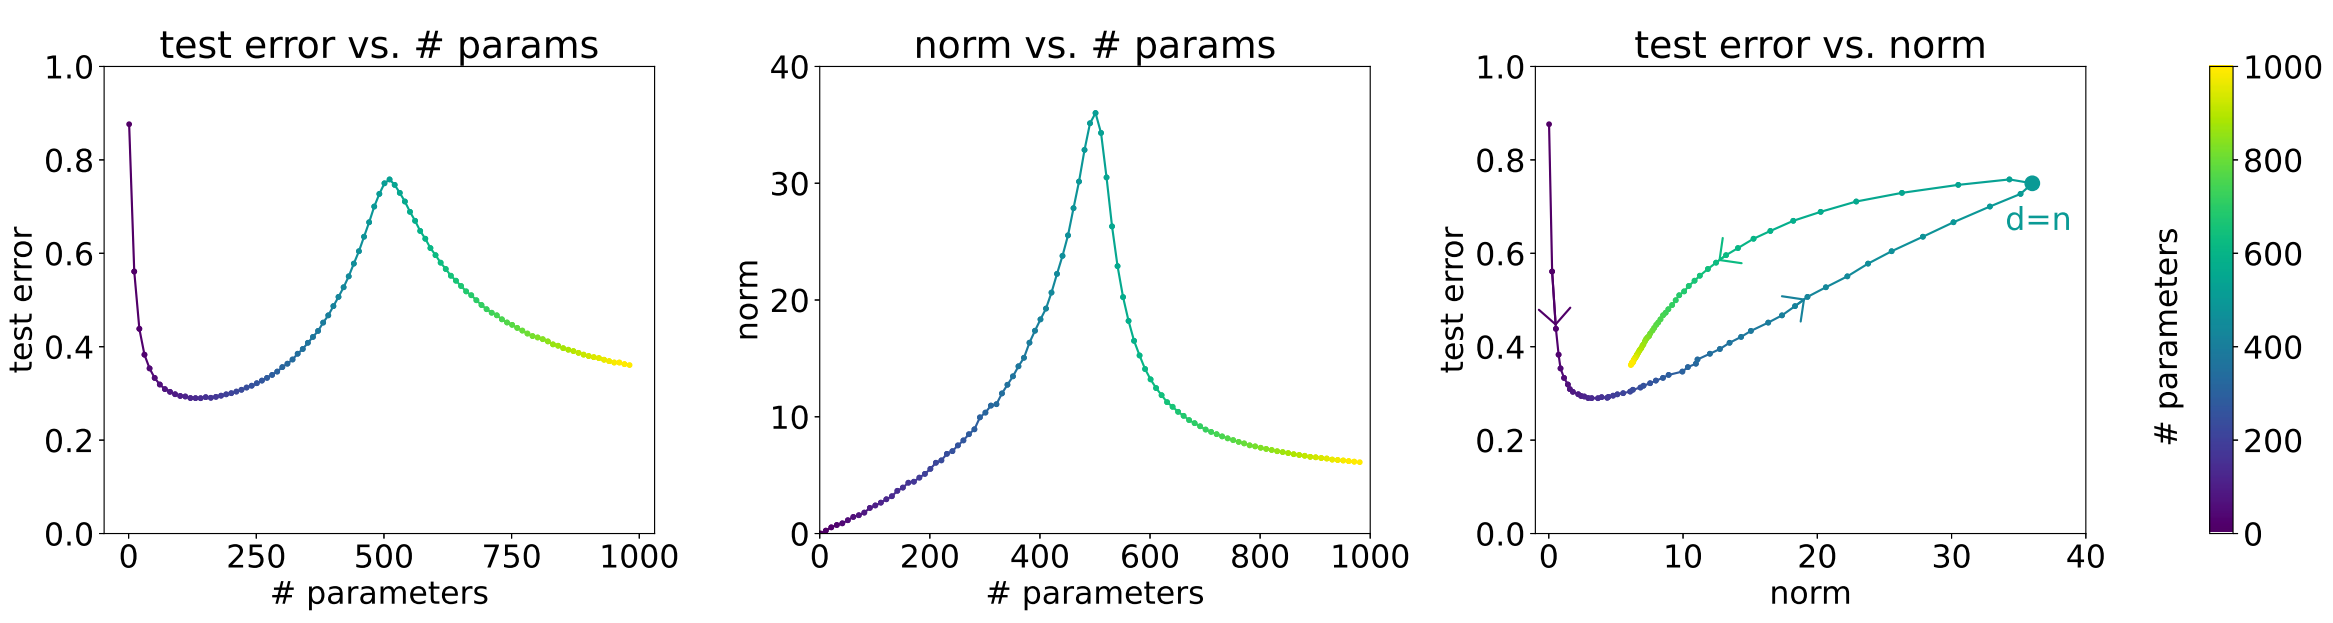
\includegraphics[width=1.0\linewidth]{figs/double_descent_norm.png}
    \caption{\textbf{左:}双下降现象,其中模型复杂度用参数数量来衡量。\textbf{中:}学习到的模型的范数在 $n \approx d$ 附近达到峰值。\textbf{右:}测试误差与学习到的模型范数的关系。颜色条表示参数数量,箭头表示模型尺寸增加的方向。它们的关系更接近于传统认知,而不是双下降。 \textbf{设置}:我们考虑一个样本量固定为 $n = 500$ 的线性回归。输入 $x$ 是 Fashion-MNIST 上的随机 ReLU 特征,输出 $y \in \mathbb{R}^{10}$ 是 one-hot 标签。这与 \cite{nakkiran2020optimal} 第 5.2 节中的设置相同。}
    \label{fig:8.12}
\end{figure}

最后,我们还要指出,双下降现象主要在模型的复杂度用参数数量来衡量时被观察到。参数数量是否以及何时是衡量模型复杂度的最佳指标尚不清楚。例如,在许多情况下,模型的范数被用作复杂度度量。如图 \ref{fig:8.12} 右图所示,对于一个特定的线性情况,如果我们绘制测试误差与学习到的模型范数的关系,双下降现象就不再发生。这部分是因为学习到的模型的范数在 $n \approx d$ 附近也达到峰值(参见图 \ref{fig:8.12}(中)或 \cite{belkin2019reconciling}、\cite{mei2022generalization},以及 \cite{james2021introduction} 在第 10.8 节中的讨论)。对于深度神经网络,正确的复杂度度量更加难以捉摸。双下降现象的研究仍是一个活跃的研究课题。

\section{样本复杂度边界 (选读)}\label{sec:8.3}



\chapter{正则化与模型选择}\label{chapter:9}

\section{正则化}\label{sec:9.1}

回顾第 \ref{sec:8.1} 节中讨论的,过拟合通常是由于使用了过于复杂的模型导致的,我们需要选择适当的模型复杂度以达到最优的偏差-方差权衡。当模型复杂度用参数数量衡量时,我们可以改变模型的规模(例如,神经网络的宽度)。然而,衡量模型复杂度的正确且有信息量的方式可以是参数的函数(例如,参数的 $\ell_2$ 范数),这可能不一定取决于参数的数量。在这种情况下,我们将使用正则化,这是一种重要的机器学习技术,用于控制模型复杂度并防止过拟合。

正则化通常涉及在训练损失/代价函数中添加一个附加项,称为正则项,这里用 $R(\theta)$ 表示:
\begin{equation}
    J_\lambda(\theta) = J(\theta) + \lambda R(\theta)
    \label{eq:9.1}
\end{equation}
这里,$J_\lambda$ 通常被称为正则化损失,$\lambda \geq 0$ 被称为正则化参数。正则项 $R(\theta)$ (在几乎所有情况下)是一个非负函数。在经典方法中,$R(\theta)$ 纯粹是参数 $\theta$ 的函数,但一些现代方法允许 $R(\theta)$ 依赖于训练数据集。\footnote{为了简洁起见,这里的记号省略了对训练数据集的依赖性——$J(\theta)$ 显然需要依赖于训练数据集。}

正则项 $R(\theta)$ 通常被选择为衡量模型 $\theta$ 复杂度的某种度量。因此,在使用正则化损失时,我们的目标是找到一个既能很好地拟合数据(即具有小的损失 $J(\theta)$)又具有小的模型复杂度(即小的 $R(\theta)$)的模型。这两个目标之间的平衡由正则化参数 $\lambda$ 控制。当 $\lambda = 0$ 时,正则化损失等同于原始损失。当 $\lambda$ 是一个足够小的正数时,最小化正则化损失也可以有效地最小化原始损失,同时利用正则项来区分那些原始损失相同的解。当正则项非常大时,原始损失不再有效(并且模型很可能具有很大的偏差)。

最常用的正则化可能是 $\ell_2$ 正则化,其中 $R(\theta) = \frac{1}{2}\|\theta\|_2^2$。它鼓励优化器找到一个 $\ell_2$ 范数较小的模型。在深度学习中,这通常被称为\textbf{权重衰减 (weight decay)},因为在正则化损失上进行学习率为 $\eta$ 的梯度下降,等价于将 $\theta$ 乘以一个标量因子 $1 - \eta\lambda$ 收缩/衰减后,使用标准梯度:
\begin{align}
    \theta &\leftarrow \theta - \eta \nabla J_\lambda(\theta) = \theta - \eta \lambda \theta - \eta \nabla J(\theta) \nonumber \\
    &= \underbrace{(1 - \eta \lambda)\theta}_{\text{权重衰减}} - \eta \nabla J(\theta)
    \label{eq:9.2}
\end{align}

除了鼓励更简单的模型之外,正则化还可以对模型参数施加归纳偏置或结构。例如,假设我们先验地认为真实模型参数中非零项的数量很少\footnote{对于线性模型,这意味着模型只使用输入的少数几个坐标来做出准确的预测。}——这通常被称为模型的稀疏性——就可以对 $\theta$ 的非零项数量施加正则化,记作 $\|\theta\|_0$,从而利用这种先验。施加额外的参数结构会缩小我们的搜索空间,并使模型族的复杂度变小——例如,稀疏模型族可以被认为比所有模型族具有更低的复杂度——因此往往会带来更好的泛化能力。另一方面,强烈施加额外的结构可能会增加偏差的风险。例如,如果强烈地对稀疏性进行正则化,但是稀疏模型不能准确地预测,我们将会遭受很大的偏差(类似于第 \ref{sec:8.1} 节中使用线性模型去学习由二次函数表示的数据的情况)。

参数的稀疏性不是参数的连续函数,因此无法通过(随机)梯度下降对其进行优化。一个常见的松弛方法是使用 $R(\theta) = \|\theta\|_1$ 作为替代。\footnote{存在丰富的理论工作解释了为什么 $\|\theta\|_1$ 是稀疏性的良好替代,但这超出了本课程的范围。直观地说:假设参数在单位球面上,具有最小 $\ell_1$ 范数的参数也碰巧是只有 1 个非零坐标的最稀疏参数。因此,在某种程度上,稀疏性和 $\ell_1$ 范数给出了相同的极值点。}

对于线性模型,$R(\theta) = \|\theta\|_1$(也称为 LASSO)和 $R(\theta) = \frac{1}{2}\|\theta\|_2^2$ 可能是最常用的正则化项。其他范数和范数的幂有时也会被使用。$\ell_2$ 范数正则化在核方法中更为常用,因为 $\ell_1$ 正则化通常与核技巧不兼容(最优解不能写成特征内积的函数)。

在深度学习中,最常用的正则化项是 $\ell_2$ 正则化或权重衰减。其他常见的正则化方法包括 dropout、数据增强、对权重矩阵的谱范数进行正则化以及对模型的 Lipschitz 性进行正则化等。深度学习中的正则化是一个活跃的研究领域,并且我们还知道还有一个隐式的正则化来源,这将在下一节中讨论。

\section{隐式正则化效应 (选读)}\label{sec:9.2}

优化器的隐式正则化效应,或者说隐式偏置或算法正则化,是在深度学习时代观察到的一个新概念/现象。它主要指的是优化器可以在正则化损失所施加的结构之外,隐式地对参数施加结构。

在大多数经典设置中,损失或正则化损失具有唯一的全局最小值,因此任何合理的优化器都应该收敛到该全局最小值,并且不施加任何额外的偏好。然而,在深度学习中,通常损失或正则化损失具有多个(近似)全局最小值,不同的优化器可能收敛到不同的全局最小值。尽管这些全局最小值具有相同或相似的训练损失,但它们的性质可能不同,并且泛化性能也可能显著不同。参见图 9.1 和 9.2 及其说明文字,以了解插图和一些实验结果。例如,某个全局最小值可能比其他全局最小值产生更具 Lipschitz 性或更稀疏的模型,从而具有更好的测试误差。结果表明,许多常用的优化器(或其组成部分)倾向于或偏向于寻找具有某些特性的全局最小值,从而带来更好的测试性能。

\begin{figure}[H]
    \centering
    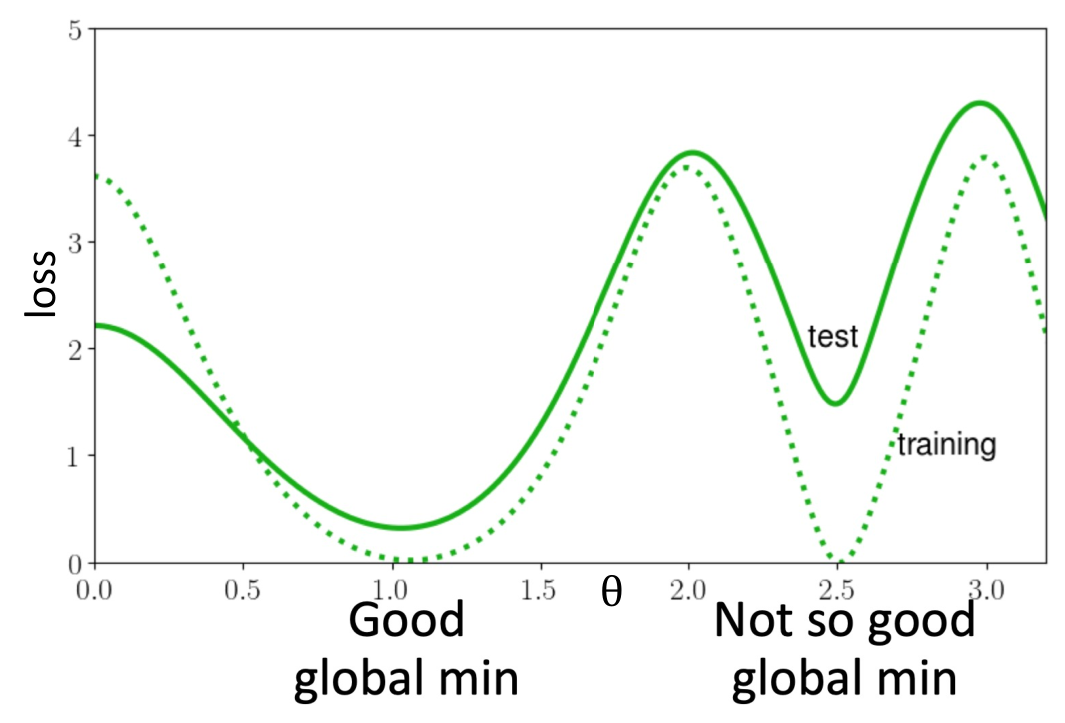
\includegraphics[width=0.6\textwidth]{figs/global_minima.png}
    \caption{在训练损失上的全局最小点的测试性能不相同的图示。}
    \label{fig:9.1}
\end{figure}

\begin{figure}[H]
    \centering
    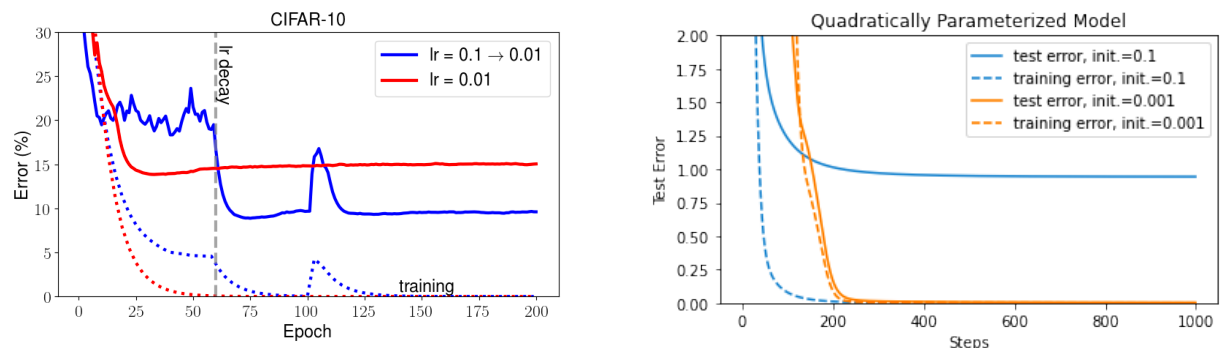
\includegraphics[width=0.9\textwidth]{figs/global_minima_nn.png}
    \caption{\textbf{左:}在 CIFAR-10 数据集上,使用两种不同学习率调度方案训练的神经网络的性能。尽管两个实验使用了完全相同的正则化损失,并且优化器完美地拟合了训练数据,但模型的泛化性能差异很大。\textbf{右}:在另一个合成数据集上,使用不同初始化的优化器具有相同的训练误差,但泛化性能不同。\protect\footnotemark}
\end{figure}
\footnotetext[4]{设置与 \cite{woodworth2020kernel} 和 \cite{haochen2020shape} 一致。}

总而言之,所要传达的关键信息是,优化器的选择不仅影响训练损失的最小化,还施加了隐式正则化并影响模型的泛化能力。即使当前的优化器已经完美地收敛到较小的训练误差,也可能仍然需要调整优化器以获得更好的泛化性能。

人们可能会想知道优化器的哪些组成部分偏向于哪种类型的全局最小值,以及哪种类型的全局最小值可能具有更好的泛化能力。这些是研究人员正在积极探索的开放性问题。经验和理论研究已经提供了一些线索和启发式方法。在许多(但不是全部)情况下,在那些优化能够成功最小化训练损失的设置中,使用较大的初始学习率、较小的初始化、较小的批量大小和动量似乎有助于偏向于更具泛化能力的解。一个猜想(在某些简化情况下可以证明)是,优化过程中的随机性有助于优化器找到更平坦的全局最小值(损失曲率较小的全局最小值),而平坦的全局最小值往往会产生更具 Lipschitz 性和更好泛化能力的模型。形式化地刻画隐式正则化效应仍然是一个具有挑战性的开放性研究问题。

\section{通过交叉验证选择模型}\label{sec:9.3}

假设我们正在为一个学习问题选择几种不同的模型。例如,我们可能正在使用多项式回归模型 $h_\theta(x) = g(\theta_0 + \theta_1 x + \theta_2 x^2 + \dots + \theta_k x^k)$,并希望决定 $k$ 应该取 0, 1, ..., 或 10 中的哪个值。我们如何自动选择一个模型,使其在偏差和方差这对孪生罪恶之间取得良好权衡?\footnote{考虑到我们在之前的笔记中说过偏差和方差是截然不同的两种“野兽”,有些读者可能会想知道我们在这里是否应该称它们为“孪生”罪恶。也许最好将它们视为非同卵双胞胎。不过“偏差和方差这对异卵孪生罪恶”这个短语听起来不太顺口。} 另外,假设我们想自动选择局部加权回归的带宽参数 $\tau$,或者 $\ell_1$ 正则化 SVM 的参数 $C$,该如何做?

为了具体起见,在这些笔记中,我们假设我们有一些有限的模型集合 $\mathcal{M} = \{M_1, \dots, M_d\}$,我们正尝试从中进行选择。例如,在上面的第一个例子中,模型 $M_i$ 将是一个 $i$ 次多项式回归模型。(推广到无限 $\mathcal{M}$ 并不难。\footnote{如果我们正在从无限的模型集合中进行选择,例如对应于带宽 $\tau \in \mathbb{R}^+$ 的所有可能值,我们可以对 $\tau$ 进行离散化,只考虑其有限个可能值。更普遍地,这里描述的大多数算法都可以看作是在模型空间中执行优化搜索,而且我们也可以在无限模型类别上执行这种搜索。})另外,如果我们正在决定是使用 SVM、神经网络还是逻辑回归,那么 $\mathcal{M}$ 可能包含这些模型。

\subsection*{交叉验证}

假设我们像往常一样,给定一个训练集 $S$。考虑到我们对经验风险最小化的了解,以下是基于经验风险最小化进行模型选择的一种初步算法:

\begin{enumerate}
    \item 在 $S$ 上训练每个模型 $M_i$,得到假设 $h_i$。
    \item 选择训练误差最小的假设。
\end{enumerate}

这个算法\textit{不 (not)} 起作用。考虑选择多项式的幂次。多项式的幂次越高,它就越能更好地拟合训练集 $S$,从而训练误差越低。因此,这种方法总是会选择高方差、高幂次的多项式模型,正如之前所述,这通常是一个糟糕的选择。

这里有一个效果更好的算法:叫做\textbf{留出交叉验证 (hold-out cross validation)}(也称为\textbf{简单交叉验证 (simple cross validation)})中,算法执行以下步骤:

\begin{enumerate}
    \item 随机将 $S$ 分割成 $S_{\text{train}}$(例如,70\% 的数据)和 $S_{\text{cv}}$(剩余的 30\%)。这里的 $S_{\text{cv}}$ 称为留出交叉验证集。
    \item 仅在 $S_{\text{train}}$ 上训练每个模型 $M_i$,得到一些假设 $h_i$。
    \item 选择并输出在留出交叉验证集上误差 $\hat{\varepsilon}_{S_{\text{cv}}}(h_i)$ 最小的假设 $h_i$。(这里 $\hat{\varepsilon}_{S_{\text{cv}}}(h)$ 表示假设 $h$ 在 $S_{\text{cv}}$ 中的例子上的平均误差。)留出集上的误差也称为验证误差。
\end{enumerate}

通过在模型未训练过的例子集合 $S_{\text{cv}}$ 上进行测试/验证,我们获得了每个假设 $h_i$ 的真实泛化/测试误差的更好估计。因此,这种方法本质上是选择具有最小估计泛化/测试误差的模型。验证集的大小取决于可用例子的总数。通常,留出交叉验证中使用的验证集数据量占总数据量的 1/4 到 1/3,其中 30\% 是一个典型的选择。然而,当总数据集非常大时,只要验证例子的绝对数量足够多,验证集可以占总例子的一小部分。例如,ImageNet 数据集有大约 1M 训练图像,验证集有时设置为 50K 图像,仅占总例子的约 5\%。

可选地,算法中的步骤 3 也可以替换为根据 $\arg \min_i \hat{\varepsilon}_{S_{\text{cv}}}(h_i)$ 选择模型 $M_i$,然后使用整个训练集 $S$ 重新训练 $M_i$。(这通常是一个好主意,除了一个例外,即对初始条件和/或数据的扰动很敏感的学习算法。对于这些方法,模型 $M_i$ 在 $S_{\text{train}}$ 上表现良好并不一定意味着它在 $S_{\text{cv}}$ 上也会表现良好,并且最好放弃重新训练这一步。)

使用留出交叉验证的缺点是它“浪费”了大约 30\% 的数据。就算我们选择在整个训练集上重新训练,但如果我们试图寻找一个性能良好的模型,却只有 $0.7n$ 个训练样本而不是完整的 $n$ 个训练样本,那么这种“浪费”依然存在。虽然在数据丰富廉价的情况下这很好,但在数据稀缺的情况下(比如 $n=20$ 时),我们希望采取更有效的方法。

这里有一种称为 \textbf{$k$ 折交叉验证 ($k$-fold cross validation)} 的方法,它每次保留更少的数据:

\begin{enumerate}
    \item 随机将 $S$ 分割成 $k$ 个不相交的子集,每个子集包含 $m/k$ 个训练样本。我们将这些子集称为 $S_1, \dots, S_k$。
    \item 对于每个模型 $M_i$,我们按如下方式评估它:
    \begin{itemize}
        \item[] 对于 $j=1, \dots, k$
        \begin{itemize}
            \item[] 在 $S_1 \cup \dots \cup S_{j-1} \cup S_{j+1} \cup \dots \cup S_k$ 上训练模型 $M_i$(即,在除 $S_j$ 外的所有数据上训练),得到一些假设 $h_{ij}$。
            \item[] 在 $S_j$ 上测试假设 $h_{ij}$,得到 $\hat{\varepsilon}_{S_j}(h_{ij})$。
        \end{itemize}
        \item[] 然后,模型 $M_i$ 的估计泛化误差计算为 $\hat{\varepsilon}_{S_j}(h_{ij})$ 的平均值(对 $j$ 取平均)。
    \end{itemize}
    \item 选择估计泛化误差最低的模型 $M_i$,并在整个训练集 $S$ 上重新训练该模型。得到的假设作为最终输出。
\end{enumerate}

这里通常选择的折数是 $k=10$。每次保留的数据比例现在是 $1/k$,比之前小得多——这个过程也可能比留出交叉验证的计算成本更高,因为现在需要对每个模型训练 $k$ 次。

虽然 $k=10$ 是一个常用的选择,但在数据非常稀缺的问题中,有时我们会使用极端的选择 $k=m$,以便每次保留尽可能少的数据。在这种设置下,我们会在 $S$ 中除了一个训练例子之外的所有例子上重复训练,并在那个保留的例子上进行测试。然后将得到的 $m=k$ 个误差平均起来,以获得模型泛化误差的估计。这种方法也有自己的名字,由于我们每次只保留一个训练样本,这种方法称为\textbf{留一交叉验证 (leave-one-out cross validation)}。

最后,虽然我们把这些交叉验证当作选择模型的方法,它们也可以用于评估\textit{单个 (single)} 模型或算法。例如,如果您实现了一些学习算法并想估计它在您的应用程序中的表现如何(或者如果您发明了一种新的学习算法并想在技术论文中报告它在各种测试集上的表现),交叉验证是一种合理的方法。

\section{贝叶斯统计与正则化}\label{sec:9.4}

本节我们将讨论对抗过拟合的另一个工具。

之前我们讨论了使用最大似然估计(MLE)进行参数拟合,并根据以下公式选择参数:
\[
    \theta_{\text{MLE}} = \arg \max_\theta \prod_{i=1}^n p(y^{(i)} | x^{(i)}; \theta).
\]

在随后的讨论中,我们将 $\theta$ 视为一个未知参数。这种将 $\theta$ 视为\textit{常数但未知 (constant-valued but unknown)} 的观点在\textbf{频率派 (frequentist)} 统计学中被采用。在频率派观点中,$\theta$ 不是随机的——它只是未知的——而我们的任务是利用统计程序(例如最大似然)来估计这个参数。

解决参数估计问题的另一种方法是采用\textbf{贝叶斯 (Bayesian)} 的世界观,并将 $\theta$ 视为一个\textit{随机变量 (random
variable)},其值是未知的。在这种方法中,我们会指定一个\textbf{先验分布 (prior distribution)} $p(\theta)$,它表达了我们对参数的“先验观念”。给定一个训练集 $S = \{(x^{(i)}, y^{(i)})\}_{i=1}^n$,当被要求对一个新的 $x$ 值进行预测时,我们可以计算参数的后验分布
\begin{align}
    p(\theta | S) &= \frac{p(S | \theta) p(\theta)}{p(S)} \notag \\
    &= \frac{(\prod_{i=1}^n p(y^{(i)} | x^{(i)}, \theta)) p(\theta)}{\int_\theta (\prod_{i=1}^n p(y^{(i)} | x^{(i)}, \theta)) p(\theta) d\theta} \label{eq:9.3}
\end{align}
在上述公式 \eqref{eq:9.3} 中,$p(y^{(i)} | x^{(i)}, \theta)$ 可以来自所研究的学习问题所采用的任何模型。例如,如果使用贝叶斯逻辑回归,那么可能会选择 $p(y^{(i)}|x^{(i)}, \theta) = h_\theta(x^{(i)})^{y^{(i)}} (1-h_\theta(x^{(i)}))^{1-y^{(i)}}$,其中 $h_\theta(x^{(i)}) = 1/(1 + \exp(-\theta^T x^{(i)}))$。\footnote{因为现在 $\theta$ 被视为一个随机变量,所以将它作为条件是可以的,写作 $p(y|x, \theta)$ 而不是 $p(y|x; \theta)$。}

当给定一个新的测试样本 $x$ 并要求对其进行预测时,可以使用关于 $\theta$ 的后验分布计算类别标签上的后验分布:
\begin{equation}
    p(y|x, S) = \int_\theta p(y|x, \theta) p(\theta|S) d\theta
    \label{eq:9.4}
\end{equation}
在上述公式 \eqref{eq:9.4} 中,$p(\theta|S)$ 来自公式 \eqref{eq:9.3}。因此,例如,如果目标是预测给定 $x$ 时 $y$ 的期望值,那么有\footnote{如果 $y$ 是离散值,下面的积分将被求和代替。}
\[    
    E[y|x, S] = \int_y y p(y|x, S) dy
\]

所概述的这个过程可以被认为是进行“完全贝叶斯”预测,其中模型的预测是通过对 $\theta$ 的后验分布 $p(\theta|S)$ 求平均来计算的。不幸的是,通常情况下计算这个后验分布的计算成本非常高。这是因为这需要对公式 \eqref{eq:9.3} 中的(通常是高维的)$\theta$ 进行积分,而这通常无法得到闭式解。

因此,实践中将转而近似 $\theta$ 的后验分布。一种常见的近似方法是用一个单点估计来代替 $\theta$ 的后验分布(如公式 \eqref{eq:9.4} 中所示)。$\theta$ 的\textbf{最大后验 (maximum a posteriori, MAP)} 估计由下式给出:
\begin{equation}
    \theta_{\text{MAP}} = \arg \max_\theta \prod_{i=1}^n p(y^{(i)} | x^{(i)}, \theta) p(\theta).
    \label{eq:9.5}
\end{equation}
注意,这与 $\theta$ 的最大似然估计(MLE)的公式相同,只是在末尾多了一个先验项 $p(\theta)$。

在实际应用中,先验 $p(\theta)$ 的一个常见选择是假设 $\theta \sim \mathcal{N}(0, \tau^2 I)$。使用这种先验选择,拟合的参数 $\theta_{\text{MAP}}$ 的范数将小于通过最大似然选择的范数。在实践中,这使得贝叶斯 MAP 估计对过拟合不那么敏感,优于参数的最大似然估计。例如,贝叶斯逻辑回归被证明是文本分类的有效算法,即使在文本分类中通常有 $d \gg n$。
\part{无监督学习}

\chapter{聚类与 k-means 算法}

\chapter{EM 算法}

\chapter{主成分分析 (PCA)}

本章将介绍主成分分析 (Principal Components Analysis, PCA) 方法,该方法旨在识别数据大致所在的子空间。PCA 的计算效率很高:它只需要进行特征向量计算(在 Matlab 中使用 \texttt{eig} 函数即可轻松完成)。

假设给定一个包含 $n$ 种不同类型汽车属性的数据集 $\{x^{(i)}; i = 1, \dots, n\}$,属性可能是最大速度、转弯半径等。令每个 $x^{(i)} \in \mathbb{R}^d$(其中 $d \ll n$)。但我们不知道的是,其中两个不同的属性——某个 $x_i$ 和 $x_j$——分别给出汽车的以英里/小时为单位的最大速度和以公里/小时为单位的最大速度。因此,这两个属性几乎呈线性相关,仅存在由于四舍五入到最接近的英里/小时或公里/小时而引入的微小差异。因此,数据实际上近似位于一个 $n-1$ 维子空间中。该如何自动检测并消除这种冗余?

举一个不那么牵强的例子,考虑一个对遥控直升机飞行员进行调查得到的数据集,其中 $x_1^{(i)}$ 是飞行员 $i$ 的飞行技能度量,而 $x_2^{(i)}$ 衡量他/她对飞行的喜爱程度。由于遥控直升机非常难飞,只有最投入、真正喜欢飞行的学生才能成为优秀的飞行员。因此,属性 $x_1$ 和 $x_2$ 强相关。事实上,我们可以假设数据实际上大致沿着某个对角线轴(即 $u_1$ 方向,捕捉了个人内在的飞行“天赋”)分布,只有少量噪声偏离该轴。(见下图。)我们如何自动计算这个 $u_1$ 方向?

\begin{figure}[H]
    \centering
    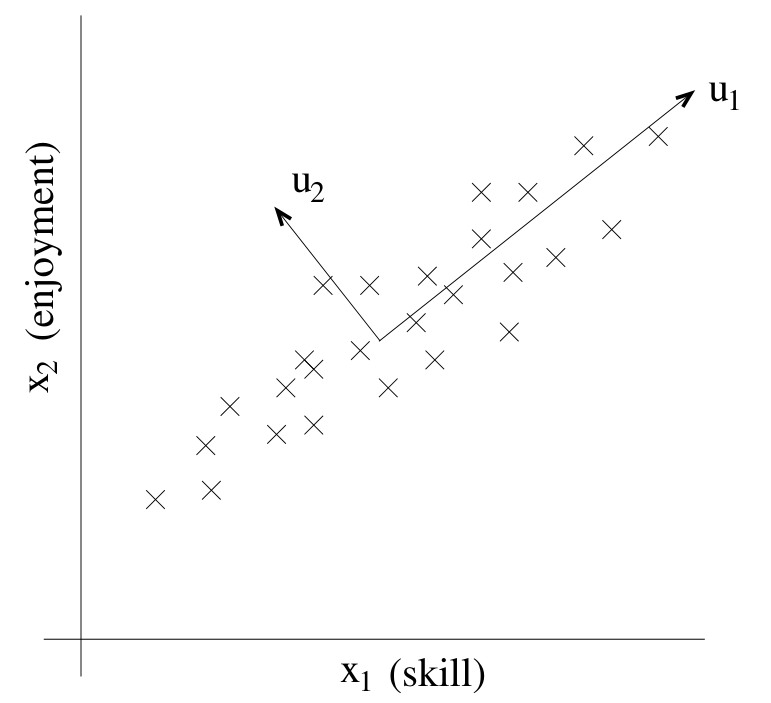
\includegraphics[width=0.6\textwidth]{figs/PCA.png}
\end{figure}

接下来将介绍 PCA 算法。但在正式运行 PCA 之前,通常首先通过归一化每个特征来预处理数据,使其均值为 0,方差为 1。具体做法是减去均值并除以经验标准差:
\[
    x_j^{(i)} \leftarrow \frac{x_j^{(i)} - \mu_j}{\sigma_j}
\]
其中 $\mu_j = \frac{1}{n} \sum_{i=1}^n x_j^{(i)}$ 和 $\sigma_j^2 = \frac{1}{n} \sum_{i=1}^n (x_j^{(i)} - \mu_j)^2$ 分别是特征 $j$ 的均值和方差。

减去 $\mu_j$ 会使均值变为零,对于已知均值为零的数据(例如,对应于语音或其他声学信号的时间序列)可以省略这一步。除以标准差 $\sigma_j$ 会将每个坐标重新缩放,使其具有单位方差,这确保了不同属性被视为同一“尺度”上的数据。例如,如果 $x_1$ 是汽车的最大速度(取值在几十到几百之间),而 $x_2$ 是座位数量(取值在 2-4 之间),那么这种重新归一化会重新缩放不同的属性,使它们更具可比性。如果已知不同属性都在同一尺度上,则可以省略这种缩放。一个例子是,如果每个数据点代表一个灰度图像,并且每个 $x_j^{(i)}$ 取值在 $\{0, 1, \dots, 255\}$ 之间,对应于图像 $i$ 中像素 $j$ 的强度值。

现在,数据已经归一化,如何计算“主要变化轴” $u$,即数据近似所在的那个方向?一种方法是将这个问题视为寻找单位向量 $u$,使得当数据被投影到对应于 $u$ 的方向上时,投影数据的方差最大化。直观地说,数据本身具有一定的方差/信息量。我们希望选择一个方向 $u$,使得如果我们将数据近似为位于对应于 $u$ 的方向/子空间中,则尽可能多地保留这些方差。

考虑以下已经归一化的数据集:

\begin{figure}[H]
    \centering
    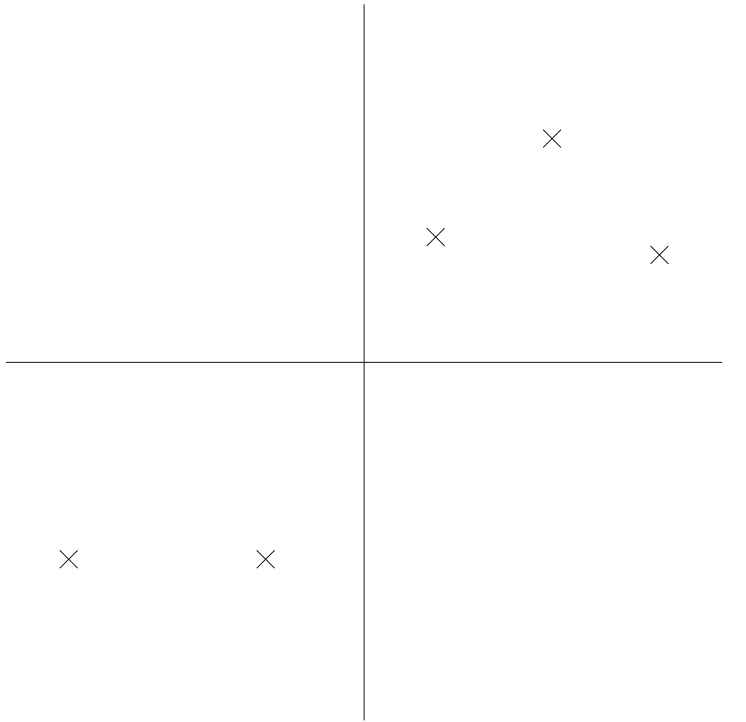
\includegraphics[width=0.6\textwidth]{figs/PCA_dataset.png}
\end{figure}

现在,假设选择的 $u$ 对应于下图所示的方向。圆圈表示原始数据点在该直线上的投影。

\begin{figure}[H]
    \centering
    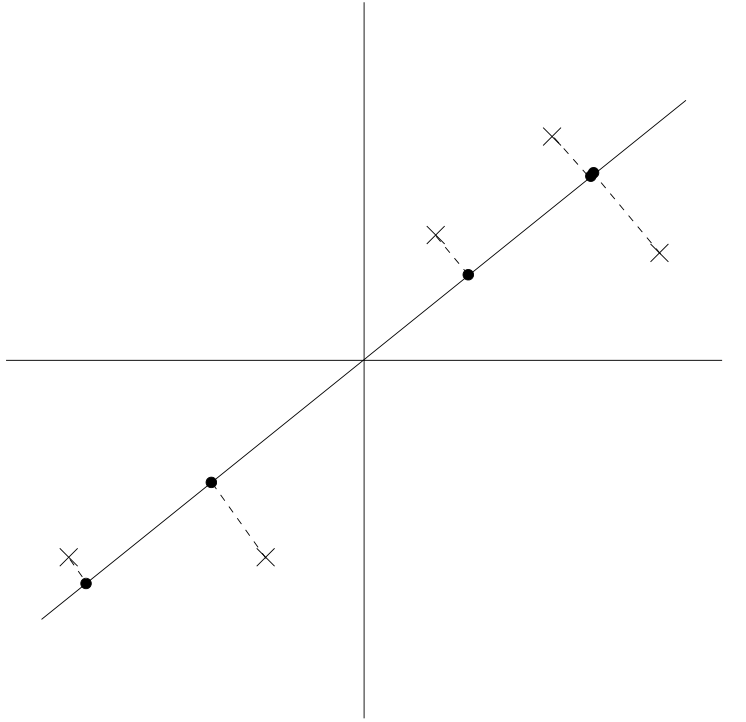
\includegraphics[width=0.6\textwidth]{figs/PCA_step1.png}
\end{figure}

可以看到,投影后的数据仍然具有相当大的方差,并且数据点倾向于远离零点。相比之下,如果选择以下方向:

\begin{figure}[H]
    \centering
    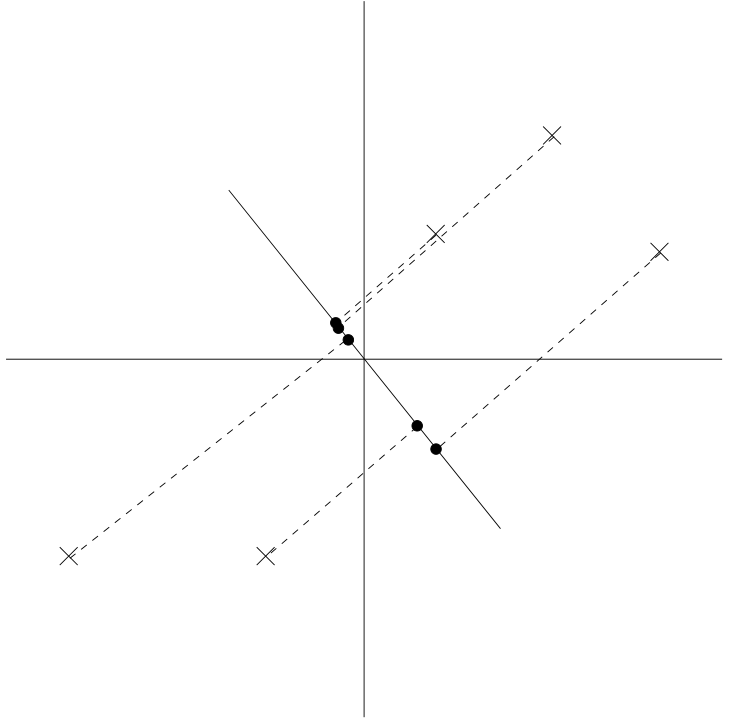
\includegraphics[width=0.6\textwidth]{figs/PCA_step2.png}
\end{figure}

在此方向上,投影的方差显著减小,并且更接近原点。

我们希望能够自动选择对应于上面所示两个图中的第一个图的方向 $u$。为了形式化这一点,请注意,给定一个单位向量 $u$ 和一个点 $x$, $x$ 在 $u$ 上的投影长度由 $x^T u$ 给出。也就是说,如果 $x^{(i)}$ 是数据集中的一个点(图中交叉点之一),那么它在 $u$ 上的投影(图中对应的圆圈)到原点的距离为 $x^{(i)T} u$。因此,为了最大化投影的方差,需要选择一个单位长度向量 $u$ 来最大化:
\begin{align*}
    \frac{1}{n} \sum_{i=1}^n (x^{(i)T} u)^2 
    &= \frac{1}{n} \sum_{i=1}^n u^T x^{(i)} x^{(i)T} u \\
    &= u^T \left( \frac{1}{n} \sum_{i=1}^n x^{(i)} x^{(i)T} \right) u.
\end{align*}
容易看出,在约束 $\|u\|_2 = 1$ 下最大化这个表达式会得到 $\Sigma = \frac{1}{n} \sum_{i=1}^n x^{(i)} x^{(i)T}$ 的主特征向量,这正是数据的经验协方差矩阵(假设数据均值为零)。\footnote{可以尝试使用拉格朗日乘子法来最大化 $u^T \Sigma u$,约束条件为 $u^T u = 1$。能够证明 $\Sigma u = \lambda u$ 对于某个 $\lambda$ 成立,这意味着 $u$ 是 $\Sigma$ 的特征向量,$\lambda$ 是对应的特征值。}

总而言之,如果希望找到一个一维子空间来近似数据,应该选择 $u$ 作为 $\Sigma$ 的主特征向量。更一般地,如果希望将数据投影到 $k$ 维子空间($k < d$),应该选择 $u_1, \dots, u_k$ 作为 $\Sigma$ 的前 $k$ 个特征向量。这些 $u_i$ 现在构成数据的一组新的正交基。\footnote{由于 $\Sigma$ 是对称的,所以 $u_i$ 是(或总是可以选择是)彼此正交的。}

然后,为了在该基下表示 $x^{(i)}$,只需要计算相应的向量
\[
    y^{(i)} = 
    \begin{bmatrix} 
        & u_1^T x^{(i)} & \\
        & u_2^T x^{(i)} & \\
        & \vdots & \\
        & u_k^T x^{(i)} & 
    \end{bmatrix} 
    \in \mathbb{R}^k.
\]
因此,尽管 $x^{(i)} \in \mathbb{R}^d$,我们能用向量 $y^{(i)}$ 作为 $x^{(i)}$ 的低维 $k$ 维近似/表示。PCA 也因此被称为一种\textbf{降维 (dimensionality reduction)} 算法。向量 $u_1, \dots, u_k$ 被称为数据的前 $k$ 个\textbf{主成分 (principal components)}。

\begin{remark*}
    尽管形式上只对 $k=1$ 的情况进行了推导,但利用特征向量的已知性质,很容易证明在所有可能的正交基 $u_1, \dots, u_k$ 中,我们选择的基最大化 $\sum_i \|y^{(i)}\|_2^2$。因此,我们选择的基保留了原始数据中尽可能多的变异性。
\end{remark*}


PCA 也可以通过选择最小化将数据投影到由基向量张成的 $k$ 维子空间所产生的近似误差的基来推导(详见习题集)。

PCA 有许多应用,下面将通过几个例子来结束讨论。首先,压缩——用较低维度的 $y^{(i)}$ 表示 $x^{(i)}$——是一个显而易见的应用。如果将高维数据降至 $k=2$ 或 3 维,那么还可以绘制 $y^{(i)}$ 来可视化数据。例如,如果将汽车数据降至 2 维,就可以绘制数据点(图中的一个点将对应一辆汽车,例如某种车型),从而了解哪些汽车彼此相似,以及哪些汽车群体可能聚类在一起。

另一个标准应用是在运行监督学习算法之前对数据集进行预处理,以降低其维度,将 $x^{(i)}$ 作为输入。除了计算上的好处外,降低数据的维度还可以降低所考虑的假设类的复杂度,并有助于避免过拟合(例如,低维输入空间上的线性分类器将具有较小的 VC 维)。

最后,在我们遥控直升机飞行员的例子中,也可以将 PCA 视为一种降噪算法。它估计了飞行技能和乐趣的内在“飞行业力”,而排除了嘈杂的测量结果。在课堂上,我们还看到了将这种思想应用于人脸图像的应用,产生了\textbf{特征脸 (eigenfaces)} 方法。在这里,每个点 $x^{(i)} \in \mathbb{R}^{100 \times 100}$ 是一个 10000 维向量,每个坐标对应于人脸图像中 100x100 像素的像素强度值。使用 PCA,我们将每个图像 $x^{(i)}$ 表示为一个低得多维度的 $y^{(i)}$。这样做,我们希望主成分能够保留人脸真正有趣、系统的变化,而不会保留由微小的光照变化、略微不同的成像条件等引入的图像中的“噪声”。然后,通过在降维空间中计算 $\|y^{(i)} - y^{(j)}\|_2$ 来测量人脸 $i$ 和 $j$ 之间的距离。这在人脸匹配和检索算法中取得了令人惊讶的好结果。

\chapter{独立成分分析 (ICA)}

\chapter{自监督学习与基础模型}
\part{强化学习与控制}

\chapter{强化学习}

现在开始学习强化学习和自适应控制。

监督学习中的算法试图使其输出模仿训练集中的标签 $y$。在这种设置下,对于每个输入 $x$,标签都给出了明确的“正确答案”。然而,对于许多序列决策和控制问题,很难为学习算法提供这种显式监督。例如,如果我们构建了一个四足机器人并试图对其进行编程以使其行走,那么我们其实不知道什么是使其行走的“正确”动作,因此也不知道如何为学习算法提供显式监督以供其模仿。

强化学习将转而为算法提供一个奖励函数,该函数指示学习智能体何时表现良好,何时表现不佳。在四足行走示例中,奖励函数可以对机器人向前移动给予正奖励,而对向后移动或摔倒给予负奖励。然后,学习算法的任务就是随着时间推移确定如何选择动作以获得高奖励。

强化学习已成功应用于各种领域,包括自主直升机飞行、机器人腿部运动、蜂窝网络路由、营销策略选择、工厂控制和高效网页索引。对强化学习的研究将从定义\textbf{马尔可夫决策过程 (Markov decision processess, MDP)} 开始,它提供了表述强化学习问题的一般化形式化框架。

\section{马尔可夫决策过程}

马尔可夫决策过程是一个元组 $(S, A, \{P_{s a}\}, \gamma, R)$,其中:
\begin{itemize}
    \item $S$ 是一个\textbf{状态 (states)} 集合。(例如,在自主直升机飞行中,$S$ 可以是直升机所有可能的位置和方向的集合。)
    \item $A$ 是一个\textbf{动作 (actions)} 集合。(例如,可以推动直升机控制杆的所有可能方向的集合。)
    \item $P_{sa}$ 是状态转移概率 (state transition probabilities)。对于每个状态 $s \in S$ 和动作 $a \in A$, $P_{sa}$ 是状态空间上的一个分布。稍后会详细介绍,但简而言之,$P_{sa}$ 给出了如果在状态 $s$ 采取动作 $a$ 后将转移到哪些状态的分布。
    \item $\gamma \in [0, 1]$ 称为\textbf{折扣因子 (discount factor)}。
    \item $R: S \times A \mapsto \mathbb{R}$ 是\textbf{奖励函数 (reward function)}。(奖励有时也写成仅关于状态 $S$ 的函数,在这种情况下有 $R: S \mapsto \mathbb{R}$)。
\end{itemize}
MDP 的动态过程如下:我们从某个状态 $s_0$ 开始,然后在 MDP 中选择一个动作 $a_0 \in A$ 执行。然后 MDP 的状态随机转移到某个后继状态 $s_1$,根据 $s_1 \sim P_{s_0 a_0}$ 抽取。然后选择另一个动作 $a_1$。由于这个动作,状态再次转移,现在转移到某个 $s_2 \sim P_{s_1 a_1}$,依此类推。可以将这个过程表示为:
\[
    s_0 \xrightarrow{a_0} s_1 \xrightarrow{a_1} s_2 \xrightarrow{a_2} s_3 \xrightarrow{a_3} \dots
\]

以动作序列 $a_0, a_1, \dots$ 遍历状态序列 $s_0, s_1, \dots$ 后,总收益由下式给出
\[
    R(s_0, a_0) + \gamma R(s_1, a_1) + \gamma^2 R(s_2, a_2) + \dots.
\]
或者,将奖励写成仅关于状态的函数时,则变为
\[
    R(s_0) + \gamma R(s_1) + \gamma^2 R(s_2) + \dots.
\]
在大部分推导中,将使用更简单的状态奖励 $R(s)$,尽管推广到状态-动作奖励 $R(s, a)$ 也不会有特别的困难。

在强化学习中,目标是随着时间推移选择动作以最大化总收益的期望值:
\[
    \text{E}\left[R(s_0) + \gamma R(s_1) + \gamma^2 R(s_2) + \dots\right]
\]
注意,时间步 $t$ 的奖励被 $\gamma^t$ \textbf{折扣 (discount)}。因此,为了使这个期望值最大化,希望尽快累积正奖励(并尽可能推迟负奖励)。在经济应用中,如果 $R(\cdot)$ 代表赚取的金额,那么 $\gamma$ 也有一个自然的利率解释(今天的一美元比明天的一美元更值钱)。

\textbf{策略 (policy)} 是一个函数 $\pi: S \mapsto A$,它将状态映射到动作。当处于状态 $s$ 时,如果\textbf{执行 (executing)} 某个策略 $\pi$,则采取动作 $a = \pi(s)$。同时定义策略 $\pi$ 的\textbf{价值函数 (value function)} 为
\[
    V^\pi(s) = \text{E}\left[R(s_0) + \gamma R(s_1) + \gamma^2 R(s_2) + \dots \mid s_0 = s, \pi\right].
\]
$V^\pi(s)$ 表示从状态 $s$ 开始并按照策略 $\pi$ 采取动作所获得的折扣奖励的期望总和。\footnote{请注意,这里以 $\pi$ 为条件的写法并不完全正确,因为 $\pi$ 不是随机变量,但这在文献中是相当标准的用法。}

给定一个固定的策略 $\pi$,其价值函数 $V^\pi$ 满足\textbf{贝尔曼方程 (Bellman equation)}:
\[
    V^\pi(s) = R(s) + \gamma \sum_{s' \in S} P_{s\pi(s)}(s') V^\pi(s').
\]
这表明从状态 $s$ 开始的折扣奖励期望总和 $V^\pi(s)$ 由两部分组成:第一部分是从状态 $s$ 开始即刻获得的\textbf{即时奖励 (immediate reward)} $R(s)$;第二部分是未来折扣奖励的期望总和。仔细考察第二项,可以看到上面的求和项可以重写为 $\text{E}_{s' \sim P_{s\pi(s)}}[V^\pi(s')]$。这是从状态 $s'$ 开始的折扣奖励的期望总和,其中 $s'$ 的分布由 $P_{s\pi(s)}$ 给出,也就是在 MDP 中从状态 $s$ 执行第一个动作 $\pi(s)$ 后将到达的状态分布。因此,上面的第二项给出的是在 MDP 中执行第一步后获得的折扣奖励的期望总和。

贝尔曼方程可以有效地用于求解 $V^\pi$。具体来说,在一个有限状态 MDP ($|S| < \infty$) 中,可以为每个状态 $s$ 写出一个关于 $V^\pi(s)$ 的方程。这给出了 $|S|$ 个线性方程组,其中包含 $|S|$ 个变量(未知的 $V^\pi(s)$),可以有效地求解这些变量。

同样地,定义\textbf{最优价值函数 (optimal value function)} 为
\begin{equation}
    V^*(s) = \max_{\pi} V^\pi(s).
    \label{eq:15.1}
\end{equation}
换句话说,这是使用任何策略可以达到的最佳期望折扣奖励总和。对于最优价值函数,也有一个贝尔曼方程:
\begin{equation}
    V^*(s) = R(s) + \max_{a \in A} \gamma \sum_{s' \in S} P_{sa}(s') V^*(s').
    \label{eq:15.2}
\end{equation}
上面的第一项是即时奖励。第二项是在执行动作 $a$ 之后获得的期望未来折扣奖励总和在所有动作 $a$ 上的最大值。应该确保理解这个方程及其合理性。

同时定义策略 $\pi^*: S \mapsto A$ 如下:
\begin{equation}
    \pi^*(s) = \arg \max_{a \in A} \sum_{s' \in S} P_{sa}(s') V^*(s').
    \label{eq:15.3}
\end{equation}
注意,$\pi^*(s)$ 给出了在方程\eqref{eq:15.2}中的 "max" 中达到最大值的动作 $a$。

事实证明,对于每一个状态 $s$ 和每一个策略 $\pi$,有
\[
    V^*(s) = V^{\pi^*}(s) \ge V^\pi(s).
\]
第一个等号表示,对于每个状态 $s$,策略 $\pi^*$ 的价值函数 $V^{\pi^*}$ 都等于最优价值函数 $V^*$。此外,不等号表示 $\pi^*$ 的价值至少与任何其他策略的价值一样大。换句话说,方程 \eqref{eq:15.3} 所定义的 $\pi^*$ 是\textbf{最优策略 (optimal policy)}。

注意,$\pi^*$ 具有一个有趣的性质,即它是\textit{所有 (all)} 状态 $s$ 的最优策略。也就是说,不会是这样:从某个状态 $s$ 开始的最优策略,与从另一个状态 $s'$ 开始的最优策略不同。同一个策略 $\pi^*$ 在\textit{所有 (all)} 状态 $s$ 下都达到了方程 \eqref{eq:15.1} 的最大值。这意味着无论 MDP 的初始状态是什么,都可以使用相同的策略 $\pi^*$。

\section{价值迭代与策略迭代}\label{sec:15.2}

现在介绍两种求解有限状态 MDP 的高效算法。目前,只考虑具有有限状态空间和动作空间(即 $|S| < \infty, |A| < \infty$)的 MDP。在本节中,还假设已知状态转移概率 $\{P_{sa}\}$ 和奖励函数 $R$。

第一个算法是\textbf{价值迭代 (value iteration)},如下所示:

\vspace{0.5em}
\begin{algorithm}[H]
    \SetAlgoNoLine
    \label{algo:4}
    \caption{价值迭代}
    对于每个状态 $s$,初始化 $V(s) := 0$。\\
    \For{直到收敛}{
        对于每个状态,更新
        \begin{equation}\label{eq:15.4}
            V(s) := R(s) + \max_{a \in A} \gamma \sum_{s'} P_{sa}(s') V(s').
        \end{equation}
    }
\end{algorithm}

这个算法可以看作是重复使用贝尔曼方程\eqref{eq:15.2}来更新估计的价值函数。

算法的内循环中更新 $V(s)$ 的方式有两种方式。第一种是先计算每个状态 $s$ 的新 $V(s)$ 值,然后用新值覆盖所有旧值。这称为\textbf{同步 (synchronous)} 更新。在这种情况下,算法可以看作是实现了一个“贝尔曼备份算子”,它接收价值函数的当前估计,并将其映射到一个新的估计。(详请参阅习题集。)另一种方法是执行\textbf{异步 (asynchronous)} 更新。在这种情况下,可以按某种顺序逐个状态进行循环,每次更新一个值。

在同步或异步更新下,可以证明价值迭代会使 $V$ 收敛到 $V^*$。找到 $V^*$ 后,可以使用方程\eqref{eq:15.3}来找到最优策略。

除了价值迭代,还有另一种算法用于寻找 MDP 的最优策略。\textbf{策略迭代 (policy iteration)} 算法如下:

\vspace{0.5em}
\begin{algorithm}[H]
    \SetKwComment{Comment}{$\triangleright$\ }{}
    \SetAlgoNoLine
    \label{algo:5}
    \caption{策略迭代}
    随机初始化 $\pi$。\\
    \For{直到收敛}{
        令 $V := V^\pi.$ \Comment*[f]{通常用线性系统求解器处理}\\
        对于每个状态 $s$,令
        \begin{equation*}
            \pi(s) := \arg\max_{a \in A} \sum_{s'}P_{s a}(s')V(s').
        \end{equation*}
    }
\end{algorithm}

因此,内循环重复计算当前策略的价值函数,然后使用当前价值函数更新策略。(步骤 (b) 中找到的策略也称为关于 $V$ 的\textbf{贪婪策略 (greedy policy)}。)注意,步骤 (a) 可以通过求解贝尔曼方程来实现,如前所述,对于一个固定的策略,这仅仅是关于 $|S|$ 个变量的 $|S|$ 个线性方程组。
经过该算法的\textit{有限 (finite)} 次迭代后,$V$ 将收敛到 $V^*$,并且 $\pi$ 将收敛到 $\pi^*$。\footnote{注意,价值迭代无法在有限次迭代中达到精确的 $V^*$,但策略迭代可以使用精确的线性方程组求解器,因此可以精确收敛。这是因为当动作空间和策略空间是离散且有限时,一旦策略迭代中的策略达到最优策略,它将不再改变。另一方面,尽管价值迭代会收敛到 $V^*$,但学习到的价值函数中总是存在一些非零误差。}

价值迭代和策略迭代都是求解 MDP 的标准算法,目前对于哪种算法更好还没有普遍共识。对于小型 MDP,策略迭代通常非常快,并且在很少的迭代次数内收敛。然而,对于状态空间较大的 MDP,显式求解 $V^*$ 将涉及求解一个大型线性方程组,这可能会很困难(并且注意在策略迭代中需要多次求解线性方程组)。在这些问题中,价值迭代可能更受欢迎。因此,在实践中,价值迭代似乎比策略迭代更常用。关于价值迭代和策略迭代的比较和联系的更多讨论,请参阅第 \ref{sec:15.5} 节。

\section{学习 MDP 的模型}

到目前为止,所讨论的 MDP 和求解 MDP 的算法都假设已知状态转移概率和奖励。在许多现实问题中,我们无法直接获得状态转移概率和奖励,而是必须从数据中估计它们。(通常,状态空间 $S$、动作空间 $A$ 和折扣因子 $\gamma$ 是已知的。)例如,假设对于倒立摆问题(参见习题集 4),我们在 MDP 中进行了一些试验,过程如下:
\begin{align*}
    &s_0^{(1)} \xrightarrow{a_0^{(1)}} s_1^{(1)} \xrightarrow{a_1^{(1)}} s_2^{(1)} \xrightarrow{a_2^{(1)}} s_3^{(1)} \xrightarrow{a_3^{(1)}} \dots \\
    &s_0^{(2)} \xrightarrow{a_0^{(2)}} s_1^{(2)} \xrightarrow{a_1^{(2)}} s_2^{(2)} \xrightarrow{a_2^{(2)}} s_3^{(2)} \xrightarrow{a_3^{(2)}} \dots\\
    &\cdots
\end{align*}
这里,$s_i^{(j)}$ 是在第 $j$ 次试验的时刻 $i$ 时的状态,$a_i^{(j)}$ 是在该状态下采取的相应动作。在实践中,上述每一次试验可能会持续到 MDP 终止(例如,倒立摆问题中,摆杆倒下),或者可能运行很长但有限的时间步。

给定由多次试验组成的 MDP 中的这种“经验”,可以很容易地得出状态转移概率的最大似然估计:
\begin{equation}
    P_{sa}(s') = \frac{\text{在状态 $s$ 采取动作 $a$ 到达状态 $s'$ 的次数}}{\text{在状态 $s$ 采取动作 $a$ 的次数}}
    \label{eq:15.5}
\end{equation}
或者,如果上述比率是“0/0”——对应于之前从未在状态 $s$ 采取动作 $a$ 的情况——我们可以简单地将 $P_{sa}(s')$ 估计为 $1/|S|$。(即,将 $P_{sa}$ 估计为关于所有状态的均匀分布。)

注意,如果得到了更多经验(观察了更多试验),有一种有效的方法可以使用新的经验更新状态转移概率估计。具体来说,如果我们跟踪 \eqref{eq:15.5} 中分子和分母的计数,那么当观察更多试验时,可以简单地累加这些计数。计算这些计数的比率即可得到对 $P_{sa}$ 的估计。

使用类似的过程,如果 $R$ 未知,也可以将状态 $s$ 中预期即时奖励 $R(s)$ 的估计值取为在状态 $s$ 中观察到的平均奖励。

在学习了 MDP 的模型后,可以使用价值迭代或策略迭代来求解 MDP,使用估计的状态转移概率和奖励。例如,将模型学习和价值迭代结合起来,是学习具有未知状态转移概率的 MDP 的一种可能的算法:

\begin{enumerate}
    \item 随机初始化 $\pi$。
    \item 重复 \{
        \begin{enumerate}
            \item 在 MDP 中执行一定次数的 $\pi$,收集经验。
            \item 使用上述经验更新状态转移概率 $P_{sa}$ 的估计值(如果可行的话,也更新 $R$ 的估计值)。
            \item 根据估计的状态转移概率和奖励,使用价值迭代更新价值函数 $V$ 的估计值。
            \item 更新策略 $\pi$,使其成为关于 $V$ 的贪婪策略。
        \end{enumerate}
    \}
\end{enumerate}

注意到,对于该算法,有一个简单的优化可以使其运行得更快。具体来说,在算法的内层循环中,应用价值迭代时,如果不是将价值迭代初始化为 $V=0$,而是用算法前一次迭代中找到的解进行初始化,那么这将为价值迭代提供一个更好的起始点,并使其更快收敛。

\section{连续状态 MDP}

之前我们主要关注了有限状态数量的 MDP。现在我们将讨论可能具有无限状态数量的 MDP 的算法。例如,对于汽车,我们可以将状态表示为 $(x, y, \theta, \dot{x}, \dot{y}, \dot{\theta})$,其中包括其位置 $(x, y)$;方向 $\theta$;在 $x$ 和 $y$ 方向上的速度 $\dot{x}$ 和 $\dot{y}$;以及角速度 $\dot{\theta}$。因此,$S = \mathbb{R}^6$ 是一个无限状态集,因为汽车有无限多的可能位置和方向。\footnote{严格来说,$\theta$ 是一个方向,因此 $\theta$ 的范围写成 $\theta \in [-\pi, \pi)$ 比 $\theta \in \mathbb{R}$ 更合适;但对我们的目标而言,这种区别并不重要。} 类似地,在习题集 4 中的倒立摆具有状态 $(x, \theta, \dot{x}, \dot{\theta})$,其中 $\theta$ 是摆杆的角度。而一架在 3D 空间中飞行的直升机具有 $(x, y, z, \phi, \theta, \psi, \dot{x}, \dot{y}, \dot{z}, \dot{\phi}, \dot{\theta}, \dot{\psi})$ 形式的状态,其中横滚角 $\phi$、俯仰角 $\theta$ 和偏航角 $\psi$ 指定了直升机的 3D 方向。

在本节中,我们将考虑状态空间为 $S = \mathbb{R}^d$ 的情况,并描述解决此类 MDP 的方法。

\subsection{离散化}

解决连续状态 MDP 的最简单方法可能是离散化状态空间,然后使用之前描述的价值迭代或策略迭代等算法。

例如,对于 2D 状态 $(s_1, s_2)$,可以使用网格来离散化状态空间:

\begin{figure}[H]
    \centering
    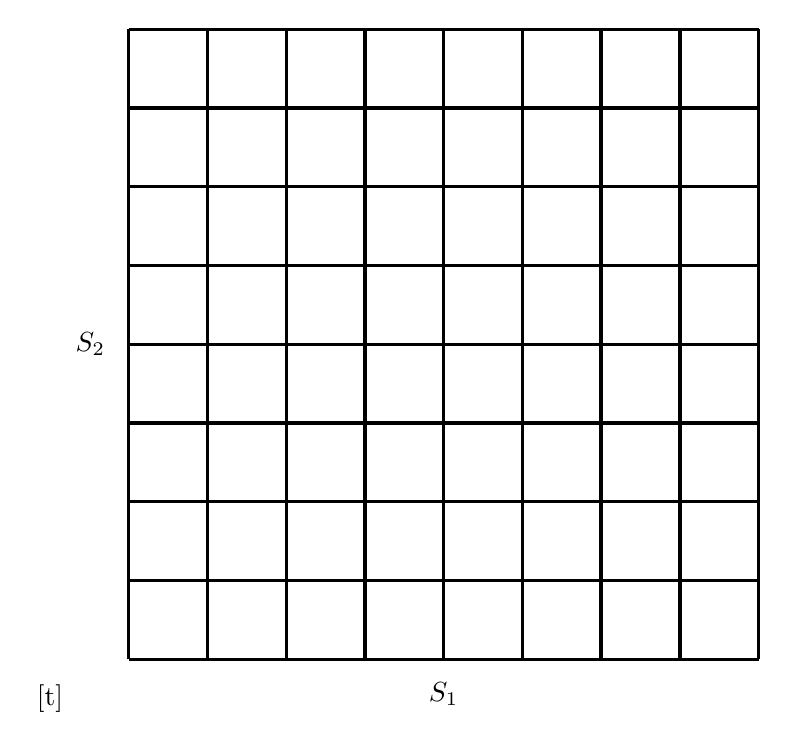
\begin{tikzpicture}
        \def\gridsize{8}
        \draw[step=1, very thick, black] (0,0) grid (\gridsize, \gridsize);
        \node[below=5pt] at (\gridsize/2, 0) {$S_1$};
        \node[left=5pt] at (0, \gridsize/2) {$S_2$};
        \node at (-1, -0.5) {[t]};
    \end{tikzpicture}
\end{figure}

这里,每个网格单元代表一个独立的离散状态 $\bar{s}$。然后,可以通过一个离散状态 MDP $(\bar{S}, A, \{P_{\bar{s}a}\}, \gamma, R)$ 来近似连续状态 MDP,其中 $\bar{S}$ 是离散状态的集合,$\{P_{\bar{s}a}\}$ 是离散状态上的状态转移概率。然后,可以使用价值迭代或策略迭代来解出离散状态 MDP $(\bar{S}, A, \{P_{\bar{s}a}\}, \gamma, R)$ 中的 $V^*(\bar{s})$ 和 $\pi^*(\bar{s})$。当实际系统处于某个连续值状态 $s \in S$ 并且需要选择一个动作来执行时,就计算相应的离散化状态 $\bar{s}$,并执行动作 $\pi^*(\bar{s})$。

这种离散化方法对于许多问题都能很好地工作。然而,它有两个缺点。首先,它对 $V^*$(以及 $\pi^*$)使用了相当简单的表示。具体来说,它假设价值函数在每个离散化区间上取一个常数值(即,价值函数在每个网格单元中是分段常数)。

为了更好地理解这种表示的局限性,考虑一个\textit{监督学习 (supervised learning)} 问题,将函数拟合到这个数据集:

\begin{figure}[H]
    \centering
    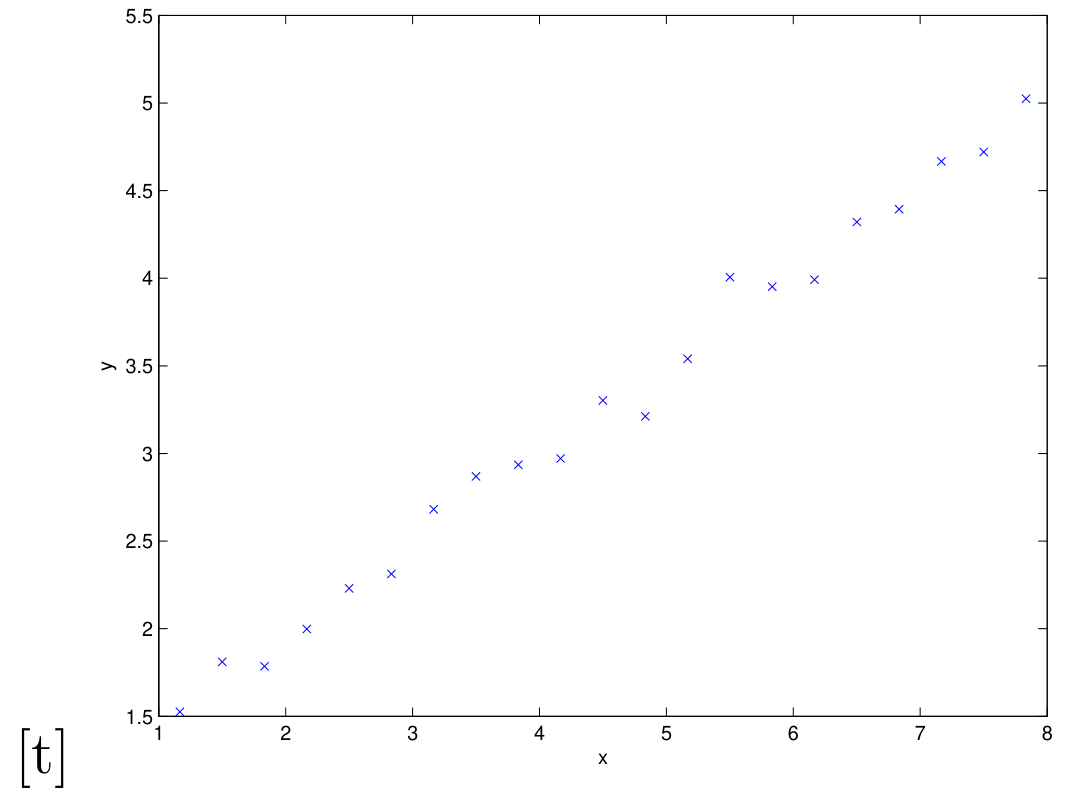
\includegraphics[width=0.6\textwidth]{figs/rl_dataset.png}
\end{figure}

显然,线性回归可以很好地拟合这个数据集,然而,如果对 x 轴离散化,并使用在每个离散区间内为分段常数的表示,那么我们对数据的拟合将如下所示:

\begin{figure}[H]
    \centering
    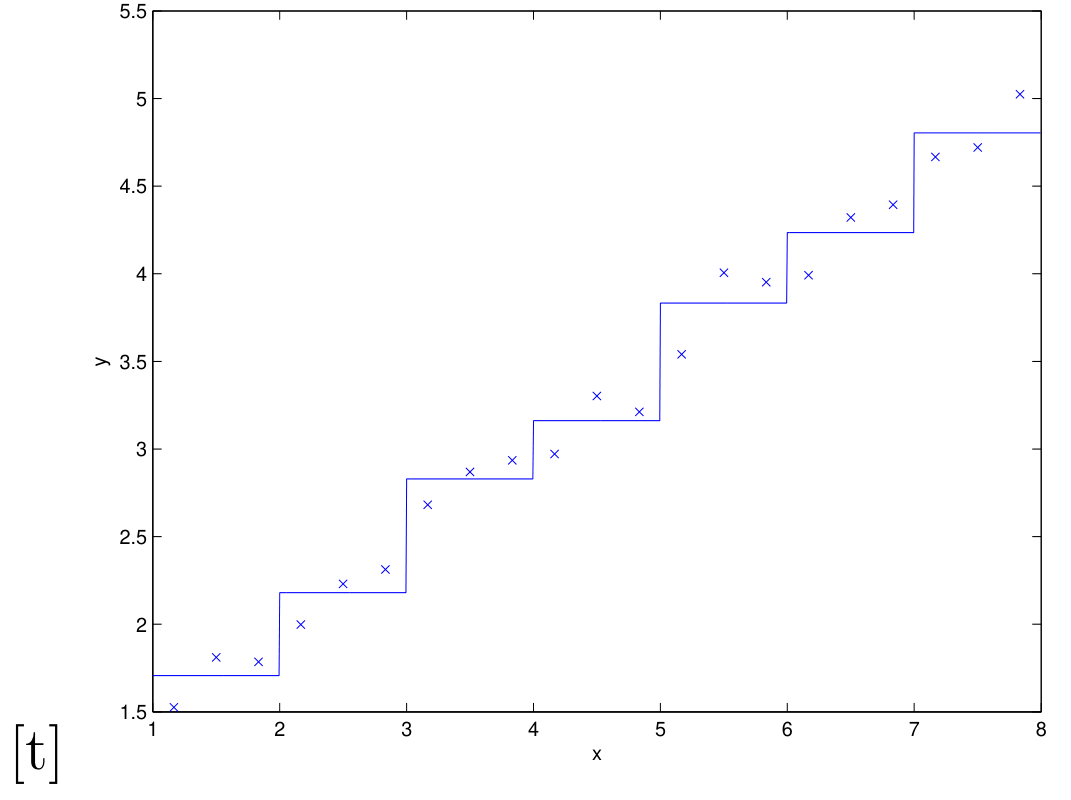
\includegraphics[width=0.6\textwidth]{figs/rl_dataset_discrete.png}
\end{figure}

这种分段常数表示对于许多平滑函数来说并不是一个好的表示。它导致输入上的平滑性很差,并且在不同网格单元之间没有泛化能力。使用这种表示,我们需要非常精细的离散化(非常小的网格单元)才能获得良好的近似。

这种表示的第二个缺点被称为\textbf{维度诅咒 (curse of dimensionality)}。假设 $S = \mathbb{R}^d$,并且我们将状态的 $d$ 个维度中的每一个都离散化为 $k$ 个值。那么我们拥有的离散状态总数为 $k^d$。这在状态空间维度 $d$ 中呈指数级增长,因此不适用于大型问题。例如,对于一个 10 维状态,如果我们将每个状态变量离散化为 100 个值,我们将有 $100^{10} = 10^{20}$ 个离散状态,这对于现代计算机来说也大到无法表示。

根据经验,离散化通常对于 1 维和 2 维问题非常有效(而且简单且快速实现)。也许用一些取巧的办法,并在选择离散化方法时谨慎一些,它也能适用于 4 维状态的问题。如果你非常聪明且幸运,甚至可能让它适用于某些 6 维问题。但它很少适用于更高维度的问题。

\subsection{价值函数近似}

我们现在介绍一种在连续状态 MDP 中寻找策略的替代方法,即直接近似 $V^*$,而无需诉诸离散化。这种方法被称为价值函数近似,且已成功应用于许多强化学习问题。

\subsubsection*{使用模型或模拟器}

为了开发值函数近似算法,我们将假设我们拥有一个用于 MDP 的\textbf{模型 (model)} 或\textbf{模拟器 (simulator)}。非正式地,模拟器是一个黑盒,它接收任何(连续值)状态 $s_t$ 和动作 $a_t$ 作为输入,并根据状态转移概率 $P_{s_t a_t}$ 输出下一个状态 $s_{t+1}$ 的采样。

\begin{figure}[H]
    \centering
    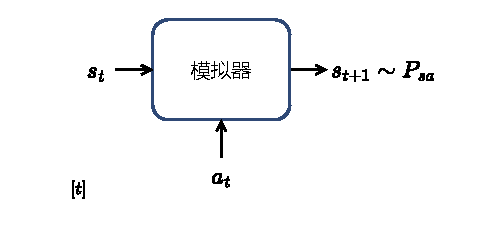
\includegraphics[width=0.5\textwidth]{figs/simulator.pdf}
\end{figure}

获取此类模型有多种方法。一种是使用物理模拟。例如,习题集 4 中倒立摆的模拟器是通过使用物理定律计算在给定当前状态 $t$ 和所采取的动作 $a$ 的情况下,小车/杆在时间 $t+1$ 的位置和方向来获得的,前提是已知系统的所有参数,例如杆的长度、杆的质量等。或者,也可以使用现成的物理模拟软件包,该软件包将机械系统的完整物理描述、当前状态 $s_t$ 和动作 $a_t$ 作为输入,并在未来一小段时间内计算出系统的状态 $s_{t+1}$。\footnote{Open Dynamics Engine (\url{http://www.ode.com}) 是一个免费/开源的物理模拟器示例,可用于模拟倒立摆等系统,并且在强化学习研究人员中一直是一个受欢迎的选择。}

获取模型的另一种方法是从 MDP 中收集的数据中学习一个模型。例如,假设执行 $n$ 次\textbf{试验 (trials)},每次试验重复在 MDP 中采取动作,且持续 $T$ 个时间步。可以随机选择动作、执行某些特定策略或通过其他方式选择动作。然后,将观察到 $n$ 个状态序列,如下所示:
\begin{align*}
    &s_0^{(1)} \xrightarrow{a_0^{(1)}} s_1^{(1)} \xrightarrow{a_1^{(1)}} s_2^{(1)} \xrightarrow{a_2^{(1)}} \dots \xrightarrow{a_{T-1}^{(1)}} s_T^{(1)} \\
    &s_0^{(2)} \xrightarrow{a_0^{(2)}} s_1^{(2)} \xrightarrow{a_1^{(2)}} s_2^{(2)} \xrightarrow{a_2^{(2)}} \dots \xrightarrow{a_{T-1}^{(2)}} s_T^{(2)} \\
    &\dots \\
    &s_0^{(n)} \xrightarrow{a_0^{(n)}} s_1^{(n)} \xrightarrow{a_1^{(n)}} s_2^{(n)} \xrightarrow{a_2^{(n)}} \dots \xrightarrow{a_{T-1}^{(n)}} s_T^{(n)}
\end{align*}
然后,可以应用学习算法来预测 $s_{t+1}$ 作为 $s_t$ 和 $a_t$ 的函数。

例如,可以选择学习一个如下形式的线性模型:
\begin{equation}
    s_{t+1} = As_t + Ba_t,
    \label{eq:15.6}
\end{equation}
使用类似于线性回归的算法。这里,模型的参数是矩阵 $A$ 和 $B$,并且可以通过从 $n$ 次试验中收集的数据来估计它们:
\[
    \underset{A,B}{\arg \min} \sum_{i=1}^n \sum_{t=0}^{T-1} \left\| s_{t+1}^{(i)} - (As_t^{(i)} + Ba_t^{(i)}) \right\|^2.
\]

也可以使用其他损失函数来学习模型。例如,最近 \cite{luo2018algorithmic} 的工作发现,使用 $\left\| \cdot \right\|_2$ 范数(不带平方)在某些情况下可能有所帮助。

在学习了 $A$ 和 $B$ 之后,一个选项是构建一个\textbf{确定性 (deterministic)} 模型,其中给定输入 $s_t$ 和 $a_t$,输出 $s_{t+1}$ 被精确确定。具体来说,总是根据公式 \eqref{eq:15.6} 计算 $s_{t+1}$。或者,也可以构建一个\textbf{随机 (stochastic)} 模型,其中 $s_{t+1}$ 是输入的随机函数,通过将其建模为:
\[
    s_{t+1} = As_t + Ba_t + \epsilon_t,
\]
其中 $\epsilon_t$ 是一个噪声项,通常建模为 $\epsilon_t \sim \mathcal{N}(0, \Sigma)$。(协方差矩阵 $\Sigma$ 也可以以直接的方式从数据中估计。)

这里将下一个状态 $s_{t+1}$ 写成当前状态和动作的线性函数;当然,这也可以是非线性函数。具体来说,可以学习一个模型 $s_{t+1} = A\phi_s(s_t) + B\phi_a(a_t)$,其中 $\phi_s$ 和 $\phi_a$ 是状态和动作的一些非线性特征映射。或者,也可以使用非线性学习算法,例如局部加权线性回归,来估计 $s_{t+1}$ 作为 $s_t$ 和 $a_t$ 的函数。这些方法都可以用来构建 MDP 的确定性或随机模拟器。

\subsubsection*{拟合价值迭代}

现在介绍用于近似连续状态 MDP 价值函数的\textbf{拟合价值迭代 (fitted value iteration)} 算法。在下文中,我们将假设问题具有连续状态空间 $S = \mathbb{R}^d$,但动作空间 $A$ 较小且离散。\footnote{在实践中,大多数 MDP 的动作空间远小于状态空间。例如,汽车状态空间有 6 维而动作空间则是 2 维(转向和速度控制);倒立摆状态空间有 4 维而动作空间只有 1 维;直升机则是 12 维状态空间和 4 维动作空间。因此,离散化动作空间通常比离散化状态空间的问题要小得多。}

回顾一下,价值迭代执行以下更新:
\begin{align}
    V(s) &:= R(s) + \gamma \max_a \int_{s'} P_{sa}(s')V(s')ds' \label{eq:15.7} \\
    &= R(s) + \gamma \max_a \mathrm{E}_{s' \sim P_{sa}} [V(s')] \label{eq:15.8}
\end{align}
(在第 \ref{sec:15.2} 节中,价值迭代更新写为 $V(s) := R(s) + \gamma \max_a \sum_{s'} P_{sa}(s')V(s')$ 而不是状态上的积分;新的符号反映了现在正在处理连续状态而不是离散状态。)

拟合价值迭代的主要思想是,在有限样本状态 $s^{(1)}, \dots, s^{(n)}$ 上近似地执行此步骤。具体来说,下面使用监督学习算法——线性回归——来近似状态的价值函数,作为状态的线性或非线性函数:
\[
    V(s) = \theta^T \phi(s).
\]
这里,$\phi$ 是状态的某种适当的特征映射。

对于具有的有限样本 $n$ 个状态中的每个状态 $s$,拟合价值迭代将首先计算一个量 $y^{(i)}$,是 $R(s) + \gamma \max_a \mathrm{E}_{s' \sim P_{sa}} [V(s')]$ 的近似(公式 \eqref{eq:15.8} 的右侧)。然后将应用监督学习算法,尝试使 $V(s)$ 接近 $R(s) + \gamma \max_a \mathrm{E}_{s' \sim P_{sa}} [V(s')]$(换句话说,尝试使 $V(s)$ 接近 $y^{(i)}$)。

详细来说,该算法如下:
\begin{enumerate}
    \item 随机采样 $n$ 个状态 $s^{(1)}, s^{(2)}, \cdots, s^{(n)} \in S$。
    \item 初始化 $\theta := 0$。
    \item 重复 \{
        \begin{itemize}
            \item[] 对于 $i = 1, \dots, n$ \{
                \begin{itemize}
                    \item[] 对于每个动作 $a \in A$ \{
                        \begin{itemize}
                            \item[] 采样 $s_1', \cdots, s_k' \sim P_{s^{(i)} a}$(使用某种 MDP 模型)。
                            \item[] 令 $q(a)=\frac1k \sum_{j=1}^{k} R(s^{(i)}) + \gamma V(s_j')$。
                            \item[] \qquad // 因此,$q(a)$ 是 $R(s^{i}) + \gamma \mathrm{E}_{s'\sim P_{s^{(i) a}}}[V(s')]$ 的估计值。
                        \end{itemize}

                    \}
                    \item[] 令 $y^{(i)} = \max_a q(a)$。
                    \item[] \qquad // 因此, $y^{(i)}$ 是 $R(s^{i}) + \gamma \max_a \mathrm{E}_{s'\sim P_{s^{(i) a}}}[V(s')]$ 的估计值。
                \end{itemize}
            \}
            \item[] // 原始的(用于离散状态的)价值迭代算法
            \item[] // 根据 $V(s^{(i)}) := y^{(i)}$ 更新价值函数。
            \item[] // 此算法则希望 $V(s^{(i)}) \approx y^{(i)}$
            \item[] // 可以使用监督学习(线性回归)达成这点。
            \item[] 令 $\theta := \arg\min_\theta \frac12 \sum_{i=1}^{n} \left(\theta^T \phi(s^{(i)}) - y^{(i)}\right)^2$。
        \end{itemize}
        
    \}
\end{enumerate}

如上所述,我们已经详细阐述了使用线性回归的拟合价值迭代算法,以使 $V(s^{(i)})$ 接近 $y^{(i)}$。算法的这一步骤完全类似于标准的监督学习(回归)问题,其中有一个训练集 $(x^{(1)}, y^{(1)}), (x^{(2)}, y^{(2)}), \dots, (x^{(n)}, y^{(n)})$,并且希望学习一个从 $x$ 到 $y$ 的函数;唯一的区别是这里 $s$ 扮演了 $x$ 的角色。尽管上面的描述使用了线性回归,但显然也可以使用其他回归算法(例如局部加权线性回归)。

与离散状态集上的价值迭代不同,拟合价值迭代不能被证明总是收敛的。然而,它在实践中通常能收敛(或近似收敛),并且对许多问题都表现良好。还需要注意的是,如果使用 MDP 的确定性模拟器/模型,那么可以通过在算法中设置 $k=1$ 来简化拟合价值迭代。这是因为公式 \eqref{eq:15.8} 中的期望变为确定性分布上的期望,因此一个单一的样本就足以精确计算该期望。否则,在上述算法中,需要抽取 $k$ 个样本并取平均值来近似该期望(参见算法伪代码中 $q(a)$ 的定义)。

最后,拟合价值迭代输出 $V$ 作为 $V^*$ 的近似。这隐式地定义了我们的策略。具体来说,当系统处于某个状态 $s$,需要选择一个动作时,我们希望选择以下动作:
\begin{equation}
    \arg \max_a \mathrm{E}_{s' \sim P_{sa}} [V(s')] \label{eq:15.9}
\end{equation}
计算/近似此过程类似于拟合价值迭代的内循环,其中对于每个动作,我们从 $P_{sa}$ 中采样 $s'_1, \dots, s'_k$ 来近似期望。(同样,如果模拟器是确定性的,我们可以设置 $k=1$。)

在实践中,通常还有其他方法来近似此步骤。例如,一个非常常见的情况是模拟器具有 $s_{t+1} = f(s_t, a_t) + \epsilon_t$ 的形式,其中 $f$ 是状态的某个确定性函数(例如 $f(s_t, a_t) = As_t + Ba_t$),$\epsilon_t$ 是零均值高斯噪声。在这种情况下,我们可以通过以下方式选择动作:
\[
    \arg \max_a V(f(s, a)).
\]
换句话说,这里是设置 $\epsilon_t = 0$(即,忽略模拟器中的噪声),并设置 $k=1$。等效地,这可以从公式 \eqref{eq:15.9} 使用以下近似导出:
\begin{align}
    \mathrm{E}_{s'}[V(s')] &\approx V(\mathrm{E}_{s'}[s']) \label{eq:15.10} \\
    &= V(f(s, a)), \label{eq:15.11}
\end{align}
其中期望是关于随机变量 $s' \sim P_{sa}$ 的。只要噪声项 $\epsilon_t$ 很小,这通常是一个合理的近似。

然而,对于那些不适合这种近似的问题,为了近似上述期望,需要使用模型对 $k|A|$ 个状态进行采样,这在计算上可能非常昂贵。

\section{策略与价值的联系 (选读)}\label{sec:15.5}

\vspace{0.5em}
\begin{algorithm}[H]
    \SetKwComment{Comment}{$\triangleright$\ }{}
    \SetAlgoNoLine
    \label{algo:6}
    \caption{策略迭代的变体}
    \textbf{过程} VE($\pi$, k) \Comment*[f]{用于评估 $V^\pi$}\\
    \quad 选项 1:初始化 $V := 0$;选项 2:使用主算法的当前 $V$ 进行初始化。\\
    \quad \For{$i=0$ \KwTo $k-1$}{
        \quad 对于每个状态 $s$,更新
        \begin{equation}
            V(s) := R(s) + \gamma \sum_{s'} P_{s \pi(s)}(s')V(s').\label{eq:15.12}
        \end{equation}
    }
    \textbf{返回} $V$

    \ \\
    \textbf{输入}\ 超参数 $k$。\\
    随机初始化 $\pi$。\\
    \For{直到收敛}{
        令 $V := VE(\pi, k).$\\
        对于每个状态 $s$,令
        \begin{equation}
            \pi(s) := \arg\max_{a \in A} \sum_{s'}P_{s a}(s')V(s').\label{eq:15.13}
        \end{equation}
    }
\end{algorithm}

在策略迭代算法 \ref{algo:5} 的第 3 行,通常用线性系统求解器来计算 $V^\pi$。或者也可以使用迭代贝尔曼更新来评估 $V^\pi$,这类似于价值迭代,如算法 \ref{algo:6} 中过程 VE($\cdot$) 的第 1 行所示。如果我们在过程 VE 的第 2 行中选择选项 1,那么过程 VE 与价值迭代(算法 \ref{algo:4})的不同之处在其第 4 行:过程 VE 用 $\pi$ 中的动作,而价值迭代则使用贪婪动作。

用过程 VE 可以构建算法 \ref{algo:6},它是策略迭代的一种变体,作为连接策略迭代和价值迭代的中间算法。这里我们在 VE 中选用选项 2,以最大化重用之前所学的知识。可以验证,如果取 $k=1$ 并在算法 \ref{algo:6} 的第 2 行中选用选项 2,那么算法 \ref{algo:6} 在语义上等同于价值迭代(算法 \ref{algo:4})。换句话说,算法 \ref{algo:6} 和价值迭代交错更新 \eqref{eq:15.13} 和 \eqref{eq:15.12}。算法 \ref{algo:6} 在更新 $k$ 步 \eqref{eq:15.12} 和一步 \eqref{eq:15.13} 之间交替,而价值迭代在更新一步 \eqref{eq:15.12} 和一步 \eqref{eq:15.13} 之间交替。因此,算法 \ref{algo:6} 通常不会比价值迭代更快,因为假设更新 \eqref{eq:15.12} 和 \eqref{eq:15.13} 效用和耗时相同,那么更新频率的最佳平衡可能只是 $k=1$ 或 $k \approx 1$。

另一方面,如果更新 $k$ 步 \eqref{eq:15.12} 可以比更新一步 \eqref{eq:15.12} $k$ 次快得多,那么多求几步 \eqref{eq:15.12} 可能有用。这就是策略迭代所利用的——线性系统求解器求解 $k=\infty$ 的 VE 比求解较大的 $k$ 的 VE 会快得多。反之,如果不存在这种加速效果,例如当状态空间很大且线性系统求解器也不快时,价值迭代更可取。

\chapter{LQR, DDP 与 LQG}

\section{有限时间范围的 MDP}\label{sec:16.1}

第15章中定义了马尔可夫决策过程,并讨论了简化设置下的价值迭代/策略迭代。具体而言,引入了定义最优策略 $\pi^*$ 的最优价值函数 $V^*$ 的\textbf{最优贝尔曼方程 (optimal Bellman equation)}。
\[
    V^*(s) = R(s) + \max_{a \in A}\gamma \sum_{s' \in S} P_{sa}(s')V^*(s')
\]

回想一下,从最优价值函数中能恢复最优策略$\pi^*$,如下所示:
\[
    \pi^*(s) = \operatorname*{argmax}_{a \in A} \sum_{s' \in S} P_{sa}(s')V^*(s')
\]

在本章中,将采用更一般的设置:
\begin{enumerate}
    \item 为了同时适用于离散和连续的情况。因此,将使用
    \begin{align*}
        &\mathbb{E}_{s' \sim P_{sa}}[V^{\pi^*}(s')] \quad \text{而非} \\
        &\sum_{s' \in S} P_{sa}(s')V^{\pi^*}
    \end{align*}
    这意味着将取下一状态价值函数的期望。在离散情况下,可以将期望改写为对所有状态的求和。在连续情况下,可以将期望改写为对所有状态的积分。符号 $s' \sim P_{sa}$ 表示 $s'$ 是从分布 $P_{sa}$ 中采样的。
    \item  假设奖励同时取决于\textbf{状态和动作 (both states and actions)}。换句话说,$R: \mathcal{S} \times \mathcal{A} \to \mathbb{R}$。这意味着计算最优动作的先前机制变为
    \[
        \pi^*(s) = \underset{a \in \mathcal{A}}{\text{argmax}} \ R(s, a) + \gamma \mathbb{E}_{s' \sim P_{sa}} [V^{\pi^*}(s')]
    \]
    \item 不考虑无限时间范围的 MDP,而是假设有一个\textbf{有限时间范围的 MDP (finite horizon MDP)},定义为一个元组
    \[
        (\mathcal{S}, \mathcal{A}, P_{sa}, T, R)
    \]
    其中 $T > 0$ 是\textbf{时间范围 (time horizon)}(例如 $T=100$)。在这种设置下,对回报的定义将略有不同:
    \[
        R(s_0, a_0) + R(s_1, a_1) + \cdots + R(s_T, a_T)
    \]
    而不是(无限时间范围情况下的)
    \begin{align*}
        & R(s_0, a_0) + \gamma R(s_1, a_1) + \gamma^2 R(s_2, a_2) + \cdots
        & \sum_{t=0}^{\infty} R(s_t, a_t)\gamma^t
    \end{align*}
    \textit{折现因子 $\gamma$ 呢?(what happened to the discount factor $\gamma$?)} 请记住,引入 $\gamma$ (部分原因)是为了确保无限项求和是有限且良定义的。如果奖励以常数 $\bar{R}$ 为界,则回报是以下式为界的
    \[
        \left| \sum_{t=0}^{\infty} R(s_t)\gamma^t \right| \leq \bar{R} \sum_{t=0}^{\infty} \gamma^t
    \]
    发现这里是一个几何级数!在这里,由于回报是有限项求和,折现因子 $\gamma$ 不再是必需的。

    在这种新设置中,情况表现得相当不同。首先,最优策略 $\pi^*$ 可能是非平稳的,这意味着\textbf{它随时间变化 (it changes over time)}。换句话说,现在有
    \[
        \pi^{(t)}: \mathcal{S} \to \mathcal{A}
    \]
    其中上标 $(t)$ 表示时间步 $t$ 的策略。遵循策略 $\pi^{(t)}$ 的有限时间范围 MDP 的动态过程如下:从某个状态 $s_0$ 开始,根据时间步 0 的策略 $\pi^{(0)}(s_0)$ 采取某个动作 $a_0 := \pi^{(0)}(s_0)$。MDP 根据 $P_{s_0 a_0}$ 转换到后继状态 $s_1$。然后根据时间步 1 的新策略 $\pi^{(1)}(s_1)$ 选择另一个动作 $a_1 := \pi^{(1)}(s_1)$,依此类推……

    \textit{为什么最优策略在有限时间范围设置下会是非平稳的?(why does the optimal policy happen to be non-stationary in the finite-horizon setting?)} 直观地说,由于有有限数量的动作要执行,实际可能希望根据所处的环境位置以及剩余的时间来采取不同的策略。想象一个有 2 个目标的网格,奖励分别为 $+1$ 和 $+10$。一开始可能希望采取行动以得到 $+10$ 。但如果经过一些步骤,动态过程以某种方式接近了 $+1$,并且没有足够的剩余步数来达到 $+10$,那么更好的策略将是瞄准 $+1$……

    \item 这一现象导致了\textbf{时间依赖的动态过程 (time dependent dynamics)}
    \[
        s_{t+1} \sim P^{(t)}_{s_t, a_t}
    \]
    这意味着转移分布 $P^{(t)}_{s_t, a_t}$ 随时间变化。关于 $R^{(t)}$ 也是一样。请注意,这种设置更好地模拟了现实生活。例如在汽车驾驶时,油箱会变空,交通状况会变化等等。综上,对有限时间范围 MDP 使用以下一般表述
    \[
        (\mathcal{S}, \mathcal{A}, P^{(t)}_{sa}, T, R^{(t)})
    \]

    \begin{remark*}
        注意上式等价于将时间加入到状态中。
    \end{remark*}

    在时间 $t$ 处,策略 $\pi$ 的价值函数定义方式与之前相同,即从状态 $s$ 开始,遵循策略 $\pi$ 生成的轨迹的期望:
    \[
        V_t(s) = \mathbb{E}[R^{(t)}(s_t, a_t) + \cdots + R^{(T)}(s_T, a_T) | s_t = s, \pi]
    \]
\end{enumerate}

现在,问题是

\[
    \textit{如何在有限时间范围设置下找到最优价值函数}
\]
\[
    V_t^*(s) = \max_{\pi} V_t^{\pi}(s)
\]

事实上,贝尔曼方程的价值迭代是为了\textbf{动态规划 (Dynamic Programming)} 而设计的。这不足为奇,因为贝尔曼是动态规划的创始人之一,而贝尔曼方程与该领域密切相关。为了理解如何通过采用基于迭代的方法来简化问题,有如下观察:

\begin{enumerate}
    \item 注意,在博弈结束时(对于时间步 $T$),最优值是显而易见的
    \begin{equation} \label{eq:16.1}
        \forall s \in \mathcal{S}: \ V_T^*(s) := \max_{a \in \mathcal{A}} R^{(T)}(s, a)
    \end{equation}
    \item 对于另一个时间步 $0 \leq t < T$,如果假设已知下一个时间步 $V_{t+1}^*$ 的最优价值函数,那么就有
    \begin{equation} \label{eq:16.2}
        \forall t < T, s \in \mathcal{S}: \ V_t^*(s) := \max_{a \in \mathcal{A}} \left[ R^{(t)}(s, a) + \mathbb{E}_{s' \sim P_{sa}^{(t)}} [V_{t+1}^*(s')] \right]
    \end{equation}
\end{enumerate}

考虑上述结果,可以提出一个巧妙的算法来解决最优价值函数:

\begin{enumerate}
    \item 使用公式 \eqref{eq:16.1} 计算 $V_T^*$。
    \item 对于 $t = T-1, \dots, 0$:
    \begin{itemize}
        \item[] 使用 $V_{t+1}^*$ 和公式 \eqref{eq:16.2} 计算 $V_t^*$。
    \end{itemize}
\end{enumerate}

\begin{sidenote*}
    可以将标准价值迭代视作这种一般情况的特例(即不将时间视为状态的一部分)。结果表明,在标准设置中,如果运行价值迭代 $T$ 步,将得到最优价值迭代的 $\gamma^T$ 近似(几何收敛)。下面结果的证明请参见习题集 4:
\end{sidenote*}

\begin{theorem*}
    设 $B$ 是贝尔曼更新算子,然后记 $\|f(x)\|_\infty := \sup_x |f(x)|$。令 $V_t$ 表示第 $t$ 步的价值函数。则
    \begin{align*}
        \|V_{t+1} - V^*\|_\infty 
        &= \|B(V_{t}) - V^*\|_\infty\\
        &\le \gamma \|V_{t} - V^*\|_\infty\\
        &\le \gamma^t \|V_1 - V^*\|_\infty
    \end{align*}
    所以贝尔曼更新算子 $B$ 是一个 $\gamma$-收缩算子。
\end{theorem*}


\section{线性二次调节器 (LQR)}

本节将讨论第 \ref{sec:16.1} 节所述的有限时间范围设定中的一个特例,其\textbf{精确解 (exact solution)} 是可(容易)处理的。该模型在机器人中被广泛使用。

首先,描述该模型的假设。考虑状态和动作是连续的情况,其中
\[
    \mathcal{S} = \mathbb{R}^d, \mathcal{A} = \mathbb{R}^d
\]
并且假设\textbf{线性转移 (linear transitions)}(带噪声)
\[
    s_{t+1} = A_t s_t + B_t a_t + w_t
\]
其中 $A_t \in \mathbb{R}^{d \times d}$, $B_t \in \mathbb{R}^{d \times d}$ 是矩阵,$w_t \sim \mathcal{N}(0, \Sigma_t)$ 是某种高斯噪声(均值为\textbf{零 (zero)})。正如后文所示,只要噪声具有零均值,它就不会影响最优策略!

还假设模型具有\textbf{二次奖励 (quadratic rewards)}
\[
    R^{(t)}(s_t, a_t) = -s_t^\top U_t s_t - a_t^\top W_t a_t
\]
其中 $U_t \in \mathbb{R}^{d \times n}$, $W_t \in \mathbb{R}^{d \times d}$ 是正定矩阵(意味着奖励总是\textbf{负 (negative)}的)。

\begin{remark*}
    请注意,奖励的二次性等价于希望状态接近原点(以获得较高奖励)。例如,如果 $U_t = I_d$(单位矩阵)和 $W_t = I_d$,则 $R_t = -\|s_t\|^2 - \|a_t\|^2$,这意味着希望采取平滑的动作($a_t$ 的范数小)以回到原点($s_t$ 的范数小)。这可以模拟一辆汽车试图保持在车道中间而不进行冲动性移动……
\end{remark*}

定义了 LQR 模型的假设之后,接下来介绍 LQR 算法的 2 个步骤。

\begin{enumerate}[label=\textbf{步骤 \arabic*}]
    \item 假设不知道矩阵 $A, B, \Sigma$。为了估计它们,可以借鉴强化学习一章中价值逼近部分的思想。首先,从任意策略中收集转移。然后,使用线性回归来找到 $\arg\min_{A,B} \sum_{i=1}^n \sum_{t=0}^{T-1} \left|s_{t+1}^{(i)} - \left(A s_t^{(i)} + B a_t^{(i)}\right)\right|^2$。最后,使用高斯判别分析一节中学到的技术来学习 $\Sigma$。
    \item 假设模型参数已知(给定或通过步骤 1 估计),可以使用动态规划推导出最优策略。
    
    换句话说,给定
    \[\begin{cases}
        s_{t+1} &= A_t s_t + B_t a_t + w_t \quad A_t, B_t, U_t, W_t, \Sigma_t \ \text{已知}\\
        R^{(t)}(s_t, a_t) &= -s_t^\top U_t s_t - a_t^\top W_t a_t
    \end{cases}\]
    计算 $V_t^*$。根据第 \ref{sec:16.1} 节,可以应用动态规划,得到
    \begin{enumerate}[label=\arabic*.]
        \item \textbf{初始化}
        
        对于最后一个时间步 $T$,
        \begin{align*}
            V_T^*(s_T)
            &= \max_{a_T \in \mathcal{A}} R_T(s_T, a_T) \\
            &= \max_{a_T \in \mathcal{A}} -s_T^\top U_T s_T - a_T^\top W_T a_T\\
            &= -s_T^\top U_T s_T \quad \text{(最大化时 $a_T=0$)}
        \end{align*}
            
        \item \textbf{迭代步骤}
        
        令 $t < T$。假设已知 $V_{t+1}^*$。

        \underline{事实 1:} 可以证明,如果 $V_{t+1}^*$ 是 $s_t$ 的二次函数,则 $V_t^*$ 也是二次函数。换句话说,存在某个矩阵 $\Phi$ 和某个标量 $\Psi$ 使得下式成立
        \begin{align*}
            &\text{如果}\  V_{t+1}^*(s_{t+1}) = s_{t+1}^\top \Phi_{t+1} s_{t+1} + \Psi_{t+1} \\
            &\text{则}\  V_t^*(s_t) = s_t^\top \Phi_t s_t + \Psi_t
        \end{align*}

        对于时间步 $t=T$,有 $\Phi_T = -U_T$ 且 $\Psi_T = 0$。

        \underline{事实 2:} 可以证明,最优策略是状态的线性函数。
        已知 $V_{t+1}^*$ 等价于已知 $\Phi_{t+1}$ 和 $\Psi_{t+1}$,因此只需要解释如何从 $\Phi_{t+1}$ 和 $\Psi_{t+1}$ 以及问题的其他参数计算 $\Phi_t$ 和 $\Psi_t$。
        \begin{align*}
            V_t^*(s_t) 
            &= s_t^\top \Phi_t s_t + \Psi_t \\
            &= \max_{a_t} \left[ R^{(t)}(s_t, a_t) + \mathbb{E}_{s_{t+1} \sim P_{s_t, a_t}^{(t)}}[V_{t+1}^*(s_{t+1})] \right] \\
            &= \max_{a_t} \left[ -s_t^\top U_t s_t - a_t^\top V_t a_t + \mathbb{E}_{s_{t+1} \sim \mathcal{N}(A_t s_t + B_t a_t, \Sigma_t)}[s_{t+1}^\top \Phi_{t+1} s_{t+1} + \Psi_{t+1}] \right]
        \end{align*}
        其中第二行是最优值函数的定义,第三行是通过将模型动态过程以及二次假设代入得到的。注意到最后一个表达式是 $a_t$ 的二次函数,因此可以(容易地)优化。\footnote{对 $a_t$ 求导并令导数等于零。} 得到最优动作 $a_t^*$
        \begin{align*}
            a_t^* &= \left[ (B_t^\top \Phi_{t+1} B_t - W_t)^{-1} B_t^\top \Phi_{t+1} A_t \right] \cdot s_t \\
            &= L_t \cdot s_t
        \end{align*}
        其中
        \[
            L_t := [(B_t^\top \Phi_{t+1} B_t - W_t)^{-1} B_t^\top \Phi_{t+1} A_t]
        \]

        这是一个令人印象深刻的结果:最优策略对 $s_t$ 是\textbf{线性 (linear)}的。给定 $a_t^*$,可以求解 $\Phi_t$ 和 $\Psi_t$。最终得到\textbf{离散里卡蒂方程 (Discrete Ricatti equations)}
        \begin{align*}
            &\Phi_t = A_t^\top \left( \Phi_{t+1} - \Phi_{t+1} B_t (B_t^\top \Phi_{t+1} B_t - W_t)^{-1} B_t^\top \Phi_{t+1} \right) A_t - U_t \\
            &\Psi_t = -\text{tr}(\Sigma_t \Phi_{t+1}) + \Psi_{t+1}
        \end{align*}

        \underline{事实 3:} \label{fact:3} 注意到 $\Phi_t$ 既不依赖于 $\Psi$ 也不依赖于噪声 $\Sigma_t$!由于 $L_t$ 是 $A_t, B_t$ 和 $\Phi_{t+1}$ 的函数,这意味着最优策略也\textbf{不依赖于噪声 (does not depend on the noise)}!(但是 $\Psi_t$ 确实依赖于 $\Sigma_t$,这意味着 $V_t^*$ 依赖于 $\Sigma_t$。)
    \end{enumerate}
\end{enumerate}

总结一下,LQR 算法的工作方式如下:
\begin{enumerate}
    \item (如果需要)估计参数 $A_t, B_t, \Sigma_t$。
    \item 初始化 $\Phi_T := -U_T$ 和 $\Psi_T := 0$。
    \item 迭代更新 $t = T-1 \dots 0$ 时的 $\Phi_t$ 和 $\Psi_t$,使用离散里卡蒂方程。如果存在使状态趋于零的策略,则收敛性得到保证!
\end{enumerate}

利用\underline{事实 3},可以更巧妙地使算法运行得(稍微)快一些!由于最优策略不依赖于 $\Psi_t$,并且 $\Phi_t$ 的更新仅依赖于 $\Phi_t$,因此仅更新 $\Phi_t$ 就足够了!

\section{从非线性动态过程到 LQR}

事实证明,就算动态过程是非线性的,许多问题也可以归结为 LQR。虽然 LQR 是一个很好的公式,因为可以得到一个精确的解析解,但它远非通用。以倒立摆为例,状态之间的转换如下:

\[
    \begin{pmatrix}
        x_{t+1} \\
        \dot{x}_{t+1} \\
        \theta_{t+1} \\
        \dot{\theta}_{t+1}
    \end{pmatrix}
    = F \left(
    \begin{pmatrix}
        x_t \\
        \dot{x}_t \\
        \theta_t \\
        \dot{\theta}_t
    \end{pmatrix}, a_t \right)
\]
其中函数 $F$ 取决于角度的余弦等。现在,一个问题是:
\[
    \textit{能把这个系统线性化吗?}
\]

\subsection{动态过程的线性化}

假设在时间 $t$,系统大部分时间处于状态 $\bar{s}_t$,并且所执行的动作在 $\bar{a}_t$ 附近。对于倒立摆,如果达到了某种最优状态,这意味着:动作很小,且与垂直方向偏离不大。

使用泰勒展开来使动态过程线性化。在状态是一维且转移函数 $F$ 不依赖于动作的简单情况下,可以写成:
\[
    s_{t+1} = F(s_t) \approx F(\bar{s}_t) + F'(\bar{s}_t) \cdot (s_t - \bar{s}_t)
\]

更一般的情况用梯度代替了简单的导数:
\begin{equation} \label{eq:16.3}
    s_{t+1} \approx F(\bar{s}_t, \bar{a}_t) + \nabla_s F(\bar{s}_t, \bar{a}_t) \cdot (s_t - \bar{s}_t) + \nabla_a F(\bar{s}_t, \bar{a}_t) \cdot (a_t - \bar{a}_t)
\end{equation}
现在,$s_{t+1}$ 对 $s_t$ 和 $a_t$ 是线性的,因为可以将方程\eqref{eq:16.3}重写为
\[
    s_{t+1} \approx A s_t + B s_t + \kappa
\]
其中 $\kappa$ 是某个常数,$A, B$ 是矩阵。这种写法与 LQR 的假设非常相似,只需要消除常数项 $\kappa$!结果表明,可以通过人为地增加一个维度,将常数项吸收到 $s_t$ 中。这与在课程开始时用于线性回归的技巧相同...

\subsection{微分动态规划 (DDP)}

之前的方法适用于目标是保持在某个状态 $s^*$ 附近的情况(例如倒立摆,或者汽车需要保持在车道中间)。然而,某些情况下,目标可能更复杂。

下面介绍一种方法,其适用于系统需要遵循某个轨迹的情况(例如火箭)。该方法将把轨迹离散化为离散时间步,并创建中间目标,然后就可以使用之前介绍的技术!这种方法称为\textbf{微分动态规划 (Differential Dynamic Programming)}。主要步骤是:

\begin{enumerate}[label=\textbf{步骤 \arabic*}]
    \item 用朴素的控制器生成一个标称轨迹,该轨迹近似于需要遵循的轨迹。换句话说,控制器能够通过以下方式近似最优轨迹:
    \[
        s^*_0, a^*_0 \rightarrow s^*_1, a^*_1 \rightarrow \cdots
    \]

    \item 在每个轨迹点 $s^*_t$ 附近进行线性化,即
    \[
        s_{t+1} \approx F(s^*_t, a^*_t) + \nabla_s F(s^*_t, a^*_t) \cdot (s_t - s^*_t) + \nabla_a F(s^*_t, a^*_t) \cdot (a_t - a^*_t)
    \]
    其中 $s_t, a_t$ 是当前状态和动作。现在,对这些点进行线性近似后,用上一节的方法并重写作:
    \[
        s_{t+1} = A_t \cdot s_t + B_t \cdot a_t
    \]
    (注意,在这种情况下,使用了开头提到的非平稳动态过程设置)

    \textbf{注意},可以对奖励 $R^{(t)}$ 作类似推导,使用二阶泰勒展开:
    \begin{align*}
        R(s_t, a_t) \approx 
        & R(s_t^*, a_t^*) + \nabla_s R(s_t^*, a_t^*)(s_t - s_t^*) + \nabla_a R(s_t^*, a_t^*)(a_t - a_t^*) \\
        & + \frac{1}{2}(s_t - s_t^*)^\top H_{ss}(s_t - s_t^*) + (s_t - s_t^*)^\top H_{sa}(a_t - a_t^*) \\
        & + \frac{1}{2}(a_t - a_t^*)^\top H_{aa}(a_t - a_t^*)
    \end{align*}
    其中 $H_{xy}$ 表示 $R$ 对 $x$ 和 $y$ 在 $(s_t^*, a_t^*)$ 处求值的 Hessian 矩阵的元素。这个表达式可以改写为:
    \[
        R_t(s_t, a_t) = -s_t^\top U_t s_t - a_t^\top W_t a_t
    \]
    对矩阵 $U_t, W_t$ 也用了添加额外维度的方法。为了完成推导,请注意:
    \[
        \begin{pmatrix} 1 x \end{pmatrix}
         \cdot 
        \begin{pmatrix} a b \\ b c \end{pmatrix} 
         \cdot 
        \begin{pmatrix} 1 \\ x \end{pmatrix}
        = a + 2bx + cx^2
    \]

    \item 现在,可以确信问题已经\textbf{严格地 (strictly)} 在 LQR 框架下重写。下面使用 LQR 寻找最优策略 $\pi_t$。因此,新的控制器(有望)表现更好!

    \textbf{注意},如果 LQR 轨迹与轨迹的线性化近似偏离过大,可能会出现一些问题,但这可以通过奖励整形来解决。

    \item 得到新的控制器(新的策略 $\pi_t$)后,使用它来生成新的轨迹:
    \[
        s_0^*, \pi_0(s_0^*) \to s_1^*, \pi_1(s_1^*) \to \dots \to s_T^*
    \]
    请注意,生成这个新轨迹时,使用真实的 $F$ 而不是其线性近似来计算状态转移,这意味着:
    \[
        s_{t+1}^* = F(s_t^*, a_t^*)
    \]
    然后,返回步骤 2 并重复,直到满足某个停止条件。
\end{enumerate}

\section{线性二次高斯 (LQG)}

在实际应用中,通常无法得到完整的状态 $s_t$。例如,自动驾驶汽车可能从摄像头接收图像,这仅仅是一个\textbf{观测 (observation)},而非世界的完整状态。到目前为止都假设状态是可得到的。这对于大多数实际问题可能不成立,因此需要一种新的工具来建模这种情况:\textbf{部分可观测马尔可夫决策过程 (Partially Observable MDPs, POMDP)}。

POMDP 是一种带有额外观测层的 MDP。换句话说,引入了一个新的变量 $o_t$,它遵循给定当前状态 $s_t$ 的某种条件分布:
\[
    o_t|s_t \sim O(o|s)
\]

形式上,有限时间范围的 POMDP 由一个元组定义:
\[
    (\mathcal{S}, \mathcal{O}, \mathcal{A}, P_{sa}, T, R)
\]
在此框架内,一般策略是基于观测 $o_1, \dots, o_t$ 维护一个\textbf{信念状态 (belief state)}(状态上的分布)。然后,POMDP 中的策略将这些信念状态映射到动作。

在本节中,将 LQR 扩展到这种新设置。假设观测到 $y_t \in \mathbb{R}^n$,其中 $m < n$,且满足:
\[
    \begin{cases}
        y_t = C \cdot s_t + v_t \\
        s_{t+1} = A \cdot s_t + B \cdot a_t + w_t
    \end{cases}
\]
其中 $C \in \mathbb{R}^{n \times d}$ 是一个压缩矩阵,$v_t$ 是高斯传感器噪声(与 $w_t$ 类似)。请注意,奖励函数 $R^{(t)}$ 保持不变,它是一个关于状态(而非观测)和动作的函数。此外,由于分布是高斯的,信念状态也将是高斯的。下面将概述在这个新框架下,用于寻找最优策略的策略:

\begin{enumerate}[label=\textbf{步骤 \arabic*}]
    \item 首先,根据已有的观测值计算可能状态(信念状态)的分布。换句话说,需要计算 $s_{t|t}$ 的均值和协方差 $\Sigma_{t|t}$:
    \[
        s_t|y_1, \dots, y_t \sim \mathcal{N}(s_{t|t}, \Sigma_{t|t})
    \]
    为了高效地执行跨时间的计算,将使用\textbf{卡尔曼滤波 (Kalman Filter)} 算法(阿波罗登月舱上使用的算法!)。

    \item 有了分布之后,使用均值 $s_{t|t}$ 作为 $s_t$ 的最优近似。
    \item 然后令动作 $a_t := L_t s_{t|t}$,其中 $L_t$ 来自常规 LQR 算法。
\end{enumerate}

为了直观地理解其工作原理,请注意 $s_{t|t}$ 是 $s_t$ 的带噪声近似(相当于在 LQR 中添加更多噪声),但已证明 LQR 不受噪声影响!

步骤 1 需要详细说明。将介绍一个简单的例子,其中动态过程中没有动作依赖(但一般情况遵循相同的思想)。假设:
\[
    \begin{cases}
        s_{t+1} = A \cdot s_t + w_t, \quad w_t \sim \mathcal{N}(0, \Sigma_s) \\
        y_t = C \cdot s_t + v_t, \quad v_t \sim \mathcal{N}(0, \Sigma_y)
    \end{cases}
\]

由于噪声是高斯分布,可以很容易证明联合分布也是高斯分布。
\[
    \begin{pmatrix}
        s_1 \\
        \vdots \\
        s_t \\
        y_1 \\
        \vdots \\
        y_t
    \end{pmatrix}
    \sim \mathcal{N}(\mu, \Sigma) \quad \text{对于某些 } \mu, \Sigma
\]

然后,使用高斯分布的边缘分布公式(参见因子分析),可以得到:
\[
    s_t|y_1, \dots, y_t \sim \mathcal{N}(s_{t|t}, \Sigma_{t|t})
\]

然而,使用这些公式计算边缘分布参数的计算成本会非常高昂!它需要操作形状为 $t \times t$ 的矩阵。回想一下,矩阵求逆的计算复杂度为 $O(t^3)$,并且必须在每个时间步重复执行,导致总成本为 $O(t^4)$!

\textbf{卡尔曼滤波 (Kalman filter)} 算法提供了一种更好的方法,可以在对 $t$ 的\textbf{常数时间 (constant time)} 内更新均值和方差!卡尔曼滤波器有两个基本步骤。假设已知 $s_t|y_1, \dots, y_t$ 的分布:
\begin{itemize}
    \item[] \textbf{预测步骤 (predict step)}:计算 $s_{t+1}|y_1, \dots, y_t$
    \item[] \textbf{更新步骤 (update step)}:计算 $s_{t+1}|y_1, \dots, y_{t+1}$
\end{itemize}
迭代执行这些时间步!预测和更新步骤的组合更新了信念状态。换句话说,该过程如下所示:
\[
    (s_t|y_1, \dots, y_t) \xrightarrow{\text{预测}} (s_{t+1}|y_1, \dots, y_t) \xrightarrow{\text{更新}} (s_{t+1}|y_1, \dots, y_{t+1}) \xrightarrow{\text{预测}} \dots
\]

\noindent\textbf{预测步骤:} 假设已知分布如下:
\[
    s_t|y_1, \dots, y_t \sim \mathcal{N}(s_{t|t}, \Sigma_{t|t})
\]
那么,关于下一个状态的分布也是高斯分布:
\[
    s_{t+1}|y_1, \dots, y_t \sim \mathcal{N}(s_{t+1|t}, \Sigma_{t+1|t})
\]
其中:
\[
    \begin{cases}
        s_{t+1|t} = A \cdot s_{t|t} \\
        \Sigma_{t+1|t} = A \cdot \Sigma_{t|t} \cdot A^T + \Sigma_s
    \end{cases}
\]

\noindent\textbf{更新步骤:} 给定 $s_{t+1|t}$ 和 $\Sigma_{t+1|t}$,使得
\[
    s_{t+1}|y_1, \dots, y_t \sim \mathcal{N}(s_{t+1|t}, \Sigma_{t+1|t})
\]
可以证明
\[
    s_{t+1}|y_1, \dots, y_{t+1} \sim \mathcal{N}(s_{t+1|t+1}, \Sigma_{t+1|t+1})
\]
其中
\[
    \begin{cases}
        s_{t+1|t+1} = s_{t+1|t} + K_t(y_{t+1} - C s_{t+1|t}) \\
        \Sigma_{t+1|t+1} = \Sigma_{t+1|t} - K_t \cdot C \cdot \Sigma_{t+1|t}
    \end{cases}
\]
且
\[
    K_t := \Sigma_{t+1|t} C^T (C \Sigma_{t+1|t} C^T + \Sigma_y)^{-1}
\]
矩阵 $K_t$ 称为\textbf{卡尔曼增益 (Kalman gain)}。

现在,如果仔细观察这些公式,会发现不需要时间步 $t$ 之前的观测值!更新步骤仅依赖于先前的分布。综合来看,该算法首先运行一个前向过程来计算 $K_t$、$\Sigma_{t|t}$ 和 $s_{t|t}$(在文献中有时被称为 $\hat{s}$)。然后,它运行一个后向过程(LQR 更新)来计算量 $\Psi_t$、$\Phi_t$ 和 $L_t$。最后,通过 $a_t^* = L_t s_{t|t}$ 得出最优策略。

\chapter{策略梯度 (REINFORCE)}

本章将介绍一种名为 REINFORCE 的无模型 (model-free) 算法,它不需要价值函数和 $Q$ 函数的概念。将 REINFORCE 用于有限时间范围的情况会更方便一点,因此假设:使用 $\tau = (s_0, a_0, \dots, s_{T-1}, a_{T-1}, s_T)$ 表示一条轨迹,其中 $T < \infty$ 是轨迹的长度。此外,REINFORCE 仅适用于学习\textbf{随机策略 (randomized policy)}。使用 $\pi_\theta(a|s)$ 表示策略 $\pi_\theta$ 在状态 $s$ 下输出动作 $a$ 的概率。其他符号将与之前保持一致。

REINFORCE 的优势在于,只需假设可以从转移概率 $\{P_{sa}\}$ 中采样,并且可以评估状态 $s$ 和动作 $a$ 下的奖励函数 $R(s, a)$,而无需知道转移概率或奖励函数的解析形式。也不需要显式地学习转移概率或奖励函数。\footnote{本章使用奖励同时依赖于状态和动作的通用设置。}

令 $s_0$ 从某个分布 $\mu$ 中采样。考虑优化策略 $\pi_\theta$ 关于参数 $\theta$ 的预期总回报,定义如下:
\begin{equation} \label{eq:17.1}
    \eta(\theta) \triangleq \mathrm{E} \left[ \sum_{t=0}^{T-1} \gamma^t R(s_t, a_t) \right]
\end{equation}
其中有 $s_t \sim P_{s_{t-1}a_{t-1}}$ 且 $a_t \sim \pi_\theta(\cdot|s_t)$。另请注意,如果忽略有限和无限时间范围之间的差异,则 $\eta(\theta) = \mathrm{E}_{s_0 \sim P} [V^{\pi_\theta}(s_0)]$。

目标是使用梯度上升来最大化 $\eta(\theta)$。这里面临的主要挑战是在不知道奖励函数和转移概率形式的情况下计算(或估计)$\eta(\theta)$ 的梯度。

令 $P_\theta(\tau)$ 表示由策略 $\pi_\theta$ 生成的 $\tau$ 的分布,且 $f(\tau) = \sum_{t=0}^{T-1} \gamma^t R(s_t, a_t)$。可以将 $\eta(\theta)$ 重写为
\begin{equation} \label{eq:17.2}
    \eta(\theta) = \mathrm{E}_{\tau \sim P_\theta} [f(\tau)]
\end{equation}
在变分自编码器设置中也面临类似情况,其中需要对期望下标中的变量求梯度($P_\theta$ 分布依赖于 $\theta$)。在 VAE 中使用了重参数化技巧来解决这个问题。然而,该技巧不适用于此处,因为不知道如何计算函数 $f$ 的梯度。(计算梯度时,只能通过观测到的奖励的加权和来评估函数 $f$,但不知道奖励函数本身。)

REINFORCE 算法使用另一种方法来估计 $\eta(\theta)$ 的梯度。从以下推导开始:
\begin{align}
    \nabla_\theta \mathrm{E}_{\tau \sim P_\theta} [f(\tau)] &= \nabla_\theta \int P_\theta(\tau) f(\tau) d\tau &\nonumber \\
    &= \int \nabla_\theta (P_\theta(\tau) f(\tau)) d\tau &(\text{交换积分与梯度})& \nonumber \\
    &= \int (\nabla_\theta P_\theta(\tau)) f(\tau) d\tau &(\text{因为}\ f \ \text{不依赖于}\ \theta) &\nonumber \\
    &= \int P_\theta(\tau) (\nabla_\theta \log P_\theta(\tau)) f(\tau) d\tau \nonumber \\
    && (\text{因为 } \nabla_\theta \log P_\theta(\tau) = \frac{\nabla_\theta P_\theta(\tau)}{P_\theta(\tau)}) &\nonumber \\
    &= \mathrm{E}_{\tau \sim P_\theta} [(\nabla_\theta \log P_\theta(\tau)) f(\tau)] \label{eq:17.3}
\end{align}
现在,有了 $\nabla_\theta \mathrm{E}_{\tau \sim P_\theta} [f(\tau)]$ 的基于样本的估计。令 $\tau^{(1)}, \dots, \tau^{(n)}$ 为 $P_\theta$ 的 $n$ 个经验样本(通过运行 $n$ 次策略 $\pi_\theta$ 获得,每次运行 $T$ 步)。可以通过以下方式估计 $\eta(\theta)$ 的梯度:
\begin{align}
    \nabla_\theta \mathrm{E}_{\tau \sim P_\theta} [f(\tau)] &= \mathrm{E}_{\tau \sim P_\theta} [(\nabla_\theta \log P_\theta(\tau)) f(\tau)] \label{eq:17.4} \\
    &\approx \frac{1}{n} \sum_{i=1}^n (\nabla_\theta \log P_\theta(\tau^{(i)})) f(\tau^{(i)}) \label{eq:17.5}
\end{align}

下一个问题是如何计算 $\log P_\theta(\tau)$。下面推导 $\log P_\theta(\tau)$ 的解析公式并计算其关于 $\theta$ 的梯度(使用自动微分)。根据 $\tau$ 的定义,有
\begin{equation} \label{eq:17.6}
    P_\theta(\tau) = \mu(s_0)\pi_\theta(a_0|s_0)P_{s_0a_0}(s_1)\pi_\theta(a_1|s_1)P_{s_1a_1}(s_2)\cdots P_{s_{T-1}a_{T-1}}(s_T)
\end{equation}
这里 $\mu$ 用于表示 $s_0$ 的分布密度。因此有
\begin{align} 
    \log P_\theta(\tau) &= \log \mu(s_0) + \log \pi_\theta(a_0|s_0) + \log P_{s_0a_0}(s_1) + \log \pi_\theta(a_1|s_1) \nonumber\\
    &+ \log P_{s_1a_1}(s_2) + \dots + \log P_{s_{T-1}a_{T-1}}(s_T) \label{eq:17.7}
\end{align}
对 $\theta$ 求梯度,得到
\[
    \nabla_\theta \log P_\theta(\tau) = \nabla_\theta \log \pi_\theta(a_0|s_0) + \nabla_\theta \log \pi_\theta(a_1|s_1) + \dots + \nabla_\theta \log \pi_\theta(a_{T-1}|s_{T-1})
\]
请注意,许多项消失了,因为它们不依赖于 $\theta$,因此梯度为零。(这在某种程度上很重要——我们不知道如何评估像 $\log P_{s_0a_0}(s_1)$ 这样的项,因为无法得知转移概率,但幸运的是这些项的梯度为零!)

将上述方程代入方程\eqref{eq:17.4},得出
\begin{align}
    \nabla_\theta \eta(\theta) &= \nabla_\theta \mathrm{E}_{\tau \sim P_\theta} [f(\tau)] = \mathrm{E}_{\tau \sim P_\theta} \left[ \left( \sum_{t=0}^{T-1} \nabla_\theta \log \pi_\theta(a_t|s_t) \right) \cdot f(\tau) \right] \nonumber \\
    &\qquad= \mathrm{E}_{\tau \sim P_\theta} \left[ \left( \sum_{t=0}^{T-1} \nabla_\theta \log \pi_\theta(a_t|s_t) \right) \cdot \left( \sum_{t=0}^{T-1} \gamma^t R(s_t, a_t) \right) \right] \label{eq:17.8}
\end{align}
通过经验样本轨迹可以估计上述方程的右侧,并且估计是无偏的。原始 REINFORCE 算法使用估计的梯度通过梯度上升迭代更新参数。

\noindent\textbf{策略梯度 (policy gradient)} 即 \eqref{eq:17.8} 的解释。直观上,$\sum_{t=0}^{T-1} \nabla_\theta \log \pi_\theta(a_t|s_t)$ 这一项是 $\theta$ 的变化方向,这促使轨迹 $\tau$ 发生概率变大(或增加选择动作 $a_0, \dots, a_{t-1}$ 的概率),而 $f(\tau)$ 是该轨迹的总回报。因此,梯度上升直观上会提高所有轨迹的似然,但对每个 $\tau$(或对每组动作 $a_0, a_1, \dots, a_{t-1}$)有不同的强调或权重。如果 $\tau$ 的回报非常高(即 $f(\tau)$ 很大),则朝着能够增加轨迹 $\tau$ 的概率(或者增加选择 $a_0, \dots, a_{t-1}$ 的概率)的方向努力增加,如果 $\tau$ 的回报较低,则以较小的权重进行调整。

从公式 \eqref{eq:17.3} 可以得出一个有趣的结论,即
\begin{equation} \label{eq:17.9}
    \mathrm{E}_{\tau \sim P_\theta} \left[ \sum_{t=0}^{T-1} \nabla_\theta \log \pi_\theta(a_t|s_t) \right] = 0
\end{equation}
为了证明这一点,令 $f(\tau) = 1$(即,奖励始终是一个常数),那么 \eqref{eq:17.8} 的左侧为零,因为回报始终是固定的常数 $\sum_{t=0}^T \gamma^t$。因此 \eqref{eq:17.8} 的右侧也为零,所以 \eqref{eq:17.9} 成立。

实际上,可以验证对于任何固定的 $t$ 和 $s_t$,$\mathrm{E}_{a_t \sim \pi_\theta(\cdot|s_t)} \nabla_\theta \log \pi_\theta(a_t|s_t) = 0$。\footnote{因为 $\mathrm{E}_{x \sim p_\theta} [\nabla_\theta \log p_\theta(x)] = 0$ 通常是成立的。} 这产生了两个推论。首先,可以简化公式\eqref{eq:17.8} 为
\begin{align}
    \nabla_\theta \eta(\theta) &= \mathrm{E}_{\tau \sim P_\theta} \left[ \left( \sum_{t=0}^{T-1} \nabla_\theta \log \pi_\theta(a_t|s_t) \right) \cdot \left( \sum_{j=0}^{T-1} \gamma^j R(s_j, a_j) \right) \right] \nonumber \\
    &= \mathrm{E}_{\tau \sim P_\theta} \left[ \left( \sum_{t=0}^{T-1} \nabla_\theta \log \pi_\theta(a_t|s_t) \right) \cdot \left( \sum_{j \ge t}^{T-1} \gamma^j R(s_j, a_j) \right) \right] \label{eq:17.10}
\end{align}
其中第二个等号来源于
\begin{align*}
    \mathrm{E}&_{\tau \sim P_\theta} \left[ \nabla_\theta \log \pi_\theta(a_t|s_t) \cdot \left( \sum_{0 \le j < t} \gamma^j R(s_j, a_j) \right) \right] \\
    &=\mathrm{E} \left[ \mathrm{E} \left[ \nabla_\theta \log \pi_\theta(a_t|s_t) | s_0, a_0, \dots, s_{t-1}, a_{t-1}, s_t \right] \cdot \left( \sum_{0 \le j < t} \gamma^j R(s_j, a_j) \right) \right]\\
    &= 0 \qquad (\text{因为}\ \mathrm{E} [\nabla_\theta \log \pi_\theta(a_t|s_t) | s_0, a_0, \dots, s_{t-1}, a_{t-1}, s_t] = 0)
\end{align*}
注意,这里使用了全期望定律。上面第二行的外部期望是对 $s_0, a_0, \dots, s_{t-1}, a_{t-1}, s_t$ 的随机性求期望,而内部期望是对 $a_t$ 的随机性求期望(以 $s_0, a_0, \dots, s_{t-1}, a_{t-1}, s_t$ 为条件)。可以看出,这使得估计稍有简化。

$\mathrm{E}_{a_t \sim \pi_\theta(\cdot|s_t)} \nabla_\theta \log \pi_\theta(a_t|s_t) = 0$ 的第二个推论是:对于任何仅依赖于 $s_t$ 的值 $B(s_t)$,有
\begin{align*}
    \mathrm{E}&_{\tau \sim P_\theta} \left[ \nabla_\theta \log \pi_\theta(a_t|s_t) \cdot B(s_t) \right] \\
    &= \mathrm{E} \left[ \mathrm{E} \left[ \nabla_\theta \log \pi_\theta(a_t|s_t) | s_0, a_0, \dots, s_{t-1}, a_{t-1}, s_t \right] B(s_t) \right]\\
    &= 0 \qquad (\text{因为}\ \mathrm{E} [\nabla_\theta \log \pi_\theta(a_t|s_t) | s_0, a_0, \dots, s_{t-1}, a_{t-1}, s_t] = 0)
\end{align*}
这里再次使用了全期望定律。上面第二行的外部期望是对 $s_0, a_0, \dots, a_{t-1}, s_t$ 的随机性求期望,而内部期望是对 $a_t$ 的随机性求期望(以 $s_0, a_0, \dots, a_{t-1}, s_t$ 为条件)。根据方程 \eqref{eq:17.10} 和上述方程,有
\begin{align}
    \nabla_\theta \eta(\theta) &= \sum_{t=0}^{T-1} \mathrm{E}_{\tau \sim P_\theta} \left[ \nabla_\theta \log \pi_\theta(a_t|s_t) \cdot \left( \sum_{j \ge t}^{T-1} \gamma^j R(s_j, a_j) - \gamma^t B(s_t) \right) \right] \nonumber \\
    &= \sum_{t=0}^{T-1} \mathrm{E}_{\tau \sim P_\theta} \left[ \nabla_\theta \log \pi_\theta(a_t|s_t) \cdot \gamma^t \left( \sum_{j \ge t}^{T-1} \gamma^{j-t} R(s_j, a_j) - B(s_t) \right) \right] \label{eq:17.11}
\end{align}
因此,通过选择不同的 $B(\cdot)$,将得到一个不同的 $\nabla_\theta \eta(\theta)$ 估计。引入一个合适的 $B(\cdot)$——这通常被称为\textbf{基线 (baseline)}——的好处是它有助于减少估计的方差。\footnote{作为一个启发式但具有说明性的例子,假设对于一个固定的 $t$,未来奖励 $\sum_{j \ge t}^{T-1} \gamma^{j-t} R(s_j, a_j)$ 以相等的概率随机取两个值 $1000 + 1$ 和 $1000 - 2$,并且 $\nabla_\theta \log \pi_\theta(a_t|s_t)$ 的对应值是向量 $z$ 和 $-z$。(注意,由于 $\mathrm{E}[\nabla_\theta \log \pi_\theta(a_t|s_t)] = 0$,如果 $\nabla_\theta \log \pi_\theta(a_t|s_t)$ 只能均匀地取两个值,那么这两个值必须是方向相反的两个向量。)在这种情况下,不减去基线时,估计可以取两个值 $(1000 + 1)z$ 和 $-(1000 - 2)z$;而减去基线 $1000$ 后,估计的两个值是 $z$ 和 $2z$。后者的估计比原始估计具有更低的方差。} 结果表明,一个接近最优的估计是预期的未来回报 $\mathrm{E} \left[ \sum_{j \ge t}^{T-1} \gamma^{j-t} R(s_j, a_j) | s_t \right]$,这与价值函数 $V^{\pi_\theta}(s_t)$ 几乎相同(忽略有限和无限时间范围之间的差异)。这里可以粗略地估计价值函数 $V^{\pi_\theta}(\cdot)$,因为其精确值不影响估计的均值,而只影响方差。将上面总结为算法 \ref{algo:7} 中所述的带基线的策略梯度算法。\footnote{需要注意的是,算法中梯度的估计与方程 \eqref{eq:17.11} 并不完全匹配。如果在方程 \eqref{eq:17.13} 的求和项中乘以 $\gamma^t$,那么它们将完全匹配。经验上,移除这些折扣因子效果很好,因为可以提供更大的更新。}

\vspace{0.5em}
\begin{algorithm}[H]
    \SetAlgoNoLine
    \label{algo:7}
    \caption{带基线的策略梯度}
    \For{$i=1,\cdots$}{
        通过执行当前策略,收集一组轨迹。简记 $\sum_{j\ge t}^{T-1}\gamma^{j-t} R(s_j,a_j)$ 为 $R_{\ge t}$。\\
        通过最小化下式,找到一个函数 $B$ 以拟合基线
        \begin{equation}\label{eq:17.12}
            \sum_\tau \sum_t (R_{\ge t} - B(s_t))^2
        \end{equation}\\
        根据梯度估计来更新策略参数 $\theta$:
        \begin{equation}\label{eq:17.13}
            \sum_\tau \sum_t \nabla_\theta \log \pi_\theta(a_t|s_t) \cdot (R_{\ge t} - B(s_t))
        \end{equation}
    }
\end{algorithm}

\renewcommand*{\bibfont}{\large}
\setlength{\bibhang}{1em}
\printbibliography

\end{document}
